\documentclass[10pt,a5paper]{article}

\usepackage[a5paper,margin=16mm]{geometry}
\usepackage{fontspec}
\usepackage{polyglossia}
\setmainlanguage{russian}
\setotherlanguage{english}
\setmainfont{Times New Roman}
\setmonofont{Courier New}
\usepackage{amsmath,amssymb,mathtools}
\usepackage{graphicx}
\usepackage{array}
\usepackage{enumitem}
\usepackage{caption}
\usepackage{setspace}
\usepackage{titlesec}
\usepackage{tikz}
\usepackage{newunicodechar}
\usetikzlibrary{decorations.pathmorphing}

\setlength{\parindent}{1.25em}
\setlength{\parskip}{0pt}
\setlist[itemize]{leftmargin=1.6em,itemsep=0.2em,topsep=0.2em}
\captionsetup{labelsep=space}
\setcounter{secnumdepth}{3}
\setcounter{tocdepth}{3}
\titleformat{\section}[block]{\normalfont\Large\bfseries}{\thesection}{0.8em}{}
\titlespacing*{\section}{0pt}{0.2em}{0.8em}
\titleformat{\subsection}[block]{\normalfont\large\bfseries}{\thesubsection}{0.8em}{}
\titlespacing*{\subsection}{0pt}{0.5em}{0.5em}
\titleformat{\subsubsection}[block]{\normalfont\normalsize\bfseries}{\thesubsubsection}{0.8em}{}
\titlespacing*{\subsubsection}{0pt}{0.4em}{0.3em}
\sloppy

\newcommand{\UU}{\mathcal U}
\newunicodechar{∀}{\ensuremath{\forall}}
\newunicodechar{∃}{\ensuremath{\exists}}
\newunicodechar{∈}{\ensuremath{\in}}
\newunicodechar{∅}{\ensuremath{\varnothing}}
\newunicodechar{∪}{\ensuremath{\cup}}
\newunicodechar{∩}{\ensuremath{\cap}}
\newunicodechar{⊂}{\ensuremath{\subset}}
\newunicodechar{⊃}{\ensuremath{\supset}}
\newunicodechar{⊆}{\ensuremath{\subseteq}}
\newunicodechar{⊇}{\ensuremath{\supseteq}}
\newunicodechar{⊥}{\ensuremath{\perp}}
\newunicodechar{⇒}{\ensuremath{\Rightarrow}}
\newunicodechar{⇐}{\ensuremath{\Leftarrow}}
\newunicodechar{⇔}{\ensuremath{\Leftrightarrow}}
\newunicodechar{∗}{\ensuremath{\ast}}
\newunicodechar{∼}{\ensuremath{\sim}}
\newunicodechar{⩽}{\ensuremath{\leqslant}}
\newunicodechar{⩾}{\ensuremath{\geqslant}}

\begin{document}

\thispagestyle{empty}
\begin{center}
{\large МОСКОВСКИЙ ГОСУДАРСТВЕННЫЙ УНИВЕРСИТЕТ}\\
{\large им. М.В. ЛОМОНОСОВА}

\vspace{1.2cm}

{\large Факультет вычислительной математики и кибернетики}

\vspace{1.5cm}

{\large Ю.Н. Киселёв, С.Н. Аввакумов, М.В. Орлов}

\vspace{1.8cm}

{\LARGE\bfseries ОПТИМАЛЬНОЕ УПРАВЛЕНИЕ.}\\
\vspace{0.2cm}
{\LARGE\bfseries ЛИНЕЙНАЯ ТЕОРИЯ И ПРИЛОЖЕНИЯ}

\vspace{0.9cm}

{\large Учебное пособие для студентов}\\
{\large факультета ВМиК МГУ}

\vfill

{\large Москва}\\
{\large 2007}
\end{center}

\clearpage
\thispagestyle{empty}

\noindent
УДК 517.977.5\\
ББК 22.161.8\\
К55

\vspace{1.8cm}

\begin{center}
Печатается по решению редакционно-издательского совета\\
факультета вычислительной математики и кибернетики\\
МГУ им. М.В. Ломоносова

\vspace{0.8cm}

Рецензенты:\\
акад. Коровин С.К.\\
проф. Никольский М.С.
\end{center}

\vspace{1.1cm}

\noindent\textbf{Киселёв Ю.Н., Аввакумов С.Н., Орлов М.В.}

\vspace{0.5cm}

\noindent
\textbf{К55}\quad
\textbf{Оптимальное управление. Линейная теория и приложения:}
Учебное пособие для студентов факультета ВМиК МГУ.
--- М.: Издательский отдел факультета ВМиК МГУ им. М.В. Ломоносова
(лицензия ИД N 05899 от 24.09.2001 г.), 2007. --- 270 с.

\vspace{0.3cm}

\noindent
ISBN 5-89407-288-3

\vspace{0.5cm}

\noindent
Данное учебное пособие разработано в поддержку курса ``Оптимальное управление'',
читаемого на факультете ВМиК для студентов 3--5 курсов. Приводятся подробные
пояснения и рекомендации.

\vspace{0.3cm}

\noindent
270 стр., рис.: 101, библиогр.: 32 наим.

\vfill

\begin{flushright}
УДК 517.977.5\\
ББК 22.161.8
\end{flushright}

\vspace{1.8cm}

\noindent
\textbf{ISBN 5-89407-288-3}\hfill
\begin{minipage}[t]{0.56\textwidth}
\raggedright
\copyright\ Факультет вычислительной математики\\
и кибернетики МГУ им. М.В. Ломоносова, 2007\\
\copyright\ Киселёв Ю.Н., Аввакумов С.Н., Орлов М.В., 2007
\end{minipage}

\clearpage
\setcounter{page}{3}

\section{Введение}

\subsection{Постановка математических задач оптимального управления}

\subsubsection{Управляемый объект и его динамика}

Мы постоянно встречаемся с управляемыми объектами, к числу которых относится,
например, автомобиль, корабль, летательный аппарат, робот, технологический
процесс на производстве и т.п. У всех этих объектов есть органы управления
(``рули''), изменением положения которых можно влиять на движение объекта.
Возникает вопрос о том, как управлять объектом наилучшим образом (оптимально),
как применять для этих целей математические методы.

Применение математических методов для исследования физических, технических,
технологических и т.д. процессов становится возможным после того, как построена
математическая модель изучаемого процесса. Математические модели реальных
физических процессов могут описываться
\begin{itemize}
\item обыкновенными дифференциальными уравнениями,
\item разностными уравнениями,
\item дифференциальными уравнениями в частных производных,
\item интегральными уравнениями,
\item смешанным образом, например, обыкновенными дифференциальными уравнениями и уравнениями в частных производных,
\item и т.д.
\end{itemize}

Математическое моделирование реальных процессов является ответственным этапом
исследования.

Мы будем рассматривать математические модели, описываемые системами
обыкновенных дифференциальных уравнений. Такими моделями описывается
достаточно широкий круг процессов, например, механическое движение
летательных аппаратов и других технических объектов.

Предположим, что рассматриваемый объект в каждый момент времени $t$ полностью
описывается конечным набором чисел
\[
x_1(t), \ldots, x_n(t),
\]
которые называются фазовыми координатами объекта. Из этих чисел образуем
вектор
\[
x =
\begin{pmatrix}
x_1\\
\vdots\\
x_n
\end{pmatrix},
\qquad x \in E^n,
\]
размерности $n$, который будем называть вектором фазовых координат объекта.
Пусть закон изменения фазовых координат во времени описывается системой
обыкновенных дифференциальных уравнений
\[
\dot x_i = f_i(t,x_1,\ldots,x_n;u), \qquad i = 1,\ldots,n,
\]
где $t$ --- время, $\dot x_i = \dfrac{dx_i}{dt}$ --- производная по времени $t$,
$f_i$ --- известные функции своих аргументов. Основой для составления таких
систем дифференциальных уравнений служат законы конкретных областей знания
(например, физические законы). Эту систему дифференциальных уравнений удобно
записывать в векторной форме
\begin{equation}
\dot x = f(t,x,u).
\end{equation}

Итак, динамика управляемого объекта описывается векторным дифференциальным
уравнением (1), в правую часть которого входит параметр $u$, называемый
управлением. Поучительно сравнить уравнение (1) с уравнением
\begin{equation}
\dot x = f(t,x),
\end{equation}
которое является предметом исследования теории обыкновенных дифференциальных
уравнений; правая часть уравнения (2) не содержит аргумента $u$.

Ответим сейчас на вопрос о том, как пользоваться дифференциальным уравнением
(1) для выделения и исследования конкретного движения управляемого объекта.
Уравнение (1) описывает не конкретное движение управляемого объекта, а его
технические возможности. Для описания конкретного движения управляемого
объекта следует
\begin{itemize}
\item выбрать управление $u = u(t)$ как некоторую функцию времени $t$;
\item задать начальное условие
\begin{equation}
x(t_0) = x_0;
\end{equation}
\item решить задачу Коши
\begin{equation}
\dot x = f(t,x,u(t)) \equiv F(t,x), \qquad x(t_0) = x_0.
\end{equation}
\end{itemize}

Решение $x(t)$ задачи Коши (4), зависящее от управления $u(t)$ и от начального
условия $x_0$, описывает конкретное движение управляемого объекта.

\subsubsection{Класс допустимых управлений}

Управление $u = u(t)$ характеризует положение ``рулей'' управляемого объекта.
Пусть $u = (u_1,\ldots,u_r)$ --- $r$-мерный вектор.

Если $u_1$ --- угол, равный отклонению руля от некоторого направления, то
типично ограничение
\[
u_1^- \le u_1 \le u_1^+,
\]
где $u_1^-, u_1^+$ --- заданные числа, причём важно подчеркнуть, что крайние
значения $u_1^-, u_1^+$ допустимы (неравенства нестрогие).

Если, например, $u_2$ --- сила тяги, то типично ограничение
\[
0 \le u_2 \le u_2^+,
\]
где $u_2^+$ --- максимально возможная сила тяги, причём и здесь крайние
значения $0, u_2^+$ также допустимы.

Обобщая эту ситуацию, будем считать, что вектор управления в каждый момент
времени $t$ удовлетворяет условию
\[
u \in U,
\]
где $U$ --- некоторое замкнутое ограниченное множество в $r$-мерном
пространстве $E^r$. Множество $U$ называется областью управления.

Опишем теперь класс допустимых управлений $\UU$: класс $\UU$ состоит из
вектор-функций $u(t)$, значения которых удовлетворяют условию
\[
u(t) \in U \qquad \forall t;
\]
в описание класса допустимых управлений входит также структурное ограничение
на управление $u(t)$, т.е. указание характера зависимости допустимых управлений
$u(t)$ от времени $t$. Например, допустимые управления $u(t)$ могут быть
\begin{itemize}
\item кусочно-непрерывными функциями времени $t$,
\item кусочно-постоянными функциями времени $t$,
\item измеримыми функциями времени $t$,
\item гладкими функциями времени $t$.
\end{itemize}

Таким образом, можно кратко записать определение класса $\UU$ допустимых
управлений следующим образом:
\[
\UU =
\left\{
u(t)\ \middle|\ 
\begin{array}{l}
u(t) \in U \ \forall t,\\
u(t) \text{ удовлетворяет заданному структурному ограничению}\\
\text{на характер зависимости от времени}
\end{array}
\right\}.
\]

Выбор структурного ограничения определяется с одной стороны техническими, а с
другой стороны математическими соображениями. Для приложений весьма важен
класс кусочно-непрерывных управлений; для решения вопросов теоретического
обоснования привлекается более обширный класс измеримых управлений.

Чтобы подчеркнуть зависимость класса $\UU$ допустимых управлений от области
управления $U$, будем писать $\UU = \UU_U$.

\textbf{Определение 1.1.} Управление $u(t)$ называется кусочно-непрерывным на
отрезке $[t_0,t_1]$, если функция $u(t)$ непрерывна на отрезке $[t_0,t_1]$
всюду, кроме, быть может, конечного числа точек $\tau_1,\ldots,\tau_N \in
(t_0,t_1)$, которые являются точками разрыва первого рода (точками разрыва с
конечными скачками); кроме того, на концах отрезка $[t_0,t_1]$ выполняются
равенства
\[
u(t_0 + 0) = u(t_0), \qquad u(t_1 - 0) = u(t_1).
\]

\textbf{Определение 1.2.} Управление $u(t)$ будем называть гладким на отрезке
$[t_0,t_1]$, если функция $u(t)$ определена и непрерывна на этом отрезке
вместе с первой производной $\dot u(t)$.

\subsubsection{Множества начальных и конечных состояний управляемого объекта}

Мы уже говорили (раздел 1.1.1) о том, что для выделения конкретного движения
управляемого объекта нужно выбрать управление $u = u(t)$ и задать начальное
условие $x(t_0) = x_0$, а затем решить задачу Коши (4). Начальный момент
времени $t_0$ считается заданным, управление $u(t)$ выбирается из класса
допустимых управлений, описанного в разделе 1.1.2; вектор $x_0$ (начальное
состояние управляемого объекта) может быть однозначно заданным или
принадлежать некоторому множеству $M_0$, лежащему в фазовом пространстве
$E^n$. Таким образом, должно быть выполнено условие
\begin{equation}
x(t_0) \in M_0,
\end{equation}
в котором множество $M_0$ называется множеством начальных состояний
управляемого объекта. Это множество может состоять из одной точки $x_0$, но
может быть и более обширным (содержать более одной точки).

Предположим, что целью управления движением рассматриваемого объекта является
перевод объекта из начального состояния (5) в конечное состояние
\begin{equation}
x(t_1) \in M_1,
\end{equation}
где $M_1$ --- некоторое множество, лежащее в фазовом пространстве $E^n$.
Множество $M_1$ называется множеством конечных состояний объекта. Момент
времени $t_1$ (конечный момент процесса управления, $t_1 > t_0$) может быть
заранее заданным или же определяться в процессе решения задачи (это должно
быть чётко оговорено в постановке задачи). Итак, мы хотим перевести объект из
множества $M_0$ во множество $M_1$ (см. рисунок 1.1).

\begin{center}
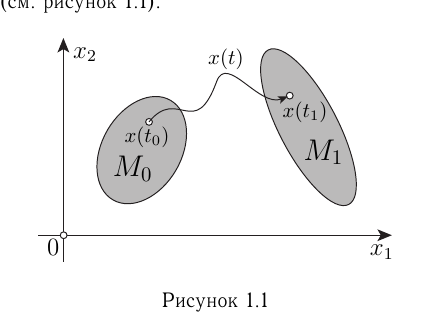
\includegraphics[width=0.72\textwidth]{images/figure_1_1.png}

Рисунок 1.1
\end{center}

Например, в задаче о переводе спутника с одной орбиты на другую множества
$M_0$ и $M_1$ состоят более, чем из одной точки.

Типична ситуация, когда перевод объекта из $M_0$ в $M_1$ может быть выполнен
неединственным способом, при помощи различных допустимых управлений. В этом
случае появляется возможность для оптимизации управляемого процесса, т.е.
можно решать задачу о переводе объекта из $M_0$ в $M_1$ ``наилучшим
способом''. Обсудим сейчас вопрос о том, какой смысл следует приписать
последнему выражению.

\subsubsection{Критерий качества управления}

Рассмотрим пару
\begin{equation}
\bigl(x(t),u(t)\bigr), \qquad t_0 \le t \le t_1,
\end{equation}
где $u(t)$ --- допустимое управление, $x(t)$ --- отвечающая этому управлению
траектория с начальным условием $x(t_0) = x_0 \in M_0$, т.е. $x(t)$ --- решение
задачи Коши (4), причём выполняется условие $x(t_1) \in M_1$.

Рассмотрим также функционал
\begin{equation}
J = \int_{t_0}^{t_1} f^0(t,x(t),u(t))\,dt,
\end{equation}
где $f^0(t,x,u)$ --- известная функция своих аргументов. Таким образом, каждой
паре (7) ставится в соответствие число $J$, определяемое по формуле (8).
Функционал (8) называется критерием качества управления. Он может иметь
физический смысл (в зависимости от функции $f^0$):
\begin{itemize}
\item[а)] расхода топлива,
\item[б)] энергетических затрат,
\item[в)] финансовых затрат или прибыли,
\item[г)] времени перехода из $M_0$ в $M_1$,
\item[д)] и т.д.
\end{itemize}

Конкретный выбор функционала $J$ в приложениях производится инженером,
исходя из требований, предъявляемых к рассматриваемому управляемому процессу.
В случае $f^0 = 1$ получаем
\begin{equation}
J = t_1 - t_0.
\end{equation}

\noindent
(функционал имеет физический смысл времени перехода объекта из $M_0$ в $M_1$).

Нашей целью является минимизация функционала (8), характеризующего качество
процесса управления.

Мы описали выше основные элементы\footnote{В постановку задачи оптимального
управления могут вводиться дополнительные ограничения.}, типичные для
математической задачи оптимального управления, и переходим сейчас к её
постановке.

\subsubsection{Постановка задачи оптимального управления}

Требуется: перевести объект из множества начальных состояний $M_0$, см. (5),
на множество конечных состояний $M_1$, см. (6), за счёт выбора допустимого
управления $u = u(t)$ из класса допустимых управлений $\UU$, так, чтобы
функционал $J$, см. (8), принимал минимальное значение, или в компактной
форме
\[
J \to \min_{u(\cdot)\in\UU}.
\]

Управление $u(t)$, решающее поставленную задачу, называется оптимальным
управлением (в смысле функционала $J$). Траектория $x(t)$, отвечающая
оптимальному управлению $u(t)$, называется оптимальной траекторией. В случае
(9) задача оптимального управления называется задачей быстродействия.

Таким образом, постановка задачи оптимального управления в краткой форме
имеет следующий вид:
\begin{equation}
\left\{
\begin{array}{l}
\dot x(t) = f(t,x,u),\\
u(t) \in \UU,\\
x(t_0) \in M_0,\\
x(t_1) \in M_1,\\
J \to \min\limits_{u(\cdot)\in\UU}.
\end{array}
\right.
\end{equation}

Задача (10) требует задания следующего набора исходных данных:
\begin{equation}
\{f^0, f; \UU = \UU_U; M_0, M_1, t_0\}.
\end{equation}

Напомним ещё раз, что момент времени $t_1$ окончания процесса управления
\begin{itemize}
\item[а)] может быть заранее заданным и в этом случае число $t_1$ следует отнести к набору элементов (11);
\item[б)] может быть незаданным (так обстоит дело, например, в задаче быстродействия, где $t_1$ заранее неизвестен), и в этом случае нахождение $t_1$ следует отнести к задаче нахождения оптимального управления $u(t)$, $t_0 \le t \le t_1$.
\end{itemize}

Заметим, что задача максимизации $I \to \max\limits_{u(\cdot)\in\UU}$ может
быть сведена к задаче минимизации функционала $J = -I$.

\subsubsection{Основные математические вопросы теории оптимального управления}

Перечислим основные вопросы теории оптимального управления.
\begin{enumerate}
\item Управляемость (возможность перевода объекта из $M_0$ в $M_1$ при помощи некоторого допустимого управления; без управляемости решения задачи (10) не существует). Исследование управляемости не связано с критерием качества управления.
\item Существование оптимального управления (пусть объект обладает свойством управляемости; существует ли оптимальное управление в выбранном классе допустимых управлений $\UU$?).
\item Необходимые условия оптимальности (теоремы о необходимых условиях оптимальности в форме принципа максимума Понтрягина [1]). Роль необходимых условий невозможно переоценить; необходимые условия позволяют, вообще говоря, выделить отдельные траектории, которые могут быть оптимальными, отбраковать заведомо неоптимальные решения. Роль необходимых условий оптимальности можно сравнить с ролью условия $f'(x)=0$ в задаче на минимум функции $f(x)$ и с ролью уравнений Эйлера--Лагранжа в классическом вариационном исчислении.
\item Достаточные условия оптимальности.
\item Единственность оптимального управления.
\item Численные методы построения оптимальных решений.
\end{enumerate}

В настоящем курсе излагается линейная теория быстродействия.

\subsubsection{Линейная задача быстродействия}

Линейная задача быстродействия является частным случаем задачи оптимального
управления (10) при условии (9) и в предположении линейности функции $f$:
\begin{align}
\dot x &= Ax + u, \tag{12}\\
x(t_0) &\in M_0,\quad x(t_1) \in M_1, \tag{13}\\
J = t_1 - t_0 &\to \min_{u(\cdot)\in\UU_U}. \tag{14}
\end{align}

Здесь
\[
x =
\begin{pmatrix}
x_1\\
\vdots\\
x_n
\end{pmatrix}
\]
--- вектор фазовых координат; $x \in E^n$,
\[
A = (a_{ij})
\]
--- матрица системы (считаем её независящей от времени $t$),
\[
u =
\begin{pmatrix}
u_1\\
\vdots\\
u_n
\end{pmatrix}
\]
--- вектор управления; $u \in E^n$.

Класс допустимых управлений
\[
\UU = \UU_U =
\left\{
u(t)\
\middle|\
\begin{array}{l}
1)\ \text{принимает значения из компакта } U,\\
2)\ \text{задан характер зависимости } u \text{ от } t
\end{array}
\right\}.
\]

Компакт $U$ называется областью управления.

$M_0$ --- множество начальных состояний объекта,

$M_1$ --- множество конечных состояний объекта,

$J = t_1 - t_0$ --- критерий качества управления (время перехода из $M_0$ в $M_1$).

Линейная задача быстродействия (12)--(14) задаётся набором исходных данных
\begin{equation}
\{A, M_0, M_1, \UU = \UU_U, t_0\}
\end{equation}
и состоит в нахождении допустимого управления $u = u(t)$, переводящего объект
из $M_0$ в $M_1$ по траекториям уравнения (12) за минимальное время.
Управление $u(t)$, решающее эту задачу, называется оптимальным по
быстродействию, а соответствующая этому управлению траектория $x(t)$
называется оптимальной по быстродействию траекторией.

\subsubsection{Два простейших примера}

\textbf{Пример 1.1.} Управляемое движение материальной точки по прямой под
действием ограниченной внешней силы (задача о тележке).

Рассмотрим материальную точку массы $m$, которая движется по прямой
(ось $y$) без трения под действием ограниченной внешней силы,
направленной вдоль оси $y$.

\begin{center}
\begin{tikzpicture}[scale=0.95]
\draw[->] (-2.2,0) -- (2.9,0) node[below] {$y$};
\fill (-1.5,0) circle (1.6pt) node[below=5pt] {$0$};
\draw[fill=white] (1.1,0) circle (0.22) node[above=6pt] {$m$};
\draw[->,line width=0.5pt] (1.45,0.35) -- (2.35,0.35) node[right] {$f(t)$};
\end{tikzpicture}

Рисунок 1.2
\end{center}

Геометрическое положение материальной точки описывается координатой
$y = y(t)$. На основании второго закона Ньютона запишем
дифференциальное уравнение движения точки
\[
m\ddot y = f(t),
\]
т.е.
\begin{equation}
\ddot y = v(t), \tag{16}
\end{equation}
где $v(t) = f(t)/m$ --- управление. Считаем заданными начальные условия
$y(0) = a$ (начальное положение точки), $\dot y(0) = b$ (начальная скорость
точки). Дальнейшее движение точки зависит от выбора управления $v(t)$,
которое при $m = 1$ совпадает с $f(t)$. Пусть управление $v(t)$ подчинено
ограничению
\[
|v(t)| \le 1.
\]

Рассмотрим задачу о переводе точки из начального положения $a$ при
начальной скорости $b$ в положение $y = 0$ с нулевой скоростью.
Этот перевод осуществляется за счёт выбора управления $v(t)$. Требуется
выполнить этот перевод за кратчайшее время.

Полагая $y = x_1$, $\dot y = x_2$, $v = u_2$, перейдём от
дифференциального уравнения (16) второго порядка к следующей системе
дифференциальных уравнений:
\[
\dot x_1 = x_2,\qquad \dot x_2 = u_2.
\]
В данном примере размерность фазового пространства равна $2$, фазовым
пространством служит фазовая плоскость $(x_1,x_2)$. Множество начальных
состояний
\[
M_0 = \left\{
\begin{pmatrix}
a\\
b
\end{pmatrix}
\right\}
\]
состоит из одной точки,
\[
M_1 = \left\{
\begin{pmatrix}
0\\
0
\end{pmatrix}
\right\}
\]
--- начало координат,
\[
x =
\begin{pmatrix}
x_1\\
x_2
\end{pmatrix}
\]
--- фазовый вектор,
\[
A =
\begin{pmatrix}
0 & 1\\
0 & 0
\end{pmatrix},
\]
область управления
\[
U = \left\{
u =
\begin{pmatrix}
u_1\\
u_2
\end{pmatrix}
\ \middle|\
u_1 = 0,\ |u_2| \le 1
\right\}.
\]
Таким образом, мы получили линейную задачу быстродействия в стандартной
форме (12)--(14).

\textbf{Пример 1.2.} Управляемое движение математического маятника под
действием ограниченной внешней силы.

Рассмотрим движение тяжёлого шарика массы $m$ под воздействием
упругой силы пружины и внешней силы $f(t)$ (рисунок 1.3). Задача
рассматривается без учёта силы трения.

\begin{center}
\begin{tikzpicture}[scale=0.95]
\draw (-2.45,-0.6) -- (-2.45,0.6);
\foreach \yy in {-0.5,-0.3,...,0.5} {
  \draw (-2.75,\yy-0.15) -- (-2.45,\yy+0.15);
}
\draw (-2.45,0) -- (-2.05,0);
\draw (-2.05,0) -- (-1.8,0.22) -- (-1.55,-0.22) -- (-1.3,0.22) -- (-1.05,-0.22) -- (-0.8,0.22) -- (-0.55,-0.22) -- (-0.3,0.22) -- (-0.05,-0.22) -- (0.2,0);
\draw[fill=white] (0.85,0) circle (0.22) node[above=6pt] {$m$};
\fill (-1.55,0) circle (1.4pt) node[below=5pt] {$0$};
\draw[->] (-1.55,0) -- (1.8,0) node[below] {$y$};
\draw[->,line width=0.5pt] (1.15,0.35) -- (2.05,0.35) node[right] {$f(t)$};
\end{tikzpicture}

Рисунок 1.3
\end{center}

Движение шарика происходит вдоль оси $y$. В состоянии равновесия шарик
имеет координату $y = 0$. Привлекая физические законы --- второй закон
Ньютона и закон Гука (упругая сила пропорциональна отклонению от
положения равновесия и направлена в сторону положения равновесия), ---
запишем дифференциальное уравнение движения
\[
m\ddot y = -ky + f(t),
\]
где положительный коэффициент $k$ характеризует жёсткость пружины.
Полагая $\omega^2 = k/m$, $v(t) = f(t)/m$, приходим к уравнению
\begin{equation}
\ddot y + y = v(t). \tag{17}
\end{equation}
Здесь мы для упрощения считаем $\omega^2 = 1$, $|v(t)| \le 1$. Пусть
заданы начальные условия $y(0) = a$, $\dot y(0) = b$. Рассмотрим задачу
о скорейшем успокоении маятника под действием ограниченной внешней силы
$v(t)$.

Полагая $y = x_1$, $\dot y = x_2$, $v = u_2$, от уравнения (17) переходим
к системе
\[
\dot x_1 = x_2,\qquad \dot x_2 = -x_1 + u_2.
\]
Как и в предыдущем примере, здесь $n = 2$,
\[
M_0 = \left\{
\begin{pmatrix}
a\\
b
\end{pmatrix}
\right\},\qquad
M_1 = \left\{
\begin{pmatrix}
0\\
0
\end{pmatrix}
\right\},
\]
\[
x =
\begin{pmatrix}
x_1\\
x_2
\end{pmatrix},\qquad
U = \left\{
u =
\begin{pmatrix}
u_1\\
u_2
\end{pmatrix}
\ \middle|\
u_1 = 0,\ |u_2| \le 1
\right\},
\]
но теперь матрица системы имеет вид
\[
A =
\begin{pmatrix}
0 & 1\\
-1 & 0
\end{pmatrix}.
\]
Мы опять пришли к постановке линейной задачи быстродействия в стандартной
форме. Решение этих примеров описывается в разделах 3.13, 3.16.

\subsection{Некоторые сведения из теории обыкновенных дифференциальных уравнений}

При изучении линейной теории оптимального управления важную роль играет
формула Коши для решения линейной системы. В разделе 1.2 приводится
обоснование формулы Коши для линейных систем с постоянными коэффициентами,
изучается экспоненциал матрицы, рассмотрены примеры.

\subsubsection{Формула Коши для решения начальной задачи в случае линейной системы обыкновенных дифференциальных уравнений}

\textit{Скалярный случай} $(n = 1)$. Рассмотрим задачу Коши
\begin{equation}
\dot x = ax + u(t),\qquad x(t_0) = x_0. \tag{1}
\end{equation}
Здесь $x = x(t)$ --- неизвестная скалярная функция аргумента $t$, $u(t)$ ---
известная непрерывная функция, $a$ --- заданное число, $x_0$ --- заданное
начальное условие, $t$ --- независимая переменная (время), $t_0$ ---
начальный момент времени.

Решение задачи Коши (1) определяется следующей формулой:
\begin{equation}
x(t) = e^{(t-t_0)a}
\left(
x_0 + \int_{t_0}^{t} e^{-(s-t_0)a} u(s)\,ds
\right). \tag{2}
\end{equation}

В этом можно убедиться непосредственной проверкой. Действительно, функция
(2) удовлетворяет начальному условию $x(t_0) = x_0$ и является решением
дифференциального уравнения, так как
\[
\begin{aligned}
\dot x(t) &=
a e^{(t-t_0)a}
\left(
x_0 + \int_{t_0}^{t} e^{-(s-t_0)a} u(s)\,ds
\right) \\
&\qquad + e^{-(t-t_0)a} e^{(t-t_0)a} u(t)
= ax(t) + u(t).
\end{aligned}
\]
Формула (2) называется формулой Коши.

\textbf{Замечание 2.1.} Если $u(t)$ --- кусочно-непрерывная функция со
скачками в точках $\tau_1,\ldots,\tau_s$, то формулой (2) определяется
непрерывная кусочно-дифференцируемая функция $x(t)$, которая удовлетворяет
дифференциальному уравнению $\dot x(t) = ax(t) + u(t)$ для всех
$t \ne \tau_1,\ldots,\tau_s$; производная $\dot x(t)$ в точках
$\tau_1,\ldots,\tau_s$ имеет конечные скачки (см. рисунок 2.1).

\begin{center}
\begin{tikzpicture}[x=1cm,y=1cm]
\begin{scope}
\draw[->] (0,0) -- (6.6,0) node[right] {$t$};
\draw[->] (0,-0.1) -- (0,2.2);
\draw (0,-0.05) node[below] {$t_0$};
\draw (1.4,0.08) -- (1.4,-0.08) node[below] {$\tau_1$};
\draw (3.2,0.08) -- (3.2,-0.08) node[below] {$\tau_2$};
\draw (5.2,0.08) -- (5.2,-0.08) node[below] {$\tau_s$};
\draw[line width=0.5pt] (0.2,0.5) -- (1.4,0.5);
\draw[line width=0.5pt] (1.4,1.1) -- (3.2,1.1);
\draw[line width=0.5pt] (3.2,1.55) -- (5.2,1.55);
\draw[line width=0.5pt] (5.2,1.2) -- (6.1,1.2);
\draw[line width=0.5pt] (1.4,0.5) -- (1.4,1.1);
\draw[line width=0.5pt] (3.2,1.1) -- (3.2,1.55);
\draw[line width=0.5pt] (5.2,1.55) -- (5.2,1.2);
\node at (0.9,1.95) {$u = u(t)$};
\end{scope}
\begin{scope}[yshift=-3.2cm]
\draw[->] (0,0) -- (6.6,0) node[right] {$t$};
\draw[->] (0,-0.1) -- (0,2.2);
\draw (0,-0.05) node[below] {$t_0$};
\draw (1.4,0.08) -- (1.4,-0.08) node[below] {$\tau_1$};
\draw (3.2,0.08) -- (3.2,-0.08) node[below] {$\tau_2$};
\draw (5.2,0.08) -- (5.2,-0.08) node[below] {$\tau_s$};
\draw[line width=0.5pt]
  (0.2,0.3) .. controls (0.9,0.55) and (1.1,0.7) .. (1.4,0.82)
  .. controls (1.9,0.98) and (2.5,1.15) .. (3.2,1.28)
  .. controls (3.8,1.4) and (4.5,1.56) .. (5.2,1.66)
  .. controls (5.6,1.72) and (5.9,1.78) .. (6.1,1.84);
\node at (1.0,1.95) {$x = x(t)$};
\end{scope}
\end{tikzpicture}

Рисунок 2.1
\end{center}

\textit{Общий случай} $(n > 1)$. Рассмотрим задачу Коши
\begin{equation}
\dot x = Ax + u(t),\qquad x(t_0) = x_0. \tag{3}
\end{equation}
Здесь
\[
x =
\begin{pmatrix}
x_1\\
\vdots\\
x_n
\end{pmatrix},\qquad
A =
\begin{pmatrix}
a_{11} & \cdots & a_{1n}\\
\vdots & \ddots & \vdots\\
a_{n1} & \cdots & a_{nn}
\end{pmatrix},
\]
\[
u(t) =
\begin{pmatrix}
u_1(t)\\
\vdots\\
u_n(t)
\end{pmatrix},\qquad
x_0 =
\begin{pmatrix}
x_{01}\\
\vdots\\
x_{0n}
\end{pmatrix};
\]
$x = x(t)$ --- неизвестная векторная функция, $u(t)$ --- заданная непрерывная
векторная функция, $A$ --- постоянная квадратная матрица, $x_0$ --- вектор
начальных условий. Решение
\[
x(t) =
\begin{pmatrix}
x_1(t)\\
\vdots\\
x_n(t)
\end{pmatrix}
\]
задачи Коши (3) определяется формулой
\begin{equation}
x(t) = e^{(t-t_0)A}
\left(
x_0 + \int_{t_0}^{t} e^{-(s-t_0)A} u(s)\,ds
\right), \tag{4}
\end{equation}
или
\begin{equation}
x(t) = e^{(t-t_0)A} x_0 + \int_{t_0}^{t} e^{(t-s)A} u(s)\,ds. \tag{5}
\end{equation}
Формулы (4), (5) называются формулами Коши. В однородном случае
($u(t) = 0$) решение задачи Коши $\dot x = Ax$, $x(t_0) = x_0$,
определяется формулой
\begin{equation}
x(t) = e^{(t-t_0)A} x_0. \tag{6}
\end{equation}

В формулах (4)--(6) участвует матричная функция $e^{(t-t_0)A}$, называемая
экспоненциалом матрицы $A$. В разделе 1.2.2 вводится понятие
экспоненциала, изучаются его основные свойства. После этого нетрудно
обосновать формулу Коши.

\subsubsection{Экспоненциал постоянной квадратной матрицы. Его основные свойства. Обоснование формулы Коши}

Рассмотрим квадратную матрицу $n$-го порядка
\[
D =
\begin{pmatrix}
d_{11} & \cdots & d_{1n}\\
\vdots & \ddots & \vdots\\
d_{n1} & \cdots & d_{nn}
\end{pmatrix}
= \bigl((D)_{ij}\bigr)_{i,j=1}^{n},\qquad
(D)_{ij} = d_{ij},\quad i,j = 1,\ldots,n.
\]

Напомним известную из математического анализа формулу
\[
e^t = 1 + \frac{t}{1!} + \frac{t^2}{2!} + \cdots + \frac{t^k}{k!} + \cdots
= \sum_{k=0}^{\infty} \frac{t^k}{k!}.
\]
Этот степенной ряд сходится при всех $t$.

Определим теперь экспоненциал $e^D$ матрицы $D$, положив
\begin{equation}
e^D =
E + \frac{1}{1!} D + \frac{1}{2!} D^2 + \cdots + \frac{1}{k!} D^k + \cdots
= \sum_{k=0}^{\infty} \frac{1}{k!} D^k. \tag{7}
\end{equation}
Здесь $0! = 1$; $D^0 = E$ --- единичная матрица $n$-го порядка.
Таким образом, экспоненциал определён как сумма матричного ряда (7),
члены которого являются квадратными матрицами порядка $n$.
Экспоненциал $e^D$ --- квадратная матрица порядка $n$. Сходимость
матричного ряда (7) понимается в смысле поэлементной сходимости, т.е.
\begin{equation}
(e^D)_{ij} = (E)_{ij} + \frac{1}{1!}(D)_{ij} + \frac{1}{2!}(D^2)_{ij}
+ \cdots + \frac{1}{k!}(D^k)_{ij} + \cdots . \tag{8}
\end{equation}

В случае $D = tA$, где $t$ --- скалярный множитель (в приложениях
$t$ --- время), $A$ --- $(n \times n)$-матрица, получаем
\begin{equation}
e^{tA} = E + \frac{t}{1!} A + \frac{t^2}{2!} A^2 + \cdots
+ \frac{t^k}{k!} A^k + \cdots . \tag{9}
\end{equation}

\textbf{Теорема 2.1} (об основных свойствах экспоненциала).
\begin{enumerate}
\item Для любой $(n \times n)$-матрицы $D$ существует экспоненциал $e^D$ (сходится матричный ряд (7), т.е. сходятся $n^2$ числовых рядов (8)).
\item Если $A$, $B$ --- две перестановочные $(AB = BA)$ $(n \times n)$-матрицы, то
\[
e^A \cdot e^B = e^{A+B}.
\]
\item Матрица $e^D$ невырождена, причём её обратная матрица определяется равенством
\[
\bigl(e^D\bigr)^{-1} = e^{-D}.
\]
\item Пусть $D = tA$; матричная функция $e^{tA}$ непрерывно дифференцируема, причём
\[
\frac{d}{dt} e^{tA} = Ae^{tA} = e^{tA}A.
\]
\end{enumerate}

\textbf{Доказательство.}

\textit{1)} Докажем сходимость числовых рядов (8) для любой матрицы $D$.
Для этого оценим общий член рядов (8). Пусть
\[
|(D)_{ij}| \le d,\qquad i,j = 1,\ldots,n.
\]
Тогда
\[
\bigl(D^2\bigr)_{ij} =
\sum_{\alpha=1}^{n} (D)_{i\alpha}(D)_{\alpha j} \le nd^2,
\]
\[
\bigl(D^3\bigr)_{ij} \le n^2 d^3,
\]
\[
\bigl(D^k\bigr)_{ij} \le n^{k-1} d^k,
\]
и, следовательно, получаем оценку общего члена ряда (8):
\begin{equation}
\frac{1}{k!}(D^k)_{ij} \le \frac{1}{n}\,\frac{(nd)^k}{k!}. \tag{10}
\end{equation}

Теорема сравнения для числовых рядов, сходимость ряда
\[
\sum_{k=1}^{\infty} \frac{1}{n}\,\frac{(nd)^k}{k!}
= \frac{e^{nd}-1}{n}
\]
и неравенство (10) позволяют сделать заключение о сходимости всех
$n^2$ рядов (8), причём эти ряды сходятся абсолютно. Итак, экспоненциал
$e^D$ определён для любой матрицы $D$.

\textit{2)} Пусть $AB = BA$. Тогда
\[
(A + B)^2 = (A + B)(A + B) = A^2 + AB + BA + B^2 = A^2 + 2AB + B^2,
\]
\[
(A + B)^3 = A^3 + 3A^2B + 3AB^2 + B^3,
\]
\[
(A + B)^m = A^m + mA^{m-1}B + \cdots + mAB^{m-1} + B^m
= \sum_{k=0}^{m} \frac{m!}{k!(m-k)!} A^k B^{m-k}
\]
\[
= \sum_{\substack{k+l=m\\k,l\ge 0}} \frac{m!}{k!\,l!} A^k B^l, \tag{11}
\]
т.е. для перестановочных матриц $A$, $B$ имеет место формула бинома
Ньютона, $\dfrac{m!}{k!(m-k)!}$ --- биномиальные коэффициенты. Привлекая
(7), (11), получаем:
\[
\begin{aligned}
e^A \cdot e^B
&=
\left(\sum_{k=0}^{\infty} \frac{1}{k!} A^k \right)
\left(\sum_{l=0}^{\infty} \frac{1}{l!} B^l \right) \\
&=
\sum_{k=0}^{\infty}\sum_{l=0}^{\infty} \frac{1}{k!\,l!} A^k B^l
= \sum_{m=0}^{\infty} \frac{1}{m!}
\left(
\sum_{\substack{k+l=m\\k,l\ge 0}} \frac{m!}{k!\,l!} A^k B^l
\right) \\
&=
\sum_{m=0}^{\infty} \frac{1}{m!} (A+B)^m
= e^{A+B}.
\end{aligned}
\]

\textbf{Задача 2.1.} Привести примеры матриц $A$, $B$, для которых
\[
e^A \cdot e^B \ne e^{A\cdot B}.
\]

\textit{3)} Невырожденность экспоненциала и формула для его обращения
вытекают из части 2) рассматриваемой теоремы. Действительно, в силу
перестановочности матриц $D$ и $(-D)$ получаем:
\[
e^D \cdot e^{-D} = e^{D-D} = e^0 = E,
\]
откуда
\[
\bigl(e^D\bigr)^{-1} = e^{-D}.
\]

\textit{4)} Докажем, что матричная функция $e^{tA}$ непрерывно
дифференцируема по аргументу $t$, т.е. каждый её элемент
$(e^{tA})_{ij}$ --- непрерывно дифференцируемая функция аргумента $t$.
Так как
\begin{equation}
\bigl(e^{tA}\bigr)_{ij}
= \sum_{k=0}^{\infty} \frac{t^k}{k!} (A^k)_{ij} \tag{12}
\end{equation}
--- сумма степенного ряда относительно аргумента $t$ (радиус сходимости
этого ряда равен $\infty$), и степенные ряды можно дифференцировать
сколько угодно раз, причём при дифференцировании радиус сходимости не
изменяется, то функции (12) аналитические. Следовательно, существует
производная $\dfrac{d}{dt}(e^{tA})$, причём
\[
\begin{aligned}
\frac{d}{dt} e^{tA}
&= \frac{d}{dt}
\left(
E + tA + \frac{t^2}{2!}A^2 + \cdots + \frac{t^k}{k!}A^k + \cdots
\right) \\
&= A + tA^2 + \cdots + \frac{t^{k-1}}{(k-1)!}A^k + \cdots \\
&=
A\left(
E + tA + \cdots + \frac{t^{k-1}}{(k-1)!}A^{k-1} + \cdots
\right)
= Ae^{tA} = e^{tA}A.
\end{aligned}
\]
Таким образом,
\begin{equation}
\frac{d}{dt} e^{tA} = A e^{tA},\qquad \left.e^{tA}\right|_{t=0} = E. \tag{13}
\end{equation}

Это свойство экспоненциала позволяет проверить справедливость формулы
Коши при $n > 1$ (подобно тому, как это было сделано выше при $n = 1$).
Действительно, для векторной функции $x(t)$, определяемой формулой (4),
выполняется начальное условие $x(t_0) = x_0$ и, кроме того,
\[
\begin{aligned}
\dot x(t)
&=
Ae^{(t-t_0)A}
\left(
x_0 + \int_{t_0}^{t} e^{-(s-t_0)A}u(s)\,ds
\right)
+ e^{(t-t_0)A} e^{-(t-t_0)A} u(t) \\
&= Ax(t) + u(t),
\end{aligned}
\]
т.е. функция (4) является решением задачи Коши (3). Итак, доказана

\textbf{Теорема 2.2.} Решение задачи Коши (3) существует и определяется
формулой Коши (4) или (5). Кроме того, решение задачи Коши (3)
единственно.

\textbf{Задача 2.2.} Доказать единственность решения задачи Коши (3).

\textbf{Задача 2.3.} Проверить, что
\[
\bigl(e^{tA}\bigr)^* = e^{t(A^*)},\qquad e^{sA}\cdot e^{tA} = e^{(t+s)A},
\]
где $t, s \in E^1$, $*$ --- знак транспонирования.

\textbf{Замечание 2.2.} Если непрерывная функция $u(t)$ определена на
интервале $(a,b)$, содержащем точку $t_0$, то решение задачи (3)
определено на всём интервале $(a,b)$ и описывается на этом интервале
формулой Коши (4). Таким образом, формула Коши (4) применима как при
$t > t_0$, так и при $t < t_0$.

\textbf{Пример.} Найти решение задачи Коши
\[
\dot x = x + 1,\qquad x(0) = 1.
\]
Здесь $n = 1$, $a = 1$, $t_0 = 0$, $x_0 = 1$, $u(\cdot) \equiv 1$.
Применение формулы (2) даёт:
\[
\begin{aligned}
x(t)
&=
e^t \left( 1 + \int_{0}^{t} e^{-s}\cdot 1\,ds \right) \\
&=
e^t \left( 1 + \left.-e^{-s}\right|_{0}^{t} \right)
= e^t(1-e^{-t}+1)
= 2e^t - 1.
\end{aligned}
\]

Формулу Коши (4), (5) целесообразно запомнить, так как исследование
линейной задачи быстродействия основано в значительной степени на
применении формулы Коши.

\subsubsection{Примеры вычисления экспоненциала для конкретных матриц}

\textbf{Пример 2.1.} Найти экспоненциал $e^{tA}$ матрицы
\[
A =
\begin{pmatrix}
0 & 1\\
0 & 0
\end{pmatrix}.
\]
Прямое вычисление даёт $A^2 = 0$; следовательно, $A^k = 0$ при $k \ge 2$,
и ряд (7) содержит лишь два члена:
\[
e^{tA} = E + tA =
\begin{pmatrix}
1 & 0\\
0 & 1
\end{pmatrix}
+ t
\begin{pmatrix}
0 & 1\\
0 & 0
\end{pmatrix}
=
\begin{pmatrix}
1 & t\\
0 & 1
\end{pmatrix}.
\]
Итак,
\[
e^{tA} =
\begin{pmatrix}
1 & t\\
0 & 1
\end{pmatrix},\qquad
e^{-tA} =
\begin{pmatrix}
1 & -t\\
0 & 1
\end{pmatrix},\qquad
e^{-tA^*} =
\begin{pmatrix}
1 & 0\\
-t & 1
\end{pmatrix}.
\]

\textbf{Пример 2.2.} Найти экспоненциал $e^{tA}$ матрицы
\[
A =
\begin{pmatrix}
0 & 1\\
-1 & 0
\end{pmatrix}.
\]
Находим:
\[
\begin{aligned}
A^2 &= -E,\qquad A^3 = -A,\qquad A^4 = E,\qquad A^5 = A,\\
A^6 &= -E,\qquad A^7 = -A,\qquad A^8 = E,\qquad A^9 = A,\ \ldots
\end{aligned}
\]
Применение формулы (7) даёт:
\begin{equation}
\begin{aligned}
e^{tA}
&=
E + tA + \frac{t^2}{2!}(-E) + \frac{t^3}{3!}(-A)
+ \frac{t^4}{4!}E + \frac{t^5}{5!}A + \frac{t^6}{6!}(-E) + \cdots \\
&=
\left(1-\frac{t^2}{2!}+\frac{t^4}{4!}-\cdots\right)E
+ \left(t-\frac{t^3}{3!}+\frac{t^5}{5!}-\cdots\right)A \\
&= \cos t\,E + \sin t\,A.
\end{aligned} \tag{14}
\end{equation}
Таким образом,
\[
e^{tA}
=
\cos t
\begin{pmatrix}
1 & 0\\
0 & 1
\end{pmatrix}
+ \sin t
\begin{pmatrix}
0 & 1\\
-1 & 0
\end{pmatrix}
=
\begin{pmatrix}
\cos t & \sin t\\
-\sin t & \cos t
\end{pmatrix},
\]
\[
e^{-tA}
=
\begin{pmatrix}
\cos t & -\sin t\\
\sin t & \cos t
\end{pmatrix}
=
\bigl(e^{tA}\bigr)^*.
\]

В примерах 2.1, 2.2 экспоненциал $e^{tA}$ получен вычислением ряда (7).
Рассмотрим теперь другой приём нахождения экспоненциала на основе его
свойства (13).

\textbf{Пример 2.3.} Найти экспоненциал $e^{tA}$ матрицы
\[
A =
\begin{pmatrix}
0 & 1\\
0 & -1
\end{pmatrix}.
\]
\textit{1)} Покажем, что
\begin{equation}
e^{tA} =
\begin{pmatrix}
1 & 1-e^{-t}\\
0 & e^{-t}
\end{pmatrix}. \tag{15}
\end{equation}
Для доказательства формулы (15) достаточно проверить, что матрица,
стоящая в правой части (15), удовлетворяет условиям (13). Эта матрица
при $t = 0$ превращается в единичную матрицу, далее
\[
\frac{d}{dt}
\begin{pmatrix}
1 & 1-e^{-t}\\
0 & e^{-t}
\end{pmatrix}
=
\begin{pmatrix}
0 & e^{-t}\\
0 & -e^{-t}
\end{pmatrix}
=
\begin{pmatrix}
0 & 1\\
0 & -1
\end{pmatrix}
\begin{pmatrix}
1 & 1-e^{-t}\\
0 & e^{-t}
\end{pmatrix},
\]
и формула (15) доказана. Недостатком этого способа является то, что не
указан способ получения самой формулы (15).

\textit{2)} Рассмотрим метод получения (15) на основе свойства (13).
Запишем экспоненциал в форме
\[
e^{tA} =
\begin{pmatrix}
y_1(t) & z_1(t)\\
y_2(t) & z_2(t)
\end{pmatrix}
= \bigl(y(t)\ z(t)\bigr).
\]
Его первый столбец
\[
y(t) =
\begin{pmatrix}
y_1(t)\\
y_2(t)
\end{pmatrix}
\]
находим, решая задачу Коши
\[
\dot y = Ay,\qquad y(0) =
\begin{pmatrix}
1\\
0
\end{pmatrix},
\]
причём вектором начальных условий служит первый столбец единичной
матрицы. Последняя система в координатной форме имеет вид:
\[
\dot y_1 = y_2,\qquad y_1(0) = 1,
\]
\[
\dot y_2 = -y_2,\qquad y_2(0) = 0.
\]
Решая её, получаем:
\[
y_1(t) \equiv 1,\qquad y_2(t) \equiv 0,\qquad
y(t) \equiv
\begin{pmatrix}
1\\
0
\end{pmatrix}.
\]

Для нахождения второго столбца $z(t)$ экспоненциала решаем задачу Коши
\[
\dot z = Az,\qquad z(0) =
\begin{pmatrix}
0\\
1
\end{pmatrix}.
\]
Получаем:
\[
z_1(t) = 1-e^{-t},\qquad z_2(t) = e^{-t},\qquad
z(t) =
\begin{pmatrix}
1-e^{-t}\\
e^{-t}
\end{pmatrix}.
\]
Таким образом, мы пришли к формуле (15).

Обратим внимание на то, что экспоненциал (15) может быть записан в форме
\begin{equation}
e^{tA} = p_0(t)E + p_1(t)A, \tag{16}
\end{equation}
где $p_0(t) = 1$, $p_1(t) = 1 - e^{-t}$. Аналогичное представление было
получено для экспоненциала из примера 2.2, см. (14), где
$p_0(t) = \operatorname{ch} t$, $p_1(t) = \operatorname{sh} t$. Это
наблюдение позволяет применить для нахождения экспоненциала следующий
метод.

\textit{3)} Ищем экспоненциал в форме (16), где функции $p_0(t)$, $p_1(t)$
подлежат определению. Полагая в (16) $t = 0$, получаем начальные условия
\begin{equation}
p_0(0) = 1,\qquad p_1(0) = 0. \tag{17}
\end{equation}
Дифференцируя (16) по $t$ и используя свойство (13), получаем
\begin{equation}
A e^{tA} = \dot p_0(t)E + \dot p_1(t)A. \tag{18}
\end{equation}
Подстановка (16) в (18) даёт
\[
p_0(t)A + p_1(t)A^2 = \dot p_0(t)E + \dot p_1(t)A,
\]
откуда, принимая во внимание равенство $A^2 = -A$, находим
\[
\dot p_0(t)E + \bigl(\dot p_1(t) + p_1(t) - p_0(t)\bigr)A = 0.
\]
Следовательно,
\[
\dot p_0(t) = 0,\qquad \dot p_1(t) + p_1(t) - p_0(t) = 0.
\]
Из условий $\dot p_0(t)=0$, $p_0(0)=1$ следует: $p_0(t)\equiv 1$. Далее
из условий $\dot p_1(t)+p_1(t)-p_0(t)=0$, $p_1(0)=0$, $p_0(t)=1$ следует,
что $p_1(t)=1-e^{-t}$. Таким образом, в примере 2.3
\[
e^{tA} = p_0(t)E + p_1(t)A =
\begin{pmatrix}
1 & 1-e^{-t}\\
0 & e^{-t}
\end{pmatrix}.
\]

Выбор представления экспоненциала (16), на котором основан последний
метод, объясняет приведённая в разделе 1.2.4 теорема.

\textbf{Пример 2.4.} Найти экспоненциал $e^{tA}$ для матрицы
\[
A =
\begin{pmatrix}
0 & 1\\
1 & 0
\end{pmatrix}.
\]
\textit{Решение:}
\[
e^{tA} = \operatorname{ch} t \cdot E + \operatorname{sh} t \cdot A =
\begin{pmatrix}
\operatorname{ch} t & \operatorname{sh} t\\
\operatorname{sh} t & \operatorname{ch} t
\end{pmatrix}.
\]

\textbf{Пример 2.5.} Найти $e^{tA}$, где матрица
\[
A =
\begin{pmatrix}
0 & 1 & 0\\
0 & 0 & 1\\
0 & 0 & 0
\end{pmatrix}.
\]
\textit{Решение:} $A^k = 0$, $k \ge 3$, поэтому
\[
e^{tA} = E + tA + \frac{t^2}{2!}A^2 =
\begin{pmatrix}
1 & t & \dfrac{t^2}{2}\\
0 & 1 & t\\
0 & 0 & 1
\end{pmatrix}.
\]

\textbf{Пример 2.6.} Найти $e^{tA}$ для матрицы
\[
A =
\begin{pmatrix}
0 & 0 & 1\\
0 & 1 & 0\\
1 & 0 & 0
\end{pmatrix}.
\]
\textit{Решение:}
\[
A^2 = A^4 = \cdots = A^{2k} = E,\qquad
A^3 = A^5 = \cdots = A^{2k+1} = A,\quad k = 1,2,\ldots,
\]
и по формуле (7) получаем
\[
e^{tA} = \operatorname{ch} t \cdot E + \operatorname{sh} t \cdot A =
\begin{pmatrix}
\operatorname{ch} t & 0 & \operatorname{sh} t\\
0 & e^t & 0\\
\operatorname{sh} t & 0 & \operatorname{ch} t
\end{pmatrix}.
\]

\textbf{Пример 2.7.} Найти $e^{tA}$, где $(n \times n)$-матрица
\[
A =
\begin{pmatrix}
0 & 1 & 0 & \cdots & 0\\
0 & 0 & 1 & \cdots & 0\\
\vdots & \vdots & \vdots & \ddots & \vdots\\
0 & 0 & 0 & \cdots & 1\\
0 & 0 & 0 & \cdots & 0
\end{pmatrix}.
\]
\textit{Решение.} Так как $A^n = 0$, то по формуле (7) получаем:
\[
e^{tA} =
\begin{pmatrix}
1 & t & \dfrac{t^2}{2!} & \cdots & \dfrac{t^{n-1}}{(n-1)!}\\
0 & 1 & t & \cdots & \dfrac{t^{n-2}}{(n-2)!}\\
0 & 0 & 1 & \cdots & \dfrac{t^{n-3}}{(n-3)!}\\
\vdots & \vdots & \vdots & \ddots & \vdots\\
0 & 0 & 0 & \cdots & 1
\end{pmatrix}.
\]

\textbf{Пример 2.8.} Найти экспоненциал $e^{tA}$, где $(n \times n)$-матрица
\[
A =
\begin{pmatrix}
\lambda & 1 & 0 & \cdots & 0\\
0 & \lambda & 1 & \cdots & 0\\
\vdots & \vdots & \ddots & \ddots & \vdots\\
0 & 0 & \cdots & \lambda & 1\\
0 & 0 & \cdots & 0 & \lambda
\end{pmatrix}
\]
(жорданова клетка).

\textbf{Пример 2.9.} Пусть
\[
J = \operatorname{diag}(J_1, J_2, \ldots, J_s)
\]
--- матрица клеточно-диагональной структуры с блоками
\[
J_m =
\begin{pmatrix}
\lambda_m & 1 & 0 & \cdots & 0\\
0 & \lambda_m & 1 & \cdots & 0\\
\vdots & \vdots & \ddots & \ddots & \vdots\\
0 & 0 & \cdots & \lambda_m & 1\\
0 & 0 & \cdots & 0 & \lambda_m
\end{pmatrix},
\qquad m = 1,\ldots,s,
\]
размерности $(k_m \times k_m)$ (жорданова клетка); $k_1 + \cdots + k_s = n$.
Показать, что $(n \times n)$-матрица $J$ имеет экспоненциал
клеточно-диагональной структуры
\[
e^{tJ} =
\begin{pmatrix}
e^{tJ_1} & 0 & \cdots & 0\\
0 & e^{tJ_2} & \cdots & 0\\
\vdots & \vdots & \ddots & \vdots\\
0 & 0 & \cdots & e^{tJ_s}
\end{pmatrix}.
\]

\textbf{Пример 2.10.} Найти $e^{tA}$, если $A = T^{-1}JT$, где $T$ ---
невырожденная $(n \times n)$-матрица, $J$ --- матрица из примера 2.9.
Показать, что
\[
e^{tA} = T^{-1} e^{tJ} T.
\]

Предлагается решить примеры 2.8--2.10 самостоятельно.

\subsubsection{Теорема о представлении экспоненциала в виде конечной суммы}

\textbf{Теорема 2.3.} Пусть $A$ --- квадратная матрица $n$-го порядка,
$t$ --- скалярная переменная. Тогда
\begin{equation}
e^{tA} = \sum_{j=0}^{n-1} p_j(t) A^j, \tag{19}
\end{equation}
где $p_j(t)$ --- скалярные непрерывные (и даже аналитические) функции
аргумента $t$.

\textbf{Доказательство теоремы 2.3} основано на представлении
экспоненциала $e^{tA}$ в форме ряда (7) и теореме Гамильтона--Кэли,
состоящей в том, что матрица аннулирует свой характеристический
многочлен.

Запишем формулу (7) в виде
\begin{equation}
\begin{aligned}
e^{tA} = E + tA + \frac{t^2}{2!}A^2 + \cdots
+ \frac{t^{n-1}}{(n-1)!}A^{n-1}
+ \frac{t^n}{n!}A^n
+ \frac{t^{n+1}}{(n+1)!}A^{n+1}
+ \cdots
\end{aligned}
\tag{20}
\end{equation}

Пусть
\begin{equation}
\begin{aligned}
H_A(\lambda)
&\equiv \det(A-\lambda E) \\
&=
\det
\begin{pmatrix}
a_{11}-\lambda & a_{12} & \cdots & a_{1n}\\
a_{21} & a_{22}-\lambda & \cdots & a_{2n}\\
\vdots & \vdots & \ddots & \vdots\\
a_{n1} & a_{n2} & \cdots & a_{nn}-\lambda
\end{pmatrix} \\
&=
(-1)^n\bigl(\lambda^n - h_{n-1}\lambda^{n-1} - \cdots - h_1\lambda - h_0\bigr)
\end{aligned}
\tag{21}
\end{equation}
--- характеристический многочлен матрицы $A$. Утверждение теоремы
Гамильтона--Кэли можно записать в форме
\begin{equation}
\left. H_A(\lambda)\right|_{\lambda=A} = O, \tag{22}
\end{equation}
где
\[
O =
\begin{pmatrix}
0 & \cdots & 0\\
\vdots & \ddots & \vdots\\
0 & \cdots & 0
\end{pmatrix}
\]
--- нулевая матрица размерности $(n \times n)$.

Из (21), (22) следует, что
\begin{equation}
A^n = q_0^{(n)}E + q_1^{(n)}A + \cdots + q_{n-1}^{(n)}A^{n-1}, \tag{23}
\end{equation}
где $q_j^{(n)} = h_j$, $j = 0,1,\ldots,n-1$, --- коэффициенты
характеристического многочлена (21). Формула (23) показывает, что
$n$-я степень $A^n$ матрицы $A$ линейно выражается через меньшие степени
$A^0 = E$, $A^1$, $A^2$, $\ldots$, $A^{n-1}$ матрицы $A$, причём
коэффициенты $q_j^{(n)}$ в (23) определяются матрицей $A$.

Покажем, что любая степень $A^k$, $k > n$, матрицы $A$ также линейно
выражается через $A^0$, $A^1$, $A^2$, $\ldots$, $A^{n-1}$ с некоторыми
коэффициентами, зависящими от номера $k$ (и от матрицы $A$).
Действительно, умножив равенство (23) на матрицу $A$, получаем:
\begin{equation}
\begin{aligned}
A^{n+1}
&=
q_0^{(n)}A + q_1^{(n)}A^2 + \cdots + q_{n-2}^{(n)}A^{n-1}
+ q_{n-1}^{(n)}A^n \\
&=
q_0^{(n)}A + q_1^{(n)}A^2 + \cdots + q_{n-2}^{(n)}A^{n-1} \\
&\qquad
+ q_{n-1}^{(n)}
\bigl(
q_0^{(n)}E + q_1^{(n)}A + \cdots + q_{n-1}^{(n)}A^{n-1}
\bigr) \\
&=
q_0^{(n+1)}E + q_1^{(n+1)}A + \cdots + q_{n-1}^{(n+1)}A^{n-1}.
\end{aligned}
\tag{24}
\end{equation}

% Auto-generated OCR continuation from raw_text/page_029.txt to page_265.txt
% The first pages remain manually cleaned; the remainder is promoted into editable LaTeX text.

% page 029
где
\[
q_0^{(n+1)} = q_{n-1}^{(n)}q_0^{(n)},\qquad
q_1^{(n+1)} = q_0^{(n)} + q_{n-1}^{(n)}q_1^{(n)},
\]
\[
q_2^{(n+1)} = q_1^{(n)} + q_{n-1}^{(n)}q_2^{(n)},\qquad \ldots,\qquad
q_{n-1}^{(n+1)} = q_{n-2}^{(n)} + q_{n-1}^{(n)}q_{n-1}^{(n)}.
\]

Аналогично получаем:
\begin{equation}
A^{n+2} = q_0^{(n+2)}E + q_1^{(n+2)}A + \cdots + q_{n-1}^{(n+2)}A^{n-1}, \tag{25}
\end{equation}
\begin{equation}
A^{n+s} = q_0^{(n+s)}E + q_1^{(n+s)}A + \cdots + q_{n-1}^{(n+s)}A^{n-1}. \tag{26}
\end{equation}

И так далее. Подстановка соотношений (24)--(26) в ряд (20) приводит
(после перегруппировки членов) к представлению (19) экспоненциала
$e^{tA}$.

\textbf{Упражнение 2.1.} Выписать ряды для коэффициентов
$p_0(t), p_1(t), \ldots, p_{n-1}(t)$ в формуле (19) и доказать
сходимость этих рядов при любом $t$.

\textbf{Замечание 2.3.} В формуле (19) фактически могут отсутствовать
несколько старших степеней матрицы $A$. Например, для матрицы
\[
A =
\begin{pmatrix}
0 & 0 & 1\\
0 & 1 & 0\\
1 & 0 & 0
\end{pmatrix}
\]
из примера 2.6, где $n = 3$, мы получили
$e^{tA} = \operatorname{ch}(t)\cdot E + \operatorname{sh}(t)\cdot A$, т.е.
здесь в представлении экспоненциала
\[
e^{tA} = p_0(t)E + p_1(t)A + p_2(t)A^2
\]
имеем
\[
n - 1 = 2,\qquad p_0(t) = \operatorname{ch}(t),\qquad
p_1(t) = \operatorname{sh}(t),\qquad p_2(t) = 0,
\]
член с $A^2$ фактически отсутствует. В случае $A = E$ имеем
\[
e^{tA} = e^t \cdot E,
\]
т.е. здесь
\[
p_0(t) = e^t,\qquad p_1(t) = \cdots = p_{n-1}(t) = 0.
\]

Теорема 2.3 будет использоваться в разделе 3.15 при доказательстве
леммы о внутренней точке интеграла.

% page 030
\subsubsection{Пример применения формулы Коши для нахождения решения линейных систем}

Задача Коши
\begin{equation}
\ddot y = u_2(t),\qquad y(0) = a_1,\qquad \dot y(0) = a_2 \tag{27}
\end{equation}
где $u_2(t)$ --- заданная функция, $a_1$, $a_2$ --- заданные числа,
может быть решена двумя последовательными интегрированиями:
\[
\dot y(t) = \dot y(0) + \int_0^t \ddot y(s)\,ds = a_2 + \int_0^t u_2(s)\,ds,
\]
\[
\begin{aligned}
y(t)
&= y(0) + \int_0^t \dot y(\tau)\,d\tau
= a_1 + \int_0^t \left(a_2 + \int_0^\tau u_2(s)\,ds\right)d\tau \\
&= a_1 + a_2 t + \int_0^t (t-s)u_2(s)\,ds.
\end{aligned}
\]

Полагая $x_1 = y$, $x_2 = \dot y$, запишем задачу (27) в виде
\[
\dot x_1 = x_2,\qquad x_1(0) = a_1,
\]
\[
\dot x_2 = u_2,\qquad x_2(0) = a_2,
\]
или
\[
\dot x = Ax + u,
\]
где
\[
x =
\begin{pmatrix}
x_1\\
x_2
\end{pmatrix},
\qquad
A =
\begin{pmatrix}
0 & 1\\
0 & 0
\end{pmatrix},
\qquad
x(0) =
\begin{pmatrix}
a_1\\
a_2
\end{pmatrix},
\qquad
u(t) =
\begin{pmatrix}
0\\
u_2(t)
\end{pmatrix}.
\tag{28}
\]

Найдём решение задачи (28), применяя формулу Коши (5). Имеем:
\[
\begin{aligned}
x(t)
&=
\begin{pmatrix}
x_1(t)\\
x_2(t)
\end{pmatrix}
=
\begin{pmatrix}
1 & t\\
0 & 1
\end{pmatrix}
\begin{pmatrix}
a_1\\
a_2
\end{pmatrix}
+ \int_0^t
\begin{pmatrix}
1 & t-s\\
0 & 1
\end{pmatrix}
\begin{pmatrix}
0\\
u_2(s)
\end{pmatrix}
\,ds \\
&=
\begin{pmatrix}
a_1 + a_2 t\\
a_2
\end{pmatrix}
+ \int_0^t
\begin{pmatrix}
(t-s)u_2(s)\\
u_2(s)
\end{pmatrix}
\,ds \\
&=
\begin{pmatrix}
a_1 + a_2 t + \int_0^t (t-s)u_2(s)\,ds\\
a_2 + \int_0^t u_2(s)\,ds
\end{pmatrix},
\end{aligned}
\]
т.е.
\[
x_1(t) = a_1 + a_2 t + \int_0^t (t-s)u_2(s)\,ds = y(t),
\]
\[
x_2(t) = a_2 + \int_0^t u_2(s)\,ds = \dot y(t).
\]

\textbf{Упражнение 2.2.} Найти решение задачи Коши:
\[
1)\ \ddot y + y = u_2(t),\qquad y(0) = a_1,\qquad \dot y(0) = a_2;
\]
\[
2)\ \dddot y = u_3(t),\qquad y(0) = a_1,\qquad \dot y(0) = a_2,\qquad \ddot y(0) = a_3.
\]

\subsubsection{Явная формула для решения задачи Коши в случае одномерного линейного неоднородного дифференциального уравнения с переменными коэффициентами}

Рассмотрим следующую задачу Коши
\begin{equation}
\dot x = a(t)x + b(t),\qquad x(t_0) = x_0, \tag{29}
\end{equation}
где $a(t)$, $b(t)$ --- известные непрерывные функции. Решение $x(t)$
задачи Коши (29) определяется формулой
\begin{equation}
x(t) = e^{A(t)}
\left(
x_0 + \int_{t_0}^t e^{-A(s)}b(s)\,ds
\right), \tag{30}
\end{equation}
где функция $A(t)$ имеет вид
\[
A(t) = \int_{t_0}^t a(s)\,ds.
\]

\textbf{Упражнение 2.3.} Проверить формулу (30).

% page 032
\subsection{Множество достижимости, множество управляемости. Их представление на основе формулы Коши. Предварительные соображения о решении линейной задачи быстродействия}

Рассмотрим линейную задачу быстродействия
\[
\dot x = Ax + u,\qquad x(t_0)\in M_0,\qquad x(t_1)\in M_1,\qquad
t_1 - t_0 \to \min
\]
с классом допустимых управлений $\UU = \UU_U$. При изучении этой задачи
важную роль играют два множества --- множество достижимости и множество
управляемости.

\subsubsection{Множество достижимости $X(t) = X(t_0,t,M_0)$}

Введём множество $X(t_0,\tau,M_0)$, определяемое множеством $M_0$,
начальным моментом времени $t_0$, числом $\tau > t_0$.
Это множество зависит также от матрицы $A$ и от класса допустимых
управлений $\UU = \UU_U$. Рассмотрим задачу Коши
\begin{equation}
\dot x = Ax + u(t),\qquad t_0 \le t \le \tau,\qquad x(t_0) = x_0 \in M_0. \tag{1}
\end{equation}
И выпишем её решение по формуле Коши:
\begin{equation}
x(t) = e^{(t-t_0)A}x_0 + \int_{t_0}^t e^{(t-s)A}u(s)\,ds. \tag{2}
\end{equation}

Поставим вопрос: куда можно перейти к моменту времени $\tau$ по
траекториям дифференциального уравнения (1), исходящим в начальный
момент времени $t_0$ из различных точек $x_0 \in M_0$, если разрешается
использовать всевозможные допустимые управления $u(\cdot)\in\UU$?
Множество концов $x(\tau)$ описанных выше траекторий образует некоторое
множество в $E^n$, которое называется множеством достижимости и
обозначается $X(t_0,\tau,M_0)$ (см. рисунок 3.1). Таким образом,
\begin{equation}
X(t_0,\tau,M_0) =
\left\{
x \in E^n\ \middle|\
\begin{array}{l}
x = x(\tau),\ \text{формула (2) при } t = \tau,\\
x(t_0) \in M_0,\ u(\cdot)\in \UU
\end{array}
\right\}.
\tag{3}
\end{equation}

\begin{center}
Рисунок 3.1
\end{center}

Или, в более подробной записи,
\begin{equation}
X(t_0,\tau,M_0) =
\left\{
x \in E^n\ \middle|\
x = e^{(\tau-t_0)A}x_0 + \int_{t_0}^\tau e^{(\tau-s)A}u(s)\,ds,\
x_0 \in M_0,\ u(\cdot)\in \UU
\right\}.
\tag{4}
\end{equation}
Или
\begin{equation}
X(t_0,\tau,M_0) =
\left\{
e^{(\tau-t_0)A}x_0 + \int_{t_0}^\tau e^{(\tau-s)A}u(s)\,ds
\ \middle|\
x_0 \in M_0,\ u(\cdot)\in \UU
\right\}.
\tag{5}
\end{equation}

Естественно считать, что
\[
X(t_0,t,M_0)\big|_{t=t_0} = M_0.
\]
Для множества достижимости часто удобно использовать краткое
обозначение: $X(t) \equiv X(t_0,t,M_0)$. Множество $X(t)$ с ростом $t$
изменяется. При достаточно малых значениях $t-t_0>0$ множество
$X(t)\cap M_1 = \varnothing$ (см. рисунок 3.2). Если $t_1-t_0$ ---
оптимальное время перехода из $M_0$ в $M_1$, то
\[
X(t)\cap M_1 = \varnothing \quad \text{при } t_0 \le t < t_1,\qquad
X(t_1)\cap M_1 \ne \varnothing.
\]
Подчеркнём, что априори ниоткуда не следует, что множество
достижимости $X(t)$ в процессе изменения с течением времени войдёт
в контакт с множеством $M_1$.

\begin{center}
Рисунок 3.2
\end{center}

\subsubsection{Множество управляемости $Z(t)=Z(t,t_1,M_1)$}

Введём множество $Z(\tau,t_1,M_1)$, определяемое множеством $M_1$,
моментом времени $t_1$, числом $\tau < t_1$ (это множество зависит
также от матрицы $A$ и от класса допустимых управлений $\UU=\UU_U$).
Рассмотрим задачу Коши
\begin{equation}
\dot x = Ax + u(t),\qquad \tau \le t \le t_1,\qquad x(t_1) = x_1 \in M_1.
\tag{6}
\end{equation}
Начальное условие в этой задаче задаётся на правом конце отрезка
$[\tau,t_1]$. Выпишем её решение по формуле Коши:
\begin{equation}
x(t) = e^{(t-t_1)A}x_1 + \int_{t_1}^t e^{(t-s)A}u(s)\,ds
= e^{(t-t_1)A}x_1 + \int_t^{t_1} e^{(t-s)A}[-u(s)]\,ds.
\tag{7}
\end{equation}

Множество $Z(\tau,t_1,M_1)$ (множество управляемости) состоит из всех
таких точек $z \in E^n$, находясь в которых в момент времени $\tau$,
объект в момент времени $t_1$ попадает на множество $M_1$ при помощи
некоторого допустимого управления:
\begin{equation}
Z(\tau,t_1,M_1) =
\left\{
z \in E^n\ \middle|\
\begin{array}{l}
z = x(\tau),\ \text{формула (7) при } t = \tau;\\
x(t_1) \in M_1,\ u(\cdot)\in \UU
\end{array}
\right\}.
\tag{8}
\end{equation}

Или, в более подробной записи,
\begin{equation}
Z(\tau,t_1,M_1) =
\left\{
z \in E^n\ \middle|\
z = e^{(\tau-t_1)A}x_1 + \int_\tau^{t_1} e^{(\tau-s)A}[-u(s)]\,ds,\
x_1 \in M_1,\ u(\cdot)\in \UU
\right\}.
\tag{9}
\end{equation}
или
\begin{equation}
Z(\tau,t_1,M_1) =
\left\{
e^{(\tau-t_1)A}x_1 + \int_\tau^{t_1} e^{(\tau-s)A}[-u(s)]\,ds
\ \middle|\
x_1 \in M_1,\ u(\cdot)\in \UU
\right\}.
\tag{10}
\end{equation}

Естественно считать, что
\[
Z(t,t_1,M_1)\big|_{t=t_1} = M_1.
\]
Для множества управляемости удобно использовать краткое обозначение:
$Z(t)\equiv Z(t,t_1,M_1)$. Свойства множеств $X(t)$, $Z(t)$ рассмотрены
в разделе 3.8. В случае $t_1-t_0=\min$ между множествами $X(t)$ и
$Z(t)$ имеется тесная связь, описанная в разделе 3.11.

\subsubsection{Представление множеств достижимости и управляемости}

на основе формулы Коши

Имеют место следующие представления:
\begin{equation}
X(t_0,t,M_0) = e^{(t-t_0)A}M_0 + \int_{t_0}^t e^{(t-s)A}\UU\,ds,
\tag{11}
\end{equation}
\begin{equation}
Z(t,t_1,M_1) = e^{(t-t_1)A}M_1 + \int_t^{t_1} e^{(t-s)A}[-\UU]\,ds.
\tag{12}
\end{equation}

Обсудим структуру правых частей формул (11), (12). Первые слагаемые
имеют вид произведения матрицы (экспоненциала) на множество, а вторые
слагаемые имеют вид интеграла от класса допустимых управлений $\UU$.
Для обоснования формул (11), (12) ниже вводятся линейные операции над
множествами в пространстве $E^n$, а также операция интегрирования
класса допустимых управлений $\UU$.


% page 036
\subsubsection{Операции над множествами в пространстве $E^n$}

\textbf{Определение 3.1.} Алгебраической суммой двух множеств
$F_1$, $F_2 \subset E^n$ называется множество
\[
F_1 + F_2 = \{x \in E^n : x = f_1 + f_2,\ f_1 \in F_1,\ f_2 \in F_2\},
\]
т.е.
\[
F_1 + F_2 = \{f_1 + f_2 \mid f_1 \in F_1,\ f_2 \in F_2\}.
\]

\textbf{Пример 3.1.} Пусть
\[
F_1 = \{x \in E^2 : |x_1| \le 1,\ x_2 = 0\},\qquad
F_2 = \{x \in E^2 : x_1 = 0,\ |x_2| \le 1\}
\]
--- отрезки. Множество $F = F_1 + F_2$ есть квадрат
\[
\{x \in E^2 : |x_1| \le 1,\ |x_2| \le 1\}
\]
(см. рисунок 3.3).

\begin{center}
Рисунок 3.3
\end{center}

\textbf{Пример 3.2.} Пусть $F_1 = \{a\}$ --- множество, состоящее из
одной точки $a \in E^2$, $F_2 = S_r(0)$ --- круг. Тогда
$F_1 + F_2 = \{a\} + S_r(0) = S_r(a)$ есть круг радиуса $r$ с центром
в точке $a$ (см. рисунок 3.4).


% page 037
\begin{center}
Рисунок 3.4
\end{center}

\textbf{Определение 3.2.} Произведением $(n \times n)$-матрицы $D$ на
множество $F \subset E^n$ называется множество
\[
DF = \{x \in E^n : x = Df,\ f \in F\},
\]
т.е.
\[
DF = \{Df \mid f \in F\}.
\]

\textbf{Пример 3.3.} Пусть
\[
D = \frac{1}{\sqrt2}
\begin{pmatrix}
1 & 1\\
-1 & 1
\end{pmatrix},
\qquad
F = \{x \in E^2 : |x_1| \le 1,\ x_2 = 0\}.
\]
Тогда
\[
DF = \left\{x \in E^2 : x_2 = -x_1,\ |x_1| \le \frac{1}{\sqrt2}\right\}
\]
--- отрезок (см. рисунок 3.5).

\textbf{Определение 3.3} (интеграл от класса допустимых управлений).
Пусть $\UU$ --- класс допустимых управлений, $D(s)$ --- $(n \times n)$-матрица,
непрерывно зависящая от скалярного аргумента $s \in [t_0,t]$; $t_0 < t$.
Полагаем
\[
\int_{t_0}^t D(s)\UU\,ds =
\left\{
x \in E^n\ \middle|\
x = \int_{t_0}^t D(s)u(s)\,ds,\ u(\cdot)\in\UU
\right\},
\]
\[
\int_{t_0}^t D(s)[-\UU]\,ds =
\left\{
x \in E^n\ \middle|\
x = \int_{t_0}^t D(s)[-u(s)]\,ds,\ u(\cdot)\in\UU
\right\}.
\]

\begin{center}
Рисунок 3.5
\end{center}

Из формул (5), (10) и определений 3.1, 3.2, 3.3 следуют
представления (11), (12).


% page 039
\section{Элементы выпуклого анализа в пространстве $E^n$. Три теоремы об интегралах}

\subsection{Основные обозначения и определения. Наименьшая выпуклая оболочка множества и её построение. Лемма об отделимости}

\subsubsection{Основные обозначения и определения}

$E^n$ --- $n$-мерное евклидово пространство,
\[
x =
\begin{pmatrix}
x_1\\
\vdots\\
x_n
\end{pmatrix},
\qquad
y =
\begin{pmatrix}
y_1\\
\vdots\\
y_n
\end{pmatrix},
\qquad \ldots
\]
--- элементы пространства $E^n$,
\[
(x,y) = x_1y_1 + \cdots + x_ny_n
\]
--- скалярное произведение элементов $x$ и $y$,
\[
\|x\| = (x,x)^{1/2}
\]
--- норма элемента $x$,
\[
\|x-y\| = \left(\sum_{i=1}^n (x_i-y_i)^2\right)^{1/2}
\]
--- расстояние между элементами $x$ и $y$,
\[
F
\]
--- множество, лежащее в пространстве $E^n$,
\[
S_r(a) = \{x \in E^n : \|x-a\| \le r\}
\]
--- шар радиуса $r$ с центром в точке $a$ $(r \ge 0,\ a \in E^n)$,
\[
S = \{x \in E^n : \|x\| = 1\}
\]
--- единичная сфера с центром в точке $0$ $(0 \in E^n)$,
\[
\square
\]
--- начало доказательства,
\[
\blacksquare
\]
--- конец доказательства.

\textbf{Определение 4.1.} Множество $F$ называется \textit{открытым},
если для любой точки $x \in F$ существует число $\varepsilon > 0$
такое, что $S_\varepsilon(x) \subset F$
\[
(\forall x \in F\ \exists \varepsilon > 0:\ S_\varepsilon(x) \subset F)
\]
(см. рисунок 4.1).

Множества
\[
F_1 = \{x = (x_1,x_2) \in E^2 : |x_1| < 1,\ |x_2| < 1\},
\]
\[
F_2 = \{x = (x_1,x_2) \in E^2 : x_1^2 + x_2^2 < 1\}
\]
являются открытыми в $E^2$; множества $S_r(a)$, $S$ не являются
открытыми.

\textbf{Определение 4.2.} Точка $a \in E^n$ называется
\textit{предельной точкой множества $F$}, если $\forall \varepsilon > 0$
выполняется условие
\[
S_\varepsilon(a) \cap F \ne \varnothing.
\]


% page 040
Так, для множества
\[
F = \{x \in E^n : \|x\| < 1\}
\]
все его предельные точки образуют множество $\mathring S_1(0)$.

\textbf{Определение 4.3.} Множество $F$ называется \textit{замкнутым},
если оно содержит все свои предельные точки.

Множества $S_r(0)$, $S$ замкнуты.

\textbf{Определение 4.4.} Множество $F$ называется
\textit{ограниченным}, если существует такое число $R > 0$, что имеет
место включение $F \subset S_R(0)$, см. рисунок 4.2.

\begin{center}
Рисунок 4.1
\end{center}

\begin{center}
Рисунок 4.2
\end{center}

\textbf{Определение 4.5.} \textit{Модулем множества $F$} называется
число
\[
|F| = \sup_{f \in F}\|f\| = \inf_{r \ge 0}\{r : F \subset S_r(0)\}.
\]

Для любого ограниченного множества $F$ его модуль $|F| < \infty$.
Модуль множества
\[
F = \{x \in E^2 : |x_1| \le 1,\ |x_2| \le 1\}
\]
равен $\sqrt2$.

\textbf{Определение 4.6.} Множество $F$ называется \textit{компактом},
если оно замкнуто и ограничено.

Примерами компактов являются множества
\[
S_r(0),\quad S,\quad F = \{x \in E^2 : |x_1| \le 1,\ |x_2| \le 1\};
\]
множества
\[
F_1 = S_1(0)\setminus\{0\},\qquad F_2 = S_1(0)\setminus S
\]
не являются компактами (нет замкнутости); множество
\[
F_3 = \{x \in E^2 : x_2 \ge 0\}
\]
(полуплоскость) не является компактом (нет ограниченности).


% page 041
\textbf{Определение 4.7.} $\Omega(E^n)$ --- множество, элементами
которого являются всевозможные непустые компакты пространства $E^n$.

\textbf{Определение 4.8.} Пусть $x$, $y$ --- точки пространства $E^n$.
\textit{Отрезком $[x,y]$ с концами $x$, $y$} называется множество
\[
[x,y] = \{z \in E^n : z = \lambda x + (1-\lambda)y,\ \lambda \in [0,1]\},
\]
или
\[
[x,y] = \bigcup_{\lambda \in [0,1]} \{\lambda x + (1-\lambda)y\}.
\]

\textbf{Определение 4.9.} Множество $F$ называется \textit{выпуклым},
если
\[
x,y \in F \Rightarrow [x,y] \subset F.
\]
Так, множество $S_r(a)$ выпукло, а множество $S$ невыпукло.
На рисунке 4.3 изображено невыпуклое множество.

\begin{center}
Рисунок 4.3
\end{center}

\textbf{Определение 4.10.} $\operatorname{conv}\Omega(E^n)$ --- множество,
состоящее из непустых выпуклых компактов пространства $E^n$.
Ясно, что
\[
\operatorname{conv}\Omega(E^n) \subset \Omega(E^n).
\]

\subsubsection{Наименьшая выпуклая оболочка множества и её построение}

\textbf{Определение 4.11.} Множество $G \subset E^n$ называется
\textit{выпуклой оболочкой множества $F$}, если $G$ выпукло и $G \supset F$.
Выпуклая оболочка множества определяется неединственным образом,
см. рисунок 4.4.

\textbf{Определение 4.12.} Множество $H$ называется \textit{наименьшей
выпуклой оболочкой множества $F$}, если


% page 042
\begin{center}
Рисунок 4.4
\end{center}

1. $H$ --- выпуклая оболочка,

2. для любой выпуклой оболочки $G$ множества $F$ выполняется
включение $G \supset H$.

Обозначение наименьшей выпуклой оболочки множества:
\[
H = \operatorname{conv} F.
\]

Для невыпуклого множества $F$, изображенного на рисунке 4.5 а),
наименьшая выпуклая оболочка $\operatorname{conv} F$ изображена
на рисунке 4.5 б).

\begin{center}
Рисунок 4.5
\end{center}

Если множество $F$ выпукло, то $\operatorname{conv} F = F$.
Для множества $F$, состоящего из трёх точек (рисунок 4.6),
$\operatorname{conv} F$ есть треугольник.

\textbf{Теорема 4.1} (о построении наименьшей выпуклой оболочки).
Для любого множества $F \subset E^n$ существует наименьшая выпуклая
оболочка $\operatorname{conv} F$, которую можно построить следующим
образом. Рассмотрим последовательность множеств


% page 043
\begin{center}
Рисунок 4.6
\end{center}

\[
F_0 = F,\qquad \ldots \ldots \ldots \ldots \ldots \ldots
\]
\[
F_1 = \bigcup_{x,y \in F_0}[x,y],\qquad
F_{m+1} = \bigcup_{x,y \in F_m}[x,y],
\]
\[
F_2 = \bigcup_{x,y \in F_1}[x,y],\qquad
\ldots \ldots \ldots \ldots \ldots \ldots
\]

Положим
\[
H = \bigcup_{m=0}^{\infty} F_m.
\]
Тогда $H = \operatorname{conv} F$.

\[
\square
\]
Для доказательства теоремы следует показать, что

1. $F \subset H$,

2. множество $H$ выпукло,

3. любая выпуклая оболочка $G$ множества $F$ содержит множество $H$:
$G \supset H$

(см. определения 4.11, 4.12).

Из построения множеств $F_m$, $H$ следует свойство монотонности:
\[
F = F_0 \subset F_1 \subset F_2 \subset \cdots \subset F_m \subset \cdots \subset H.
\]

Проверим выпуклость множества $H$:
\[
x,y \in H \Rightarrow [x,y] \subset H.
\]
Возьмём две точки $x$, $y \in H$. Существует такой номер $m_1$, что
$x \in F_{m_1}$; существует такой номер $m_2$, что $y \in F_{m_2}$.
Тогда из свойства монотонности следует, что $x,y \in F_m$, где
$m = \max\{m_1,m_2\}$, и, привлекая определение множества $F_{m+1}$,
получаем, что отрезок $[x,y] \subset F_{m+1} \subset H$.
Доказана выпуклость множества $H$. Итак, $H$ --- выпуклая оболочка
множества $F$.


% page 044
Пусть теперь $G$ --- любая выпуклая оболочка множества $F$. Тогда
\[
F = F_0 \subset G,\qquad \ldots \ldots \ldots
\]
\[
F_1 \subset G,\qquad F_{m+1} \subset G,
\]
\[
F_2 \subset G,\qquad \ldots \ldots \ldots
\]
\[
H = \bigcup_{m=0}^{\infty} F_m \subset G,
\]
т.е. доказано, что $H = \operatorname{conv} F$.
\[
\blacksquare
\]

\textbf{Замечание 4.1} (о стабилизации цепочки множеств $\{F_m\}$ в
конечномерном пространстве $E^n$). Существует такой наименьший номер
$s = s(n,F)$, что
\[
F_s = F_{s+1} = \ldots = H,
\]
причём $0 \le s \le n$. Так, например, для выпуклого множества $F$
имеем $F_0 = F_1 = \ldots = H$, т.е. $s = 0$. Для множества $F$,
состоящего из отрезка и точки, не лежащей на этом отрезке
(рисунок 4.7),

\begin{center}
Рисунок 4.7
\end{center}

имеем:
\[
n = 2,\quad s = 1,\quad F_0 \ne F_1 = F_2 = \ldots = H.
\]
Для множества $F$, рассмотренного выше (рисунок 4.6),
$n = 2,\ s = 2$,
\[
F_0 \subset F_1 \subset F_2 = F_3 = \ldots = H,\qquad
F_0 \ne F_1,\ F_1 \ne F_2.
\]

\textbf{Замечание 4.2} (об эквивалентной формулировке процесса
построения наименьшей выпуклой оболочки множества). Последовательность
множеств $\{F_m\}$, введённая в теореме 4.1, может быть определена
соотношениями
\[
F_0 = F,\qquad
F_{m+1} = \bigcup_{\lambda \in [0,1]} \{\lambda F_m + (1-\lambda)F_m\},
\qquad m = 0,1,\ldots
\]


% page 045
Действительно,
\[
F_{m+1} = \bigcup_{x,y \in F_m}[x,y]
= \bigcup_{x,y \in F_m}\bigcup_{\lambda \in [0,1]}
\{\lambda x + (1-\lambda)y\}
\]
\[
= \bigcup_{\lambda \in [0,1]}\bigcup_{x,y \in F_m}
\{\lambda x + (1-\lambda)y\}
= \bigcup_{\lambda \in [0,1]}
\{\lambda F_m + (1-\lambda)F_m\}.
\]

\textbf{Задача 4.1.} Установить включение
$F \subset \lambda F + (1-\lambda)F$ $\forall \lambda \in [0,1]$.
Включение $F \supset \lambda F + (1-\lambda)F$, $\lambda \in (0,1)$,
может не выполняться. Так при $n = 1$, $F = \{-1,+1\}$,
$\lambda = \frac12$ имеем
\[
\frac12 F + \frac12 F = \{-1,0,+1\},
\]
т.е. множество $F$ не содержит множество
$\frac12 F + \frac12 F$.

\textbf{Задача 4.2.} Показать, что для выпуклого множества $F$ при
любом $\lambda \in [0,1]$ выполняется равенство
\[
F = \lambda F + (1-\lambda)F.
\]

\textbf{Задача 4.3.} Алгебраическая сумма $F_1 + F_2$ выпуклых множеств
$F_1$, $F_2$ является выпуклым множеством.

\textbf{Задача 4.4.} Если $F$ --- выпуклое множество,
$D$ --- $(n \times n)$-матрица, то множество $DF$ выпукло.

\textbf{Задача 4.5.} Доказать утверждение о стабилизации цепочки
множеств $\{F_m\}$ в конечномерном пространстве $E^n$,
см. замечание 4.1.

\textbf{Задача 4.6.} Если $F \in \Omega(E^n)$, то
$\operatorname{conv} F \in \operatorname{conv}\Omega(E^n)$.

\subsubsection{Лемма об отделимости (строгая отделимость) и её геометрическая интерпретация. Опорная гиперплоскость}

\textbf{Лемма 4.1.} Пусть

1. $H \in \operatorname{conv}\Omega(E^n)$
(т.е. множество $H$ --- выпуклый компакт),

2. $x_0 \notin H$ (т.е. точка $x_0$ не принадлежит компакту $H$),

тогда
\begin{equation}
\exists\, \psi \in E^n,\ \psi \ne 0:\quad
(h-x_0,\psi) < 0 \quad \forall h \in H,
\tag{1}
\end{equation}
\begin{equation}
\exists\, \psi_0 \in S:\quad
(h-x_0,\psi_0) < 0 \quad \forall h \in H.
\tag{2}
\end{equation}

Утверждения (1) и (2) равносильны. Лемма об отделимости имеет простой
геометрический смысл (рисунок 4.8):


% page 046
\begin{center}
Рисунок 4.8
\end{center}

через точку $x_0$ можно провести гиперплоскость $\Gamma_\psi$ с
вектором нормали $\psi$ такую, что компакт $H$ лежит по одну сторону от
гиперплоскости и не имеет с ней общих точек. Другими словами, компакт
$H$ лежит в открытом полупространстве $\Pi_\psi$, ограниченном
гиперплоскостью $\Gamma_\psi$. Неравенство (1) означает, что вектор
$\psi$ образует с векторами $h-x_0$ тупой угол при любом $h \in H$.

Обратимся к доказательству леммы.

\[
\square
\]
\textbf{1.} Конструктивное описание вектора $\psi$. Пусть $h_0$ ---
ближайшая к $x_0$ точка множества $H$, т.е.
\begin{equation}
\min_{h \in H}\|h-x_0\| = \|h_0-x_0\| > 0.
\tag{3}
\end{equation}

Отметим, что точка $h_0$ называется \textit{проекцией точки $x_0$ на
компакт $H$} (обозначение: $h_0 = Pr_H\,x_0$)
(см. рисунок 4.9). Минимум в (3) на основании теоремы Вейерштрасса
достигается в некоторой точке $h_0 \in H$, причём строгое неравенство
$\|h_0-x_0\| > 0$ выполняется, так как $x_0 \notin H$ и $H$ --- компакт.
Полагаем
\begin{equation}
\psi = x_0 - h_0.
\tag{4}
\end{equation}

\textbf{2.} Покажем теперь, что с определённым равенством (4) вектором
$\psi$ справедливо неравенство (1), т.е.
\[
(h-x_0,\ x_0-h_0) < 0 \qquad \forall h \in H.
\]
Последнее неравенство равносильно следующему
\begin{equation}
(h-x_0,\ h_0-x_0) > 0 \qquad \forall h \in H.
\tag{5}
\end{equation}


% page 047
\begin{center}
Рисунок 4.9
\end{center}

Неравенство (5) при $h = h_0$ верно, так как $\|h_0-x_0\| > 0$.
Покажем, что
\begin{equation}
(h-x_0,\ h_0-x_0) \ge \|h_0-x_0\|^2 > 0
\qquad \forall h \in H.
\tag{6}
\end{equation}
Возьмём любую точку $h \in H$, $h \ne h_0$, и рассмотрим отрезок
\[
[h,h_0] = \{z \in E^n : z \equiv h(\lambda) = \lambda h + (1-\lambda)h_0,\ \lambda \in [0,1]\}
\]
(см. рисунок 4.10).

\begin{center}
Рисунок 4.10
\end{center}

В силу выпуклости множества $H$ имеем: $h(\lambda) \in H$
$\forall \lambda \in [0,1]$. Поэтому в силу (3)
\begin{equation}
\|h(\lambda)-x_0\|^2 \ge \|h_0-x_0\|^2
\qquad \forall \lambda \in [0,1].
\tag{7}
\end{equation}


% page 048
Неравенство (7) последовательно преобразуется следующим образом:
\[
\|\lambda h + (1-\lambda)h_0 - x_0\|^2 \ge \|h_0-x_0\|^2,
\]
\[
\|\lambda(h-h_0) + (h_0-x_0)\|^2 \ge \|h_0-x_0\|^2,
\]
\[
\lambda^2\|h-h_0\|^2 + 2\lambda(h-h_0,h_0-x_0) + \|h_0-x_0\|^2
\ge \|h_0-x_0\|^2,
\]
\[
\lambda\|h-h_0\|^2 + 2(h-h_0,h_0-x_0) \ge 0.
\]
Переход к пределу при $\lambda \to +0$ в последнем неравенстве даёт
\begin{equation}
(h-h_0,h_0-x_0) \ge 0 \qquad \forall h \in H.
\tag{8}
\end{equation}

Докажем теперь неравенство (6), привлекая (8). Имеем
\[
(h-x_0,h_0-x_0) = (h-h_0+h_0-x_0,h_0-x_0) =
\]
\[
= (h-h_0,h_0-x_0) + \|h_0-x_0\|^2 \ge \|h_0-x_0\|^2
\qquad \forall h \in H.
\]
\[
\blacksquare
\]

\textbf{Замечание 4.3.} Оба условия леммы об отделимости существенны:
утверждение леммы не сохраняется при отсутствии выпуклости компакта
$H$, при нарушении замкнутости или ограниченности множества $H$,
при $x_0 \in H$.

\begin{center}
Рисунок 4.11
\end{center}

\textbf{Замечание 4.4.} Если $h_0$ --- граничная точка выпуклого
компакта $H$, то
\begin{equation}
\exists\, \psi \in E^n,\ \psi \ne 0:\quad
(h-h_0,\psi) \le 0 \qquad \forall h \in H.
\tag{9}
\end{equation}


% page 049
С геометрической точки зрения это означает, что через точку $h_0$
можно провести гиперплоскость
\[
\Gamma_\psi = \{x \in E^n : (x-h_0,\psi) = 0\},
\]
которая делит всё пространство $E^n$ на два полупространства, одно из
которых (полупространство
$\Pi_\psi = \{x \in E^n : (x-h_0,\psi) \le 0\}$) содержит выпуклый
компакт $H$: $\Pi_\psi \supset H$ (см. рисунок 4.11). Гиперплоскость
$\Gamma_\psi$ называется \textit{опорной гиперплоскостью для компакта
$H$}. Неравенство (9) запишем в форме
\[
(h,\psi) \le (h_0,\psi) \qquad \forall h \in H.
\]

Из него следует, что
\[
c(H,\psi) \equiv \max_{h \in H}(h,\psi) = (h_0,\psi).
\]

Функция $c(H,\psi)$, определяемая компактом $H$, называется
\textit{опорной функцией этого компакта в направлении вектора $\psi$}.
При помощи этой функции можно описать гиперплоскость $\Gamma_\psi$ и
полупространство $\Pi_\psi$:
\[
\Gamma_\psi = \{x \in E^n : (x,\psi) = c(H,\psi)\},
\]
\[
\Pi_\psi = \{x \in E^n : (x,\psi) \le c(H,\psi)\}.
\]

Достаточно представительный набор опорных гиперплоскостей
$\Gamma_{\psi_1}, \Gamma_{\psi_2}, \ldots, \Gamma_{\psi_N}$ позволяет
строить аппроксимации выпуклых компактов в форме пересечения
полупространств $\Pi_{\psi_1}, \Pi_{\psi_2}, \ldots, \Pi_{\psi_N}$,
каждое из которых, как мы видим, описывается опорной функцией
$c(H,\psi)$ компакта $H$.

В следующем разделе проводится подробное изучение опорных функций.

\subsection{Опорные функции ограниченных множеств}

Опорные функции представляют собой удобный аналитический аппарат для
описания выпуклых компактов. Этот аппарат в дальнейшем будет
применяться при изучении линейной задачи быстродействия. Опорные
функции удобно применять не только для изложения теории, но и при
построении численных методов решения задачи быстродействия.

% page 050
\subsubsection{Предварительные геометрические соображения}

Рассмотрим выпуклый компакт $F$ на плоскости. Ясно, что компакт $F$
можно приближённо представить при помощи описанных выпуклых
многоугольников (см. рисунок 5.1), причём при подходящем увеличении
числа сторон выпуклого многоугольника выпуклый компакт $F$ может быть
представлен весьма точно.

\begin{center}
Рисунок 5.1 а)
\end{center}

Если выбрать достаточно представительный набор векторов
$\psi_0, \psi_1, \ldots, \psi_N \in S$, то получим
\[
F \subset \bigcap_{k=0}^N \Pi_{\psi_k} \equiv M_N,
\]
где пересечение конечного числа полупространств (полуплоскостей) ---
выпуклый многоугольник $M_N$ --- даёт достаточно точное описание
выпуклого компакта $F$. При этом аппроксимация множества
многоугольником носит внешний характер: $M_N \supset F$.
Мы покажем далее\footnote{Рисунок 5.1 а) носит схематичный характер:
плоское выпуклое множество грубо приближается описанным выпуклым
пятиугольником. На рисунке 5.1 б) показан результат аппроксимации
плоского выпуклого компакта (лунки, см. пример 21.10)
\[
L = S_{\sqrt2}\!\begin{pmatrix}1\\0\end{pmatrix}
\cap
S_{\sqrt2}\!\begin{pmatrix}-1\\0\end{pmatrix},
\]
которая является пересечением двух кругов радиуса $\sqrt2$ с центром
в точках $(1,0)$ и $(-1,0)$, выпуклым $N$-угольником. Можно показать,
что опорная функция лунки определяется формулой
\[
c(L,\psi) =
\sqrt{\psi_1^2 + 3\psi_2^2 + |\psi_1^2 - \psi_2^2|}
- \frac{|\psi_1+\psi_2| + |\psi_1-\psi_2|}{2}.
\]
При выполнении расчёта и создании рисунка 5.1 б) количество опорных
прямых выбрано равным 60: наблюдается высокое качество приближения
множества $L$ пересечением опорных полуплоскостей. В двух угловых
точках лунки опорная прямая определяется неединственным образом.},
что выпуклый компакт $F \subset E^n$ может быть получен как пересечение
всех полупространств $\Pi_\psi$, когда вектор $\psi$ пробегает
единичную сферу $S$:
\[
F = \bigcap_{\psi \in S}\Pi_\psi,\qquad
\Pi_\psi = \{x \in E^n : (x,\psi) \le c(F,\psi)\}.
\]


% page 051
Так как каждое из опорных полупространств описывается с помощью
опорной функции $c(F,\psi)$ компакта $F$, то на этом пути мы приходим
к возможности аналитического описания выпуклых компактов при помощи их
опорных функций.

\begin{center}
Рисунок 5.1 б)
\end{center}

Эти геометрические соображения полезно иметь в виду при изучении
материала раздела 2.5.


% page 052
\subsubsection{Определение опорной функции ограниченных множеств}

Пусть $F$ --- ограниченное множество, лежащее в некотором шаре
$S_R(0)$ пространства $E^n$, $\psi$ --- вектор пространства $E^n$.

\textbf{Определение 5.1.} \textit{Опорной функцией множества $F$}
называется функция, определяемая равенством
\begin{equation}
c(F,\psi) = \sup_{f \in F}(f,\psi).
\tag{1}
\end{equation}

Опорная функция любого ограниченного множества принимает конечные
значения при любом векторе $\psi \in E^n$. Действительно,
\[
|(f,\psi)| \le \|f\|\,\|\psi\|,
\]
\begin{equation}
(f,\psi) \le \|\psi\|\sup_{f \in F}\|f\|,
\tag{2}
\end{equation}
где число
\[
|F| = \sup_{f \in F}\|f\|,
\]
называемое \textit{модулем множества $F$}, не превосходит $R$.
Отсюда вытекает оценка
\begin{equation}
c(F,\psi) \le |F|\,\|\psi\|.
\tag{3}
\end{equation}

Ясно также, что
\[
|c(F,\psi)| \le |F|\,\|\psi\|.
\]

\textbf{Замечание 5.1.} Множество $F$ может быть незамкнутым и
невыпуклым.

Рассмотрим несколько примеров.

\textbf{Пример 5.1.} Рассмотрим на плоскости $E^2$ множество
$F = S_1(0)$ --- круг радиуса 1 с центром в начале координат ---
и найдём его опорную функцию:
\[
c(F,\psi) = \sup_{\|f\|\le 1}(f,\psi)
= \max_{\|f\|\le 1}(f,\psi)
= \|\psi\| = \sqrt{\psi_1^2 + \psi_2^2}.
\]

\textbf{Пример 5.2.} Рассмотрим на плоскости $E^2$ множество
\[
F = \{x \in E^2 : x_1^2 + x_2^2 < 1\}
\]
--- открытый круг радиуса 1 с центром в начале координат ---
и найдём его опорную функцию:
\[
c(F,\psi) = \sup_{\|f\|< 1}(f,\psi)
= \|\psi\| = \sqrt{\psi_1^2 + \psi_2^2}.
\]


% page 053
\textbf{Пример 5.3.} Рассмотрим на плоскости $E^2$ множество
\[
F = S \equiv \{x \in E^2 : x_1^2 + x_2^2 = 1\}
\]
--- окружность радиуса 1 с центром в начале координат --- и найдём её
опорную функцию:
\[
c(F,\psi) = \sup_{\|f\|=1}(f,\psi)
= \max_{\|f\|=1}(f,\psi)
= \|\psi\| = \sqrt{\psi_1^2 + \psi_2^2}.
\]

В рассмотренных выше трёх примерах различные множества имеют одну и ту
же опорную функцию. Множества из примеров 5.1, 5.2 (замкнутый,
открытый круги) связаны между собой: первое множество является
замыканием второго. Имеется связь и между множествами из примеров 5.1
и 5.3: единичный круг $S_1(0)$ является наименьшей выпуклой оболочкой
окружности $S$.

\textbf{Пример 5.4.} Найдём опорную функцию множества
\[
F = \{x \in E^2 : |x_1| \le 1,\ |x_2| \le 1\}
\]
(квадрата, см. рисунок 5.2). Имеем
\[
c(F,\psi) = \max_{f \in F}(f,\psi)
= \max_{|f_1|\le 1,\ |f_2|\le 1}(f_1\psi_1 + f_2\psi_2)
= |\psi_1| + |\psi_2|.
\]

\begin{center}
Рисунок 5.2
\end{center}

\textbf{Упражнение 5.1.} Выяснить, является ли опорная функция множеств
из примеров 5.1--5.4 дифференцируемой функцией аргумента
$\psi = (\psi_1,\psi_2)$.


% page 054
Обсудим геометрический смысл опорной функции. Пусть $F$ --- компакт,
$c(F,\psi)$ --- его опорная функция, а вектор $\psi \in S$, т.е.
$\|\psi\| = 1$,
\[
c(F,\psi) = \max_{f \in F}(f,\psi) = (f_0,\psi),\qquad f_0 \in F
\]
(см. рисунок 5.3).

\begin{center}
Рисунок 5.3
\end{center}

Опорная функция
\[
c(F,\psi) = (f_0,\psi)
\]
равна наибольшей величине проекций векторов $f \in F$ на единичный
вектор $\psi$. Знак $(f_0,\psi)$ характеризует взаимное расположение
множества $F$ и точки $0$ относительно опорной гиперплоскости
$\Gamma_\psi$: если $(f_0,\psi) > 0$, то компакт $F$ и начало
координат $0$ расположены по одну сторону от опорной гиперплоскости
$\Gamma_\psi$, рисунок 5.3 а); если $(f_0,\psi) = 0$, то
$0 \in \Gamma_\psi$, рисунок 5.3 б); если $(f_0,\psi) < 0$, то
компакт $F$ и начало координат $0$ расположены по разные стороны от
опорной гиперплоскости $\Gamma_\psi$, рисунок 5.3 в). При $\psi \in S$
опорная функция $c(F,\psi)$ равна расстоянию от начала координат до
опорной гиперплоскости $\Gamma_\psi$, причём расстоянию приписывается
определённый знак.

\subsubsection{Cвойства опорных функций}

Здесь будут рассмотрены 10 простейших свойств опорной функции.

\textbf{Свойство 1$^\circ$} (опорная функция замыкания множества):

а) пусть $F \in \Omega(E^n)$, тогда
\[
c(F,\psi) = \max_{f \in F}(f,\psi);
\]

б) пусть $F$ --- ограниченное множество, лежащее в пространстве $E^n$,
а $\overline F$ --- замыкание множества $F$, тогда
\[
c(\overline F,\psi) = c(F,\psi).
\]


% page 055
\[
\square
\]
В силу непрерывности скалярного произведения $(f,\psi)$
(по аргументу $f$) для компактного множества $F$ максимум скалярного
произведения $(f,\psi)$ достигается в некоторой точке $f_0 \in F$
(теорема Вейерштрасса), поэтому вместо точной верхней грани
($\sup$) в формуле (1) можно записать знак максимума ($\max$),
что доказывает утверждение а). Утверждение б) вытекает из определений
опорной функции, замыкания множества и непрерывности скалярного
произведения $(f,\psi)$.

Свойство 1$^\circ$ можно проиллюстрировать примерами 5.1, 5.2.

\textbf{Свойство 2$^\circ$} (положительная однородность опорной функции
по второму аргументу):
\[
c(F,\lambda\psi) = \lambda c(F,\psi)
\qquad \forall \lambda \ge 0,\ \psi \in E^n.
\]

\[
\square
\]
Имеем:
\[
c(F,\lambda\psi) = \sup_{f \in F}(f,\lambda\psi)
= \sup_{f \in F}\lambda(f,\psi)
= \lambda \sup_{f \in F}(f,\psi)
= \lambda c(F,\psi).
\]

Для множества $F = S_1(0)$ из примера 5.1
\[
c(F,\psi) = \sqrt{\psi_1^2 + \psi_2^2}.
\]
Пусть $\lambda \ge 0$, $\psi = (\psi_1,\psi_2)$, тогда
$\lambda\psi = (\lambda\psi_1,\lambda\psi_2)$ и
\[
c(F,\lambda\psi) =
\sqrt{(\lambda\psi_1)^2 + (\lambda\psi_2)^2}
= \lambda \sqrt{\psi_1^2 + \psi_2^2}
= \lambda c(F,\psi).
\]
Проверить выполнение свойства 2$^\circ$ для множества из примера 5.4.

\textbf{Упражнение 5.2.} Являются ли функции
\[
f(\psi_1,\psi_2) = \sqrt{\psi_1^2 + \psi_2^2},\qquad
g(\psi_1,\psi_2) = 1 + \sqrt{\psi_1^2 + \psi_2^2}
\]
опорными функциями некоторого компакта $F \in \Omega(E^2)$?

\textbf{Свойство 3$^\circ$} (полуаддитивность по второму аргументу):
\[
c(F,\psi_1 + \psi_2) \le c(F,\psi_1) + c(F,\psi_2)
\qquad \forall \psi_1,\psi_2 \in E^n.
\]

\[
\square
\]
Пусть $\overline F$ --- замыкание ограниченного множества $F$. Тогда
множество $\overline F \in \Omega(E^n)$. Привлекая свойство 1$^\circ$,
получаем:
\[
c(F,\psi_1 + \psi_2) = c(\overline F,\psi_1 + \psi_2)
= \max_{f \in \overline F}(f,\psi_1 + \psi_2)
= (f_0,\psi_1 + \psi_2),
\]
\[
f_0 \in \overline F,\qquad
= (f_0,\psi_1) + (f_0,\psi_2)
\le \max_{f \in \overline F}(f,\psi_1) + \max_{f \in \overline F}(f,\psi_2)
\]
\[
= c(\overline F,\psi_1) + c(\overline F,\psi_2)
= c(F,\psi_1) + c(F,\psi_2).
\]




% page 056
\textbf{Упражнение 5.3.} Доказать выпуклость опорной функции
$c(F,\psi)$ по второму аргументу (использовать определение выпуклости
функции и свойства 2$^\circ$, 3$^\circ$ опорных функций). Проверить
выполнение этого утверждения в примере 5.1.

\textbf{Свойство 4$^\circ$} (условие Липшица по второму аргументу):
\[
|c(F,\psi_1) - c(F,\psi_2)| \le |F| \cdot \|\psi_1 - \psi_2\|
\qquad \forall \psi_1,\psi_2 \in E^n;
\]
здесь
\[
|F| = \sup_{f \in F}\|f\|
\]
--- модуль множества $F$; множитель $|F|$ играет роль константы
Липшица.

\[
\square
\]
Используя свойство 3$^\circ$, получаем:
\[
c(F,\psi_1) = c(F,(\psi_1-\psi_2)+\psi_2)
\le c(F,\psi_1-\psi_2) + c(F,\psi_2).
\]
Отсюда, привлекая неравенство (2), находим:
\[
c(F,\psi_1) - c(F,\psi_2) \le |F| \cdot \|\psi_1-\psi_2\|.
\]
Поменяв роли векторов $\psi_1$ и $\psi_2$ в предыдущих рассуждениях,
приходим к неравенству
\[
c(F,\psi_2) - c(F,\psi_1) \le |F| \cdot \|\psi_1-\psi_2\|.
\]
Из двух последних неравенств вытекает двойное неравенство
\[
-|F| \cdot \|\psi_1-\psi_2\|
\le c(F,\psi_1)-c(F,\psi_2)
\le |F| \cdot \|\psi_1-\psi_2\|,
\]
т.е.
\[
|c(F,\psi_1)-c(F,\psi_2)| \le |F| \cdot \|\psi_1-\psi_2\|.
\]
\[
\blacksquare
\]

Следствие из свойства 4$^\circ$. Опорная функция $c(F,\psi)$
непрерывна по второму аргументу:
\[
c(F,\psi') \to c(F,\psi),\qquad \psi' \to \psi.
\]

\textbf{Свойство 5$^\circ$} (опорная функция линейно преобразованного
множества): пусть $D$ --- квадратная матрица $n$-го порядка, тогда
\[
c(DF,\psi) = c(F,D^*\psi)\qquad \forall \psi \in E^n,
\]
где $D^*$ --- матрица, полученная из матрицы $D$ транспонированием.


% page 057
\[
\square
\]
Свойство 5$^\circ$ вытекает из определений опорной функции, операции
линейного преобразования множества и свойств скалярного произведения
\[
\{x \in DF \Leftrightarrow x = Df,\ f \in F\}
\]
\[
c(DF,\psi) = \sup_{x \in DF}(x,\psi)
= \sup_{f \in F}(Df,\psi)
= \sup_{f \in F}(f,D^*\psi)
= c(F,D^*\psi).
\]
\[
\blacksquare
\]

В частном случае матрицы $D = \alpha E$, где $\alpha$ --- число,
$E$ --- единичная матрица, множество
\[
DF = (\alpha E)F = \alpha F,
\]
и на основании свойства 5$^\circ$
\[
c(\alpha F,\psi) = c(F,\alpha\psi).
\]
Если число $\alpha \ge 0$, то, привлекая свойство 2$^\circ$, получаем
\[
c(\alpha F,\psi) = \alpha \cdot c(F,\psi)
\qquad \forall \alpha \ge 0,\ \psi \in E^n.
\]

Итак, имеет место

\textbf{Свойство 6$^\circ$} (положительная однородность по первому
аргументу):
\[
c(\alpha F,\psi) = \alpha \cdot c(F,\psi)
\qquad \forall \alpha \ge 0,\ \psi \in E^n.
\]

\textbf{Свойство 7$^\circ$} (аддитивность по первому аргументу):
\[
c(F_1 + F_2,\psi) = c(F_1,\psi) + c(F_2,\psi).
\]

\[
\square
\]
Используя определения опорной функции и операции алгебраического
сложения множеств, получаем
\[
c(F_1 + F_2,\psi) = \sup_{x \in F_1+F_2}(x,\psi)
\]
\[
\{x \in F_1 + F_2 \Leftrightarrow x = f_1 + f_2,\ f_1 \in F_1,\ f_2 \in F_2\}
\]
\[
= \sup_{f_1 \in F_1,\ f_2 \in F_2}(f_1+f_2,\psi)
= \sup_{f_1 \in F_1}(f_1,\psi) + \sup_{f_2 \in F_2}(f_2,\psi)
\]
\[
= c(F_1,\psi) + c(F_2,\psi).
\]
\[
\blacksquare
\]

\textbf{Свойство 8$^\circ$} (опорная функция объединения множеств):


% page 058
а)
\[
c(F_1 \cup F_2,\psi) = \max\{c(F_1,\psi),c(F_2,\psi)\},
\]
б) для семейства $\{F_\lambda\}$ равномерно ограниченных множеств,
зависящих от параметра $\lambda$, принадлежащего некоторому множеству
$\Lambda$
\[
(\exists R > 0:\ |F_\lambda| \le R \quad \forall \lambda \in \Lambda),
\]
имеет место формула
\[
c\left(\bigcup_{\lambda \in \Lambda} F_\lambda,\psi\right)
= \sup_{\lambda \in \Lambda} c(F_\lambda,\psi).
\]

\[
\square
\]
В случае а) получаем
\[
c(F_1 \cup F_2,\psi)
= \sup_{x \in F_1 \cup F_2}(x,\psi)
= \max\left\{\sup_{x \in F_1}(x,\psi),\ \sup_{x \in F_2}(x,\psi)\right\}
\]
\[
= \max\{c(F_1,\psi),c(F_2,\psi)\}.
\]

В случае б) множество
\[
\bigcup_{\lambda \in \Lambda} F_\lambda
\]
ограничено (оно принадлежит шару $S_R(0)$) и
\[
c\left(\bigcup_{\lambda \in \Lambda} F_\lambda,\psi\right)
= \sup_{x \in \bigcup_{\lambda \in \Lambda} F_\lambda}(x,\psi)
= \sup_{\lambda \in \Lambda}\sup_{x \in F_\lambda}(x,\psi)
= \sup_{\lambda \in \Lambda} c(F_\lambda,\psi).
\]
\[
\blacksquare
\]

\textbf{Свойство 9$^\circ$} (опорная функция неотрицательной линейной
комбинации множеств): пусть $\lambda_1$, $\lambda_2$ --- неотрицательные
числа, $F_1$, $F_2$ --- ограниченные множества, лежащие в пространстве
$E^n$, тогда
\[
c(\lambda_1 F_1 + \lambda_2 F_2,\psi)
= \lambda_1 c(F_1,\psi) + \lambda_2 c(F_2,\psi)
\qquad \forall \psi \in E^n.
\]

\[
\square
\]
Свойство 9$^\circ$ вытекает из свойств 7$^\circ$ и 6$^\circ$.

\textbf{Свойство 10$^\circ$} (совпадение опорных функций множества и его
наименьшей выпуклой оболочки):
\begin{equation}
c(F,\psi) = c(\operatorname{conv}F,\psi)\qquad \forall \psi \in E^n.
\tag{4}
\end{equation}

\[
\square
\]
В разделе 2.4 доказано, что
\[
\operatorname{conv}F = H \equiv \bigcup_{m \ge 0} F_m,
\]
где
\[
F_0 = F,\qquad
F_{m+1} = \bigcup_{\lambda \in [0,1]}\{\lambda F_m + (1-\lambda)F_m\},
\qquad m = 0,1,\ldots
\]

Привлекая свойство 8$^\circ$ б), можно записать
\begin{equation}
c(\operatorname{conv}F,\psi)
= c\left(\bigcup_{m \ge 0} F_m,\psi\right)
= \sup_{m \ge 0} c(F_m,\psi).
\tag{5}
\end{equation}

\begin{equation}
c(F_m,\psi) = c(F,\psi),\qquad m = 0,1,\ldots
\tag{6}
\end{equation}

Тогда из (5), (6) вытекает утверждение (4) свойства 10$^\circ$.
Ясно, что
\[
c(F_0,\psi) = c(F,\psi).
\]
Далее
\[
F_1 = \bigcup_{\lambda \in [0,1]}\{\lambda F_0 + (1-\lambda)F_0\},
\]
и, используя свойства 8$^\circ$ б) и 9$^\circ$, получаем
\[
c(F_1,\psi) = \sup_{\lambda \in [0,1]} c(\lambda F_0 + (1-\lambda)F_0,\psi)
\]
\[
= \sup_{\lambda \in [0,1]}
\{\lambda c(F_0,\psi) + (1-\lambda)c(F_0,\psi)\}
= \sup_{\lambda \in [0,1]} c(F_0,\psi)
= c(F_0,\psi).
\]

Итак, равенство (6) верно при $m = 0,1$; его справедливость для любого
номера $m$ устанавливается индукцией.
\[
\blacksquare
\]

Мы изучили первую группу свойств (свойства 1$^\circ$--10$^\circ$)
опорных функций. Далее рассмотрены примеры нахождения опорных функций
некоторых множеств. При разборе этих примеров привлекаются изученные
выше свойства опорных функций.

\subsubsection{Примеры}

\textbf{Пример 1.} Найти опорную функцию множества
\[
F_1 = S_1(0) = \{x \in E^n : \|x\| \le 1\} \in \Omega(E^n)
\]
(единичного шара в пространстве $E^n$). Так как
\[
(f,\psi) \le \|f\|\cdot\|\psi\|,
\qquad
(f,\psi)\bigg|_{f=\frac{\psi}{\|\psi\|}} = \|\psi\|,
\]
то
\[
c(F_1,\psi) = \max_{\|f\|\le 1}(f,\psi)
= \|\psi\| = \sqrt{\psi_1^2 + \ldots + \psi_n^2}.
\]

\textbf{Пример 2.} Найти опорную функцию множества
\[
F_2 = S_r(0) \in \Omega(E^n)
\]
(шара радиуса $r \ge 0$ с центром в начале координат). Замечая, что
$S_r(0) = r \cdot S_1(0)$ и, используя свойство 6$^\circ$ и результат
примера 1, получаем:
\[
c(F_2,\psi) = c(r \cdot S_1(0),\psi) = r \cdot c(S_1(0),\psi) = r\|\psi\|.
\]

% Auto-generated OCR continuation from raw_text/page_029.txt to page_265.txt
% page 060
\textbf{Пример 3.} Найти опорную функцию множества
\[
F_3 = \{a\} \in \Omega(E^n),
\]
состоящего из одной точки $a \in E^n$. По определению опорной функции
\[
c(F_3,\psi) = (a,\psi) = a_1\psi_1 + \ldots + a_n\psi_n.
\]

\textbf{Пример 4.} Найти опорную функцию множества
\[
F_4 = S_r(a) \in \Omega(E^n)
\]
(шара радиуса $r \ge 0$ с центром в точке $a \in E^n$). Привлекая
равенство $S_r(a) = \{a\} + S_r(0)$, свойство 7$^\circ$ и результат
примеров 2, 3, получаем:
\[
c(F_4,\psi) = c(\{a\},\psi) + c(S_r(0),\psi) =
\]
\[
= (a,\psi) + r\|\psi\|
= a_1\psi_1 + \ldots + a_n\psi_n + r\sqrt{\psi_1^2 + \ldots + \psi_n^2}.
\]
Установленное соотношение будет использовано при дальнейшем изложении
курса.

\textbf{Пример 5.} Найти опорную функцию множества
\[
F_5 = \{-v,v\},\qquad v \in E^n,
\]
состоящего из двух точек $-v$ и $v$. Используя определение опорной
функции, получаем
\[
c(F_5,\psi) = \max\{(-v,\psi),(v,\psi)\} = |(v,\psi)|.
\]

\textbf{Пример 6.} Найти опорную функцию множества
\[
F_6 =
\left\{
\begin{pmatrix}
-1\\
0
\end{pmatrix},
\begin{pmatrix}
1\\
0
\end{pmatrix}
\right\}
\in \Omega(E^2),
\]
состоящего из двух точек $(-1,0)^*$ и $(1,0)^*$. По определению
опорной функции находим
\[
c(F_6,\psi) = \max\{-\psi_1,\psi_1\} = |\psi_1|.
\]

\textbf{Пример 7.} Найти опорную функцию множества
\[
F_7 = \{x \in E^2 : |x_1| \le 1,\ x_2 = 0\}
\]


% page 061
(отрезка на плоскости с концами $(-1,0)^*$ и $(1,0)^*$). Имеем:
\[
c(F_7,\psi) = \max_{x \in F_7}(x,\psi) = |\psi_1|.
\]

Мы видим, что $c(F_7,\psi) = c(F_6,\psi)$; это равенство иллюстрирует
свойство 10$^\circ$, так как $F_7 = \operatorname{conv}F_6$.

\textbf{Пример 8.} Найти опорную функцию множества
\[
F_8 =
\left\{
\begin{pmatrix}
-1\\
-1
\end{pmatrix},
\begin{pmatrix}
-1\\
1
\end{pmatrix},
\begin{pmatrix}
1\\
-1
\end{pmatrix},
\begin{pmatrix}
1\\
1
\end{pmatrix}
\right\}
\in \Omega(E^2),
\]
состоящего из четырёх точек, расположенных в вершинах квадрата.
Имеем:
\[
c(F_8,\psi) = \max_{x \in F_8}(x,\psi) = |\psi_1| + |\psi_2|.
\]

\textbf{Пример 9.} Найти опорную функцию множества
\[
F_9 = \{x \in E^2 : |x_1| \le 1,\ |x_2| \le 1\} \in \Omega(E^2)
\]
(квадрата). Имеем:
\[
c(F_9,\psi) = \max_{\substack{|x_1|\le 1\\|x_2|\le 1}}(x_1\psi_1 + x_2\psi_2)
= |\psi_1| + |\psi_2|.
\]

Совпадение опорных функций множеств $F_8$ и $F_9$ опять иллюстрирует
свойство 10$^\circ$, так как $F_9 = \operatorname{conv}F_8$.

\textbf{Пример 10.} Найти опорные функции множеств, ограниченных
эллипсоидами:
\[
F_{10} = \mathcal E_a \equiv
\left\{x \in E^n : \frac{x_1^2}{a_1^2} + \ldots + \frac{x_n^2}{a_n^2} \le 1\right\},
\qquad a_i > 0,\ i = 1,\ldots,n;
\]
\[
F'_{10} = \mathcal E \equiv \{x \in E^n : (Qx,x) \le 1\},
\]
здесь $Q$ --- симметричная положительно определённая матрица порядка
$n$. Для нахождения опорной функции множества $F_{10}$ заметим, что
\[
\mathcal E_a = A \cdot S_1(0),
\]
где $A$ --- диагональная матрица с элементами $a_1,\ldots,a_n$ на
диагонали, $A = A^*$. Используя свойство 5$^\circ$ и результат
примера 1, получаем:
\[
c(\mathcal E_a,\psi) = c(AS_1(0),\psi) = c(S_1(0),A\psi) = \|A\psi\|.
\]

% page 062
Так как
\[
A\psi =
\begin{pmatrix}
a_1 & 0 & \cdots & 0\\
0 & \ddots & \ddots & \vdots\\
\vdots & \ddots & \ddots & 0\\
0 & \cdots & 0 & a_n
\end{pmatrix}
\begin{pmatrix}
\psi_1\\
\vdots\\
\psi_n
\end{pmatrix}
=
\begin{pmatrix}
a_1\psi_1\\
\vdots\\
a_n\psi_n
\end{pmatrix},
\]
\[
\|A\psi\| = \sqrt{a_1^2\psi_1^2 + \ldots + a_n^2\psi_n^2},
\]
то
\[
c(\mathcal E_a,\psi) = \sqrt{a_1^2\psi_1^2 + \ldots + a_n^2\psi_n^2}.
\]

Доказать самостоятельно, что
\[
c(\mathcal E,\psi) = \sqrt{(Q^{-1}\psi,\psi)}.
\]
Указание: использовать вспомогательную переменную
$y = Q^{1/2}x \in S_1(0)$.

\textbf{Пример 11.} Опорная функция множества
\[
F_{11} \equiv [a,b] \subset E^n
\]
(отрезка с концами $a$, $b \in E^n$) определяется формулой
\[
c(F_{11},\psi) =
\frac12(a+b,\psi) + \frac12 |(a-b,\psi)|.
\]

\subsubsection{Теорема о представлении наименьшей выпуклой оболочки компакта в форме пересечения полупространств. Свойства 11$^\circ$--14$^\circ$ опорной функции, вытекающие из этой теоремы}

Рассматриваемая теорема, содержащая основной теоретический результат
раздела 2.5, показывает в какой степени множество определяется своей
опорной функцией. Как мы видели в примерах 5.1--5.3, различные
множества могут иметь одну и ту же опорную функцию. В свойстве
10$^\circ$ утверждается, что опорные функции множества и его
наименьшей выпуклой оболочки совпадают.

\textbf{Теорема 5.1.} Пусть $F \in \Omega(E^n)$; $c(F,\psi)$ ---
опорная функция множества $F$; $\psi \in E^n$. Тогда
\begin{equation}
\operatorname{conv}F =
\bigcap_{\psi \in S}\{x \in E^n : (x,\psi) \le c(F,\psi)\}.
\tag{7}
\end{equation}

Введём обозначения:


% page 063
\[
\Pi_\psi = \{x \in E^n : (x,\psi) \le c(F,\psi)\}
\]
--- замкнутое полупространство, ограниченное гиперплоскостью
\[
\Gamma_\psi = \{x \in E^n : (x,\psi) = c(F,\psi)\}
\]
с вектором нормали $\psi \in S$;
\[
\Pi = \bigcap_{\psi \in S}\Pi_\psi
\]
--- пересечение полупространств $\Pi_\psi$ по всем векторам
$\psi \in S$, где $S$ --- единичная сфера;
\[
H = \operatorname{conv}F
\]
--- наименьшая выпуклая оболочка множества $F$.

Тогда утверждение (7) теоремы 5.1 можно кратко записать в форме
равенства
\begin{equation}
H = \Pi.
\tag{8}
\end{equation}

Теорема утверждает, что наименьшая выпуклая оболочка $H$ компакта $F$
представляется в форме пересечения по векторам $\psi \in S$
полупространств $\Pi_\psi$, определяемых опорной функцией компакта $F$,
т.е. $\operatorname{conv}F$ определяется опорной функцией $c(F,\psi)$
компакта $F$. Это значит, что по опорной функции $c(F,\psi)$ компакта
$F$ может быть однозначно восстановлен не сам компакт $F$, а только его
наименьшая выпуклая оболочка $\operatorname{conv}F$.

\[
\square
\]
Обратимся к доказательству теоремы. Нужно установить равенство (8) ---
совпадение множеств $H$ и $\Pi$.

1. Докажем сначала, что $H \subset \Pi$. Используя определение опорной
функции и свойство 10$^\circ$, получаем, что для любой точки $x \in H$
\[
(x,\psi) \le \max_{h \in H}(h,\psi) = c(H,\psi) \overset{10^\circ}= c(F,\psi)
\qquad \forall \psi,
\]
следовательно, $x \in \Pi_\psi$ $\forall \psi \in S$, поэтому
$x \in \Pi = \bigcap_{\psi \in S}\Pi_\psi$. Это доказывает включение
\begin{equation}
H \subset \Pi.
\tag{9}
\end{equation}

2. Докажем теперь включение
\begin{equation}
H \supset \Pi
\tag{10}
\end{equation}
(методом от противного). Отметим, что множество $\Pi \ne \varnothing$,
так как $F \ne \varnothing$ и $F \subset \Pi$ (почему?).
Допустим, что (10) неверно, тогда существует точка $x_0 \in \Pi$,
$x_0 \notin H$. Так как $H$ --- выпуклый компакт и $x_0 \notin H$, то
по лемме об отделимости $\exists \psi_0 \in S$:
\[
(h-x_0,\psi_0) < 0 \qquad \forall h \in H,
\]
т.е.
\[
(h,\psi_0) < (x_0,\psi_0) \qquad \forall h \in H.
\]


% page 064
Отсюда следует, что
\[
c(H,\psi_0) = \max_{h \in H}(h,\psi_0) < (x_0,\psi_0),
\]
причём неравенство здесь строгое, так как $H$ --- компакт. Отсюда,
привлекая свойство 10$^\circ$, получаем
\[
c(F,\psi_0) = c(H,\psi_0) < (x_0,\psi_0),
\]
т.е.
\begin{equation}
(x_0,\psi_0) > c(F,\psi_0).
\tag{11}
\end{equation}

С другой стороны,
$x_0 \in \Pi = \bigcap_{\psi \in S}\Pi_\psi$, поэтому
$x_0 \in \Pi_{\psi_0}$, следовательно,
\begin{equation}
(x_0,\psi_0) \le c(F,\psi_0).
\tag{12}
\end{equation}
Сравнение неравенств (11) и (12) приводит к противоречию, которое
доказывает включение (10).

3. Из включений (9) и (10) следует равенство (8), которое является
краткой записью представления (7).

Теорема доказана.
\[
\blacksquare
\]

\textbf{Следствие} из доказанной теоремы о представлении выпуклых
компактов в форме пересечения полупространств. Пусть
$F \in \operatorname{conv}\Omega(E^n)$, тогда
\begin{equation}
F = \bigcap_{\psi \in S}\{x \in E^n : (x,\psi) \le c(F,\psi)\}.
\tag{13}
\end{equation}

Представление (13) показывает, что выпуклый компакт однозначно
определяется своей опорной функцией, т.е. при
$F_1, F_2 \in \operatorname{conv}\Omega(E^n)$ имеем
\begin{equation}
F_1 = F_2
\Longleftrightarrow
c(F_1,\psi) = c(F_2,\psi)\quad \forall \psi \in E^n
\Longleftrightarrow
c(F_1,\psi) = c(F_2,\psi)\quad \forall \psi \in S.
\tag{14}
\end{equation}

\textbf{Упражнение 5.2.} Найти алгебраическую сумму $F$ двух шаров
\[
F_1 = S_{r_1}(a_1),\qquad F_2 = S_{r_2}(a_2);\qquad
r_1,r_2 \ge 0,\ a_1,a_2 \in E^n.
\]

Ясно, что $F_1,F_2,F \in \Omega(E^n)$. Найдём опорную функцию
множества $F = F_1 + F_2$. Используя свойство 7$^\circ$, результат
примера 4 из подраздела 2.5.4, получаем
\[
c(F,\psi) = c(F_1 + F_2,\psi) = c(F_1,\psi) + c(F_2,\psi)
\]
\[
= (a_1 + a_2,\psi) + (r_1 + r_2)\cdot \|\psi\|
= c(S_{r_1+r_2}(a_1+a_2),\psi).
\]


% page 065
Итак, два выпуклых компакта $F$ и $S_{r_1+r_2}(a_1+a_2)$ имеют
одинаковые опорные функции, следовательно, в силу (14), они
совпадают, т.е. установлено правило алгебраического сложения двух
шаров:
\[
S_{r_1}(a_1) + S_{r_2}(a_2) = S_{r_1+r_2}(a_1+a_2).
\]

При алгебраическом сложении шаров получается новый шар, причём
складываются радиусы шаров и их центры.

Рассмотрим сейчас основанные на доказанной теореме свойства
11$^\circ$--14$^\circ$ опорных функций. В этих свойствах речь идёт
о формулировке условий включения, непустоты пересечения двух множеств
в терминах опорных функций этих множеств.

\textbf{Свойство 11$^\circ$} (условие вложенности для двух множеств):
пусть $F_1, F_2 \in \Omega(E^n)$, тогда
\[
F_1 \subset F_2
\Longrightarrow
c(F_1,\psi) \le c(F_2,\psi)\quad \forall \psi \in E^n
\Longrightarrow
\operatorname{conv} F_1 \subset \operatorname{conv} F_2.
\]

\[
\square
\]
Проверим первую импликацию. Если выполняется включение
$F_1 \subset F_2$, то
\[
c(F_1,\psi) = \max_{f \in F_1}(f,\psi)
\le \max_{f \in F_2}(f,\psi) = c(F_2,\psi)
\qquad \forall \psi \in E^n.
\]

Проверим теперь вторую импликацию. Если выполнено неравенство
$c(F_1,\psi) \le c(F_2,\psi)$, то, привлекая представление (7)
доказанной выше теоремы, получаем:
\[
\operatorname{conv} F_1
= \bigcap_{\psi \in S}\{x \in E^n : (x,\psi) \le c(F_1,\psi)\}
\subset
\bigcap_{\psi \in S}\{x \in E^n : (x,\psi) \le c(F_2,\psi)\}
= \operatorname{conv} F_2.
\]
\[
\blacksquare
\]

Следствие из свойства 11$^\circ$. Для
$F_1, F_2 \in \operatorname{conv}\Omega(E^n)$
\[
F_1 \subset F_2
\Longleftrightarrow
c(F_1,\psi) \le c(F_2,\psi)\quad \forall \psi \in E^n.
\]


% page 066
\textbf{Замечание 5.2.} В силу свойства 2$^\circ$ опорных функций
условие
\[
c(F_1,\psi) \le c(F_2,\psi)\quad \forall \psi \in E^n
\]
равносильно условию
\[
c(F_1,\psi) \le c(F_2,\psi)\quad \forall \psi \in S.
\]

Аналогичное замечание относится и к свойствам 11$^\circ$--14$^\circ$,
приведённым ниже, и их следствиям.

\textbf{Свойство 12$^\circ$} (условия принадлежности точки множеству):
пусть $f \in E^n$, $F \in \Omega(E^n)$, тогда
\[
f \in F
\Longrightarrow
(f,\psi) \le c(F,\psi)\quad \forall \psi \in E^n
\Longrightarrow
f \in \operatorname{conv} F.
\]

\[
\square
\]
Свойство 12$^\circ$ вытекает из свойства 11$^\circ$ при
$F_1 = \{f\}$, $F_2 = F$.
\[
\blacksquare
\]

Следствие из свойства 12$^\circ$. Для
$f \in E^n$, $F \in \operatorname{conv}\Omega(E^n)$
\[
f \in F
\Longleftrightarrow
(f,\psi) \le c(F,\psi)\quad \forall \psi \in E^n.
\]

\textbf{Свойство 13$^\circ$} (условие принадлежности нулевой точки
множеству): пусть $0 \in E^n$, $F \in \Omega(E^n)$, тогда
\[
0 \in F
\Longrightarrow
0 \le c(F,\psi)\quad \forall \psi \in E^n
\Longrightarrow
0 \in \operatorname{conv} F.
\]

\[
\square
\]
Свойство 13$^\circ$ вытекает из свойства 12$^\circ$ при $f = 0$.
\[
\blacksquare
\]

Следствие из свойства 13$^\circ$. Для
$F \in \operatorname{conv}\Omega(E^n)$
\[
0 \in F
\Longleftrightarrow
0 \le c(F,\psi)\quad \forall \psi \in E^n.
\]

Чрезвычайно важную роль в дальнейшем (при исследовании вопроса
об управляемости и доказательстве принципа максимума) играет
следующее свойство опорных функций.

\textbf{Свойство 14$^\circ$} (условия непустоты пересечения двух
множеств): пусть $F_1, F_2 \in \Omega(E^n)$, тогда
\[
F_1 \cap F_2 \ne \varnothing
\Longrightarrow
c(F_1,\psi) + c(F_2,-\psi) \ge 0 \quad \forall \psi \in E^n
\Longrightarrow
\operatorname{conv} F_1 \cap \operatorname{conv} F_2 \ne \varnothing.
\]


% page 067
Знаком $\varnothing$ здесь обозначено пустое множество.
\[
\square
\]
Докажем сначала первую импликацию. Условие
$F_1 \cap F_2 \ne \varnothing$ (непустота пересечения множеств
$F_1$ и $F_2$) означает существование хотя бы одной общей точки
у этих множеств: $\exists f \in E^n$, $f \in F_1$, $f \in F_2$.
Тогда $(-f) \in (-F_2)$ и, в силу определения алгебраической суммы
двух множеств, получаем:
$f + (-f) \in F_1 + (-F_2)$, т.е. $0 \in F_1 + (-F_2)$.
Первая часть свойства 13$^\circ$ влечёт неравенство
\[
c(F_1 + (-F_2),\psi) \ge 0 \qquad \forall \psi \in E^n,
\]
которое, в силу свойства 7$^\circ$, принимает вид:
\[
c(F_1,\psi) + c(-F_2,\psi) \ge 0 \qquad \forall \psi \in E^n,
\]
и, наконец, с помощью свойства 5$^\circ$, окончательную форму:
\begin{equation}
c(F_1,\psi) + c(F_2,-\psi) \ge 0 \qquad \forall \psi \in E^n.
\tag{15}
\end{equation}

Докажем теперь вторую импликацию свойства 14$^\circ$. Пусть выполнено
неравенство (15). Полагая
$H_1 = \operatorname{conv} F_1$, $H_2 = \operatorname{conv} F_2$, и,
привлекая свойство 10$^\circ$, из неравенства (15) получаем
\[
c(H_1,\psi) + c(-H_2,\psi) \ge 0 \qquad \forall \psi \in E^n.
\]

Отсюда с помощью свойств 5$^\circ$ и 7$^\circ$ приходим к
неравенству
\begin{equation}
c(H_1 + (-H_2),\psi) \ge 0 \qquad \forall \psi \in E^n.
\tag{16}
\end{equation}

Так как
$H_1, H_2 \in \operatorname{conv}\Omega(E^n)$, то
$H_1 + (-H_2) \in \operatorname{conv}\Omega(E^n)$. Поэтому в силу
следствия из свойства 13$^\circ$ неравенство (16) равносильно
условию
$0 \in H_1 + (-H_2)$, из которого следует, что
$H_1 \cap H_2 \ne \varnothing$, т.е.
\[
(\operatorname{conv} F_1) \cap (\operatorname{conv} F_2) \ne \varnothing.
\]
\[
\blacksquare
\]

Следствие из свойства 14$^\circ$. Для
$F_1, F_2 \in \operatorname{conv}\Omega(E^n)$
\[
F_1 \cap F_2 \ne \varnothing
\Longleftrightarrow
c(F_1,\psi) + c(F_2,-\psi) \ge 0 \quad \forall \psi \in E^n.
\]

Покажем на примере, что последнее утверждение для невыпуклых
компактов неверно. Пусть
$F_1 = S_\varepsilon(0)$, $0 < \varepsilon < 1$; $F_2 = S$, тогда
\[
c(F_1,\psi) + c(F_2,-\psi)
= \varepsilon\|\psi\| + \|-\psi\|
= (1+\varepsilon)\|\psi\| \ge 0,
\]
а $F_1 \cap F_2 = \varnothing$ (шар радиуса $\varepsilon$ с центром
в нуле не пересекается с единичной сферой $S$).


% page 068
\subsubsection{Расстояние Хаусдорфа между множествами. Свойства
15$^\circ$, 16$^\circ$ опорной функции, связанные с расстоянием
Хаусдорфа}

Рассмотрим точку $x_0 \in E^n$ и число $\varepsilon \ge 0$.
\textit{$\varepsilon$-окрестностью точки $x_0$} называется шар
$S_\varepsilon(x_0) = \{x_0\} + S_\varepsilon(0)$. Напомним, что
\[
S_\varepsilon(x_0) = \{x \in E^n : \|x - x_0\| \le \varepsilon\}.
\]
Пусть $r = \|x_0 - y_0\|$ --- расстояние между двумя точками
$x_0, y_0 \in E^n$; тогда соотношения
\[
x_0 \in \{y_0\} + S_\varepsilon(0),
\]
\[
y_0 \in \{x_0\} + S_\varepsilon(0),
\]
выполняются для любого числа $\varepsilon \ge r$, причём
\[
r = \min \{\varepsilon \ge 0:
x_0 \in \{y_0\} + S_\varepsilon(0),\
y_0 \in \{x_0\} + S_\varepsilon(0)\}.
\]

\textbf{Определение 5.2.}
\textit{$\varepsilon$-окрестностью множества $F \subset E^n$}
называется множество
\[
F + S_\varepsilon(0) = \bigcup_{f \in F} S_\varepsilon(f).
\]

Рассмотрим пример. Пусть
$F = \{x \in E^2 : |x_1| \le 1, |x_2| \le 1\}$ --- квадрат, его
$\varepsilon$-окрестность изображена на рисунке 5.4.

\begin{center}
\begin{tikzpicture}[scale=0.95]
  \begin{scope}[xshift=-4.1cm]
    \fill[gray!25] (-1.4,-1.4) rectangle (1.4,1.4);
    \draw[->] (-2.1,0) -- (2.2,0) node[right] {$x_1$};
    \draw[->] (0,-2.1) -- (0,2.2) node[above] {$x_2$};
    \draw[thin] (-1.4,-1.4) rectangle (1.4,1.4);
    \filldraw[fill=white] (0,0) circle (0.05);
    \node at (-0.75,0.75) {$F$};
    \node[left] at (-1.4,0) {$-1$};
    \node[right] at (1.4,0) {$1$};
    \node[above] at (0,1.4) {$1$};
    \node[below] at (0,-1.4) {$-1$};
    \node[below left] at (0,0) {$0$};
  \end{scope}
  \begin{scope}[xshift=3.8cm]
    \fill[gray!25] (-1.4,-1.4) rectangle (1.4,1.4);
    \draw[->] (-2.1,0) -- (2.2,0) node[right] {$x_1$};
    \draw[->] (0,-2.1) -- (0,2.2) node[above] {$x_2$};
    \draw[thin] (-1.4,-1.4) rectangle (1.4,1.4);
    \draw[rounded corners=0.55cm] (-1.9,-1.9) rectangle (1.9,1.9);
    \draw (1.4,1.45) circle (0.5);
    \draw (1.4,0.75) circle (0.5);
    \draw (1.4,0.05) circle (0.5);
    \filldraw[fill=white] (0,0) circle (0.05);
    \node at (-0.75,0.75) {$F$};
    \node[left] at (-1.4,0) {$-1$};
    \node[right] at (1.4,0) {$1$};
    \node[above] at (0,1.4) {$1$};
    \node[below] at (0,-1.4) {$-1$};
    \node[below left] at (0,0) {$0$};
    \draw[->] (-2.75,0.6) to[out=-100,in=165] (-2.0,0.05);
    \node[left] at (-2.75,0.65) {$-1-\varepsilon$};
    \draw[->] (2.35,-1.15) to[out=135,in=-20] (1.95,-0.05);
    \node[right] at (2.45,-1.2) {$1+\varepsilon$};
  \end{scope}
\end{tikzpicture}

Рисунок 5.4
\end{center}

Определение $\varepsilon$-окрестности множества $F$ как объединения
шаров $S_\varepsilon(f)$ по всем точкам $f \in F$ позволяет
в плоском случае дать ``механическое'' описание процедуры построения
$\varepsilon$-окрестности: если считать


% page 069
круг $S_\varepsilon(f)$ покрытым краской, то $\varepsilon$-окрестность
множества $F$ состоит из всех окрашенных точек плоскости, когда центр
$f$ этого круга пробегает всё множество $F$.

Обратимся к определению расстояния между множествами. Рассмотрим
в $E^n$ два ограниченных множества $F_1$, $F_2$; ясно, что существует
такое число $R > 0$, что
\[
F_1 \subset F_2 + S_R(0),\qquad F_2 \subset F_1 + S_R(0).
\]

Таких чисел $R$ существует много, и можно поставить вопрос о выборе
``наименьшего'' из таких чисел, для которых оба записанные включения
выполняются. На этом пути приходим к определению расстояния между
множествами (расстояния Хаусдорфа).

\textbf{Определение 5.3.} Пусть $F_1, F_2 \in \Omega(E^n)$.
\textit{Расстоянием Хаусдорфа между множествами $F_1$ и $F_2$}
называется неотрицательное число $h(F_1,F_2)$, определяемое формулой
\begin{equation}
h(F_1,F_2) = \min_{r \ge 0}\left\{r \,\middle|\,
\begin{aligned}
&F_1 \subset F_2 + S_r(0),\\
&F_2 \subset F_1 + S_r(0)
\end{aligned}
\right\}.
\tag{17}
\end{equation}

Расстояние Хаусдорфа $h(F_1,F_2)$ определено для любых множеств
$F_1, F_2 \in \Omega(E^n)$.

\textbf{Упражнение 5.4.} Проверить, что расстояние $h(F_1,F_2)$
удовлетворяет трём аксиомам метрики метрического пространства:
\begin{enumerate}[label=\arabic*)]
\item $h(F_1,F_2) \ge 0$;
\[
h(F_1,F_2) = 0 \Longleftrightarrow F_1 = F_2;
\]
\item $h(F_1,F_2) = h(F_2,F_1)$ (симметричность);
\item
\[
h(F_1,F_3) \le h(F_1,F_2) + h(F_2,F_3)
\qquad \forall F_1,F_2,F_3 \in \Omega(E^n)
\]
(неравенство треугольника).
\end{enumerate}

\textbf{Упражнение 5.5.} Установить для модуля
\[
|F| = \max_{f \in F}\|f\|
\]
множества $F \in \Omega(E^n)$ формулу
\[
|F| = h(\{0\},F).
\]

Найдём расстояние Хаусдорфа между кругом $F_1 = S_1(0)$ и квадратом
$F_2 = \{x \in E^2 : |x_1| \le 1, |x_2| \le 1\}$ на плоскости.
Очевидно, что $F_1 \subset F_2 + S_r(0)$ для любого $r \ge 0$,
так как $F_1 \subset F_2$. Далее, $F_2 \subset F_1 + S_r(0)$
для любого $r \ge \sqrt{2} - 1$, так как
$F_1 + S_r(0) = S_{1+r}(0)$.


% page 070
Легко видеть, что минимальное значение $r$, для которого выполняется
включение $F_2 \subset S_{1+r}(0)$, равно $\sqrt{2} - 1$.
Следовательно,
\[
h(F_1,F_2) = \sqrt{2} - 1.
\]

\textbf{Замечание 5.3.} Расстояние Хаусдорфа можно определить для
любых множеств из $E^n$, заменив в формуле (17) знак ``\operatorname{min}'' знаком
``\operatorname{inf}''.

\textbf{Пример 5.5.} Пусть
\[
F_1 = S_1(0)
\]
--- замкнутый круг,
\[
F_2 = \{x \in E^2 : x_1^2 + x_2^2 < 1\}
\]
--- открытый круг.

Покажем, что $h(F_1,F_2) = 0$. Действительно,
$F_2 \subset F_1 + S_r(0)$ при любом $r \ge 0$, так как
$F_2 \subset F_1$. Включение $F_1 \subset F_2 + S_r(0)$ выполняется
при любом $r > 0$. Поэтому
\[
h(F_1,F_2) =
\inf_{r \ge 0}\{r: F_1 \subset F_2 + S_r(0),\ F_2 \subset F_1 + S_r(0)\}
= 0.
\]

\textbf{Пример 5.6.} Пусть
\[
F_1 = \{x \in E^2 : x_2 = 0\}
\]
--- прямая,
\[
F_2 = \{x \in E^2 : x_2 = \operatorname{arctg} x_1\}
\]
--- график арктангенса.

Эти множества замкнуты, но неограничены, и очевидно
\[
h(F_1,F_2) = \frac{\pi}{2}.
\]

Рассмотрим в заключение два свойства опорных функций, связанных
с расстоянием Хаусдорфа.

\textbf{Свойство 15$^\circ$} (условие Липшица по первому аргументу):
\begin{equation}
|c(F_1,\psi) - c(F_2,\psi)| \le \|\psi\|\, h(F_1,F_2)
\qquad \forall F_1,F_2 \in \Omega(E^n).
\tag{18}
\end{equation}

Здесь множитель $\|\psi\|$ играет роль константы Липшица.
\[
\square
\]
Из определения расстояния Хаусдорфа следует включение
$F_1 \subset F_2 + S_{h(F_1,F_2)}(0)$. Отсюда, привлекая свойство
11$^\circ$ (часть 1), свойство 7$^\circ$ и пример 2 из раздела 2.5.4,
получаем:
\[
c(F_1,\psi) \le c(F_2 + S_{h(F_1,F_2)}(0),\psi)
= c(F_2,\psi) + \|\psi\|\, h(F_1,F_2),
\]


% page 071
т.е.
\[
c(F_1,\psi) - c(F_2,\psi) \le \|\psi\|\, h(F_1,F_2).
\]
Если поменять ролями множества $F_1$ и $F_2$, то, в силу
симметричности расстояния Хаусдорфа, получим неравенство
\[
c(F_2,\psi) - c(F_1,\psi) \le \|\psi\|\, h(F_1,F_2).
\]
Из двух последних неравенств следует неравенство (18).
\[
\blacksquare
\]

Следствие из свойства 15$^\circ$. Опорная функция $c(F,\psi)$
непрерывна по первому аргументу, т.е.
\[
c(F',\psi) \to c(F,\psi),\qquad h(F,F') \to 0.
\]
Здесь $F', F \in \Omega(E^n)$, $\psi \in E^n$.

Следствие из свойств 14$^\circ$, 15$^\circ$. Опорная функция
$c(F,\psi)$ непрерывна по совокупности аргументов, т.е.
\[
c(F',\psi') \to c(F,\psi)
\qquad \text{при} \qquad
h(F,F') + \|\psi' - \psi\| \to 0.
\]
Здесь $F', F \in \Omega(E^n)$, $\psi', \psi \in E^n$.

\textbf{Упражнение 5.6.} Доказать последнее утверждение.

\textbf{Свойство 16$^\circ$} (вычисление расстояния Хаусдорфа между
выпуклыми компактами при помощи опорных функций этих компактов):
пусть $F_1, F_2 \in \operatorname{conv}\Omega(E^n)$, тогда имеет место
формула
\begin{equation}
h(F_1,F_2) = \max_{\psi \in S}|c(F_1,\psi) - c(F_2,\psi)|.
\tag{19}
\end{equation}

\[
\square
\]
Полагая
\[
M = \max_{\psi \in S}|c(F_1,\psi) - c(F_2,\psi)|,
\]
перепишем (19) в форме
\begin{equation}
h(F_1,F_2) = M.
\tag{20}
\end{equation}

Докажем сначала, что
\begin{equation}
h(F_1,F_2) \ge M.
\tag{21}
\end{equation}

Из свойства 15$^\circ$ следует неравенство
\[
|c(F_1,\psi) - c(F_2,\psi)| \le h(F_1,F_2)
\qquad \forall \psi \in S,
\]
которое в силу определения числа $M$ влечёт (21).

Докажем теперь, что
\begin{equation}
h(F_1,F_2) \le M.
\tag{22}
\end{equation}

Из определения числа $M$ следует, что
\[
|c(F_1,\psi) - c(F_2,\psi)| \le M
\qquad \forall \psi \in S,
\]


% page 072
или
\[
\left|
c\left(F_1,\frac{\psi}{\|\psi\|}\right)
- c\left(F_2,\frac{\psi}{\|\psi\|}\right)
\right|
\le M
\qquad \forall \psi \in E^n,\ \psi \ne 0.
\]

Умножив почленно последнее неравенство на $\|\psi\|$ и привлекая
свойство 2$^\circ$, получаем
\[
|c(F_1,\psi) - c(F_2,\psi)| \le M\|\psi\|
\qquad \forall \psi \in E^n,
\]
или
\begin{equation}
-M\|\psi\| \le c(F_1,\psi) - c(F_2,\psi) \le M\|\psi\|
\qquad \forall \psi \in E^n.
\tag{23}
\end{equation}

Используя правую часть последнего неравенства, свойство 7$^\circ$,
получаем
\[
c(F_1,\psi) \le c(F_2,\psi) + c(S_M(0),\psi)
= c(F_2 + S_M(0),\psi)
\qquad \forall \psi \in E^n.
\]

Так как компакты $F_1$ и $F_2 + S_M(0)$ выпуклы, то по следствию
из свойства 11$^\circ$ опорных функций последнее соотношение влечёт
включение
\begin{equation}
F_1 \subset F_2 + S_M(0).
\tag{24}
\end{equation}

Левая часть неравенства (23) при помощи аналогичных рассуждений
приводит к включению
\begin{equation}
F_2 \subset F_1 + S_M(0).
\tag{25}
\end{equation}

Итак, для числа $M$ одновременно выполняются включения (24), (25),
и, таким образом, определение расстояния Хаусдорфа (17) приводит
к обоснованию неравенства (22). Из (21) и (22) вытекает требуемое
равенство (20).
\[
\blacksquare
\]

\textbf{Замечание 5.4.} Формула (19) доказана для выпуклых компактов.
Приведём пример, показывающий, что без условия выпуклости эта формула
неверна. Пусть $n = 2$,
\[
F_1 = \left\{
\binom{-1}{0},
\binom{1}{0}
\right\},
\qquad
F_2 = \left\{
\binom{0}{-1},
\binom{0}{1}
\right\} \in \Omega(E^2),
\]
--- множества, каждое из которых состоит из двух точек. Ясно, что
включения
\[
F_1 \subset F_2 + S_r(0),\qquad F_2 \subset F_1 + S_r(0)
\]
выполняются лишь при $r \ge \sqrt{2}$, поэтому
\[
h(F_1,F_2) = \sqrt{2}.
\]


% page 073
С другой стороны,
\[
M = \max_{\psi \in S}|c(F_1,\psi) - c(F_2,\psi)|
= \max_{\psi_1^2+\psi_2^2=1}\bigl||\psi_1| - |\psi_2|\bigr|
= 1.
\]

Таким образом,
\[
h(F_1,F_2) = \sqrt{2} > 1 = M,
\]
т.е. формула (19) для рассматриваемых невыпуклых компактов
$F_1$ и $F_2$ неверна.

В заключение рассмотрим пример применения формулы (19) для нахождения
расстояния между двумя шарами $S_{r_1}(a_1)$ и $S_{r_2}(a_2)$, где
$a_1, a_2 \in E^n$, $r_1, r_2 \ge 0$. Имеем:
\[
h(S_{r_1}(a_1),S_{r_2}(a_2))
= \max_{\psi \in S}
\left|c(S_{r_1}(a_1),\psi) - c(S_{r_2}(a_2),\psi)\right|
\]
\[
= \max_{\|\psi\|=1}
\left|(a_1-a_2,\psi) + (r_1-r_2)\|\psi\|\right|
= \|a_1-a_2\| + |r_1-r_2|.
\]

Мы закончили рассмотрение основных свойств опорных функций, которые
являются удобным аналитическим аппаратом для описания выпуклых
компактов.

\subsection{Интегралы. Три теоремы об интегралах}

В этом разделе будут представлены три теоремы: Теорема 6.1 --- о
внесении знака опорной функции под знак интеграла, Теорема 6.2 --- об
основных свойствах интеграла, Теорема 6.3 --- о непрерывной
зависимости интеграла от верхнего предела интегрирования.

\subsubsection{Краткое введение}

Мы уже знакомы с постановкой линейной задачи быстродействия,
компактная запись которой имеет вид
\begin{equation}
\left\{
\begin{aligned}
\dot x &= Ax + u,\\
x(t_0) &\in M_0,\\
x(t_1) &\in M_1,\\
t_1 - t_0 &\to \min.
\end{aligned}
\right.
\tag{1}
\end{equation}
Постановка линейной задачи быстродействия требует задания следующего
набора исходных данных $\{A, M_0, M_1, \UU = \UU_U\}$, где $A$ ---
матрица


% page 074
системы, $M_0$ --- множество начальных состояний объекта, $M_1$ ---
множество конечных состояний объекта, $\UU = \UU_U$ --- класс
допустимых управлений, $U$ --- область управления. Напомним, что
начальный момент времени $t_0$ считается фиксированным. Класс
допустимых управлений
\[
\UU =
\left\{
u(s)\ \middle|\
\begin{array}{l}
1)\ \forall s:\ u(s) \in U,\\
2)\ u(s)\ \text{--- интегрируемая функция}
\end{array}
\right\}
\]
состоит из векторных функций $u(s)$ скалярного аргумента $s$,
принимающих значения из заданного множества $U \in \Omega(E^n)$,
причём каждая из этих функций $u(s)$ интегрируема. При изучении
задачи быстродействия (1) важную роль играет множество достижимости
$X(t_0,t,M_0) \equiv X(t)$, которое может быть представлено в форме
\begin{equation}
X(t_0,t,M_0) =
e^{(t-t_0)A}M_0 + \int_{t_0}^{t} e^{(t-s)A}\UU\,ds,
\qquad t_0 < t;
\tag{2}
\end{equation}
\[
X(t_0,t_0,M_0) = M_0.
\]

Множество $X(t)$, как показывает правая часть равенства (2),
является алгебраической суммой двух множеств. На основании свойства
7$^\circ$ опорных функций (аддитивность по первому аргументу)
опорную функцию множества достижимости $X(t)$ можно представить в
виде суммы двух слагаемых:
\begin{equation}
c(X(t),\psi) =
c\bigl(e^{(t-t_0)A}M_0,\psi\bigr)
+ c\left(\int_{t_0}^{t} e^{(t-s)A}\UU\,ds,\psi\right).
\tag{3}
\end{equation}

Последнее слагаемое в формуле (3) представляет собой опорную функцию
от множества, определяемого интегралом. Возникает вопрос о том, как
опорная функция интеграла выражается через опорную функцию компакта
$U$, входящего в описание класса $\UU = \UU_U$ допустимых управлений.
Ответ на поставленный вопрос даёт рассмотренная ниже теорема 6.1.
Теоремы 6.2 и 6.3 дают описание некоторых свойств интеграла.
Напомним определение интеграла
\begin{equation}
\int_{t_0}^{t} D(s)\UU\,ds.
\tag{4}
\end{equation}


% page 075
от класса допустимых управлений.

\textbf{Определение 6.1.} Пусть $D(s)$ --- непрерывная
$(n\times n)$-матрица; $t_0 < t$; интеграл $(4)$ определяется
равенством
\[
\int_{t_0}^{t} D(s)\UU\,ds
=
\left\{
x \in E^n :
x = \int_{t_0}^{t} D(s)u(s)\,ds,\quad
u(\cdot)\in\UU
\right\}
=
\bigcup_{u(\cdot)\in\UU}
\left\{
\int_{t_0}^{t} D(s)u(s)\,ds
\right\}.
\]

Интеграл $(4)$ является множеством, лежащим в пространстве $E^n$.
\textbf{Упражнение 6.1.} Пусть $n = 1$, $D(s)\equiv 1$, $t_0 = 0$,
$0 < t$, $U = [-1,1]$. Показать, что
\[
\int_0^t 1\cdot U\,ds = [-t,t],
\qquad
\int_0^2 1\cdot U\,ds = [-2,2].
\]

\subsubsection{Теорема о внесении знака опорной функции под знак интеграла}

\textbf{Теорема 6.1.} Пусть
\[
1)\ U \in \Omega(E^n),
\]
\[
2)\ D(s)\ \text{--- непрерывная } (n\times n)\text{-матрица},
\]
\[
3)\ \UU =
\left\{
u(s)\ \middle|\
\begin{array}{l}
1)\ \forall s:\ u(s)\in U,\\
2)\ u(s)\ \text{--- интегрируемая функция}
\end{array}
\right\}
\]
--- класс допустимых управлений. Рассмотрим множество
\begin{equation}
X = \int_{t_0}^{t} D(s)\UU\,ds,
\qquad
t_0 < t.
\tag{5}
\end{equation}

Тогда имеет место равенство:
\begin{equation}
c\left(\int_{t_0}^{t} D(s)\UU\,ds,\psi\right)
=
\int_{t_0}^{t} c(D(s)U,\psi)\,ds,
\qquad
\psi \in E^n.
\tag{6}
\end{equation}


% page 076
Введём обозначения:
\[
a \equiv c(X,\psi)
\]
--- левая часть равенства $(6)$,
\[
b \equiv \int_{t_0}^{t} c(D(s)U,\psi)\,ds
\]
--- правая часть равенства $(6)$.

Тогда утверждение теоремы 6.1 кратко запишется в форме
\begin{equation}
a = b.
\tag{7}
\end{equation}

Доказательство теоремы 6.1 проводится по следующей схеме:
\[
\left.
\begin{array}{rcl}
1. & \exists a & \\
2. & \exists b & \\
3. & a \le b & \\
4. & a \ge b &
\end{array}
\qquad
\right\}
\Longrightarrow a = b.
\]

Приведём сначала некоторые вспомогательные утверждения (леммы 6.1,
6.2).
\textbf{Лемма 6.1.} Пусть
\[
A =
\begin{pmatrix}
a_1^1 & \cdots & a_n^1\\
\vdots & \ddots & \vdots\\
a_1^n & \cdots & a_n^n
\end{pmatrix}
\]
--- $(n\times n)$-матрица,
\[
x =
\begin{pmatrix}
x_1\\
\vdots\\
x_n
\end{pmatrix}
\]
--- вектор из $E^n$. Справедливо неравенство
\begin{equation}
\|Ax\| \le \|x\| \sqrt{\sum_{i,j=1}^{n} (a_j^i)^2}.
\tag{8}
\end{equation}

Действительно, пусть $a^i = (a_1^i,\ldots,a_n^i)$ --- $i$-ая строка
матрицы $A$. Тогда
\[
\|Ax\| = \sqrt{(a^1,x)^2 + \cdots + (a^n,x)^2}
\le
\sqrt{\|a^1\|^2\|x\|^2 + \cdots + \|a^n\|^2\|x\|^2}
\]
\[
= \|x\|
\sqrt{\|a^1\|^2 + \cdots + \|a^n\|^2}
= \|x\|
\sqrt{\sum_{i,j=1}^{n} (a_j^i)^2},
\]
т.к.
\[
A =
\begin{pmatrix}
a^1\\
\vdots\\
a^n
\end{pmatrix},
\qquad
Ax =
\begin{pmatrix}
(a^1,x)\\
\vdots\\
(a^n,x)
\end{pmatrix},
\]
что доказывает лемму 6.1.




% page 077
Рассмотрим теперь квадратную матрицу порядка $n$
\[
D(s) =
\begin{pmatrix}
d_1^1(s) & \cdots & d_n^1(s)\\
\vdots & \ddots & \vdots\\
d_1^n(s) & \cdots & d_n^n(s)
\end{pmatrix},
\]
непрерывно зависящую от $s \in [t_0,t]$; каждый её элемент
$d_j^i(s)$ является непрерывной функцией аргумента
$s \in [t_0,t]$. Положим,
\[
\omega_j^i(\delta) =
\sup_{\substack{|s_1-s_2|\le \delta\\ s_1,s_2 \in [t_0,t]}}
\left| d_j^i(s_1) - d_j^i(s_2) \right|,
\qquad
i,j = 1,\ldots,n;
\quad
\delta > 0.
\]

Функция $\omega_j^i(\delta)$ аргумента $\delta > 0$, называемая
\emph{модулем непрерывности} функции $d_j^i(s)$, удовлетворяет
условию $\omega_j^i(\delta)\downarrow 0$ при $\delta \to +0$ (это
следует из равномерной непрерывности на отрезке $[t_0,t]$ функции
$d_j^i(s)$, которая предполагается непрерывной на этом отрезке).
Положим
\[
\omega(\delta) = \sqrt{\sum_{i,j=1}^{n}\left[\omega_j^i(\delta)\right]^2}.
\]

Ясно, что $\omega(\delta)\downarrow 0$ при $\delta \to +0$.
\textbf{Лемма 6.2.} Пусть $s_1,s_2 \in [t_0,t]$; $\delta > 0$;
$|s_1-s_2|\le \delta$; $\psi \in E^n$, $u \in U$. Имеют место
неравенства
\begin{equation}
\left| c(D(s_1)U,\psi) - c(D(s_2)U,\psi) \right|
\le
|U|\cdot \|\psi\|\cdot \omega(|s_1-s_2|)
\le
|U|\cdot \|\psi\|\cdot \omega(\delta),
\tag{9}
\end{equation}
\begin{equation}
\left| (D(s_1)u,\psi) - (D(s_2)u,\psi) \right|
\le
|U|\cdot \|\psi\|\cdot \omega(|s_1-s_2|)
\le
|U|\cdot \|\psi\|\cdot \omega(\delta),
\tag{10}
\end{equation}
правая часть которых стремится к нулю при $\delta \to +0$.
Действительно, привлекая свойства опорных функций, последовательно
получаем
\[
\left| c(D(s_1)U,\psi) - c(D(s_2)U,\psi) \right|
=
\left| c(U,D^*(s_1)\psi) - c(U,D^*(s_2)\psi) \right|
\]
\[
\le
|U|\cdot \left\| [D(s_1)-D(s_2)]^* \psi \right\|
\le
|U|\cdot \|\psi\|
\sqrt{\sum_{i,j=1}^{n}\left[d_j^i(s_1)-d_j^i(s_2)\right]^2}
\]
\[
\le
|U|\cdot \|\psi\|\cdot \omega(|s_1-s_2|)
\le
|U|\cdot \|\psi\|\cdot \omega(\delta).
\]


% page 078
Неравенство $(9)$ доказано. Неравенство $(10)$ доказывается
аналогично:
\[
\left| (D(s_1)u,\psi) - (D(s_2)u,\psi) \right|
=
\left| \left(u,[D(s_1)-D(s_2)]^* \psi\right) \right|
\]
\[
\le
\|u\| \cdot \left\| [D(s_1)-D(s_2)]^* \psi \right\|
\le
|U|\cdot \|\psi\|\cdot \omega(|s_1-s_2|)
\le
|U|\cdot \|\psi\|\cdot \omega(\delta).
\]

Обратимся теперь к доказательству теоремы 6.1 по указанной выше схеме
1., 2., 3., 4.
\textbf{1. $\exists a$.} Чтобы проверить утверждение 1. для величины
$a = c(X,\psi)$ (при любом фиксированном векторе $\psi \in E^n$), мы
покажем, что множество $X$ непусто и ограничено. Проверим сначала, что
$X \ne \varnothing$. Множество
\[
X = \int_{t_0}^{t} D(s)\UU\,ds =
\left\{
x \in E^n :
x = \int_{t_0}^{t} D(s)u(s)\,ds,\quad
u(\cdot)\in\UU
\right\}
\]
непусто, так как множество $U$ непусто и существует точка
$u_* \in U$; управление $u_*(s)\equiv u_*$, $\forall s$, является
допустимым ($u_*(\cdot)\in\UU$) и точка
\[
x_* \equiv \int_{t_0}^{t} D(s)u_*(s)\,ds \in X.
\]

Для доказательства ограниченности множества $X$ возьмем любую точку
$x \in X$. Точку $x$ можно представить в форме
\[
x = \int_{t_0}^{t} D(s)u(s)\,ds,
\]
где $u(\cdot)\in\UU$, $u(s)\in U$ при любом $s \in [t_0,t]$.
Следовательно,
\[
\|x\|
\le
\int_{t_0}^{t} \|D(s)u(s)\|\,ds
\le
\int_{t_0}^{t}
\|u(s)\|\sqrt{\sum_{i,j=1}^{n}[d_j^i(s)]^2}\,ds
\le R,
\]
где
\[
R = (t-t_0)\,|U|\,\max_{s\in [t_0,t]}
\sqrt{\sum_{i,j=1}^{n}[d_j^i(s)]^2}.
\]

Таким образом, $\exists R > 0$: $X \subset S_R(0)$. Ограниченность
множества $X$ доказана. Следовательно, при каждом $\psi \in E^n$
величина $a = c(X,\psi)$ определена и принимает конечное значение.
Утверждение 1. доказано.


% page 079
\textbf{2. $\exists b$.} Чтобы проверить утверждение 2. для величины
\[
b = \int_{t_0}^{t} c(D(s)U,\psi)\,ds
\]
(при любом фиксированном векторе $\psi \in E^n$), перепишем последнюю
формулу в виде
\begin{equation}
b = \int_{t_0}^{t} c(U,D^*(s)\psi)\,ds.
\tag{11}
\end{equation}

Существование интеграла $(11)$ следует из непрерывности
подынтегральной функции по переменной интегрирования
$s \in [t_0,t]$. Непрерывность подынтегральной функции по $s$ вытекает
из непрерывности опорной функции по второму аргументу, непрерывности
$D^*(s)\psi$ по $s$ и теоремы о непрерывности суперпозиции двух
непрерывных функций. Заметим, что непрерывность функции $c(D(s)U,\psi)$
по $s$ следует также из неравенства $(9)$. Проверка утверждения 2.
закончена.

\textbf{3. $a \le b$.} Любая точка
$x \in X = \int_{t_0}^{t} D(s)\UU\,ds$ допускает представление
\[
x = \int_{t_0}^{t} D(s)u(s)\,ds,
\qquad
u(\cdot)\in\UU.
\]
Поэтому
\[
(x,\psi)
=
\left(\int_{t_0}^{t} D(s)u(s)\,ds,\psi\right)
=
\int_{t_0}^{t} (D(s)u(s),\psi)\,ds
\]
\[
=
\int_{t_0}^{t} (u(s),D^*(s)\psi)\,ds
\le
\int_{t_0}^{t} c(U,D^*(s)\psi)\,ds
\]
\[
=
\int_{t_0}^{t} c(D(s)U,\psi)\,ds
\equiv b.
\]

Итак, $(x,\psi)\le b$ $\forall x \in X$. Следовательно, $\forall \psi \in E^n$
\[
a \equiv c(X,\psi) = \sup_{x\in X} (x,\psi) \le b.
\]


% page 080
Утверждение 3. доказано. Проведём теперь наиболее трудную часть
доказательства теоремы 6.1 --- проверку утверждения 4.:
\begin{equation}
a \ge b.
\tag{12}
\end{equation}

Неравенство $(12)$ вытекает из следующей леммы 6.3.
\textbf{Лемма 6.3.} Для любого натурального $N$ имеет место
неравенство
\begin{equation}
a \ge b - \varepsilon_N,
\tag{13}
\end{equation}
где $\varepsilon_N > 0$, $\varepsilon_N \to 0$ при $N \to \infty$.

\textbf{Лемма 6.4.} Для любого натурального $N$
\begin{equation}
\exists\, x_N \in X:\ (x_N,\psi) \ge b - \varepsilon_N,
\tag{14}
\end{equation}
где $\varepsilon_N > 0$, $\varepsilon_N \to 0$ при $N \to \infty$.

Очевидно, что лемма 6.4 $\Longrightarrow$ лемма 6.3
$\Longrightarrow$ неравенство $(12)$. Действительно,
\[
a = c(X,\psi) = \sup_{x\in X} (x,\psi) \ge (x_N,\psi) \ge b-\varepsilon_N,
\]
т.е. $a \ge b-\varepsilon_N$ $\forall N$, и переход к пределу при
$N \to \infty$ в последнем неравенстве ( $a$ и $b$ от $N$ не зависят,
а $\varepsilon_N \to 0$, $N \to \infty$ ) приводит к интересующему нас
неравенству $(12)$. Таким образом, для доказательства неравенства
$(12)$ остаётся установить утверждение леммы 6.4.

\textbf{Лемма 6.5.} Имеет место утверждение леммы 6.4, причём в $(14)$
точка $x_N$ допускает представление
\begin{equation}
x_N = \int_{t_0}^{t} D(s)u_N(s)\,ds,
\tag{15}
\end{equation}
где $u_N(\cdot)$ --- кусочно-постоянное допустимое управление
($u_N(\cdot)\in\UU$), а число $\varepsilon_N$ определяется равенством
\begin{equation}
\varepsilon_N =
2(t-t_0)\cdot |U|\cdot \|\psi\|\cdot \omega\!\left(\frac{t-t_0}{N}\right),
\tag{16}
\end{equation}


% page 081
причём
\begin{equation}
\varepsilon_N \to 0 \quad \text{при} \quad N \to \infty.
\tag{17}
\end{equation}

Доказательство леммы 6.5, которое мы сейчас проведём, состоит из двух
частей:
\[
(\alpha)\ \text{построение управления } u_N(s),\quad t_0 \le s \le t;
\]
\[
(\beta)\ \text{проверка требуемых утверждений } (14)\text{--}(17).
\]

\noindent
$(\alpha)$ Опишем сначала построение управления $u_N(\cdot)$. Пусть
$N$ --- натуральное число; разобьём отрезок $[t_0,t]$ на $N$ равных
частей точками
\[
t_0 \equiv t^0 < t^1 < \cdots < t^N \equiv t,
\]
где
\[
t^{j+1} - t^j = (t-t_0)/N \equiv \delta > 0,
\qquad
\delta = \delta_N \to 0 \quad \text{при} \quad N \to \infty
\]
(см. рисунок 6.1).

\begin{center}
\begin{tikzpicture}[scale=0.95]
\draw[->] (0,0) -- (9.4,0) node[right] {$s$};
\foreach \x/\lab in {0.8/t_0=t^{0,1}.7/t^{1,2}.6/t^{2,4}.4/t^j,5.3/t^{j+1},7.1/t^{N-1},8.0/t^N=t} {
  \draw[fill=white] (\x,0) circle (0.09);
  \node[above=3pt] at (\x,0) {\small $\lab$};
}
\draw (0.8,-0.02) to[out=-65,in=-115] (1.7,-0.02);
\draw (1.7,-0.02) to[out=-65,in=-115] (2.6,-0.02);
\draw (2.6,-0.02) to[out=-65,in=-115] (3.5,-0.02);
\draw (3.5,-0.02) to[out=-65,in=-115] (4.4,-0.02);
\draw (4.4,-0.02) to[out=-65,in=-115] (5.3,-0.02);
\draw (5.3,-0.02) to[out=-65,in=-115] (6.2,-0.02);
\draw (6.2,-0.02) to[out=-65,in=-115] (7.1,-0.02);
\draw (7.1,-0.02) to[out=-65,in=-115] (8.0,-0.02);
\node[below=12pt] at (1.25,0) {$I^0$};
\node[below=12pt] at (2.15,0) {$I^1$};
\node[below=12pt] at (3.05,0) {$I^2$};
\node[below=12pt] at (4.85,0) {$I^j$};
\node[below=12pt] at (7.55,0) {$I^{N-1}$};
\node at (3.95,-0.55) {$\cdots$};
\node at (6.65,-0.55) {$\cdots$};
\end{tikzpicture}

\smallskip
Рисунок 6.1
\end{center}

Определим множества
\[
I^0 = [t^0,t^1),\ I^1 = [t^1,t^2),\ \ldots,\
I^j = [t^j,t^{j+1}),\ \ldots,\ I^{N-1} = [t^{N-1},t^N].
\]
Напомним, что число $b$ определяется интегралом, стоящим в правой
части формулы $(6)$. Подынтегральная функция этого интеграла при
$s=t^j$, $j=0,1,\ldots,N-1$, представима в форме
\begin{equation}
c(D(t^j)U,\psi) = (D(t^j)u^j,\psi),
\qquad
u^j \in U.
\tag{18}
\end{equation}

Действительно, так как $U \in \Omega(E^n)$, то
\[
c(D(t^j)U,\psi)
=
c(U,D^*(t^j)\psi)
=
\max_{u\in U} (u,D^*(t^j)\psi)
\]
\[
=
(u^j,D^*(t^j)\psi)
=
(D(t^j)u^j,\psi),
\qquad
u^j \in U.
\]


% page 082
Привлекая выделенные выше точки $u^j$, определим кусочно-постоянное
управление $u_N(s)$, $s \in [t_0,t]$, полагая
\begin{equation}
u_N(s) =
\left\{
\begin{array}{ll}
u^0, & s \in I^0,\\
u^1, & s \in I^1,\\
\cdots & \cdots\\
u^j, & s \in I^j,\\
\cdots & \cdots\\
u^{N-1}, & s \in I^{N-1}.
\end{array}
\right.
\tag{19}
\end{equation}

Ясно, что построенное управление $u_N(\cdot)\in\UU$, так как функция
$u_N(s)$ --- интегрируема и принимает значения из компакта $U$ при любом
$s \in [t_0,t]$.

\noindent
$(\beta)$ Проверим утверждения $(14)$--$(17)$. Так как управление
$(19)$ допустимо, то точка $x_N$, определяемая равенствами $(15)$,
$(19)$ принадлежит множеству $X$. Представим левую часть неравенства
$(14)$ в форме
\begin{equation}
(x_N,\psi)
\overset{(15)}{=}
\left(\int_{t_0}^{t} D(s)u_N(s)\,ds,\psi\right)
=
\int_{t_0}^{t} (D(s)u_N(s),\psi)\,ds
\overset{(19)}{=}
\sum_{j=0}^{N-1} \int_{I^j} (D(s)u^j,\psi)\,ds,
\tag{20}
\end{equation}
а число $b$, входящее в правую часть неравенства $(14)$, в форме
\begin{equation}
b =
\int_{t_0}^{t} c(D(s)U,\psi)\,ds
=
\sum_{j=0}^{N-1} \int_{I^j} c(D(s)U,\psi)\,ds.
\tag{21}
\end{equation}

Из $(20)$, $(21)$ получаем вычитанием:
\begin{equation}
(x_N,\psi)-b = \sum_{j=0}^{N-1} R_j,
\qquad
\text{где}
\qquad
R_j = \int_{I^j} \left[(D(s)u^j,\psi)-c(D(s)U,\psi)\right]\,ds.
\tag{22}
\end{equation}

Оценим сверху величину $|R_j|$. Привлекая $(22)$, $(18)$, получаем
\[
R_j =
\int_{I^j}
\Bigl[
(D(s)u^j,\psi) - (D(t^j)u^j,\psi)
\]
\[
+ 
\underbrace{(D(t^j)u^j,\psi)-c(D(t^j)U,\psi)}_{=0\ \text{в силу}\ (18)}
+ 
c(D(t^j)U,\psi)-c(D(s)U,\psi)
\Bigr]\,ds,
\]


% page 083
откуда с помощью леммы 6.2 приходим к оценке
\[
|R_j| \le 2(t^{j+1}-t^j)\cdot |U|\cdot \|\psi\|\cdot
\omega(t^{j+1}-t^j).
\]
Следовательно,
\begin{equation}
\sum_{j=0}^{N-1} |R_j|
\le
2N\delta \cdot |U|\cdot \|\psi\|\cdot \omega(\delta)
=
2(t-t_0)\cdot |U|\cdot \|\psi\|\cdot
\omega\!\left(\frac{t-t_0}{N}\right)
\equiv \varepsilon_N,
\tag{23}
\end{equation}
причём $\varepsilon_N \to 0$ при $N \to \infty$, так как
$\omega(\delta)\to 0$ при $\delta \to 0$. Таким образом, из $(23)$,
$(22)$ получаем, что $|(x_N,\psi)-b|\le \varepsilon_N$, или
\[
-\varepsilon_N \le (x_N,\psi)-b \le \varepsilon_N.
\]
Левая часть последнего неравенства приводит к неравенству $(14)$.
Лемма 6.5 доказана полностью, неравенство $(12)$ обосновано.
Доказательство теоремы 6.1 закончено.

\subsubsection{Теорема об основных свойствах интеграла}

\textbf{Теорема 6.2.} Пусть
\[
1)\ U \in \Omega(E^n),
\]
\[
2)\ D(s)\ \text{--- непрерывная } (n\times n)\text{-матрица},
\]
\[
3)\ \text{класс допустимых управлений}\qquad
\UU =
\left\{
u(s)\ \middle|\
\begin{array}{l}
1)\ \forall s:\ u(s)\in U,\\
2)\ u(s)\ \text{--- интегрируемая по Лебегу функция}
\end{array}
\right\}
\]
состоит из интегрируемых по Лебегу функций, принимающих значения из
компакта $U$. Тогда множество
\[
X = \int_{t_0}^{t} D(s)\UU\,ds
\]
(интеграл)


% page 084
обладает следующими свойствами
\[
\left.
\begin{array}{l}
\text{a) } X\ \text{непусто,}\\
\text{б) } X\ \text{ограничено,}\\
\text{в) } X\ \text{замкнуто,}
\end{array}
\right\}
\quad
X \in \Omega(E^n),
\qquad
\left.
\begin{array}{l}
X \in \Omega(E^n),\\
\text{г) } X\ \text{выпукло}
\end{array}
\right\}
\quad
X \in \operatorname{conv}\Omega(E^n).
\]

Утверждения а), б) теоремы 6.2 легко проверяются (см. доказательство
теоремы 6.1), утверждения в), г) приводятся без доказательства.

\textbf{Замечание 6.1.} В теореме 6.2 не предполагается выпуклости
компакта $U$; при этом интеграл $X$ оказывается всегда выпуклым.
Проиллюстрируем это обстоятельство примером.

\textbf{Пример 6.1.} Пусть $n = 1$, $D(s)\equiv 1$,
$U = \{-1,+1\}$ --- множество, состоящее из двух точек $-1$ и $+1$
($U$ --- невыпуклое множество). Найти множество
\[
X = \int_0^1 1\cdot \UU\,ds.
\]

Класс допустимых управлений $\UU$ содержит управления
\[
u_0(s)\equiv -1,
\qquad
u_1(s)\equiv +1,
\qquad
u_\tau(s)=
\left\{
\begin{array}{ll}
+1, & 0 \le s < \tau,\\
-1, & \tau < s \le 1,
\end{array}
\right.
\qquad
0 \le \tau \le 1,
\]
(кроме этих управлений в $\UU$ содержится много других управлений,
которые, однако, для построения интеграла $X$ не потребуются), а
множество $X$ (интеграл) содержит точки
\[
x_0 = \int_0^1 1\cdot u_0(s)\,ds = -1,
\qquad
x_1 = \int_0^1 1\cdot u_1(s)\,ds = +1,
\]
\[
x_\tau = \int_0^1 1\cdot u_\tau(s)\,ds = 2\tau - 1,
\qquad
0 \le \tau \le 1.
\]

Из рисунка 6.1 ясно, что отрезок $[-1,+1]\subset X$, и так как для
любой точки $x \in X$, представимой в форме
\[
x = \int_0^1 u(s)\,ds,
\qquad
|u(s)| = 1,
\]
имеем
\[
|x| = \left| \int_0^1 u(s)\,ds \right| \le 1,
\]
то $X = [-1,+1]$.


% page 085
\begin{center}
\begin{tikzpicture}[scale=1.05]
\draw[->] (0,-1.35) -- (0,1.35) node[above] {$x$};
\draw[->] (-0.35,0) -- (2.45,0) node[right] {$\tau$};
\draw[line width=1.1pt] (0,-1) -- (0,1);
\fill (0,1) circle (0.06);
\fill (0,-1) circle (0.06);
\draw (0,0) circle (0.05);
\node[left] at (0,1) {$1$};
\node[left] at (0,0) {$0$};
\node[left] at (0,-1) {$-1$};
\draw[dashed] (0,1) -- (1.55,1);
\draw[dashed] (1.55,0) -- (1.55,1);
\draw (0,-1) -- (1.55,1);
\node[below] at (1.55,0) {$1$};
\node[left] at (-0.22,0.38) {$X$};
\node[draw,fill=white,inner sep=2pt] at (1.9,-0.55) {$x=2\tau-1$};
\end{tikzpicture}

\smallskip
Рисунок 6.2
\end{center}

Построенное в этом примере множество $X=[-1,+1]$ выпукло, хотя
компакт $U=\{-1,+1\}$ выпуклым не является.

В примере 6.1 интеграл $X$ был найден на основании определения
интеграла. Нахождение интегралов на основании определения, требующее
перебора всех допустимых управлений из $\UU$, весьма неудобно для
приложений. Здесь ситуацию можно сравнить с задачей вычисления
интеграла Римана от функции действительного переменного: вычисление
интеграла Римана на основании определения с помощью интегральных сумм в
известном смысле неудобно для практики, и в ряде случаев интеграл
удобно вычислять с помощью формулы Ньютона--Лейбница. Теоремы 6.1 и 6.2
позволяют находить интегралы от класса допустимых управлений по
следующей схеме: сначала вычисляется опорная функция интеграла, а затем
по опорной функции восстанавливается интеграл. Покажем, как эта схема
применяется в конкретных задачах.

\textbf{Пример 6.2.} Пусть $n=2$,
\[
A =
\begin{pmatrix}
0 & 1\\
-1 & 0
\end{pmatrix},
\qquad
D(s) = e^{-sA},
\qquad
U = S_1(0).
\]
Найти интеграл
\[
X(T) = \int_0^T D(s)\UU\,ds.
\]


% page 086
В силу теоремы 6.2 множество $X(T)$ является выпуклым компактом.
Найдём сначала его опорную функцию, привлекая теорему 6.1 о внесении
знака опорной функции под знак интеграла:
\[
c(X(T),\psi)
=
\int_0^T c(e^{-sA}U,\psi)\,ds
\]
\[
=
\int_0^T c(U,e^{-sA^*}\psi)\,ds
=
\int_0^T \|e^{-sA^*}\psi\|\,ds
\]
\[
=
\int_0^T \|\psi\|\,ds
=
T\|\psi\|
=
c(S_T(0),\psi).
\]

Итак, два выпуклых компакта $X(T)$ и $S_T(0)$ имеют одинаковые
опорные функции, отсюда, на основании свойства опорных функций
(см. формулу $(14)$ раздела 2.5), следует совпадение этих множеств:
\[
X(T) = S_T(0).
\]
Таким образом, интеграл $X(T)$ является кругом радиуса $T$ с центром в
начале координат.

Выше мы воспользовались равенством $\|e^{-sA^*}\psi\| = \|\psi\|$;
геометрический смысл этого равенства состоит в том, что длина вектора
при повороте его на угол $s$ сохраняется. Для прямого доказательства
этого равенства положим
\[
\psi = \|\psi\|
\begin{pmatrix}
\cos \alpha\\
\sin \alpha
\end{pmatrix}
\]
и вычислим
\[
e^{-sA^*}\psi
=
\|\psi\|
\begin{pmatrix}
\cos s & \sin s\\
-\sin s & \cos s
\end{pmatrix}
\begin{pmatrix}
\cos \alpha\\
\sin \alpha
\end{pmatrix}
=
\|\psi\|
\begin{pmatrix}
\cos(s-\alpha)\\
-\sin(s-\alpha)
\end{pmatrix};
\]
поэтому
\[
\|e^{-sA^*}\psi\|
=
\|\psi\|\sqrt{\cos^2(s-\alpha)+\sin^2(s-\alpha)}
=
\|\psi\|.
\]

\textbf{Пример 6.3.} Пусть $n=2$,
\[
A =
\begin{pmatrix}
0 & 1\\
-1 & 0
\end{pmatrix},
\qquad
U = \{-v,v\},
\qquad
v \in E^2.
\]
Найти интеграл
\[
X = \int_0^\pi e^{-sA}\UU\,ds.
\]


% page 087
Действуя по той же схеме, получаем:
\[
c(X,\psi) =
\int_0^\pi c(U,e^{-sA^*}\psi)\,ds
=
\int_0^\pi |(v,e^{-sA^*}\psi)|\,ds,
\]
так как $c(\{-v,v\},\psi)=|(v,\psi)|$, (см. раздел 2.5). Полагая
\[
\psi = \|\psi\|
\begin{pmatrix}
\cos \alpha\\
\sin \alpha
\end{pmatrix},
\qquad
v = \|v\|
\begin{pmatrix}
\cos \beta\\
\sin \beta
\end{pmatrix},
\]
находим
\[
e^{-sA^*}\psi
=
\|\psi\|
\begin{pmatrix}
\cos(s-\alpha)\\
-\sin(s-\alpha)
\end{pmatrix},
\qquad
(v,e^{-sA^*}\psi) = \|v\|\cdot \|\psi\|\cdot \cos(s-\alpha+\beta).
\]

Следовательно,
\[
c(X,\psi) =
\|\psi\|\cdot \|v\|\cdot \int_0^\pi |\cos(s-\alpha+\beta)|\,ds
\]
\[
=
\|\psi\|\cdot \|v\|\cdot \int_0^\pi |\cos s|\,ds
=
2\|v\|\cdot \|\psi\|
=
c(S_{2\|v\|}(0),\psi)
\]
и
\[
X = S_{2\|v\|}(0).
\]

Заметим, что правая часть формулы $(6)$, в отличие от примеров 6.2,
6.3, не всегда может быть найдена аналитически (на основе формулы
Ньютона--Лейбница). В таких случаях интеграл в правой части формулы
$(6)$ может быть приближённо вычислен при фиксированном $\psi$
методами численного интегрирования.

\subsubsection{Теорема о непрерывной зависимости интеграла от верхнего предела}

\textbf{Теорема 6.3.} При выполнении условий теоремы 6.2 множество
\[
X(t) = \int_{t_0}^{t} D(s)\UU\,ds
\]


% page 088
непрерывно зависит от аргумента $t$, т.е. Хаусдорфово расстояние
\[
h(X(t'),X(t)) \to 0 \quad \text{при} \quad t' \to t.
\]

Действительно, в силу теоремы 6.2 множества $X(t')$, $X(t)$ являются
выпуклыми компактами и расстояние Хаусдорфа между ними можно выразить в
терминах их опорных функций (свойство 16$^\circ$ опорных функций).
Опорные функции этих множеств можно найти с помощью теоремы 6.1.
Поэтому имеем:
\[
h(X(t'),X(t))
=
\max_{\psi\in S} |c(X(t'),\psi)-c(X(t),\psi)|
\]
\[
=
\max_{\psi\in S}
\left| \int_t^{t'} c(D(s)U,\psi)\,ds \right|
\le
\max_{\psi\in S}
\int_t^{t'} |c(U,D^*(s)\psi)|\,ds
\]
\[
\le
\max_{\psi\in S}
\left\{
|t'-t|\cdot |U|\cdot \|\psi\| \cdot
\max_{|s-t|\le \delta}
\sqrt{\sum_{i,j=1}^{n}[d_j^i(s)]^2}
\right\}
\]
\[
=
\operatorname{const}\cdot |t'-t| \to 0
\quad \text{при} \quad t' \to t,
\]
здесь $\delta$ --- некоторое положительное число,
$t' \in [t-\delta,t+\delta]$.

Итак, закончено изложение вспомогательного материала, который будет
использоваться для изучения линейной задачи быстродействия.

% page 089
\section{Линейная теория быстродействия}
\setcounter{subsection}{6}

\subsection{Постановка линейной задачи быстродействия}

Рассмотрим линейную задачу быстродействия в $E^n$:
\[
\left\{
\begin{array}{l}
\dot x = Ax + u,\\
x(t_0) \in M_0,\\
x(t_1) \in M_1,\\
t_1-t_0 \to \min\limits_{u(\cdot)\in\UU}.
\end{array}
\right.
\]

Здесь $x$ --- вектор фазовых координат объекта, $A$ --- матрица
системы, $u$ --- управление, $M_0$, $M_1$ --- множества начальных и
конечных состояний объекта; класс допустимых управлений
\[
\UU = \UU_U =
\left\{
u(s)\ \middle|\
\begin{array}{l}
1)\ \forall s:\ u(s)\in U,\\
2)\ u(s)\ \text{--- интегрируемая функция}
\end{array}
\right\}
\]
состоит из функций $u(s)$ скалярного аргумента $s$, принимающих
значения из множества $U \in \Omega(E^n)$ и интегрируемых по Лебегу.
Множество $U$ называется областью управления. Начальный момент времени
$t_0$ фиксирован.

Требуется найти допустимое управление, которое обеспечивает перевод
объекта из множества $M_0$ в множество $M_1$ за минимальное время.
Управление, решающее эту задачу, будем называть \emph{оптимальным по
быстродействию}.

Основные вопросы линейной теории быстродействия (управляемость,
необходимые условия оптимальности, достаточные условия оптимальности,
существование оптимального управления) рассмотрены ниже в разделах
3.10--3.15.

Напомним, что матрицу $A$ мы считаем постоянной. Постановка линейной
задачи быстродействия предполагает задание следующего набора исходных
данных:
\[
\{A,\ M_0,\ M_1,\ \UU=\UU_U,\ t_0\}.
\]

\subsection{Основные свойства множеств достижимости $X(t)$ и управляемости $Z(t)$}

Эти множества введены в разделе 1.3, где мы установили следующее
свойство.


% page 090
\textbf{Свойство 1$^\circ$} (\emph{представление множеств $X(t)$ и
$Z(t)$ на основе формулы Коши}): имеют место формулы
\begin{equation}
X(t) \equiv X(t_0,t,M_0) =
e^{(t-t_0)A}M_0 + \int_{t_0}^{t} e^{(t-s)A}\UU\,ds,
\qquad
t_0 < t,
\tag{1}
\end{equation}
\begin{equation}
Z(t) \equiv Z(t,t_1,M_1) =
e^{(t-t_1)A}M_1 + \int_{t}^{t_1} e^{(t-s)A}(-\UU)\,ds,
\qquad
t < t_1,
\tag{2}
\end{equation}
\[
X(t_0) \equiv X(t_0,t_0,M_0) = M_0,
\qquad
Z(t_1) \equiv Z(t_1,t_1,M_1) = M_1.
\]

На формулах (1) и (2) основано изучение ряда простейших свойств
множеств $X(t)$, $Z(t)$, которые приводятся ниже.
\textbf{Свойство 2$^\circ$} (\emph{опорная функция множеств $X(t)$,
$Z(t)$}): имеют место формулы
\begin{equation}
c(X(t),\psi) =
c(e^{(t-t_0)A}M_0,\psi)
+
\int_{t_0}^{t} c(e^{(t-s)A}U,\psi)\,ds,
\tag{3}
\end{equation}
\begin{equation}
c(Z(t),-\psi) =
c(e^{(t-t_1)A}M_1,-\psi)
+
\int_{t}^{t_1} c(e^{(t-s)A}U,\psi)\,ds.
\tag{4}
\end{equation}

Для получения формул (3), (4) следует использовать представление
рассмотренных множеств в виде алгебраической суммы двух множеств
(см. (1), (2), свойство 7$^\circ$ аддитивности опорной функции по
первому аргументу, раздел 2.5) и теорему 6.1 из раздела 2.6 о внесении
знака опорной функции под знак интеграла. Используя свойство
5$^\circ$, раздел 2.5, опорных функций, формулы (3), (4) можно
записать в виде
\begin{equation}
c(X(t),\psi) =
c(M_0,e^{(t-t_0)A^*}\psi)
+
\int_{t_0}^{t} c(U,e^{(t-s)A^*}\psi)\,ds,
\tag{5}
\end{equation}
\begin{equation}
c(Z(t),-\psi) =
c(M_1,-e^{(t-t_1)A^*}\psi)
+
\int_{t}^{t_1} c(U,e^{(t-s)A^*}\psi)\,ds.
\tag{6}
\end{equation}

В правые части формул (5), (6) входят опорные функции множеств $U$,
$M_0$, $M_1$ и матрица $A$, другими словами, опорные функции множеств


% page 091
достижимости и управляемости выражены в терминах исходных данных
рассматриваемой линейной задачи быстродействия.

\textbf{Свойство 3$^\circ$} (\emph{о компактности и выпуклости множеств
$X(t)$, $Z(t)$}):
\begin{itemize}
\item если $M_0$, $M_1 \in \Omega(E^n)$, то $X(t)$, $Z(t) \in \Omega(E^n)$;
\item если же $M_0$, $M_1 \in \operatorname{conv}\Omega(E^n)$, то
$X(t)$, $Z(t) \in \operatorname{conv}\Omega(E^n)$.
\end{itemize}

Действительно, множества $X(t)$ и $Z(t)$, в соответствии с формулами
(1), (2), являются алгебраической суммой двух множеств. Вторые
слагаемые (интегралы) по теореме 6.2 являются выпуклыми компактами.
Первые слагаемые, представляющие собой линейное преобразование
компактов $M_0$, $M_1$, являются компактами (проверить, что умножение
матрицы на компакт даёт компакт; умножение матрицы на выпуклый компакт
приводит к выпуклому компакту). Алгебраическая сумма двух компактов
является компактом; алгебраическая сумма двух выпуклых компактов
является выпуклым компактом. Эти соображения приводят к обоснованию
свойства 3$^\circ$.

\textbf{Замечание 8.1.} Для одноточечных множеств $M_0$, $M_1$
множества $X(t)$, $Z(t)$ являются выпуклыми компактами.

\textbf{Свойство 4$^\circ$} (\emph{непрерывная зависимость множеств
$X(t)$, $Z(t)$ от времени $t$}):
\[
h(X(t'),X(t)) \to 0,
\qquad
h(Z(t'),Z(t)) \to 0
\]
при
\[
t' \to t.
\]

\textbf{Упражнение 8.1.} Доказать свойство 4$^\circ$, привлекая
формулы (1), (2) и теорему 6.3 раздела 2.6.

\subsection{Сопряжённое уравнение. Сопряжённая переменная. Лемма о сопряжённой переменной}

Рассмотрим линейное дифференциальное уравнение
\begin{equation}
\dot x = Ax + u(t),
\qquad
x \in E^n.
\tag{1}
\end{equation}
Уравнение
\begin{equation}
\dot \psi = -A^*\psi
\tag{2}
\end{equation}
называется \emph{сопряжённым уравнением} для уравнения (1). Здесь
\[
\psi =
\begin{pmatrix}
\psi_1\\
\vdots\\
\psi_n
\end{pmatrix}
\]


% page 092
--- неизвестная $n$-мерная векторная функция аргумента $t$, $A^*$ ---
матрица, полученная транспонированием из матрицы $A$, входящей в
уравнение (1). Уравнение (2) является линейным однородным. Оно,
очевидно, имеет тривиальное решение $\psi(t)\equiv 0$. Это нулевое
решение сопряжённого уравнения нас не интересует в контексте изучения
необходимых условий оптимальности. Решение сопряжённого уравнения можно
записать с помощью формулы Коши:
\begin{equation}
\psi(t) = e^{-(t-t_0)A^*}\psi(t_0).
\tag{3}
\end{equation}
(вектор начальных условий задан в момент времени $t_0$). В силу
невырожденности экспоненциала (раздел 1.2)
\[
\psi(t)\ne 0 \quad \forall t
\qquad \Longleftrightarrow \qquad
\psi(t_0)\ne 0,
\]
т.е. тривиальное решение $\psi(t)\equiv 0$ уравнения (2) получаем
только при нулевом начальном условии $\psi(t_0)=0$.

\textbf{Определение 9.1.} Любое нетривиальное решение $\psi(t)$
сопряжённого уравнения (2) будем называть \emph{сопряжённой
переменной}.

Для получения сопряжённой переменной $\psi(t)$ следует решить
сопряжённое уравнение (2) с некоторым ненулевым начальным условием.
Если начальное условие задано в момент времени $t_1$, то вместо
формулы (3) получаем формулу
\begin{equation}
\psi(t) = e^{-(t-t_1)A^*}\psi(t_1).
\tag{4}
\end{equation}

В дальнейшем изложении существенно используется следующая лемма.
\textbf{Лемма о сопряжённой переменной.} Пусть $t_0 < t_1$,
$t \in [t_0,t_1]$, $X(t)\equiv X(t_0,t,M_0)$ --- множество
достижимости, $Z(t)\equiv Z(t,t_1,M_1)$ --- множество управляемости.
Для любой сопряжённой переменной $\psi(t)$ имеют место следующие
равенства
\begin{equation}
c(X(t),\psi(t)) = c(M_0,\psi(t_0)) + \int_{t_0}^{t} c(U,\psi(s))\,ds,
\tag{5}
\end{equation}
\begin{equation}
c(Z(t),-\psi(t)) = c(M_1,-\psi(t_1)) + \int_{t}^{t_1} c(U,\psi(s))\,ds;
\tag{6}
\end{equation}


% page 093
кроме того, справедливы соотношения
\begin{equation}
(x(t),\psi(t)) = (x(t_0),\psi(t_0)) + \int_{t_0}^{t} (u(s),\psi(s))\,ds,
\tag{7}
\end{equation}
\begin{equation}
(x(t),-\psi(t)) = (x(t_1),-\psi(t_1)) + \int_{t}^{t_1} (u(s),\psi(s))\,ds,
\tag{8}
\end{equation}
где $\dot x(t) = Ax(t) + u(t)$ для почти всех $t \in [t_0,t_1]$, т.е.
в формулах (7), (8) $x(t)$ --- любая траектория, отвечающая управлению
$u(t)$.

Равенства (5)--(8) устанавливаются непосредственной проверкой.
Проверим сначала равенство (7). На основании формулы Коши
\[
x(t) = e^{(t-t_0)A}\left(x(t_0)+\int_{t_0}^{t} e^{-(s-t_0)A}u(s)\,ds\right),
\qquad
\psi(t) = e^{-(t-t_0)A^*}\psi(t_0).
\]

Тогда скалярное произведение фазовой и сопряжённой переменных допускает
следующее преобразование:
\[
(x(t),\psi(t))
=
\left(
e^{(t-t_0)A}\left(x(t_0)+\int_{t_0}^{t} e^{-(s-t_0)A}u(s)\,ds\right),
e^{-(t-t_0)A^*}\psi(t_0)
\right)
\]
\[
=
\left(
x(t_0)+\int_{t_0}^{t} e^{-(s-t_0)A}u(s)\,ds,
\psi(t_0)
\right)
\]
\[
=
(x(t_0),\psi(t_0))
+
\int_{t_0}^{t} (u(s),e^{-(s-t_0)A^*}\psi(t_0))\,ds
\]
\[
=
(x(t_0),\psi(t_0))
+
\int_{t_0}^{t} (u(s),\psi(s))\,ds.
\]

Формула (7) доказана. Проверим формулу (8). На основании формулы Коши
\[
x(t) = e^{(t-t_1)A}\left(x(t_1)+\int_{t_1}^{t} e^{-(s-t_1)A}u(s)\,ds\right),
\qquad
\psi(t) = e^{-(t-t_1)A^*}\psi(t_1).
\]


% page 094
Тогда
\[
(x(t),-\psi(t))
=
\left(
e^{(t-t_1)A}\left(x(t_1)+\int_{t_1}^{t} e^{-(s-t_1)A}u(s)\,ds\right),
-e^{-(t-t_1)A^*}\psi(t_1)
\right)
\]
\[
=
(x(t_1),-\psi(t_1))
+
\int_{t}^{t_1} (u(s),e^{-(s-t_1)A^*}\psi(t_1))\,ds
\]
\[
=
(x(t_1),-\psi(t_1))
+
\int_{t}^{t_1} (u(s),\psi(s))\,ds.
\]

Формула (8) доказана. Проверим теперь формулу (5). Используя формулы
(5) раздела 3.8 и (3) раздела 3.9, имеем
\[
c(X(t),\psi(t))
=
\left.c(X(t),\psi)\right|_{\psi=\psi(t)}
=
c(M_0,\psi(t_0)) + \int_{t_0}^{t} c(U,\psi(s))\,ds.
\]

Для доказательства формулы (6) следует воспользоваться формулами
(6) раздела 3.8 и (4) раздела 3.9. Лемма о сопряжённой переменной
доказана.

\textbf{Замечание 9.1.} Опорная функция множества достижимости $X(t)$
на сопряжённой переменной $\psi(t)$, т.е. функция
\[
f(t) \equiv c(X(t),\psi(t))
=
c(M_0,\psi(t_0)) + \int_{t_0}^{t} c(U,\psi(s))\,ds,
\]
непрерывна по аргументу $t$ вместе со своей производной
\[
\dot f(t) = c(U,\psi(t)).
\]
Опорная функция множества управляемости $Z(t)$ на сопряжённой
переменной $\psi(t)$, т.е. функция
\[
\varphi(t) \equiv c(Z(t),-\psi(t))
=
c(M_1,-\psi(t_1)) + \int_{t}^{t_1} c(U,\psi(s))\,ds,
\]


% page 095
непрерывна по аргументу $t$ вместе со своей производной
\[
\dot\varphi(t) = -c(U,\psi(t)).
\]

\subsection{Управляемость. Критерий управляемости. Основная лемма}

В разделе 3.10 вводится понятие управляемости, рассматривается
критерий управляемости. С помощью критерия управляемости доказывается
так называемая \textbf{основная лемма}, которая будет использована при
выводе необходимых условий оптимальности в форме принципа максимума
Понтрягина (раздел 3.11).

Рассматривается управляемый объект, описываемый уравнением
\[
\dot x = Ax + u.
\]
Задан класс допустимых управлений $\UU=\UU_U$, множества $M_0$, $M_1$,
$U$, $M_0$, $M_1 \in \Omega(E^n)$ и два числа $t_0$, $t_1$;
$t_0 < t_1$.

Поставим вопрос: \emph{можно ли при помощи какого-нибудь допустимого
управления $u(\cdot)\in\UU$, определённого на отрезке времени
$[t_0,t_1]$, перевести объект из множества $M_0$ на множество $M_1$:}
\[
x(t_0)\in M_0,\qquad x(t_1)\in M_1\ ?
\]

При положительном ответе на этот вопрос говорят об \emph{управляемости}
объекта. Исследование управляемости не связано с каким-либо критерием
качества процесса управления (например, со временем перехода). Отрезок
времени $[t_0,t_1]$ считается заданным.

\textbf{Определение 10.1.} Объект называется \emph{управляемым на
заданном отрезке времени $[t_0,t_1]$ из множества $M_0$ в множество
$M_1$}, если существует допустимое управление $u(\cdot)\in\UU$ и
отвечающая этому управлению траектория $x(\cdot)$
(т.е. $\dot x(t)=Ax(t)+u(t)$ для почти всех $t \in [t_0,t_1]$) с
начальным условием $x(t_0)\in M_0$ такая, что $x(t_1)\in M_1$.

Из определения множества достижимости ясно, что объект управляем на
заданном отрезке $[t_0,t_1]$ из $M_0$ в $M_1$ тогда и только тогда,
когда множество достижимости
$X(t_1)\equiv X(t_0,t_1,M_0)$ пересекается с множеством $M_1$:
\begin{equation}
\text{Управляемость на } [t_0,t_1] \text{ из } M_0 \text{ в } M_1
\qquad \Longleftrightarrow \qquad
X(t_0,t_1,M_0)\cap M_1 \ne \varnothing.
\tag{1}
\end{equation}


% page 096
Так как $X(t_1)$, $M_1 \in \Omega(E^n)$, то, на основании утверждения
(1) и первой части свойства 14$^\circ$ опорных функций
(см. раздел 2.5), получаем необходимое условие управляемости в форме
\begin{equation}
c(X(t_1),\psi) + c(M_1,-\psi) \ge 0
\qquad
\forall \psi \in E^n,\ \psi \ne 0,
\tag{2}
\end{equation}
которое можно переписать, заменив $\psi$ на $\psi(t_1)$, в виде
\begin{equation}
c(X(t_1),\psi(t_1)) + c(M_1,-\psi(t_1)) \ge 0
\qquad
\forall \psi(t_1) \in E^n,\ \psi(t_1)\ne 0.
\tag{3}
\end{equation}

Так как $\psi(t_1)\ne 0$, то этот ненулевой вектор в (3) можно
рассматривать как значение сопряжённой переменной в момент времени
$t_1$. Тогда, привлекая при $t=t_1$ формулу (5) раздела 3.9 из леммы о
сопряжённой переменной, условие (3) можно переписать в форме
\begin{equation}
c(M_0,\psi(t_0)) + \int_{t_0}^{t_1} c(U,\psi(s))\,ds
+ c(M_1,-\psi(t_1)) \ge 0,
\tag{4}
\end{equation}
причём условие (4) должно выполняться для любой сопряжённой переменной
$\psi(s)$:
\[
\left.\psi(s)\right|_{s=t_0} = \psi(t_0),
\qquad
\left.\psi(s)\right|_{s=t_1} = \psi(t_1).
\]

Итак, получено необходимое условие управляемости в форме (4)
(первая часть следующей теоремы).

\textbf{Теорема} (\emph{критерий управляемости}).
\[
1)\ \text{При } M_0,M_1 \in \Omega(E^n)\ \text{условие } (4)
\text{ является необходимым условием управляемости объекта}
\]
\[
\text{на заданном отрезке времени } [t_0,t_1] \text{ из } M_0 \text{ в } M_1.
\]
\[
2)\ \text{При } M_0,M_1 \in \operatorname{conv}\Omega(E^n)\ \text{условие } (4)
\text{ является необходимым и достаточным}
\]
\[
\text{условием управляемости объекта на заданном отрезке времени }
[t_0,t_1] \text{ из } M_0 \text{ в } M_1.
\]

Часть 1) этой теоремы доказана выше. Для доказательства части 2)
остаётся проверить, что в случае выпуклых компактов $M_0$, $M_1$
условие (4) влечёт управляемость. Условие (4) равносильно условию (3),
а условие (3) может быть записано в форме (2), т.е.
\[
c(X(t_1),\psi) + c(M_1,-\psi) \ge 0
\qquad
\forall \psi \in E^n.
\]


% page 097
Последнее условие и выпуклость компактов $X(t_1)$, $M_1$ на основании
следствия из свойства 14$^\circ$ раздела 2.5, влекут соотношение
\[
X(t_1)\cap M_1 \ne \varnothing,
\]
равносильное управляемости, см. формулу (1). Критерий управляемости
установлен.

\textbf{Другая формулировка критерия управляемости.} Перепишем условие
управляемости (4), заменив там сопряжённую переменную по формуле (3)
раздела 3.9:
\[
c(M_0,\psi(t_0))
+
\int_{t_0}^{t_1} c(U,e^{-(s-t_0)A^*}\psi(t_0))\,ds
\]
\[
+\ c(M_1,-e^{-(t_1-t_0)A^*}\psi(t_0)) \ge 0
\qquad
\forall \psi(t_0) \in E^n.
\]

Введём функцию
\begin{equation}
\Phi_0(\psi) =
c(M_0,\psi)
+
\int_{t_0}^{t_1} c(U,e^{-(s-t_0)A^*}\psi)\,ds
+
c(M_1,-e^{-(t_1-t_0)A^*}\psi).
\tag{5}
\end{equation}
(\emph{функция управляемости}). Положим
\[
m_0 = \min_{\psi \in S} \Phi_0(\psi).
\]

Ясно, что условие управляемости (4) равносильно каждому из следующих
условий:
\begin{equation}
\Phi_0(\psi) \ge 0
\qquad
\forall \psi \in E^n,
\tag{6}
\end{equation}
\begin{equation}
\Phi_0(\psi) \ge 0
\qquad
\forall \psi \in S,
\tag{6'}
\end{equation}
\begin{equation}
m_0 \ge 0.
\tag{6''}
\end{equation}

Неравенства (6), (6'), (6'') являются другой формой условия
управляемости (4) в терминах функции управляемости (5). Условия
управляемости в форме (6'), (6'') удобны при рассмотрении конкретных
примеров. Чтобы установить неуправляемость, достаточно указать такой
вектор $\tilde\psi \in S$, для которого $\Phi_0(\tilde\psi) < 0$.

\textbf{Упражнение 10.1.} Записать условие управляемости в терминах
функции управляемости
\begin{equation}
\Phi_1(\psi) =
c(M_0,e^{-(t_0-t_1)A^*}\psi)
+
\int_{t_0}^{t_1} c(U,e^{-(s-t_1)A^*}\psi)\,ds
+
c(M_1,-\psi).
\tag{7}
\end{equation}


% page 098
Какая связь существует между функциями управляемости (5) и (7)?

\textbf{Пример 10.1.} Пусть $n=2$, $t_0=0$,
\[
A =
\begin{pmatrix}
0 & 1\\
-1 & 0
\end{pmatrix},
\qquad
U = S_1(0),
\]
\[
M_0 = S_\pi\!\left(
\begin{pmatrix}
3\pi\\
0
\end{pmatrix}
\right),
\qquad
M_1 = S_\pi\!\left(
\begin{pmatrix}
0\\
0
\end{pmatrix}
\right).
\]
Исследовать управляемость объекта из $M_0$ в $M_1$ на отрезках времени
а) $[0,\pi/2]$, б) $[0,\pi]$, в) $[0,2\pi]$.

Множества $M_0$, $M_1$ (см. рисунок 10.1) --- выпуклые компакты, и
условие (6'') является необходимым и достаточным условием
управляемости.

\begin{center}
\begin{tikzpicture}[scale=0.55]
\draw[->] (-2.1,0) -- (8.4,0) node[right] {$x_1$};
\draw[->] (0,-2.2) -- (0,3.7) node[above] {$x_2$};
\draw[fill=gray!20] (0,0) circle (2);
\draw[fill=gray!20] (5,0) circle (2);
\fill (0,0) circle (0.06);
\fill (5,0) circle (0.06);
\node at (-0.6,0.8) {$M_1$};
\node at (4.4,0.8) {$M_0$};
\node[below] at (0,0) {$0$};
\node[below] at (5,0) {$3\pi$};
\node[below] at (3,0) {$2\pi$};
\node[below] at (7,0) {$4\pi$};
\node[left] at (0,2) {$\pi$};
\node[left] at (0,-2) {$-\pi$};
\node[right] at (2,0) {$\pi$};
\node[below] at (-2,0) {$-\pi$};
\end{tikzpicture}

\smallskip
Рисунок 10.1
\end{center}

Для решения вопроса об управляемости найдём функцию управляемости
$\Phi_0(\psi)$ на отрезке $[0,t_1]$. Имеем:
\[
c(M_0,\psi) = 3\pi\psi_1 + \pi\|\psi\|,
\qquad
c(M_1,\psi) = \pi\|\psi\|,
\qquad
c(U,\psi) = \|\psi\|;
\]
\[
e^{-(s-t_0)A^*} = e^{-sA^*} =
\begin{pmatrix}
\cos s & \sin s\\
-\sin s & \cos s
\end{pmatrix},
\qquad
c(U,e^{-(s-t_0)A^*}\psi) = \|e^{-sA^*}\psi\| = \|\psi\|,
\]
\[
c(M_1,-e^{-(t_1-t_0)A^*}\psi) = \pi\|e^{-t_1A^*}\psi\| = \pi\|\psi\|.
\]
Находим теперь функцию управляемости (5)
\[
\Phi_0(\psi)
=
3\pi\psi_1 + \pi\|\psi\|
+
\int_0^{t_1} \|\psi\|\,ds
+
\pi\|\psi\|
=
3\pi\psi_1 + (2\pi+t_1)\|\psi\|.
\]


% page 099
и число
\[
m_0 = \min_{\|\psi\|=1} \Phi_0(\psi) = t_1-\pi.
\]

Условие управляемости (6'') принимает вид
\[
t_1-\pi \ge 0.
\]
Таким образом, на отрезке $[0,t_1]$ объект управляем при
$t_1 \ge \pi$ и неуправляем при $0 < t_1 < \pi$. В частности, на
отрезке $[0,\pi/2]$ объект неуправляем, а на отрезках $[0,\pi]$,
$[0,2\pi]$ объект управляем.

В примере 10.1 вопрос об управляемости был решён аналитическими
средствами на основе критерия управляемости. Чтобы выяснить
геометрические причины управляемости или неуправляемости на данном
отрезке, мы в примере 10.2 изучим динамику множества достижимости
$X(t)=X(0,t,M_0)$ объекта из примера 10.1.

\textbf{Пример 10.2.} Найти множество достижимости $X(t)$ для объекта
из примера 10.1 в произвольный момент времени $t \ge 0$.

Привлекая формулу (5) раздела 3.8, ($t_0=0$)
\begin{equation}
c(X(t),\psi) = c(M_0,e^{tA^*}\psi) + \int_0^t c(U,e^{(t-s)A^*}\psi)\,ds,
\tag{8}
\end{equation}
найдём опорную функцию множества достижимости $X(t)$. Имеем:
\[
c(M_0,\psi) = 3\pi\psi_1 + \pi\|\psi\|,
\]
\[
e^{tA^*}\psi =
\begin{pmatrix}
\cos t & -\sin t\\
\sin t & \cos t
\end{pmatrix}
\begin{pmatrix}
\psi_1\\
\psi_2
\end{pmatrix}
=
\begin{pmatrix}
\psi_1\cos t - \psi_2\sin t\\
\psi_1\sin t + \psi_2\cos t
\end{pmatrix},
\]
\[
c(M_0,e^{tA^*}\psi)
=
3\pi(\psi_1\cos t - \psi_2\sin t) + \pi\|e^{tA^*}\psi\|
\]
\[
=
(3\pi\cos t)\psi_1 + (-3\pi\sin t)\psi_2 + \pi\|\psi\|,
\tag{9}
\]
\[
\int_0^t c(U,e^{(t-s)A^*}\psi)\,ds = t\|\psi\|.
\tag{10}
\]

Тогда подстановка (9), (10) в (8) даёт
\begin{equation}
c(X(t),\psi) =
(3\pi\cos t)\psi_1 + (-3\pi\sin t)\psi_2 + (\pi+t)\|\psi\|
=
c(S_{r(t)}(a(t)),\psi),
\tag{11}
\end{equation}


% page 100
где
\[
r(t) = \pi + t,
\qquad
a(t) = 3\pi
\begin{pmatrix}
\cos t\\
-\sin t
\end{pmatrix}.
\]
Из (11) следует, что
\[
X(t) = S_{r(t)}(a(t)),
\]
т.е. множество достижимости $X(t)$ является кругом радиуса
$r(t)=\pi+t$, центр которого $a(t)$ движется по окружности радиуса
$3\pi$ в направлении вращения часовой стрелки (см. рисунок 10.2).
Ясно, что
\[
\left.X(t)\right|_{t=0}
=
S_\pi\!\left(
\begin{pmatrix}
3\pi\\
0
\end{pmatrix}
\right)
=
M_0,
\]
\[
\left.X(t)\right|_{t=\frac{\pi}{2}}
=
S_{\frac{3\pi}{2}}\!\left(
\begin{pmatrix}
0\\
-3\pi
\end{pmatrix}
\right),
\]
\[
\left.X(t)\right|_{t=\pi}
=
S_{2\pi}\!\left(
\begin{pmatrix}
-3\pi\\
0
\end{pmatrix}
\right).
\]

\begin{center}
\begin{tikzpicture}[scale=0.38]
\draw[->] (-8.2,0) -- (8.6,0) node[right] {$x_1$};
\draw[->] (0,-8.2) -- (0,8.3) node[above] {$x_2$};
\draw[dashed] (0,0) circle (6);
\draw[fill=gray!20] (6,0) circle (2);
\draw[fill=gray!20] (0,-6) circle (3);
\draw[fill=gray!20] (-6,0) circle (4);
\draw[fill=gray!20] (0,0) circle (2);
\fill (6,0) circle (0.08);
\fill (0,-6) circle (0.08);
\fill (-6,0) circle (0.08);
\fill (0,0) circle (0.08);
\node at (6.8,0.9) {$M_0$};
\node at (-6.4,1.1) {$X(\pi)$};
\node at (0.9,-6.8) {$X\left(\frac{\pi}{2}\right)$};
\node at (6.7,2.2) {$X(0)=M_0$};
\node at (-0.9,0.9) {$M_1$};
\draw[->] (7.2,0.4) arc[start angle=5,end angle=-45,radius=6.3];
\node[below] at (-6,0) {$-3\pi$};
\node[below] at (6,0) {$3\pi$};
\node[below] at (8,0) {$4\pi$};
\node[below] at (4,0) {$2\pi$};
\node[below] at (1,0) {$\pi$};
\node[below] at (-1,0) {$-\pi$};
\node[below] at (-8,0) {$-5\pi$};
\node[left] at (0,6) {$3\pi$};
\node[left] at (0,2) {$\pi$};
\node[left] at (0,-2) {$-\pi$};
\node[left] at (0,-6) {$-3\pi$};
\node[left] at (0,-8) {$-5\pi$};
\end{tikzpicture}

\smallskip
Рисунок 10.2
\end{center}


% page 101
При $0 < t < \pi$ множество достижимости $X(t)$ не пересекается с
множеством $M_1$ (что соответствует неуправляемости объекта на отрезке
$[0,t]$, $0 < t < \pi$). В момент времени $t=\pi$ возникает первый
контакт множества достижимости с множеством $M_1$ в точке $(-\pi,0)^*$
(время $\pi-0=\pi$ --- минимальное время перехода из $M_0$ в $M_1$,
т.е. время быстродействия). При всех $t \ge \pi$ множество $X(t)$
пересекается с $M_1$, что соответствует управляемости объекта на любом
отрезке $[0,t]$, где $t \ge \pi$.

\textbf{Упражнение 10.2.} Построить множества
$X\!\left(\frac{3\pi}{2}\right)$, $X(2\pi)$, $X(3\pi)$.

\textbf{Упражнение 10.3.} Построить множество управляемости
$Z(t)=Z(t,\pi,M_1)$, $0 \le t \le \pi$. Показать, что
$Z(t)=S_{2\pi-t}(0)$. Установить взаимное расположение множеств $X(t)$
и $Z(t)$ при $0 \le t \le \pi$.

Рассмотрим множества $X(\pi)$ и $M_1$, имеющие одну общую точку
$(-\pi,0)^*$. Для этих множеств должно выполняться условие
управляемости
\begin{equation}
c(X(\pi),\psi) + c(M_1,-\psi) \ge 0
\qquad
\forall \psi \in S.
\tag{12}
\end{equation}
Это условие можно проверить непосредственно:
\[
c(X(\pi),\psi) = -3\pi\psi_1 + 2\pi\|\psi\|,
\qquad
c(M_1,-\psi) = \pi\|\psi\|;
\]
\[
c(X(\pi),\psi) + c(M_1,-\psi)
=
-3\pi\psi_1 + 2\pi\|\psi\| + \pi\|\psi\|
=
3\pi(\|\psi\|-\psi_1) \ge 0
\qquad
\forall \psi \in S.
\]

Обратим внимание на то, что для единичного вектора
\[
\overline{\psi} =
\begin{pmatrix}
1\\
0
\end{pmatrix}
\]
выполняется равенство
\begin{equation}
c(X(\pi),\overline{\psi}) + c(M_1,-\overline{\psi}) = 0,
\tag{13}
\end{equation}
т.е. неравенство (12) при $\psi=\overline{\psi}$ превращается в
равенство. Вектор $\overline{\psi}$, для которого выполнено равенство
(13), имеет простой геометрический смысл (см. рисунок 10.3):
$\overline{\psi}$ --- вектор нормали к гиперплоскости
$\Gamma_{\overline{\psi}}$ (прямой, проходящей через общую точку
$(-\pi,0)^*$ множеств $X(\pi)$ и $M_1$), которая ``разделяет''
множества $X(\pi)$ и $M_1$. Напомним, что в рассматриваемом примере
момент времени $t=\pi$ есть первый момент касания множества
достижимости $X(t)$ с множеством конечных состояний $M_1$.

\textbf{Основная лемма.} Пусть
\[
1)\ M_0,\ M_1 \in \operatorname{conv}\Omega(E^n);
\]

% page 102
\[
2)\ t_1-t_0=\min,
\]
т.е.\ $t_1-t_0$ --- оптимальное время перехода из $M_0$ в $M_1$ в
рассматриваемой задаче быстродействия
\[
\dot x = Ax + u,
\qquad
x(t_0)\in M_0,
\qquad
x(t_1)\in M_1.
\]

\begin{center}
\begin{tikzpicture}[scale=0.6]
\draw[->] (-6.4,0) -- (2.2,0) node[right] {$x_1$};
\draw[->] (0,-3.6) -- (0,3.2) node[above] {$x_2$};
\draw[fill=gray!20] (-3,0) circle (3);
\draw[fill=gray!20] (0,0) circle (1.5);
\draw[dashed] (-1.5,-3.4) -- (-1.5,3.0);
\fill (-1.5,0) circle (0.06);
\fill (0,0) circle (0.06);
\draw[->,thick] (-1.5,0) -- (-0.6,0) node[midway,above] {$\overline{\psi}$};
\node at (-3.7,1.6) {$X(\pi)$};
\node at (0.55,0.45) {$M_1$};
\node[below] at (-5,0) {$-5\pi$};
\node[below] at (-3,0) {$-3\pi$};
\node[below] at (-1,0) {$-\pi$};
\node[below] at (0,0) {$0$};
\node[below] at (1.5,0) {$\pi$};
\node[left] at (0,2.5) {$2\pi$};
\node[left] at (0,1.5) {$\pi$};
\node[left] at (0,-1.5) {$-\pi$};
\node[left] at (0,-2.5) {$-2\pi$};
\node[below right] at (-1.5,-2.8) {$\Gamma_{\overline{\psi}}$};
\end{tikzpicture}

\smallskip
Рисунок 10.3
\end{center}

Тогда существует такая сопряжённая переменная $\psi(t)$, для которой в
условии управляемости реализуется знак равенства:
\[
c(X(t_1),\psi(t_1)) + c(M_1,-\psi(t_1)) = 0,
\]
или, в более подробной записи,
\[
c(M_0,\psi(t_0))
+
\int_{t_0}^{t_1} c(U,\psi(s))\,ds
+
c(M_1,-\psi(t_1)) = 0.
\]

\textbf{Доказательство.} По условию основной леммы
\begin{equation}
X(t_1)\cap M_1 \ne \varnothing,
\tag{14}
\end{equation}
\begin{equation}
X(t)\cap M_1 = \varnothing
\qquad
\text{при }
t_0 \le t < t_1.
\tag{15}
\end{equation}
Условие (14) на основании теоремы об управляемости, часть 2), равносильно
условию
\begin{equation}
c(X(t_1),\psi(t_1)) + c(M_1,-\psi(t_1)) \ge 0
\qquad
\forall \psi(t_1)\in S.
\tag{16}
\end{equation}


% page 103
Рассмотрим последовательность $\{t^k\}$, $t_0 < t^k < t_1$; $t^k \to t_1-0$
при $k \to \infty$. Из (15) следует, что
\begin{equation}
X(t^k)\cap M_1 = \varnothing
\qquad
\forall k.
\tag{17}
\end{equation}
Так как $X(t^k)$, $M_1 \in \operatorname{conv}\Omega(E^n)$, то из (17) в силу
следствия из свойства $14^\circ$, раздел 2.5,
\begin{equation}
\forall k
\quad
\exists\, p^k \in S:
\ c(X(t^k),p^k) + c(M_1,-p^k) < 0.
\tag{18}
\end{equation}

Из последовательности $\{p^k\}$ единичных векторов выберем сходящуюся к
некоторому вектору $p_* \in S$ подпоследовательность; не изменяя
обозначений, будем считать, что $p^k \to p_*$ при $k \to \infty$.
Используя непрерывность опорной функции по совокупности двух аргументов,
непрерывную зависимость множества достижимости $X(t)$ от $t$, предельные
соотношения $t^k \to t_1$, $p^k \to p_*$ ($k \to \infty$) и выполняя в (18)
переход к пределу при $k \to \infty$, получаем неравенство
\begin{equation}
c(X(t_1),p_*) + c(M_1,-p_*) \le 0.
\tag{19}
\end{equation}

Полагая в (16) $\psi(t_1)=p_*$, запишем неравенство
\begin{equation}
c(X(t_1),p_*) + c(M_1,-p_*) \ge 0.
\tag{20}
\end{equation}

Сравнение (19) с (20) приводит к равенству
\[
c(X(t_1),p_*) + c(M_1,-p_*) = 0,
\qquad
p_* \in S,
\]
которое доказывает утверждение основной леммы с сопряжённой переменной
$\psi(t)$, удовлетворяющей условию $\psi(t_1)=p_*$. Основная лемма
доказана. \hfill$\blacksquare$

Выше мы проиллюстрировали утверждение основной леммы на конкретном примере.
В разделе 3.11 основная лемма будет использована при доказательстве теоремы
о необходимых условиях оптимальности в форме принципа максимума Понтрягина
для линейной задачи быстродействия.

\textbf{Упражнение 10.4.} Показать, что утверждение основной леммы без
предположения о выпуклости компактов $M_0$ и $M_1$ неверно. Рассмотреть
пример, в котором $n=2$, $A=O$, $t_0=0$,
\[
M_0 = \{0\},
\qquad
U = S_1(0),
\qquad
M_1 =
\left\{
\begin{pmatrix}
-1\\
0
\end{pmatrix},
\begin{pmatrix}
1\\
0
\end{pmatrix}
\right\},
\qquad
t_1 = 1.
\]


% page 104
\textbf{Замечание 10.1.} Анализ доказательства основной леммы показывает,
что её второе условие можно заменить следующим: существует последовательность
$\{t^k\}$, сходящаяся к $t_1$, такая, что
\[
X(t_1)\cap M_1 \ne \varnothing,
\qquad
X(t^k)\cap M_1 = \varnothing
\qquad
\forall k.
\]
Это замечание объясняет, почему сформулированный принцип максимума
Понтрягина, доказательство которого опирается на основную лемму, является
только необходимым условием оптимальности, но в общем случае не является
достаточным условием оптимальности в линейной задаче быстродействия.
Геометрическая идея построения соответствующих примеров связана с тем, что
множество достижимости $X(t)$ может (после первого момента $t_1$ встречи с
$M_1$) оторваться от множества $M_1$ в некоторый момент $t=t_2>t_1$ (при этом
$X(t_2)\cap M_1 \ne \varnothing$, и $X(t)\cap M_1 = \varnothing$ при малых
$t-t_2>0$); впоследствии при некотором $t=t_3>t_2$ может произойти повторная
встреча множества достижимости $X(t)$ с $M_1$ ($X(t_3)\cap M_1 \ne \varnothing$;
$X(t)\cap M_1 = \varnothing$ при малых $t-t_3<0$). В таких ситуациях на
отрезках $[t_0,t_1]$, $[t_0,t_2]$, $[t_0,t_3]$ в случае выпуклости компактов
$M_0$, $M_1$ имеет место утверждение основной леммы.

\textbf{Упражнение 10.5.} Проиллюстрировать замечание 10.1 конкретными
примерами.

\subsection{Принцип максимума Понтрягина. Теорема о необходимых условиях оптимальности в линейной задаче быстродействия}

\subsubsection{Постановка задачи}

Рассмотрим линейную задачу быстродействия
\begin{equation}
\left\{
\begin{aligned}
\dot x &= Ax + u,\\
x(t_0) &\in M_0,\\
x(t_1) &\in M_1,\\
t_1-t_0 &\to \min,
\end{aligned}
\right.
\tag{1}
\end{equation}
определяемую набором исходных данных $\{A,M_0,M_1,\mathcal{U}=Y_U,t_0\}$.
Напомним, что $M_0$, $M_1$, $U \in \Omega(E^n)$. Изучим сейчас основной вопрос
нашего курса --- \emph{теорему о необходимых условиях оптимальности} для
линейной задачи быстродействия (1) (\emph{принцип максимума Понтрягина}). При
доказательстве этой теоремы существенно используется основная лемма,
доказанная в разделе 3.10.


% page 105
\subsubsection{Основная лемма}

В случае $M_0$, $M_1 \in \operatorname{conv}\Omega(E^n)$, $t_1-t_0=\min$,
существует сопряжённая переменная $\psi(t)$, для которой выполняется
равенство
\begin{equation}
c(X(t_1),\psi(t_1)) + c(M_1,-\psi(t_1)) = 0.
\tag{2}
\end{equation}

\subsubsection{Принцип максимума Понтрягина}

Рассмотрим пару
\[
(x(t),u(t)),
\qquad
t_0 \le t \le t_1,
\]
где
\[
1)\ u(t)\in \mathcal{U},
\]
т.е.\ $u(t)$ --- допустимое управление, определённое на отрезке
$t_0 \le t \le t_1$, причём в каждый момент времени $t\in [t_0,t_1]$
значение $u(t)\in U$;
\[
2)\ x(t)
\]
--- траектория, отвечающая управлению $u(t)$, т.е.\
$\dot x(t)=Ax(t)+u(t)$ для почти всех $t\in [t_0,t_1]$, и удовлетворяющая
краевым условиям $x(t_0)\in M_0$, $x(t_1)\in M_1$.

Будем говорить, что эта пара $(x(t),u(t))$ удовлетворяет принципу максимума
Понтрягина на отрезке $[t_0,t_1]$, если существует такая сопряжённая
переменная $\psi(t)$ (ненулевое решение сопряжённого уравнения
$\dot\psi=-A^*\psi$), что выполнены следующие три условия:

а) \textbf{условие максимума:}
\[
(u(t),\psi(t)) = c(U,\psi(t))
\qquad
\text{для почти всех }
t\in [t_0,t_1],
\]
б) \textbf{условие трансверсальности на множестве $M_0$:}
\[
(x(t_0),\psi(t_0)) = c(M_0,\psi(t_0)),
\]
в) \textbf{условие трансверсальности на множестве $M_1$:}
\[
(x(t_1),-\psi(t_1)) = c(M_1,-\psi(t_1)).
\]
Геометрический смысл условий а), б), в) указан на рисунке 11.1. Содержанием
настоящего подраздела 3.11.3 является введение терминологии, разъясняющей,
что подразумевается, когда говорят, что ``пара $(x(t),u(t))$ удовлетворяет
принципу максимума Понтрягина на отрезке $[t_0,t_1]$''.


% page 106
\begin{center}
\begin{tikzpicture}[scale=0.85]
\fill[gray!20] (-4.2,0.2) ellipse (0.9 and 1.8);
\draw (-4.2,0.2) ellipse (0.9 and 1.8);
\draw (-3.55,-0.2) -- (-2.95,1.0);
\draw (-3.55,0.8) -- (-2.95,-0.4);
\filldraw[white] (-3.55,0.3) circle (0.05);
\draw[->] (-3.55,0.3) -- (-2.45,0.6);
\node at (-4.45,0.95) {$u(t)$};
\node at (-2.8,1.0) {$\psi(t)$};
\node at (-4.35,-0.7) {$U$};

\fill[gray!20] (0.0,-0.1) ellipse (1.0 and 0.8);
\draw (0.0,-0.1) ellipse (1.0 and 0.8);
\fill[gray!20] (4.2,-0.25) ellipse (1.0 and 1.5);
\draw (4.2,-0.25) ellipse (1.0 and 1.5);
\draw (1.05,-1.0) -- (1.0,1.1);
\draw (3.15,-0.75) -- (3.95,1.0);
\filldraw[white] (1.0,0.0) circle (0.05);
\filldraw[white] (3.75,0.25) circle (0.05);
\draw[->] (1.0,0.0) -- (2.0,0.05);
\draw[->] (3.75,0.25) -- (2.95,0.6);
\draw[->] (1.1,0.0) .. controls (2.0,0.8) and (2.9,0.9) .. (3.6,0.3);
\node at (0.0,-0.35) {$M_0$};
\node at (4.25,-0.85) {$M_1$};
\node[above] at (1.0,0.0) {$x(t_0)$};
\node[above right] at (3.75,0.25) {$x(t_1)$};
\node[below] at (2.4,0.55) {$x(t)$};
\node[below] at (1.75,-0.05) {$\psi(t_0)$};
\node[above] at (3.25,0.65) {$-\psi(t_1)$};
\end{tikzpicture}

\smallskip
Рисунок 11.1
\end{center}

\subsubsection{Теорема о необходимых условиях оптимальности в форме принципа максимума Понтрягина}

\textbf{Теорема 11.1} (\textit{основная теорема линейной теории
быстродействия}). Пусть
\[
1)\ M_0,\ M_1 \in \operatorname{conv}\Omega(E^n),
\]
\[
2)\ \text{пара } (x(t),u(t)),\quad t_0 \le t \le t_1,
\]
решает линейную задачу быстродействия (1), т.е.
\[
u(t)\in \mathcal{U},
\qquad
x(t_0)\in M_0,
\qquad
x(t_1)\in M_1,
\qquad
t_1-t_0=\min.
\]
Тогда пара $(x(t),u(t))$ удовлетворяет принципу максимума Понтрягина на
отрезке $[t_0,t_1]$.

Структура сформулированной теоремы отражена на рисунке 11.2.

\begin{center}
\begin{tikzpicture}[scale=0.9]
\draw (-3.8,-0.9) rectangle (-0.7,0.9);
\draw (0.3,-0.9) rectangle (3.8,0.9);
\draw[->] (-0.5,0) -- (0.1,0);
\node[align=center] at (-2.25,0) {Оптимальность пары\\ $(x(t),u(t))$, $t_0\le t\le t_1$};
\node[align=center] at (2.05,0) {Выполнение принципа\\ максимума Понтрягина\\ для этой пары};
\end{tikzpicture}

\smallskip
Рисунок 11.2
\end{center}

\textbf{Доказательство.} По условиям теоремы
\[
X(t_1) \equiv X(t_0,t_1,M_0),
\qquad
M_1 \in \operatorname{conv}\Omega(E^n),
\]
\[
t_1-t_0 = \min,
\qquad
X(t_0,t_1,M_0)\cap M_1 \ne \varnothing.
\]


% page 107
В соответствии с основной леммой существует сопряжённая переменная $\psi(t)$,
с которой выполнено равенство (2):
\[
c(X(t_1),\psi(t_1)) + c(M_1,-\psi(t_1)) = 0,
\]
здесь $X(t_1)=X(t_0,t_1,M_0)$ --- множество достижимости. Покажем, что с этой
же сопряжённой переменной $\psi(t)$ выполняются условия а), б), в) принципа
максимума Понтрягина.

Вычитая из (2) почленно очевидное равенство
\[
(x(t_1),\psi(t_1)) + (x(t_1),-\psi(t_1)) = 0,
\]
получаем
\begin{equation}
\bigl[c(X(t_1),\psi(t_1))-(x(t_1),\psi(t_1))\bigr]
+
\bigl[c(M_1,-\psi(t_1))-(x(t_1),-\psi(t_1))\bigr]
= 0.
\tag{3}
\end{equation}
Каждая из двух разностей в левой части (3) неотрицательна; это следует из
определения опорной функции и включений
\[
x(t_1)\in X(t_1),
\qquad
x(t_1)\in M_1.
\]
Поэтому каждая из этих разностей равна нулю, т.е.
\begin{equation}
c(M_1,-\psi(t_1)) - (x(t_1),-\psi(t_1)) = 0,
\tag{4}
\end{equation}
\begin{equation}
c(X(t_1),\psi(t_1)) - (x(t_1),\psi(t_1)) = 0.
\tag{5}
\end{equation}

Равенство (4) доказывает справедливость условия в) принципа максимума
Понтрягина (условие трансверсальности на множестве $M_1$). Покажем теперь,
что равенство (5) влечёт выполнение условий а), б) принципа максимума
Понтрягина. Используя лемму о сопряжённой переменной (раздел 3.10, формулы
(5) и (7) при $t=t_1$), запишем условие (5) в форме
\begin{equation}
\bigl[c(M_0,\psi(t_0))-(x(t_0),\psi(t_0))\bigr]
+
\int_{t_0}^{t_1}
\bigl[c(U,\psi(s))-(u(s),\psi(s))\bigr]\,ds
= 0.
\tag{6}
\end{equation}
Так как $x(t_0)\in M_0$, то
\begin{equation}
c(M_0,\psi(t_0)) - (x(t_0),\psi(t_0)) \ge 0.
\tag{7}
\end{equation}


% page 108
Так как $u(s)\in U$, $s\in [t_0,t_1]$, то
\begin{equation}
c(U,\psi(s)) - (u(s),\psi(s)) \ge 0,
\qquad
s\in [t_0,t_1],
\tag{8}
\end{equation}
и
\begin{equation}
\int_{t_0}^{t_1}
\bigl[c(U,\psi(s))-(u(s),\psi(s))\bigr]\,ds
\ge 0.
\tag{9}
\end{equation}

Из (6), (7) и (9) следуют равенства
\begin{equation}
c(M_0,\psi(t_0)) - (x(t_0),\psi(t_0)) = 0,
\tag{10}
\end{equation}
\begin{equation}
\int_{t_0}^{t_1}
\bigl[c(U,\psi(s))-(u(s),\psi(s))\bigr]\,ds
= 0.
\tag{11}
\end{equation}
Равенство (10) равносильно условию б) принципа максимума Понтрягина
(условию трансверсальности на множестве $M_0$). Из условий (11) и (8)
следует, что
\[
c(U,\psi(s)) - (u(s),\psi(s)) = 0
\qquad
\text{для почти всех } s\in [t_0,t_1].
\]
Последнее утверждение доказывает условие а) принципа максимума Понтрягина
(условие максимума). \hfill$\blacksquare$

\subsubsection{Лемма об эквивалентной формулировке принципа максимума Понтрягина в терминах множеств достижимости $X(t)$ и управляемости $Z(t)$. Геометрическая интерпретация сопряжённой переменной $\psi(t)$}

В этом пункте мы не будем предполагать оптимальности пары $(x(t),u(t))$,
$t_0 \le t \le t_1$, и выпуклости компактов $M_0$, $M_1$.

\textbf{Лемма.} Пусть $M_0$, $M_1 \in \Omega(E^n)$. Равносильны следующие два
условия:

I. Пара $x(t),u(t)$, $t_0 \le t \le t_1$, удовлетворяет принципу максимума
Понтрягина с сопряжённой переменной $\psi(t)$.

II. Выполняются равенства
\begin{equation}
(x(t),\psi(t)) = c(X(t),\psi(t)),
\qquad
t_0 \le t \le t_1,
\tag{12}
\end{equation}
\begin{equation}
(x(t),-\psi(t)) = c(Z(t),-\psi(t)),
\qquad
t_0 \le t \le t_1,
\tag{13}
\end{equation}
с сопряжённой переменной $\psi(t)$.


% page 109
Здесь
\[
X(t)=X(t_0,t,M_0) \text{ --- множество достижимости,}
\]
\[
Z(t)=Z(t,t_1,M_1) \text{ --- множество управляемости,}
\]
\[
\psi(t) \text{ --- сопряжённая переменная}
\]
(в каждом из условий I и II участвует одна и та же сопряжённая переменная).

\textbf{Проверим сначала, что условие I влечёт условие II.} Пусть выполнено
условие I. Тогда
\[
\begin{aligned}
c(X(t),\psi(t))
&= c(M_0,\psi(t_0)) + \int_{t_0}^{t} c(U,\psi(s))\,ds
&& \text{\{формула (5), раздел 3.9\}}\\
&= (x(t_0),\psi(t_0)) + \int_{t_0}^{t} (u(s),\psi(s))\,ds
&& \text{\{условие I, а), б)\}}\\
&= (x(t),\psi(t))
&& \text{\{формула (7), раздел 3.9\}}.
\end{aligned}
\]
т.е.\ доказано равенство (12). Равенство (13) доказывается совершенно
аналогично с помощью леммы о сопряжённой переменной:
\[
\begin{aligned}
c(Z(t),-\psi(t))
&= c(M_1,-\psi(t_1)) + \int_{t}^{t_1} c(U,\psi(s))\,ds
&& \text{\{формула (6), раздел 3.9\}}\\
&= (x(t_1),-\psi(t_1)) + \int_{t}^{t_1} (u(s),\psi(s))\,ds
&& \text{\{условие I, а), в)\}}\\
&= (x(t),-\psi(t))
&& \text{\{формула (8), раздел 3.9\}}.
\end{aligned}
\]

Проверим теперь, что условие II влечёт условие I. Пусть выполнено условие II;
полагая в (12) $t=t_0$ и в (13) $t=t_1$, получаем условия трансверсальности
принципа максимума Понтрягина; используя (12) и выполняя почленное вычитание
формул (5) и (7) из раздела 3.9, получаем
\[
0 = 0 + \int_{t_0}^{t}
\bigl[c(U,\psi(s))-(u(s),\psi(s))\bigr]\,ds,
\qquad
t\in [t_0,t_1];
\]


% page 110
выполнив здесь дифференцирование по аргументу $t$, приходим к соотношению
\[
c(U,\psi(t)) - (u(t),\psi(t)) = 0
\qquad
\text{для почти всех } t\in [t_0,t_1],
\]
т.е.\ к условию максимума а) принципа максимума Понтрягина. \hfill$\blacksquare$

Равенства (12), (13) позволяют дать геометрическую интерпретацию сопряжённой
переменной с привлечением множеств $X(t)$ и $Z(t)$. Пусть пара $(x(t),u(t))$
удовлетворяет принципу максимума Понтрягина на отрезке $[t_0,t_1]$ с
сопряжённой переменной $\psi(t)$. Рассмотрим гиперплоскость
\[
\Gamma_{\psi(t)} = \{y\in E^n: (y-x(t),\psi(t))=0\},
\]
вектором нормали которой служит сопряжённая переменная $\psi(t)$. Точка
$x(t)$ принадлежит каждому из множеств $X(t)$, $Z(t)$, $\Gamma_{\psi(t)}$.
Гиперплоскость $\Gamma_{\psi(t)}$ в каждый момент времени $t\in [t_0,t_1]$
разделяет множества достижимости $X(t)$ и управляемости $Z(t)$
(см. рисунок 11.3).

\begin{center}
\begin{tikzpicture}[scale=0.95]
\fill[gray!20] (-1.2,0.2) ellipse (1.0 and 1.6);
\draw (-1.2,0.2) ellipse (1.0 and 1.6);
\fill[gray!20] (1.6,-0.2) ellipse (1.4 and 1.0);
\draw (1.6,-0.2) ellipse (1.4 and 1.0);
\draw (0.0,-1.9) -- (0.0,2.0);
\filldraw[white] (0,0) circle (0.05);
\draw[->] (0,0) -- (1.2,0) node[midway,below] {$\psi(t)$};
\draw[->] (-2.4,1.3) .. controls (-1.5,1.2) and (-0.7,0.3) .. (0,0);
\draw[->] (0,0) .. controls (0.8,0.2) and (1.7,1.0) .. (2.7,1.1);
\node at (-1.5,-0.1) {$X(t)$};
\node at (1.9,0.7) {$Z(t)$};
\node at (-1.2,0.9) {$x(t)$};
\node[above right] at (0,1.45) {$\Gamma_{\psi(t)}$};
\end{tikzpicture}

\smallskip
Рисунок 11.3
\end{center}

\textbf{Задача 11.1.} Пусть пара $(x(t),u(t))$ удовлетворяет принципу
максимума Понтрягина на отрезке $[t_0,t_1]$ с сопряжённой переменной
$\psi(t)$. Доказать, что гиперплоскость $\Gamma_{\psi(t)}$ разделяет
множества $X(t)$ и $Z(t)$, т.е.
\[
\forall \xi \in X(t):
\quad
(\xi-x(t),\psi(t)) \le 0,
\]
\[
\forall \zeta \in Z(t):
\quad
(\zeta-x(t),-\psi(t)) \le 0
\]
(см. рисунок 11.4).


% page 111
\begin{center}
\begin{tikzpicture}[scale=0.95]
\fill[gray!20] (-1.4,0.3) ellipse (1.5 and 0.9);
\draw (-1.4,0.3) ellipse (1.5 and 0.9);
\fill[gray!20] (1.6,0.15) ellipse (1.4 and 1.0);
\draw (1.6,0.15) ellipse (1.4 and 1.0);
\draw (0.0,-1.2) -- (0.0,1.8);
\filldraw[white] (0,0.6) circle (0.05);
\draw[->] (0,0.6) -- (1.2,0.65) node[midway,below] {$\psi(t)$};
\draw[->] (0,0.6) -- (-1.0,0.7) node[midway,above] {$-\psi(t)$};
\draw[->] (0,0.6) -- (-1.8,0.2) node[midway,below] {$\xi$};
\draw[->] (0,0.6) -- (1.25,1.15) node[midway,above] {$\zeta$};
\node at (-1.7,-0.1) {$X(t)$};
\node at (1.8,-0.1) {$Z(t)$};
\node[below] at (0,-0.3) {$x(t)$};
\node[below right] at (0,-0.65) {$\Gamma_{\psi(t)}$};
\end{tikzpicture}

\smallskip
Рисунок 11.4
\end{center}

\subsection{Теорема существования оптимального управления}

При доказательстве теоремы существования оптимального управления в линейной
задаче быстродействия предполагается компактность множеств $M_0$, $M_1$
(выпуклости этих множеств не требуется) и существенно используется
компактность множества достижимости $X(t)$ и его непрерывная зависимость от
времени $t$ (см. раздел 3.8); кроме того, предполагается управляемость
объекта из $M_0$ в $M_1$ на некотором конечном отрезке времени $[t_0,T]$. В
случае выпуклости компактов $M_0$, $M_1$ доказательство теоремы сильно
упрощается (см. ниже замечание 12.1).

\textbf{Теорема 12.1.} Пусть
\[
1)\ M_0,\ M_1 \in \Omega(E^n);
\]
\[
2)\ \text{класс допустимых управлений } \mathcal{U}
\text{ состоит из функций, интегрируемых по Лебегу;}
\]
\[
3)\ \text{на некотором конечном отрезке времени } [t_0,T]
\text{ объект управляем из } M_0 \text{ в } M_1.
\]
Тогда в классе допустимых управлений $\mathcal{U}$ существует оптимальное
управление $u(t)$, $t_0 \le t \le t_1$, $t_1 \le T$, для рассматриваемой
линейной задачи быстродействия.

\textbf{Доказательство.} Пусть
\[
X(t)=X(t_0,t,M_0)
\]
--- множество достижимости. По третьему условию теоремы
\begin{equation}
X(T)\cap M_1 \ne \varnothing,
\tag{1}
\end{equation}
т.е.\ множество $X(T)$ имеет хотя бы одну общую точку с множеством $M_1$
(см. рисунок 12.1).


% page 112
\begin{center}
\begin{tikzpicture}[scale=0.95]
\fill[gray!20] (-2.6,0.8) ellipse (0.6 and 1.6);
\draw (-2.6,0.8) ellipse (0.6 and 1.6);
\fill[gray!20,opacity=0.45] (-1.45,0.8) ellipse (1.3 and 0.8);
\draw (-1.45,0.8) ellipse (1.3 and 0.8);
\node at (-2.95,1.45) {$X(T)$};
\node at (-1.0,0.9) {$M_1$};
\draw[->] (2.5,0.2) -- (5.5,0.2) node[right] {$t$};
\draw (3.0,0.2) -- (3.0,-0.1);
\draw (4.8,0.2) -- (4.8,-0.1);
\filldraw[white] (4.0,0.2) circle (0.06);
\node[above] at (3.0,0.2) {$t_0$};
\node[above] at (4.0,0.2) {$t_1$};
\node[above] at (4.8,0.2) {$T$};
\end{tikzpicture}

\smallskip
Рисунок 12.1
\end{center}

Рассмотрим множество
\[
I=\{t\in [t_0,T]: X(t)\cap M_1 \ne \varnothing\}.
\]
Это множество непусто, так как $T\in I$, см. (1), и ограничено снизу числом
$t_0$. Положим
\[
t_1 = \inf I.
\]
Из определения числа $t_1$ следует, что
\begin{equation}
X(t)\cap M_1 = \varnothing
\qquad
\text{при }
t_0 \le t < t_1.
\tag{2}
\end{equation}
Мы покажем ниже, что
\begin{equation}
X(t_1)\cap M_1 \ne \varnothing.
\tag{3}
\end{equation}

Выполнение соотношений (2) и (3) означает оптимальность времени $t_1$. Из (3)
и определения множества достижимости $X(t_1)$ следует существование
допустимого управления $u(t)$, $t_0 \le t \le t_1$, переводящего объект из
множества $M_0$ на множество $M_1$. Это управление и является оптимальным
управлением для рассматриваемой линейной задачи быстродействия.

Итак, остаётся доказать утверждение (3). Это доказательство опирается на
следующую лемму.

\textbf{Лемма 12.1.} Существует такая точка $x_* \in M_1$, что
\[
\forall \varepsilon > 0
\qquad
x_* \in X(t_1) + S_{\varepsilon}(0).
\]

\textbf{Доказательство.} Возьмём последовательность $\{T^k\}$ такую, что
\[
T^k \ge t_1,
\qquad
T^k \to t_1
\qquad
\text{при } k \to \infty,
\qquad
X(T^k)\cap M_1 \ne \varnothing
\qquad
\forall k.
\]


% page 113
Возможность выбора такой последовательности $\{T^k\}$ вытекает из
определения числа $t_1$. Существует такая точка $x^k \in E^n$, что
\begin{equation}
x^k \in X(T^k)\cap M_1
\qquad
\forall k.
\tag{4}
\end{equation}
Так как $x^k \in M_1$ $\forall k$, и $M_1$ --- компакт, то из
последовательности $\{x^k\}$ можно выбрать сходящуюся к некоторой точке
$x_* \in M_1$ подпоследовательность. Не изменяя обозначений, будем считать,
что
\begin{equation}
x^k \to x_* \in M_1,
\qquad
k \to \infty.
\tag{5}
\end{equation}
Из непрерывной зависимости множества достижимости $X(t)$ от времени $t$
(свойство $4^\circ$, раздел 3.8) и предельного соотношения $T^k \to t_1$
($k \to \infty$) следует, что
\begin{equation}
h(X(T^k),X(t_1)) \to 0,
\qquad
k \to \infty.
\tag{6}
\end{equation}

Из (5), (6) следует, что для любого числа $\varepsilon > 0$
\[
1)\ \exists k_0 = k_0(\varepsilon) > 0:
\quad
\forall k \ge k_0
\quad
\|x_* - x^k\| \le \frac{\varepsilon}{2},
\]
т.е.
\begin{equation}
\forall k \ge k_0
\qquad
x_* \in \{x^k\} + S_{\frac{\varepsilon}{2}}(0);
\tag{7}
\end{equation}
\[
2)\ \exists k_1 = k_1(\varepsilon) > 0:
\quad
\forall k \ge k_1
\quad
h(X(T^k),X(t_1)) \le \frac{\varepsilon}{2},
\]
и поэтому в силу определения расстояния Хаусдорфа
\begin{equation}
\forall k \ge k_1
\qquad
X(T^k) \subset X(t_1) + S_{\frac{\varepsilon}{2}}(0).
\tag{8}
\end{equation}

Полагая $k_2=\max\{k_0,k_1\}$ и привлекая соотношения (7), (4), (8), получим
(считая номер $k \ge k_2$)
\begin{equation}
x_* \in \{x^k\} + S_{\frac{\varepsilon}{2}}(0)
\subset X(T^k) + S_{\frac{\varepsilon}{2}}(0)
\subset X(t_1) + S_{\frac{\varepsilon}{2}}(0) + S_{\frac{\varepsilon}{2}}(0)
= X(t_1) + S_{\varepsilon}(0).
\tag{9}
\end{equation}
Лемма 12.1 доказана. \hfill$\blacksquare$

Покажем, в заключение, что утверждение (3) следует из доказанной леммы 12.1.
Действительно, положив $\varepsilon=\frac{1}{m}$, $m=1,2,\dots$, имеем
\[
x_* \in M_1
\qquad
\text{и}
\qquad
x_* \in X(t_1) + \frac{1}{m}S_1(0),
\qquad
m=1,2,\dots
\]


% page 114
По определению алгебраической суммы двух множеств точку $x_*$ можно
представить в виде
\begin{equation}
x_* = \xi^m + \frac{1}{m}\psi^m,
\qquad
\text{где }
\xi^m \in X(t_1),
\quad
\|\psi^m\| \le 1.
\tag{10}
\end{equation}
В силу компактности множества достижимости $X(t_1)$ из последовательности
$\{\xi^m\}$ можно выбрать подпоследовательность, сходящуюся к некоторой точке
$\xi_* \in X(t_1)$. Не изменяя обозначений, будем считать, что
$\xi^m \to \xi_*$, $m \to \infty$. Тогда предельный переход при $m \to \infty$
в (10) даёт $x_*=\xi_* \in X(t_1)$, т.е.\ доказано соотношение (3), так как
$x_* \in X(t_1)$ и одновременно $x_* \in M_1$. \hfill$\blacksquare$

\textbf{Замечание 12.1.} В случае выпуклости компактов $M_0$, $M_1$ теорема
существования оптимального управления доказывается намного проще.
Действительно, в силу выпуклости компактов $X(T^k)$ (свойство $3^\circ$,
раздел 3.8) и $M_1$, условие
\[
X(T^k)\cap M_1 \ne \varnothing
\]
на основании следствия из свойства $14^\circ$ раздела 2.5 равносильно
условию
\[
c(X(T^k),\psi) + c(M_1,-\psi) \ge 0
\qquad
\forall \psi \in S.
\]
Перейдём в последнем неравенстве к пределу, устремив $k$ к бесконечности
(при каждом фиксированном $\psi \in S$). Тогда, используя свойство
непрерывности опорной функции по первому аргументу и условие (6), получим
неравенство
\[
c(X(t_1),\psi) + c(M_1,-\psi) \ge 0
\qquad
\forall \psi \in S,
\]
которое, в силу следствия из свойства $14^\circ$ раздела 2.5, равносильно
условию (3), что завершает доказательство теоремы существования в случае
$M_0$, $M_1 \in \operatorname{conv}\Omega(E^n)$.

\subsection{Примеры применения необходимых условий оптимальности для решения линейных задач быстродействия}

Теорема о необходимых условиях оптимальности в форме принципа максимума
Понтрягина (раздел 3.11) и теорема существования оптимального управления
(раздел 3.12) позволяют в рассмотренных


% page 115
ниже примерах построить оптимальные решения. Здесь мы пользуемся следующей
схемой рассуждений: если существует единственная пара $(x(t),u(t))$,
$t_0 \le t \le t_1$, удовлетворяющая принципу максимума Понтрягина, то эта
пара является оптимальной. Действительно, наличие такой пары обеспечивает
управляемость объекта на отрезке $[t_0,t_1]$ и (на основании теоремы из
раздела 3.12) существование оптимального управления. Оптимальная пара должна
удовлетворять принципу максимума Понтрягина (теорема из раздела 3.11,
подраздел 3.11.4), и в силу единственности пары $(x(t),u(t))$,
удовлетворяющей принципу максимума, эта пара $(x(t),u(t))$ оптимальна.

В примерах 13.1, 13.2 множества $M_0$, $M_1$ состоят из одной точки (при этом
условия трансверсальности б), в) выполняются автоматически и в анализе задачи
участия не принимают). В примере 13.1 пара $(x(t),u(t))$, удовлетворяющая
принципу максимума, единственна. В примере 13.2 рассмотрена ситуация, когда
пара $(x(t),u(t))$, удовлетворяющая принципу максимума, неединственна; это
обстоятельство позволяет поставить вопрос об изучении \emph{достаточных}
условий оптимальности (см. разделы 3.14, 3.15). Рассмотрены также примеры,
требующие привлечения условий трансверсальности.

\textbf{Пример 13.1.} Задача быстродействия для тележки. Рассмотрим линейную
задачу быстродействия при $n=2$, $t_0=0$,
\[
A=
\begin{pmatrix}
0 & 1\\
0 & 0
\end{pmatrix},
\qquad
U=\{u\in E^2: u_1=0,\ |u_2| \le 1\},
\]
\[
M_0 =
\left\{
\begin{pmatrix}
a\\
b
\end{pmatrix}
\right\},
\qquad
M_1 =
\left\{
\begin{pmatrix}
0\\
0
\end{pmatrix}
\right\},
\]
т.е.\ следующую задачу
\[
\left\{
\begin{aligned}
\dot x_1 &= x_2,\\
\dot x_2 &= u_2,\\
x_1(0) &= a,\qquad x_2(0)=b,\\
x_1(t_1) &= 0,\qquad x_2(t_1)=0,\\
|u_2| &\le 1,\qquad
u\in U=\{u\in E^2: u_1=0,\ |u_2|\le 1\},\\
t_1 &\to \min.
\end{aligned}
\right.
\]
(задача быстродействия для тележки, движущейся без трения под действием
ограниченной внешней силы). Множество $M_0$ начальных состояний состоит из
одной точки
\[
x^0 =
\begin{pmatrix}
a\\
b
\end{pmatrix},
\]
а множество $M_1$ конечных состояний состоит из одной точки, совпадающей с
началом координат фазовой плоскости. Требуется перевести рассматриваемый


% page 116
управляемый объект из точки $x^0$ в начало координат при помощи допустимого
управления за минимальное время. Область управления $U$ имеет форму отрезка
(см. рисунок 13.1).

\begin{center}
\begin{tikzpicture}[scale=1.0]
\draw[->] (-0.2,0) -- (5.4,0) node[right] {$x_1$};
\draw[->] (0,-2.0) -- (0,2.4) node[above] {$x_2$};
\draw[line width=1.4pt] (0,-1.2) -- (0,1.2);
\fill (0,1.2) circle (0.06);
\fill (0,-1.2) circle (0.06);
\filldraw[white] (0,0) circle (0.06);
\node[left] at (0,1.2) {$1$};
\node[left] at (0,-1.2) {$-1$};
\node[left] at (0,0) {$0$};
\draw[->,dashed,thick] (4.1,1.75) .. controls (3.7,0.8) and (2.5,-1.3) .. (0,0);
\filldraw[white] (4.1,1.75) circle (0.07);
\node[right] at (4.15,1.95) {$x^0=\begin{pmatrix}a\\ b\end{pmatrix}$};
\node at (1.2,1.0) {$U$};
\draw[->] (1.15,0.85) .. controls (0.8,0.55) and (0.45,0.4) .. (0.08,0.45);
\node at (2.5,-1.4) {$M_0=\{x^0\}$};
\node at (2.5,-1.85) {$M_1=\{0\}$};
\end{tikzpicture}

\smallskip
Рисунок 13.1
\end{center}

Для решения этой задачи применяем принцип максимума Понтрягина (условие
максимума а); условия трансверсальности б), в), которые для одноточечных
множеств выполняются автоматически, в решении задачи участия не принимают).

Пусть
\[
u(t)=
\begin{pmatrix}
u_1(t)\\
u_2(t)
\end{pmatrix}
\]
--- оптимальное управление. Оно удовлетворяет условию максимума а)
\begin{equation}
(u(t),\psi(t)) = c(U,\psi(t))
\tag{1}
\end{equation}
с некоторой сопряжённой переменной
\[
\psi(t)=
\begin{pmatrix}
\psi_1(t)\\
\psi_2(t)
\end{pmatrix}.
\]
Так как
\[
c(U,\psi)=|\psi_2|,
\qquad
\psi=
\begin{pmatrix}
\psi_1\\
\psi_2
\end{pmatrix},
\]
то условие (1) принимает вид
\begin{equation}
u_1(t)\psi_1(t) + u_2(t)\psi_2(t) = |\psi_2(t)|.
\tag{2}
\end{equation}


% page 117
Так как $u(t)\in U$, то $u_1(t)=0$, и условие (2) можно записать в форме
\begin{equation}
u_2(t)\psi_2(t) = |\psi_2(t)|.
\tag{3}
\end{equation}
Из (3) получаем, что
\begin{equation}
\begin{aligned}
u_2(t) &= 1, && \text{если } \psi_2(t) > 0,\\
u_2(t) &= -1, && \text{если } \psi_2(t) < 0,\\
-1 \le u_2(t) \le 1, &&& \text{если } \psi_2(t) = 0.
\end{aligned}
\tag{4}
\end{equation}

В последнем случае ($\psi_2(t)=0$) управление $u_2(t)$ условием максимума
(3) не определяется однозначно. Найдём сопряжённую переменную
\[
\psi(t)=e^{-tA^*}\psi(0)
=
\begin{pmatrix}
1 & 0\\
-t & 1
\end{pmatrix}
\begin{pmatrix}
\psi_{10}\\
\psi_{20}
\end{pmatrix}
=
\begin{pmatrix}
\psi_{10}\\
-t\psi_{10}+\psi_{20}
\end{pmatrix};
\]
здесь
\[
\psi(0)=
\begin{pmatrix}
\psi_{10}\\
\psi_{20}
\end{pmatrix}
\ne 0
\]
--- вектор начальных значений сопряжённой переменной. Таким образом,
\begin{equation}
\psi_1(t)\equiv \psi_{10},
\qquad
\psi_2(t)=-t\psi_{10}+\psi_{20}.
\tag{5}
\end{equation}

Функция $\psi_2(t)$ линейно зависит от времени $t$ и имеет не более одного
корня. Поэтому управление $u_2(t)$ однозначно определяется сопряжённой
переменной при всех $t$, кроме того $t$, для которого $\psi_2(t)=0$,
см. (4). Итак,
\begin{equation}
u_2(t) = \operatorname{sign}\psi_2(t).
\tag{6}
\end{equation}
Принцип максимума, таким образом, позволил нам установить следующее очень
важное качественное свойство оптимального управления (см. (6)): оптимальное
управление $u_2(t)$ является кусочно-постоянной функцией времени $t$,
принимающей значения $\pm1$ и имеющей не более одной точки переключения.

В зависимости от начальных значений сопряжённой переменной $\psi_{10}$,
$\psi_{20}$ управление $u_2(t)$, определяемое формулой (6), может иметь
только один из следующих типов (см. рисунок 13.2):
\[
\text{I. }\ 
u_2(t)=
\left\{
\begin{aligned}
-1,\quad &0 \le t < \tau,\\
+1,\quad &\tau < t
\end{aligned}
\right.
\qquad
(\text{одна точка переключения } \tau),
\]
\[
\text{II. }\ 
u_2(t)=
\left\{
\begin{aligned}
+1,\quad &0 \le t < \tau,\\
-1,\quad &\tau < t
\end{aligned}
\right.
\qquad
(\text{одна точка переключения } \tau),
\]


% page 118
\[
\text{III. }\ u_2(t)\equiv -1
\qquad
(\text{точек переключения нет}),
\]
\[
\text{IV. }\ u_2(t)\equiv +1
\qquad
(\text{точек переключения нет}).
\]

\begin{center}
\begin{tikzpicture}[scale=0.9]
\begin{scope}[shift={(-4.2,2.4)}]
\draw[->] (0,-1.2) -- (0,1.4) node[above] {$u$};
\draw[->] (0,0) -- (2.8,0) node[right] {$t$};
\draw[dashed] (0.95,-1.0) -- (0.95,1.0);
\draw[thick] (0,-1.0) -- (0.95,-1.0) -- (0.95,1.0) -- (2.6,1.0);
\node[above] at (0.95,0) {$\tau$};
\node at (1.45,-1.25) {$u=u_2(t)$};
\node[draw,inner sep=2pt] at (1.55,1.55) {I};
\end{scope}
\begin{scope}[shift={(1.0,2.4)}]
\draw[->] (0,-1.2) -- (0,1.4) node[above] {$u$};
\draw[->] (0,0) -- (2.8,0) node[right] {$t$};
\draw[dashed] (0.95,-1.0) -- (0.95,1.0);
\draw[thick] (0,1.0) -- (0.95,1.0) -- (0.95,-1.0) -- (2.6,-1.0);
\node[above] at (0.95,0) {$\tau$};
\node at (1.45,1.25) {$u=u_2(t)$};
\node[draw,inner sep=2pt] at (1.55,1.55) {II};
\end{scope}
\begin{scope}[shift={(-4.2,-1.2)}]
\draw[->] (0,-1.2) -- (0,1.4) node[above] {$u$};
\draw[->] (0,0) -- (2.8,0) node[right] {$t$};
\draw[thick] (0,-1.0) -- (2.6,-1.0);
\node at (1.5,-0.7) {$u_2(t)=-1$};
\node[draw,inner sep=2pt] at (1.55,1.55) {III};
\end{scope}
\begin{scope}[shift={(1.0,-1.2)}]
\draw[->] (0,-1.2) -- (0,1.4) node[above] {$u$};
\draw[->] (0,0) -- (2.8,0) node[right] {$t$};
\draw[thick] (0,1.0) -- (2.6,1.0);
\node at (1.5,0.7) {$u_2(t)=+1$};
\node[draw,inner sep=2pt] at (1.55,1.55) {IV};
\end{scope}
\end{tikzpicture}

\smallskip
Рисунок 13.2
\end{center}

\textbf{Упражнение 13.1.} Выяснить, при каких условиях на $\psi_{10}$,
$\psi_{20}$ реализуется каждый из четырёх типов I--IV управления $u_2(t)$,
$t \ge 0$.

В точке переключения
\[
\tau = \frac{\psi_{20}}{\psi_{10}}
\]
управление $u_2(t)$ условием максимума не определяется однозначно, см. (4).
Таким образом, оптимальное управление $u_2(t)$ может иметь только один из
указанных четырёх типов I--IV. Нам пока неизвестно, какой именно тип
оптимального управления $u_2(t)$ соответствует заданному начальному состоянию
объекта $x^0$.

Чтобы решить последний вопрос, мы найдём сначала траектории рассматриваемой
управляемой системы при $u_2 \equiv +1$, т.е.\ системы
\begin{equation}
\left\{
\begin{aligned}
\dot x_1 &= x_2,\\
\dot x_2 &= +1.
\end{aligned}
\right.
\tag{7}
\end{equation}

% page 119
Имеем
\[
\frac{dx_1}{dx_2} = x_2,
\]
откуда
\begin{equation}
x_1 = \frac{1}{2}x_2^2 + c_1,
\tag{8}
\end{equation}
где $c_1$ --- постоянная интегрирования. Уравнением (8) определяется
семейство парабол, изображённых на рисунке 13.3.

\begin{center}
\begin{tikzpicture}[scale=0.95]
\draw[->] (-2.2,0) -- (5.1,0) node[right] {$x_1$};
\draw[->] (0,-2.3) -- (0,2.5) node[above] {$x_2$};
\foreach \c/\lw in {-1.5/0.5pt,-0.7/0.5pt,0/0.9pt,0.8/0.5pt,1.6/0.5pt}{
  \draw[line width=\lw] plot[domain=-2.1:2.1,samples=100] ({0.5*(\x*\x)+\c},{\x});
}
\draw[->] (0.8,-1.6) -- (0.55,-1.3);
\draw[->] (1.6,-1.4) -- (1.3,-1.15);
\draw[->] (2.4,-1.2) -- (2.1,-0.95);
\draw[->] (3.2,-1.0) -- (2.9,-0.75);
\draw[->] (0.2,1.3) -- (0.5,1.55);
\draw[->] (1.0,1.5) -- (1.3,1.75);
\draw[->] (1.8,1.7) -- (2.1,1.95);
\draw[->] (2.6,1.9) -- (2.9,2.15);
\node at (1.7,2.28) {$c_1<0$};
\node at (3.1,2.22) {$c_1=0$};
\node at (4.6,2.18) {$c_1>0$};
\node[left] at (0,0) {$0$};
\end{tikzpicture}

\smallskip
Рисунок 13.3
\end{center}

Движение фазовой точки системы (7) по параболам семейства (8) происходит
снизу вверх при возрастании времени $t$, в силу того, что $\dot x_2=1>0$;
направление движения фазовой точки с ростом времени $t$ отмечено на рисунке
13.3 стрелками.

При $u_2\equiv -1$ вместо семейства парабол (8) получаем семейство парабол
\begin{equation}
x_1 = -\frac{1}{2}x_2^2 + c_2,
\tag{9}
\end{equation}
изображённых на рисунке 13.4. Движение фазовой точки по параболам семейства
(9) происходит сверху вниз, в силу того, что теперь $\dot x_2=-1<0$.

Поставим вопрос: из каких точек фазовой плоскости можно попасть в начало
координат за конечное время при помощи постоянного управления
$u_2(t)\equiv +1$, т.е.\ по траекториям (8) системы (7)? Рассмотрение
рисунка 13.3 позволяет получить следующий ответ: такие точки расположены на
части $AO$ параболы семейства (8), проходящей через начало координат
($c_1=0$), см. рисунок 13.5.


% page 120
\begin{center}
\begin{tikzpicture}[scale=0.95]
\draw[->] (-5.1,0) -- (2.2,0) node[right] {$x_1$};
\draw[->] (0,-2.2) -- (0,2.5) node[above] {$x_2$};
\foreach \c/\lw in {-1.6/0.5pt,-0.8/0.5pt,0/0.9pt,0.8/0.5pt,1.6/0.5pt}{
  \draw[line width=\lw] plot[domain=-2.0:2.0,samples=100] ({-(0.5*(\x*\x))+\c},{\x});
}
\draw[->] (-3.2,1.8) -- (-2.9,1.55);
\draw[->] (-2.5,1.6) -- (-2.2,1.35);
\draw[->] (-1.8,1.4) -- (-1.5,1.15);
\draw[->] (-1.1,1.2) -- (-0.8,0.95);
\draw[->] (-0.8,-0.95) -- (-1.1,-1.2);
\draw[->] (-1.5,-1.15) -- (-1.8,-1.4);
\draw[->] (-2.2,-1.35) -- (-2.5,-1.6);
\draw[->] (-2.9,-1.55) -- (-3.2,-1.8);
\node at (-4.2,2.18) {$c_1<0$};
\node at (-2.75,2.18) {$c_1=0$};
\node at (-1.25,2.18) {$c_1>0$};
\node[right] at (0,0) {$0$};
\end{tikzpicture}

\smallskip
Рисунок 13.4
\end{center}

Те точки фазовой плоскости, из которых можно попасть в начало координат за
конечное время при помощи постоянного управления $u_2(t)\equiv -1$,
заполняют часть $BO$ параболы семейства (9), проходящей через начало
координат ($c_2=0$), см. рисунок 13.5.

\begin{center}
\begin{tikzpicture}[scale=0.95]
\draw[->] (-2.5,0) -- (5.1,0) node[right] {$x_1$};
\draw[->] (0,-2.6) -- (0,3.1) node[above] {$x_2$};
\filldraw[white] (0,0) circle (0.06);
\node[left] at (0,-0.22) {$0$};
\draw plot[domain=-2.3:2.3,samples=120] ({0.5*(\x*\x)},{\x});
\draw plot[domain=-2.3:2.3,samples=120] ({-(0.5*(\x*\x))},{\x});
\node at (3.5,-2.0) {$A$};
\node at (-1.7,1.95) {$B$};
\fill (1.7,1.6) circle (0.06);
\node[left] at (1.55,1.45) {$x^0$};
\fill (1.6,-1.6) circle (0.06);
\node[left] at (1.45,-1.42) {$y^0$};
\draw plot[domain=-1.6:1.6,samples=100] ({-(0.5*(\x*\x))+3.0},{\x});
\draw[dashed] plot[domain=-1.8:1.8,samples=100] ({0.5*(\x*\x)+3.0},{\x});
\node at (2.8,0.35) {I};
\node at (4.05,1.05) {II};
\draw[->] (2.75,1.35) -- (3.1,1.45);
\draw[->] (2.25,1.0) -- (2.55,0.8);
\draw[->] (1.75,0.2) -- (1.55,-0.1);
\draw[->] (1.45,-0.85) -- (1.0,-1.15);
\draw[->] (0.75,-1.35) -- (0.2,-1.2);
\draw[->] (2.5,2.0) -- (2.95,2.15);
\draw[->] (3.55,1.45) -- (3.95,1.05);
\draw[->] (4.25,0.15) -- (4.35,-0.4);
\draw[->] (4.1,-1.15) -- (3.75,-1.55);
\node[rotate=27] at (1.95,2.0) {$u_2=+1$};
\node[rotate=-50] at (1.95,1.2) {$u_2=-1$};
\node[rotate=-48] at (0.55,-1.3) {$u_2=+1$};
\node[rotate=-30] at (3.9,-1.25) {$u_2=-1$};
\end{tikzpicture}

\smallskip
Рисунок 13.5
\end{center}

Из точек фазовой плоскости, не лежащих на линии $AOB$, попасть в начало
координат при помощи постоянных управлений $u_2\equiv +1$ или
$u_2\equiv -1$ невозможно (проверить!).

Рассмотрим теперь случай, когда точка $x^0$ (начальное состояние объекта)
расположена выше линии $AOB$. При движении фазовой точ-


% page 121
ки из начального состояния $x^0$ при помощи любого управления $u_2(t)$ типа
II, см. рисунок 13.2, фазовая точка никогда (при любом выборе точки
переключения $\tau$) не попадёт в начало координат, см. пунктирную кривую II
на рисунке 13.5. Если же, начиная движение из начального состояния $x^0$,
использовать управление $u_2(t)$ типа I, см. рисунок 13.2, то на начальном
интервале $u_2(t)=-1$, $t\in (0,\tau)$, и движение фазовой точки будет
происходить по параболе семейства (9), проходящей через точку $x^0$,
см. кривую I на рисунке 13.5. Эта парабола I пересекается с линией $AO$ в
точке $y^0$. В момент $\tau$, когда фазовая точка попадает в точку $y^0$,
изменим знак управления $u_2(t)$, положив $u_2(t)=+1$. Тогда фазовая точка
продолжит движение из точки $y^0$ по линии $AO$ вверх и через некоторое
конечное время попадает в начало координат. При переключении управления
$u_2(t)$ до попадания в точку $y^0$, либо после прохождения точки $y^0$,
управление типа I не приводит к попаданию фазовой точки в начало координат.

В случае расположения начальной точки $x^0$ ниже линии $AOB$, называемой
\emph{линией переключения}, задача попадания в начало координат при помощи
управлений $u_2(t)$, удовлетворяющих принципу максимума, решается
аналогичным образом при помощи управлений типа II, см. рисунок 13.5.

Итак, для любой точки $x^0$ фазовой плоскости существует пара
$(x(t),u(t))$, удовлетворяющая принципу максимума Понтрягина, причём эта
пара единственна. Из сказанного в начале раздела 3.13 следует оптимальность
построенной пары.

Найдём оптимальное время $T(x^0)=T(a,b)$ перехода из точки
\[
x^0=
\begin{pmatrix}
a\\
b
\end{pmatrix}
\]
в начало координат. Пусть точка $x^0$ лежит выше линии переключения $AOB$.
Тогда
\[
T(a,b)=\tau_{x^0y^0}+\tau_{y^00},
\]
где $\tau_{x^0y^0}$ --- время движения из точки $x^0$ в точку $y^0$, а
$\tau_{y^00}$ --- время движения из точки $y^0$ в начало координат.

Для нахождения координат точки $y^0$ рассматриваем систему уравнений
\[
x_1=\frac{1}{2}x_2^2,
\qquad
x_1=-\frac{1}{2}x_2^2+a+\frac{1}{2}b^2,
\]
и находим ординату $(x_2)_{y^0}$ точки $y^0$:
\[
(x_2)_{y^0}=-\sqrt{a+\frac{1}{2}b^2}.
\]


% page 122
Теперь находим
\[
\tau_{x^0y^0}=(x_2)_{x^0}-(x_2)_{y^0}
=b+\sqrt{a+\frac{1}{2}b^2},
\]
\[
\tau_{y^00}=(x_2)_0-(x_2)_{y^0}
=\sqrt{a+\frac{1}{2}b^2},
\]
\[
T(a,b)=b+2\sqrt{a+\frac{1}{2}b^2}.
\]
Если точка
\[
x^0=
\begin{pmatrix}
a\\
b
\end{pmatrix}
\]
лежит ниже линии переключения $AOB$, то (проверить!)
\[
T(a,b)=-b+2\sqrt{-a+\frac{1}{2}b^2}.
\]
Окончательно,
\begin{equation}
T(a,b)=
\left\{
\begin{aligned}
b+2\sqrt{a+\frac{1}{2}b^2},
&\qquad \text{если } x^0 \text{ лежит выше линии } AOB,\\
-b+2\sqrt{-a+\frac{1}{2}b^2},
&\qquad \text{если } x^0 \text{ лежит ниже линии } AOB.
\end{aligned}
\right.
\tag{10}
\end{equation}
Вид оптимальных траекторий для различных начальных точек $x^0$ показан на
рисунке 13.6.

\begin{center}
\begin{tikzpicture}[scale=0.95]
\draw[->] (-3.8,0) -- (3.8,0) node[right] {$x_1$};
\draw[->] (0,-2.6) -- (0,2.6) node[above] {$x_2$};
\filldraw[white] (0,0) circle (0.06);
\node[left] at (0,-0.22) {$0$};
\draw plot[domain=-2.4:2.4,samples=120] ({0.5*(\x*\x)},{\x});
\draw plot[domain=-2.4:2.4,samples=120] ({-(0.5*(\x*\x))},{\x});
\node at (3.55,-2.25) {$A$};
\node at (-3.15,2.25) {$B$};
\draw plot[domain=-2.2:2.2,samples=120] ({0.5*(\x*\x)+1.6},{\x});
\draw plot[domain=-2.2:2.2,samples=120] ({-(0.5*(\x*\x))+1.6},{\x});
\draw plot[domain=-2.2:2.2,samples=120] ({0.5*(\x*\x)-1.3},{\x});
\draw plot[domain=-2.2:2.2,samples=120] ({-(0.5*(\x*\x))-1.3},{\x});
\fill (-1.55,1.6) circle (0.05);
\fill (-0.8,1.05) circle (0.05);
\fill (0.85,-1.1) circle (0.05);
\fill (1.65,-1.55) circle (0.05);
\draw[->] (-2.15,1.2) -- (-1.82,1.38);
\draw[->] (-1.35,1.55) -- (-1.08,1.25);
\draw[->] (-0.98,0.42) -- (-1.25,0.68);
\draw[->] (-0.18,-0.52) -- (-0.48,-0.28);
\draw[->] (0.35,-1.48) -- (0.72,-1.2);
\draw[->] (1.28,-1.9) -- (1.58,-1.65);
\draw[->] (2.55,1.75) -- (2.15,1.55);
\draw[->] (-1.75,-1.68) -- (-2.15,-1.45);
\node at (2.15,1.85) {$u_2=-1$};
\node at (-2.55,-1.95) {$u_2=+1$};
\end{tikzpicture}

\smallskip
Рисунок 13.6
\end{center}

Выпишем формулы для оптимального управления $u_2(t)$ и оптимальной
траектории (в случае точки
\[
x^0=
\begin{pmatrix}
a\\
b
\end{pmatrix},
\]
лежащей выше линии


% page 123
AOB):
\begin{equation}
u_2(t)=
\left\{
\begin{aligned}
-1,
&\qquad \text{если } 0 \le t < \tau(a,b),\\
+1,
&\qquad \text{если } \tau(a,b) < t \le T(a,b),
\end{aligned}
\right.
\tag{11}
\end{equation}
\[
\tau(a,b)=b+\sqrt{a+\frac{1}{2}b^2},
\qquad
T(a,b)=b+2\sqrt{a+\frac{1}{2}b^2},
\]
\[
x(t)=
\begin{pmatrix}
a+bt+\int_0^t (t-s)u_2(s)\,ds\\[4mm]
b+\int_0^t u_2(s)\,ds
\end{pmatrix},
\qquad
0 \le t \le T(a,b).
\]

Из рисунка 13.6 видим, что оптимальное управление
\begin{equation}
u_2=v(x)=v(x_1,x_2)=
\left\{
\begin{aligned}
-1,
&\qquad \text{если точка } x \text{ лежит выше линии } AOB \text{ или на } BO,\\
+1,
&\qquad \text{если точка } x \text{ лежит ниже линии } AOB \text{ или на } AO.
\end{aligned}
\right.
\tag{12}
\end{equation}

Формулой (11) оптимальное управление определяется как функция времени $t$
(или, как говорят, в программной форме, в форме программы). Формулой (12)
оптимальное управление определяется как функция фазовых координат объекта
(или, как принято говорить, в форме синтеза или в форме обратной связи).
Знание управления в форме синтеза важно для построения оптимальных
регуляторов.

При подстановке управления (12) в уравнения движения объекта получаем
систему
\begin{equation}
\left\{
\begin{aligned}
\dot x_1 &= x_2,\\
\dot x_2 &= v(x_1,x_2),
\end{aligned}
\right.
\tag{13}
\end{equation}
траектории которой изображены на рисунке 13.6. Система (13) нелинейна. Для
реализации управляемого движения с использованием синтезирующей функции
$v(x_1,x_2)$ к объекту необходимо присоединить измерительные устройства для
нахождения текущих значений фазового вектора $x=(x_1,x_2)$.

В заключение рассмотрим изохроны рассматриваемого управляемого объекта, т.е.\
линии уровня функции оптимального времени $T(x_1,x_2)$, определяемой
формулой (10). Семейство изохрон определяется уравнением
\begin{equation}
T(x_1,x_2)=T,
\tag{14}
\end{equation}


% page 124
где $T \ge 0$ --- параметр. При $T=0$ уравнению (14) удовлетворяет
единственная точка $(0,0)$. При $T>0$ вид изохрон изображён на рисунке 13.7.

\begin{center}
\begin{tikzpicture}[scale=0.95]
\draw[->] (-3.9,0) -- (3.9,0) node[right] {$x_1$};
\draw[->] (0,-2.4) -- (0,2.8) node[above] {$x_2$};
\filldraw[white] (0,0) circle (0.06);
\node[left] at (0,-0.2) {$0$};
\draw[dashed] (-3.2,2.0) -- (0,2.0);
\draw[dashed] (0,-2.0) -- (3.2,-2.0);
\node[right] at (0,2.0) {$T$};
\node[left] at (0,-2.0) {$-T$};
\draw plot[domain=-2.0:2.0,samples=100] ({-((\x+2)^2)/4 + 2},{\x});
\draw plot[domain=-2.0:2.0,samples=100] ({((\x-2)^2)/4 - 2},{\x});
\draw ( -3.2,2.0) .. controls (-1.8,1.7) and (1.4,0.7) .. (3.2,-2.0);
\draw ( -3.2,2.0) .. controls (-2.7,1.2) and (-1.3,-0.6) .. (3.2,-2.0);
\fill (-3.2,2.0) circle (0.05);
\fill (3.2,-2.0) circle (0.05);
\node[left] at (-3.2,2.0) {$R$};
\node[right] at (3.2,-2.0) {$P$};
\node at (0.95,0.6) {$Q$};
\node at (-1.1,-0.55) {$S$};
\node at (-4.0,2.15) {$B$};
\node at (3.95,-2.15) {$A$};
\node at (2.2,1.25) {$T(x_1,x_2)=T$};
\draw[->] (2.5,1.0) .. controls (3.0,0.5) and (3.05,-0.2) .. (2.7,-0.8);
\end{tikzpicture}

\smallskip
Рисунок 13.7
\end{center}

Для всех точек $x^0$, лежащих на линии $PQRSP$ (рисунок 13.7), определяемой
уравнением (14), оптимальное время перехода из $x^0$ в начало координат
одинаково и равно $T$. Дуга $PQR$ изохроны, лежащая выше линии переключения
$AOB$, является частью параболы
\begin{equation}
x_1 = -\frac{(x_2+T)^2}{4} + \frac{T^2}{2},
\tag{15}
\end{equation}
ветви которой направлены влево, а её вершина совпадает с точкой
$P\!\left(\frac{T^2}{2},-T\right)$, лежащей на линии $AO$. Дуга $RSP$
изохроны, лежащая ниже линии переключения $AOB$, является частью параболы
\begin{equation}
x_1 = \frac{(x_2-T)^2}{4} - \frac{T^2}{2},
\tag{16}
\end{equation}
ветви которой направлены вправо, а её вершина совпадает с точкой
$R\!\left(-\frac{T^2}{2},T\right)$, лежащей на линии $BO$. Параболы (15) и
(16) пересекаются в точках $P$ и $R$, причём пересечение происходит под
ненулевым углом. Изохрона $PQRSP$ в точках $P$ и $R$ имеет изломы.

\textbf{Упражнение 13.2.} Получить уравнения (15), (16), привлекая (10), (14).
Построить изохроны при $T=\frac{1}{2}$, $2$, $4$.


% page 125
\textbf{Упражнение 13.3.} Доказать непрерывность функции $T(x_1,x_2)$,
определяемой соотношением (10). Проверить, что функция $T(x_1,x_2)$
недифференцируема на линии переключения $AOB$.

\textbf{Упражнение 13.4.} Выяснить, какая существует связь между изохронами и
множествами управляемости.

\textbf{Пример 13.2.} Этот пример отличается от примера 13.1 только заданием
множества
\[
M_1 =
\begin{pmatrix}
0\\
1
\end{pmatrix}.
\]
Вид оптимальных траекторий в примере 13.2 показан на рисунке 13.8, где
$AM_1B$ --- линия переключения.

\textbf{Упражнение 13.5.} Для примера 13.2 построить аналитическое
представление функции $T(x_1,x_2)$, равной оптимальному времени перехода из
начальной точки
\[
M_0 =
\begin{pmatrix}
x_1\\
x_2
\end{pmatrix}
\]
в конечную точку
\[
M_1 =
\begin{pmatrix}
0\\
1
\end{pmatrix}.
\]
Является ли функция $T(x_1,x_2)$ непрерывной? Построить изохроны.

\begin{center}
\begin{tikzpicture}[scale=0.95]
\draw[->] (-3.5,0) -- (3.6,0) node[right] {$x_1$};
\draw[->] (0,-3.0) -- (0,3.2) node[above] {$x_2$};
\filldraw[white] (0,0) circle (0.05);
\node[left] at (0,-0.2) {$0$};
\filldraw[white] (0,1) circle (0.06);
\node[right] at (0.15,1.05) {$M_1$};
\draw[line width=1.0pt] plot[domain=-2.5:2.5,samples=120] ({0.5*(\x-1)*(\x-1)},{\x});
\draw[line width=1.0pt] plot[domain=-2.5:2.5,samples=120] ({-(0.5*(\x-1)*(\x-1))},{\x});
\foreach \c in {0.6,1.2,1.8}{
  \draw plot[domain=-1.8:2.0,samples=100] ({-(0.5*(\x-1)*(\x-1))+\c},{\x});
  \draw plot[domain=-2.0:1.8,samples=100] ({0.5*(\x-1)*(\x-1)-\c},{\x});
}
\draw[->] (-2.6,2.35) -- (-2.1,2.15);
\draw[->] (-0.9,1.45) -- (-0.45,1.1);
\draw[->] (0.55,0.4) -- (0.65,0.0);
\draw[->] (1.3,-0.7) -- (1.0,-1.05);
\draw[->] (1.65,1.55) -- (1.95,1.2);
\draw[->] (1.1,-0.05) -- (0.95,-0.55);
\node at (-3.2,2.55) {$B$};
\node at (3.3,-2.6) {$A$};
\node at (1.8,1.45) {$u_2=-1$};
\node at (-2.2,-1.85) {$u_2=+1$};
\end{tikzpicture}

\smallskip
Рисунок 13.8
\end{center}

Рассмотрим более подробно задачу перехода из начальной точки
\[
C=
\begin{pmatrix}
-1\\
1
\end{pmatrix}
\]
в конечную точку
\[
M_1=
\begin{pmatrix}
0\\
1
\end{pmatrix}
\]
за минимальное время (см. рисунок 13.9). Точка $C$ лежит на параболе
семейства (9), проходящей через точку
\[
E=
\begin{pmatrix}
-\frac12\\
0
\end{pmatrix},
\]
в которой линия переключения пересекает ось $x_1$. Для начальной точки $C$
существуют две траектории, удовле-


% page 126
творяющие принципу максимума:
\[
CDM_1 \sim u_2(t)=
\left\{
\begin{aligned}
+1,
&\qquad 0 \le t \le \sqrt{2}-1,\\
-1,
&\qquad \sqrt{2}-1 < t \le 2(\sqrt{2}-1),
\end{aligned}
\right.
\]
\[
CEM_1 \sim u_2(t)=
\left\{
\begin{aligned}
-1,
&\qquad 0 \le t \le 1,\\
+1,
&\qquad 1 < t \le 2.
\end{aligned}
\right.
\]

\begin{center}
\begin{tikzpicture}[scale=0.95]
\draw[->] (-3.0,0) -- (3.2,0) node[right] {$x_1$};
\draw[->] (0,-2.6) -- (0,2.9) node[above] {$x_2$};
\draw[line width=1.0pt] plot[domain=-2.4:2.4,samples=120] ({-(0.5*(\x-1)*(\x-1))},{\x});
\draw[dashed] plot[domain=-2.4:2.4,samples=120] ({0.5*(\x-1)*(\x-1)},{\x});
\filldraw[white] (0,1) circle (0.05);
\node[right] at (0.12,0.9) {$M_1$};
\fill (-1,2) circle (0.05);
\node[right] at (-0.88,2.0) {$C\!\left(\!-1,2\right)$};
\fill (-0.5,{sqrt(2)}) circle (0.05);
\node[right] at (-0.42,1.55) {$D\!\left(\!-\frac12,\sqrt2\right)$};
\fill (-0.5,0) circle (0.05);
\node[left] at (-0.56,-0.15) {$E$};
\node[left] at (-1.02,-0.25) {$-1$};
\node[left] at (-0.52,-0.25) {$-\frac12$};
\node[left] at (0,-0.25) {$0$};
\node[left] at (0,2) {$2$};
\draw[->] (-1.0,2.0) -- (-0.62,1.7);
\draw[->] (-0.58,1.3) -- (-0.25,0.95);
\draw[->] (-1.0,2.0) -- (-0.77,1.25);
\draw[->] (-0.55,0.55) -- (-0.2,0.78);
\draw[->] (-2.9,2.4) -- (-2.55,2.25);
\node at (-3.1,2.55) {$B$};
\node at (2.95,-2.45) {$A$};
\node at (1.35,2.0) {$C\!\left(\!\begin{smallmatrix}-1\\ 0\end{smallmatrix}\!\right)$};
\node at (1.15,1.45) {$D\!\left(\!\begin{smallmatrix}-1/2\\ \sqrt2\end{smallmatrix}\!\right)$};
\node at (1.1,0.65) {$E\!\left(\!\begin{smallmatrix}-1/2\\ 0\end{smallmatrix}\!\right)$};
\node at (-0.95,-3.25) {$CDM_1 \sim u_2(t)=\left\{\begin{aligned}+1,&\ 0\le t<\sqrt2-1\\ -1,&\ \sqrt2-1<t\le 2(\sqrt2-1)\end{aligned}\right.$};
\node at (-0.6,-4.35) {$CEM_1 \sim u_2(t)=\left\{\begin{aligned}-1,&\ 0\le t<1\\ +1,&\ 1<t\le 2\end{aligned}\right.$};
\end{tikzpicture}

\smallskip
Рисунок 13.9
\end{center}

Время перехода по траектории $CDM_1$, равное $2(\sqrt2-1)\approx 0.82$,
меньше времени перехода по траектории $CEM_1$, равного $2$. Оптимальной по
быстродействию траекторией является траектория $CDM_1$.

Рассмотренный пример показывает, что выполнение принципа максимума, который,
напомним, обоснован как необходимое условие оптимальности (раздел 3.11), не
всегда влечёт оптимальность. В разделах 3.14, 3.15 проводится изучение
достаточных условий оптимальности. Ценность принципа максимума не снижается
и в тех случаях, когда пара $(x(t),u(t))$, удовлетворяющая принципу
максимума, неединственна. Принцип максимума позволяет выделить, вообще
говоря, отдельные траектории, из которых дополнительным анализом


% page 127
могут быть отобраны оптимальные. Так, в примере 13.2 с начальной точкой
\[
C=
\begin{pmatrix}
-1\\
1
\end{pmatrix}
\]
выделены траектории $CDM_1$ и $CEM_1$, причём последняя оказалась
неоптимальной.

\textbf{Упражнение 13.6.} Указать начальные точки $x^0$ в примере 13.2, для
которых неединственна пара $(x(t),u(t))$, удовлетворяющая принципу
максимума.

\textbf{Пример 13.3.} Найти оптимальное управление и оптимальную траекторию в
линейной задаче быстродействия, в которой $n=2$, $t_0=0$,
\[
A=
\begin{pmatrix}
0 & 1\\
-1 & 0
\end{pmatrix},
\qquad
U=S_1(0),
\]
\[
M_0=S_{\pi}
\left(
\begin{pmatrix}
3\pi\\
0
\end{pmatrix}
\right),
\qquad
M_1=S_{\pi}(0),
\]
т.е.\ в задаче
\begin{equation}
\left\{
\begin{aligned}
\dot x_1 &= x_2 + u_1,\\
\dot x_2 &= -x_1 + u_2,\\
x(0) &\in M_0,\qquad x(t_1)\in M_1,\\
u &\in U = \{u\in E^2: u_1^2+u_2^2 \le 1\},\\
t_1 &\to \min.
\end{aligned}
\right.
\tag{17}
\end{equation}
Здесь
\[
u=
\begin{pmatrix}
u_1\\
u_2
\end{pmatrix},
\qquad
x=
\begin{pmatrix}
x_1\\
x_2
\end{pmatrix},
\]
область управления $U$ является кругом $S_1(0)$ радиуса $1$ с центром в
начале координат, множества $M_0$, $M_1$ являются кругами радиуса $\pi$
(рисунок 13.10).

\begin{center}
\begin{tikzpicture}[scale=0.8]
\draw[->] (-1.6,0) -- (9.4,0) node[right] {$x_1$};
\draw[->] (0,-2.3) -- (0,2.5) node[above] {$x_2$};
\draw[fill=gray!20] (0,0) circle (1.5);
\draw[fill=gray!20] (6,0) circle (1.5);
\filldraw[white] (0,0) circle (0.05);
\filldraw[white] (6,0) circle (0.05);
\node at (-0.55,0.55) {$M_1$};
\node at (6.0,0.55) {$M_0$};
\node[below] at (0,0) {$0$};
\node[below] at (-1.5,0) {$-\pi$};
\node[below] at (1.5,0) {$\pi$};
\node[below] at (3.0,0) {$2\pi$};
\node[below] at (6.0,0) {$3\pi$};
\node[below] at (7.5,0) {$4\pi$};
\node[left] at (0,1.5) {$\pi$};
\node[left] at (0,-1.5) {$-\pi$};
\end{tikzpicture}

\smallskip
Рисунок 13.10
\end{center}

Оптимальная пара
\begin{equation}
(x(t),u(t)),
\qquad
0 \le t \le t_1;
\qquad
x(t_0)\in M_0,
\qquad
x(t_1)\in M_1,
\tag{18}
\end{equation}


% page 128
удовлетворяет принципу максимума Понтрягина
\[
\text{а) }\ (u(t),\psi(t)) = c(U,\psi(t)),
\qquad
t\in [0,t_1],
\]
\[
\text{б) }\ (x(t_0),\psi(t_0)) = c(M_0,\psi(t_0)),
\]
\[
\text{в) }\ (x(t_1),-\psi(t_1)) = c(M_1,-\psi(t_1)),
\]
с некоторой сопряжённой переменной
\begin{equation}
\psi(t)=e^{-tA^*}\psi(0),
\qquad
\psi(0)\in S.
\tag{19}
\end{equation}

Мы покажем, что пара (18), удовлетворяющая принципу максимума а), б), в),
существует и единственна. Кроме того, будет описана процедура нахождения
такой пары. Выпишем опорные функции множеств $U$, $M_0$, $M_1$:
\begin{equation}
c(U,\psi)=\|\psi\|,
\qquad
c(M_0,\psi)=3\pi\psi_1+\pi\|\psi\|,
\qquad
c(M_1,\psi)=\pi\|\psi\|.
\tag{20}
\end{equation}

Привлекая первую из формул (20), запишем условие максимума а) в форме
\[
(u(t),\psi(t))=\|\psi(t)\|,
\qquad
\|u(t)\| \le 1,
\]
откуда следует, что
\begin{equation}
u(t)=\frac{\psi(t)}{\|\psi(t)\|}.
\tag{21}
\end{equation}
Так как (в случае матрицы
$A=\begin{pmatrix}0&1\\-1&0\end{pmatrix}$) выполняется равенство
$\|\psi(t)\|=\|\psi(0)\|$ и $\psi(0)\in S$, то $\|\psi(t)\|\equiv 1$.
Поэтому формулу (21) можно записать в форме
\begin{equation}
u(t)=\psi(t),
\qquad
0 \le t \le t_1.
\tag{22}
\end{equation}

Подчеркнём, что момент времени $t_1>0$ нам неизвестен; начальная точка
$x(0)$ и конечная точка $x(t_1)$ траектории $x(t)$ нам также пока
неизвестны; неизвестна пока и сопряжённая переменная $\psi(t)$.

Из условия трансверсальности б) следует, что точка $x(0)$ лежит на границе
круга $M_0$ и связана с вектором $\psi(0)\in S$ соотношением
\begin{equation}
x(0)=
\begin{pmatrix}
3\pi\\
0
\end{pmatrix}
+ \pi\psi(0).
\tag{23}
\end{equation}


% page 129
\begin{center}
\begin{tikzpicture}[scale=0.8]
\draw[->] (-1.6,0) -- (9.0,0) node[right] {$x_1$};
\draw[->] (0,-2.6) -- (0,2.7) node[above] {$x_2$};
\draw[fill=gray!20] (0,0) circle (1.5);
\draw[fill=gray!20] (6,0) circle (1.5);
\filldraw[white] (0,0) circle (0.05);
\filldraw[white] (6,0) circle (0.05);
\filldraw[white] (5.05,1.1) circle (0.06);
\filldraw[white] (0.8,-1.25) circle (0.06);
\draw[dashed] (6,0) -- (5.05,1.1);
\draw[dashed] (0,0) -- (0.8,-1.25);
\draw[->] (5.05,1.1) -- (4.4,2.0) node[above] {$\psi(0)$};
\draw[->] (0.8,-1.25) -- (1.6,-2.1) node[below] {$-\psi(t_1)$};
\node at (5.55,0.55) {$x(0)$};
\node at (1.45,-1.1) {$x(t_1)$};
\node at (-0.55,0.55) {$M_1$};
\node at (6.6,0.55) {$M_0$};
\node[below] at (0,0) {$0$};
\node[below] at (1.5,0) {$\pi$};
\node[below] at (3.0,0) {$2\pi$};
\node[below] at (6.0,0) {$3\pi$};
\node[below] at (7.5,0) {$4\pi$};
\end{tikzpicture}

\smallskip
Рисунок 13.11
\end{center}

Из условия трансверсальности в) следует, что точка $x(t_1)$ лежит на
границе круга $M_1$ и связана с вектором $\psi(t_1)\in S$ соотношением
\begin{equation}
x(t_1)=-\pi\psi(t_1).
\tag{24}
\end{equation}

Геометрический смысл формул (23), (24) указан на рисунке 13.11.
Используя формулу Коши и соотношения (19), (22), (23), запишем траекторию
$x(t)$ в форме
\[
\begin{aligned}
x(t)
&= e^{tA}
\left(
x(0) + \int_0^t e^{-sA}u(s)\,ds
\right)
&& \text{\{формулы (19), (22), (23)\}}\\
&= e^{tA}
\left\{
\begin{pmatrix}
3\pi\\
0
\end{pmatrix}
+ \pi\psi(0)
+ \int_0^t e^{-sA}e^{-sA^*}\psi(0)\,ds
\right\}
&& \text{\{$e^{-sA}e^{-sA^*}=E$\}}\\
&= e^{tA}
\left\{
\begin{pmatrix}
3\pi\\
0
\end{pmatrix}
+ (\pi+t)\psi(0)
\right\},
\end{aligned}
\]
таким образом,
\begin{equation}
x(t)=e^{tA}
\left\{
\begin{pmatrix}
3\pi\\
0
\end{pmatrix}
+ (\pi+t)\psi(0)
\right\},
\tag{25}
\end{equation}
в частности,
\[
x(t_1)=e^{t_1A}
\left\{
\begin{pmatrix}
3\pi\\
0
\end{pmatrix}
+ (\pi+t_1)\psi(0)
\right\}.
\]

Привлекая последнюю формулу и формулу (19), запишем теперь усло-


% page 130
вие (24) в форме:
\begin{equation}
e^{t_1A}
\left\{
\begin{pmatrix}
3\pi\\
0
\end{pmatrix}
+ (\pi+t_1)\psi(0)
\right\}
= -\pi e^{-t_1A^*}\psi(0).
\tag{26}
\end{equation}

Умножение равенства (26) на матрицу $e^{t_1A^*}$ и приведение подобных
членов даёт
\begin{equation}
\begin{pmatrix}
3\pi\\
0
\end{pmatrix}
= -(2\pi+t_1)\psi(0).
\tag{27}
\end{equation}
Принимая во внимание соотношения $\|\psi(0)\|=1$, $t_1>0$ и сравнивая
модули векторов, стоящих в левой и правой частях равенства (27), приходим к
уравнению $3\pi=|2\pi+t_1|$, из которого находится
\begin{equation}
t_1=\pi.
\tag{28}
\end{equation}

Из (27), (28) получаем, что
\begin{equation}
\psi(0)=
\begin{pmatrix}
-1\\
0
\end{pmatrix}.
\tag{29}
\end{equation}

Из формулы Коши (19) при $t=t_1$ с учётом (28), (29) находим
\begin{equation}
\psi(t_1)=e^{-t_1A^*}\psi(0)=e^{-\pi A^*}\psi(0)=-E\,\psi(0)=
\begin{pmatrix}
1\\
0
\end{pmatrix}.
\tag{30}
\end{equation}

Теперь по формулам (23), (24) находим начальную и конечную точку траектории
$x(t)$:
\begin{equation}
x(0)=
\begin{pmatrix}
3\pi\\
0
\end{pmatrix}
+ \pi
\begin{pmatrix}
-1\\
0
\end{pmatrix}
=
\begin{pmatrix}
2\pi\\
0
\end{pmatrix},
\tag{31}
\end{equation}
\begin{equation}
x(t_1)=-\pi
\begin{pmatrix}
1\\
0
\end{pmatrix}
=
\begin{pmatrix}
-\pi\\
0
\end{pmatrix};
\tag{32}
\end{equation}
по формуле (25) находим траекторию $x(t)$:
\begin{equation}
\begin{aligned}
x(t)
&= e^{tA}
\left(
\begin{pmatrix}
3\pi\\
0
\end{pmatrix}
+ (\pi+t)
\begin{pmatrix}
-1\\
0
\end{pmatrix}
\right)\\
&= (2\pi-t)e^{tA}
\begin{pmatrix}
1\\
0
\end{pmatrix}
= (2\pi-t)
\begin{pmatrix}
\cos t\\
-\sin t
\end{pmatrix},
\end{aligned}
\tag{33}
\end{equation}

% page 131
и по формулам (22), (19) находим управление $u(t)$:
\begin{equation}
u(t)=\psi(t)=e^{-tA^*}\psi(0)=
\begin{pmatrix}
\cos t & \sin t\\
-\sin t & \cos t
\end{pmatrix}
\begin{pmatrix}
-1\\
0
\end{pmatrix}
=
\begin{pmatrix}
-\cos t\\
\sin t
\end{pmatrix}.
\tag{34}
\end{equation}

Таким образом, пара (18), удовлетворяющая принципу максимума, единственна
и определяется формулами (33), (34), (28). Следовательно, найденная пара
$(x(t),u(t))$, $0\le t\le \pi$, оптимальна. Вид оптимальной траектории
показан на рисунке 13.12 жирной линией.

\begin{center}
\begin{tikzpicture}[scale=0.88]
\draw[->] (-1.9,0) -- (8.0,0) node[right] {$x_1$};
\draw[->] (0,-2.7) -- (0,2.5) node[above] {$x_2$};
\draw[fill=gray!20] (0,0) circle (1.5);
\draw[fill=gray!20] (4.5,0) circle (1.5);
\filldraw[white] (0,0) circle (0.05);
\filldraw[white] (4.5,0) circle (0.05);
\draw[thick,domain=0:180,samples=120,smooth,variable=\x]
plot ({1.5*(2-\x/180)*cos(\x)},{-1.5*(2-\x/180)*sin(\x)});
\draw[->] (3.55,-1.45) -- (3.1,-1.75);
\draw[->] (-0.95,-1.9) -- (-1.2,-1.35);
\draw[->] (4.5,0) -- (4.85,-2.15) node[below] {$\dot x(0)$};
\draw[->] (0,-2.25) -- (-1.55,-2.35) node[left] {$\dot x\!\left(\frac{\pi}{2}\right)$};
\draw[->] (-1.5,0) -- (-1.05,1.7) node[above] {$\dot x(\pi)$};
\node at (0.55,0.55) {$M_1$};
\node at (5.05,0.55) {$M_0$};
\node[below] at (0,0) {$0$};
\node[below] at (-1.5,0) {$-\pi$};
\node[below] at (1.5,0) {$\pi$};
\node[below] at (3.0,0) {$2\pi$};
\node[below] at (4.5,0) {$3\pi$};
\node[below] at (6.0,0) {$4\pi$};
\node[left] at (0,1.5) {$\pi$};
\node[left] at (0,-1.5) {$-\pi$};
\end{tikzpicture}

\smallskip
Рисунок 13.12
\end{center}

При построении оптимальной траектории полезно учесть соотношения:
\[
x(0)=
\begin{pmatrix}
2\pi\\
0
\end{pmatrix},
\qquad
\dot x(0)=
\begin{pmatrix}
0 & 1\\
-1 & 0
\end{pmatrix}
\begin{pmatrix}
2\pi\\
0
\end{pmatrix}
+
\begin{pmatrix}
-1\\
0
\end{pmatrix}
=
\begin{pmatrix}
-1\\
-2\pi
\end{pmatrix},
\]
\[
x\!\left(\frac{\pi}{2}\right)=
\begin{pmatrix}
0\\
-\frac{3\pi}{2}
\end{pmatrix},
\qquad
\dot x\!\left(\frac{\pi}{2}\right)=
\begin{pmatrix}
0 & 1\\
-1 & 0
\end{pmatrix}
\begin{pmatrix}
0\\
-\frac{3\pi}{2}
\end{pmatrix}
+
\begin{pmatrix}
0\\
1
\end{pmatrix}
=
\begin{pmatrix}
-\frac{3\pi}{2}\\
1
\end{pmatrix},
\]
\[
x(\pi)=
\begin{pmatrix}
-\pi\\
0
\end{pmatrix},
\qquad
\dot x(\pi)=
\begin{pmatrix}
0 & 1\\
-1 & 0
\end{pmatrix}
\begin{pmatrix}
-\pi\\
0
\end{pmatrix}
+
\begin{pmatrix}
1\\
0
\end{pmatrix}
=
\begin{pmatrix}
1\\
\pi
\end{pmatrix}.
\]

Итак, мы показали, решая пример 13.3, как может быть найдена пара (18),
удовлетворяющая принципу максимума. Приведём сейчас другое решение этого же
примера, опираясь на геометрические соображения. Мы знаем, что для
рассматриваемого управляемого объекта множество достижимости
$X(t)=X(0,t,M_0)$ является кругом (см. раздел 3.10):
\[
X(t)=S_{r(t)}(a(t)),
\qquad
r(t)=\pi+t,
\qquad
a(t)=3\pi
\begin{pmatrix}
\cos t\\
-\sin t
\end{pmatrix}.
\]


% page 132
Круг $X(t)$ при $0\le t<t_1=\pi$ не имеет общих точек с множеством $M_1$, а
при $t=t_1=\pi$ множество достижимости $X(t)$ впервые коснётся множества
$M_1$ в точке
\[
\begin{pmatrix}
-\pi\\
0
\end{pmatrix}
\colon
\qquad
X(\pi)\cap M_1=
\left\{
\begin{pmatrix}
-\pi\\
0
\end{pmatrix}
\right\}.
\]

Следовательно, $t_1=\pi$ есть оптимальное время,
$x(t_1)=\begin{pmatrix}-\pi\\ 0\end{pmatrix}$ есть конечная точка оптимальной
траектории; тогда, в силу условия трансверсальности в),
\[
\psi(t_1)=-\frac{1}{\pi}x(t_1)=
\begin{pmatrix}
1\\
0
\end{pmatrix};
\]
далее,
\[
\psi(0)=e^{-(0-t_1)A^*}\psi(t_1)=e^{\pi A^*}\psi(t_1)=-\psi(t_1)=
\begin{pmatrix}
-1\\
0
\end{pmatrix}.
\]

По найденному вектору $\psi(0)$ из условия трансверсальности б) находим
\[
x(0)=
\begin{pmatrix}
2\pi\\
0
\end{pmatrix}.
\]
Нахождение оптимальной пары $(x(t),u(t))$ производится, как указано выше,
см. (33), (34).

В заключение обратимся к геометрической интерпретации сопряжённой
переменной $\psi(t)$, множества достижимости $X(t)=X(0,t,M_0)$ и множества
управляемости $Z(t)=Z(t,\pi,M_1)$:
\[
X(t)=S_{\pi+t}(a(t)),
\qquad
Z(t)=S_{2\pi-t}(0),
\qquad
X(t)\cap Z(t)=\{x(t)\}.
\]
Расположение этих множеств и вектора $\psi(t)$ указано на рисунке 13.13.

\textbf{Пример 13.4} (\emph{неединственность экстремального процесса}).
Рассмотрим линейную задачу быстродействия при $n=2$, $t_0=0$,
\[
A=
\begin{pmatrix}
0 & 1\\
-1 & 0
\end{pmatrix},
\qquad
U=S_R(0),
\qquad
M_0=S_{R_0}
\left(
\begin{pmatrix}
a\\
0
\end{pmatrix}
\right),
\qquad
M_1=
\left\{
\begin{pmatrix}
0\\
-a
\end{pmatrix}
\right\},
\]


% page 133
\begin{center}
\begin{tikzpicture}[scale=0.9]
\draw[->] (-4.2,0) -- (6.4,0) node[right] {$x_1$};
\draw[->] (0,-4.0) -- (0,4.4) node[above] {$x_2$};
\draw[fill=gray!20] (0,0) circle (1.25);
\draw (0,0) circle (1.95);
\draw[fill=gray!20] (3.8,0) circle (1.25);
\draw (2.25,-2.75) circle (2.25);
\filldraw[white] (0,0) circle (0.05);
\filldraw[white] (3.8,0) circle (0.05);
\filldraw[white] (2.25,-2.75) circle (0.05);
\draw[dashed] (2.25,-2.75) -- (0.85,-1.0);
\draw[->] (0.85,-1.0) -- (1.55,-0.55) node[right] {$\psi(t)$};
\node at (-3.2,3.1) {$Z(t)$};
\draw[->] (-2.45,2.9) -- (-1.25,1.9);
\draw[->] (-2.2,2.55) -- (-0.95,1.05);
\node at (0.45,0.45) {$M_1$};
\node at (4.35,0.45) {$M_0$};
\node at (2.35,-3.45) {$a(t)$};
\node at (2.55,-1.55) {$X(t)$};
\node[below] at (-3.0,0) {$-3\pi$};
\node[below] at (1.25,0) {$\pi$};
\node[below] at (2.5,0) {$2\pi$};
\node[below] at (3.8,0) {$3\pi$};
\node[below] at (5.05,0) {$4\pi$};
\node at (-0.72,-0.55) {$2\pi-t$};
\node at (3.25,-2.35) {$\pi+t$};
\end{tikzpicture}

\smallskip
Рисунок 13.13
\end{center}

где $R=\rho/\pi$, $R_0$, $a$ есть положительные параметры, причём
\begin{equation}
2a^2>R_0^2.
\tag{35}
\end{equation}

Условие (35) показывает, что круг $M_0$ не содержит точки $M_1$. Здесь
множество достижимости
\[
X(t)=S_{R_0+tR}
\left(
\begin{pmatrix}
a\cos t\\
-a\sin t
\end{pmatrix}
\right),
\qquad
t\ge 0,
\]
является кругом, причём точка $M_1$ оказывается на границе множества
$X(t)$ в такие моменты времени $t>0$, которые являются корнями уравнения
\begin{equation}
2a^2(1-\sin t)=\left(R_0+\frac{t}{\pi}\rho\right)^2.
\tag{36}
\end{equation}
На рисунке 13.14 построены графики функций, стоящих в левой и правой частях
уравнения (36). При условии (35) уравнение (36) всегда имеет хотя бы один
положительный корень. При достаточно больших значениях параметра $\rho$


% page 134
\begin{center}
\begin{tikzpicture}[scale=0.92]
\draw[->] (0,0) -- (7.3,0) node[right] {$t$};
\draw[->] (0,0) -- (0,4.8) node[above] {$y$};
\draw[dashed] (0,2) -- (7.0,2);
\draw[dashed] (4.55,0) -- (4.55,3.52);
\draw (0,0.02) -- (0,-0.02) node[below left] {$0$};
\draw (2.7,0.05) -- (2.7,-0.05) node[below] {$\pi$};
\draw (5.25,0.05) -- (5.25,-0.05) node[below] {$2\pi$};
\draw (0.9,0.05) -- (0.9,-0.05) node[below] {$t_1$};
\draw (2.25,0.05) -- (2.25,-0.05) node[below] {$t_2$};
\draw (4.55,0.05) -- (4.55,-0.05) node[below] {$t_3$};
\node[left] at (0,0.55) {$R_0^2$};
\node[left] at (0,2) {$2a^2$};
\node[left] at (0,4) {$4a^2$};
\draw[thick] (0,0) .. controls (1.3,0.4) and (3.2,1.8) .. (6.8,4.55);
\draw[dashed] (0,0) .. controls (0.65,0.8) and (1.15,2.5) .. (1.75,4.7);
\draw[thick] (0,2) .. controls (0.7,0.9) and (1.4,-0.1) .. (2.1,1.45)
.. controls (3.05,3.95) and (3.85,4.55) .. (4.55,3.52)
.. controls (5.1,2.5) and (5.85,0.1) .. (6.75,0.3);
\node at (5.95,4.25) {$y=\left(R_0+\frac{t}{\pi}\rho\right)^2$};
\node at (5.95,3.55) {$y=2a^2(1-\sin t)$};
\end{tikzpicture}

\smallskip
Рисунок 13.14
\end{center}

уравнение (36) имеет единственный положительный корень (см. пунктирную
кривую на рисунке 13.14). При уменьшении $\rho$ у этого уравнения
появляются другие положительные корни. Пусть $t_1$ есть наименьший
положительный корень уравнения (36). В момент времени $t_1$ множество
достижимости $X(t)$ впервые захватывает точку $M_1$: $t_1$ есть
оптимальное время в примере 13.4. Оптимальное решение может быть найдено
по схеме, использованной в предыдущем примере.

Рассмотрим ситуацию, когда уравнение (36) имеет несколько положительных
корней. Например, при
\begin{equation}
\rho=2\left(1-\frac{1}{\sqrt{2+\sqrt3}}\right)a,
\qquad
R_0=\frac{1}{3}\left(\frac{5}{\sqrt{2+\sqrt3}}-2\right)a
\tag{37}
\end{equation}
корни уравнения (36) не зависят от $a$, и это уравнение имеет ровно три
положительных корня
\begin{equation}
t_1=\frac{\pi}{3},
\qquad
t_2=\frac{5\pi}{6},
\qquad
t_3\approx \frac{7\pi}{4}-0.05,
\tag{38}
\end{equation}
причём
\[
t_1\approx 1.047197551,
\qquad
t_2\approx 2.617993878,
\qquad
t_3\approx 5.443787543.
\]

Далее считаем $a=1$. В этом случае множество достижимости впервые


% page 135
захватывает точку $M_1$ при $t=t_1$:
\[
X(t)\cap M_1=\varnothing
\qquad
\text{при}
\qquad
0\le t<t_1,
\]
\[
X(t_1)\cap M_1=M_1\ne\varnothing.
\]

При $t_1<t<t_2$ точка $M_1$ расположена внутри круга $X(t)$. В момент
времени $t_2$ множество достижимости $X(t)$ отрывается от точки $M_1$:
\[
X(t_2)\cap M_1=M_1\ne\varnothing,
\qquad
X(t)\cap M_1=\varnothing
\qquad
\text{при}
\qquad
t_2<t<t_3.
\]

Наконец, в момент времени $t_3$ множество достижимости $X(t)$ опять
накрывает точку $M_1$, и в дальнейшем точка $M_1$ лежит внутри $X(t)$:
\[
X(t_3)\cap M_1=M_1\ne\varnothing,
\qquad
X(t)\cap M_1=M_1\ne\varnothing
\qquad
\text{при}
\qquad
t_3<t.
\]

На рисунке 13.15 показаны множества достижимости $X(t)$ при
$t=t_1$, $t_2$, $t_3$.

\textbf{Упражнение 13.7.} В примере 13.4 построить оптимальную пару
$(x(t),u(t))$, $0\le t\le t_1$.

\textbf{Упражнение 13.8.} Показать, что в случае (37), (38) на каждом из
отрезков $[0,t_1]$, $[0,t_2]$, $[0,t_3]$ может быть построена пара
$(x(t),u(t))$, удовлетворяющая принципу максимума. В каждом из этих случаев
построить траекторию $x(t)$, соединяющую множество $M_0$ с множеством
$M_1$.

\textbf{Пример 13.5.} Решить линейную задачу быстродействия, в которой
$n=2$, $t_0=0$,
\[
A=
\begin{pmatrix}
0 & 1\\
-1 & 0
\end{pmatrix},
\qquad
U=S_1(0),
\qquad
M_0=S_{\pi}(0),
\qquad
M_1=S_{\pi}
\left(
\begin{pmatrix}
3\pi\\
0
\end{pmatrix}
\right).
\]
Этот пример отличается от примера 13.3 только выбором множеств $M_0$, $M_1$.
Найдём пару $(x(t),u(t))$, $0\le t\le t_1$, удовлетворяющую принципу
максимума с сопряжённой переменной $\psi(t)$, $\psi(0)\in S$. Из условия
максимума а) следует, что
\begin{equation}
u(t)=\psi(t),
\tag{39}
\end{equation}


% page 136
\begin{center}
\begin{tikzpicture}[scale=0.9]
\draw[->] (-4.1,0) -- (5.9,0) node[right] {$x_1$};
\draw[->] (0,-3.4) -- (0,4.1) node[above] {$x_2$};
\draw[dashed] (0,0) circle (1.65);
\draw[fill=gray!12] (0.75,-1.55) circle (0.85);
\draw[fill=gray!08] (-1.75,-0.6) circle (1.65);
\draw[fill=gray!05] (1.8,1.1) circle (3.2);
\draw[fill=gray!20] (2.0,0) circle (0.38);
\filldraw (0,-1.8) circle (0.07);
\filldraw[white] (0,0) circle (0.05);
\filldraw[white] (2.0,0) circle (0.05);
\draw[->] (-1.45,1.25) arc[start angle=135,end angle=45,radius=1.6];
\draw[->] (1.2,-1.2) arc[start angle=-45,end angle=-135,radius=1.6];
\node at (-3.2,3.0) {$a=1$};
\node at (-3.25,2.35) {$t_1=\dfrac{\pi}{3}$};
\node at (-3.25,1.75) {$t_2=\dfrac{5\pi}{6}$};
\node at (-3.2,1.15) {$t_3\approx \dfrac{7\pi}{4}$};
\node at (-3.2,0.75) {$\phantom{t_3}\!\!-0.05$};
\node at (3.65,3.15) {$X(t_3)$};
\node at (-3.45,0.95) {$X(t_2)$};
\node at (1.9,-2.7) {$X(t_1)$};
\node at (2.8,-1.75) {$M_0$};
\node at (0.18,-2.7) {$M_1$};
\node at (2.75,0.35) {$a$};
\node[below] at (0.18,0.05) {$0$};
\end{tikzpicture}

\smallskip
Рисунок 13.15
\end{center}

а из условий трансверсальности б), в) получаем
\begin{equation}
x(0)=\pi\psi(0),
\tag{40}
\end{equation}
\begin{equation}
x(t_1)=
\begin{pmatrix}
3\pi\\
0
\end{pmatrix}
-\pi\psi(t_1).
\tag{41}
\end{equation}

Привлекая формулу Коши и соотношения (39), (40), получаем
\begin{equation}
x(t)=e^{tA}
\left(
x(0)+\int_0^t e^{-sA}u(s)\,ds
\right)
=(\pi+t)e^{tA}\psi(0),
\tag{42}
\end{equation}
в частности, при $t=t_1$ имеем:
\begin{equation}
x(t_1)=(\pi+t_1)e^{t_1A}\psi(0).
\tag{43}
\end{equation}


% page 137
Из (43), (41) получаем:
\[
(\pi+t_1)e^{t_1A}\psi(0)=
\begin{pmatrix}
3\pi\\
0
\end{pmatrix}
-\pi e^{-t_1A^*}\psi(0).
\]
Отсюда с учётом равенства $e^{t_1A}=e^{-t_1A^*}$ следует, что
\begin{equation}
(2\pi+t_1)e^{t_1A}\psi(0)=
\begin{pmatrix}
3\pi\\
0
\end{pmatrix}.
\tag{44}
\end{equation}

Так как $\|\psi(0)\|=\|e^{t_1A}\psi(0)\|=1$, то из (44) вытекает, что
$2\pi+t_1=3\pi$, т.е.
\begin{equation}
t_1=\pi.
\tag{45}
\end{equation}

Из (44), (45) находим
\begin{equation}
\psi(0)=e^{-\pi A}
\begin{pmatrix}
1\\
0
\end{pmatrix}
=
\begin{pmatrix}
-1 & 0\\
0 & -1
\end{pmatrix}
\begin{pmatrix}
1\\
0
\end{pmatrix}
=
\begin{pmatrix}
-1\\
0
\end{pmatrix}.
\tag{46}
\end{equation}

Из (40), (41), (46) получаем начальную и конечную точки траектории $x(t)$:
\[
x(0)=\pi\psi(0)=
\begin{pmatrix}
-\pi\\
0
\end{pmatrix},
\qquad
x(t_1)=
\begin{pmatrix}
3\pi\\
0
\end{pmatrix}
-\pi
\begin{pmatrix}
1\\
0
\end{pmatrix}
=
\begin{pmatrix}
2\pi\\
0
\end{pmatrix}.
\]

Наконец, находим
\begin{equation}
\left.
\begin{aligned}
x(t)&=(\pi+t)e^{tA}\psi(0)
=(\pi+t)
\begin{pmatrix}
-\cos t\\
\sin t
\end{pmatrix},
\\
u(t)&=\psi(t)=e^{-tA^*}\psi(0)=
\begin{pmatrix}
-\cos t\\
\sin t
\end{pmatrix},
\end{aligned}
\right\}
\qquad
0\le t\le t_1=\pi.
\tag{47}
\end{equation}

Итак, найдена пара $(x(t),u(t))$, $0\le t\le t_1$, см. (47),
удовлетворяющая принципу максимума. Эта пара единственна и поэтому
оптимальна. Оптимальная траектория $x(t)$ изображена жирной линией на
рисунке 13.16.


% page 138
\begin{center}
\begin{tikzpicture}[scale=0.9]
\draw[->] (-2.0,0) -- (8.0,0) node[right] {$x_1$};
\draw[->] (0,-2.2) -- (0,3.0) node[above] {$x_2$};
\draw[fill=gray!20] (0,0) circle (1.5);
\draw[fill=gray!20] (4.5,0) circle (1.5);
\filldraw[white] (0,0) circle (0.05);
\filldraw[white] (4.5,0) circle (0.05);
\draw[thick,domain=0:180,samples=120,smooth,variable=\tvar]
plot ({1.5*(1+\tvar/180)*cos(180-\tvar)},{1.5*(1+\tvar/180)*sin(180-\tvar)});
\draw[->] (-0.55,1.95) -- (1.8,2.35) node[above] {$\dot x\!\left(\frac{\pi}{2}\right)$};
\draw[->] (-1.5,0) -- (-2.0,1.4) node[left] {$\dot x(0)$};
\draw[->] (3.0,0) -- (3.45,-1.95) node[below] {$\dot x(\pi)$};
\node at (0.55,0.55) {$M_0$};
\node at (5.05,0.55) {$M_1$};
\node[below] at (-1.5,0) {$-\pi$};
\node[below] at (0,0) {$0$};
\node[below] at (1.5,0) {$\pi$};
\node[below] at (3.0,0) {$2\pi$};
\node[below] at (4.5,0) {$3\pi$};
\node[below] at (6.0,0) {$4\pi$};
\node[left] at (0,1.5) {$\pi$};
\node[left] at (0,-1.5) {$-\pi$};
\end{tikzpicture}

\smallskip
Рисунок 13.16
\end{center}

При построении оптимальной траектории полезно учесть соотношения
\[
x(0)=
\begin{pmatrix}
-\pi\\
0
\end{pmatrix},
\qquad
\dot x(0)=
\begin{pmatrix}
-1\\
\pi
\end{pmatrix},
\]
\[
x\!\left(\frac{\pi}{2}\right)=
\begin{pmatrix}
0\\
\frac{3\pi}{2}
\end{pmatrix},
\qquad
\dot x\!\left(\frac{\pi}{2}\right)=
\begin{pmatrix}
\frac{3\pi}{2}\\
1
\end{pmatrix},
\]
\[
x(\pi)=
\begin{pmatrix}
2\pi\\
0
\end{pmatrix},
\qquad
\dot x(\pi)=
\begin{pmatrix}
1\\
-2\pi
\end{pmatrix}.
\]

\textbf{Упражнение 13.9.} Изучить динамику множества достижимости $X(t)$ в
примере 13.2 и на этой основе дать геометрическое объяснение неоптимальности
траектории $CEM_1$, удовлетворяющей принципу максимума.

\textbf{Пример 13.6.} Решить линейную задачу быстродействия, в которой
$n=2$, $t_0=0$, $U=S_1(0)$,
\[
A=
\begin{pmatrix}
0 & 1\\
-1 & 0
\end{pmatrix},
\qquad
M_0=S_{\pi}(0),
\qquad
M_1=\{x\in E^2\colon x_1=3\pi,\ |x_2|\le \pi\}.
\]
Множество достижимости $X(t)=X(0,t,M_0)=S_{\pi+t}(0)$ впервые прикоснётся к
множеству $M_1$ в момент времени $t=t_1=2\pi$ в точке
\[
x(t_1)=
\begin{pmatrix}
3\pi\\
0
\end{pmatrix},
\qquad
\psi(t_1)=
\begin{pmatrix}
1\\
0
\end{pmatrix}
\]
(см. рисунок 13.17).


% page 139
Имеют место следующие соотношения:
\[
\psi(t)=e^{-tA^*}\psi(0),
\]
\[
u(t_1)=\psi(2\pi)=\psi(0)=
\begin{pmatrix}
1\\
0
\end{pmatrix},
\]
\[
u(t)=\psi(t);
\qquad
x(0)=\pi\psi(0);
\]
\[
(x(t_1),-\psi(t_1))=-3\pi\psi_1(t_1)+\pi|-\psi_2(t_1)|,
\]
\[
x(0)=
\begin{pmatrix}
\pi\\
0
\end{pmatrix}
\text{ --- начальная точка траектории }x(t),
\]
\[
x(t_1)=
\begin{pmatrix}
3\pi\\
0
\end{pmatrix}
\text{ --- конечная точка траектории }x(t),
\]
\[
x(t)=(\pi+t)e^{tA}\psi(0)
=(\pi+t)
\begin{pmatrix}
\cos t\\
-\sin t
\end{pmatrix},
\]
\[
u(t)=\psi(t)=
\begin{pmatrix}
\cos t\\
-\sin t
\end{pmatrix},
\qquad
0\le t\le t_1=2\pi.
\]

\begin{center}
\begin{tikzpicture}[scale=0.88]
\draw[->] (-3.4,0) -- (5.3,0) node[right] {$x_1$};
\draw[->] (0,-3.3) -- (0,3.3) node[above] {$x_2$};
\draw[fill=gray!20] (0,0) circle (1.0);
\draw[fill=gray!10] (0,0) circle (3.0);
\draw[line width=1.2pt] (3.0,-1.0) -- (3.0,1.0);
\filldraw[white] (0,0) circle (0.05);
\filldraw[white] (3.0,0) circle (0.05);
\draw[->] (3.0,0) -- (3.8,0.35) node[right] {$x(2\pi)$};
\draw[->] (3.0,0) -- (3.55,0.0) node[below right] {$\psi(2\pi)$};
\node at (0.45,0.35) {$M_0$};
\node at (1.65,1.5) {$X(2\pi)$};
\node at (3.55,1.45) {$M_1$};
\node[below] at (-1.0,0) {$-\pi$};
\node[below] at (1.0,0) {$\pi$};
\node[below] at (2.0,0) {$2\pi$};
\node[below] at (3.0,0) {$3\pi$};
\end{tikzpicture}

\smallskip
Рисунок 13.17
\end{center}

Оптимальная траектория в примере 13.6 изображена на рисунке 13.18;


% page 140
\[
x(0)=
\begin{pmatrix}
\pi\\
0
\end{pmatrix},
\qquad
\dot x(0)=
\begin{pmatrix}
1\\
\pi
\end{pmatrix},
\]
\[
x\!\left(\frac{\pi}{2}\right)=
\begin{pmatrix}
0\\
-\frac{3\pi}{2}
\end{pmatrix},
\qquad
\dot x\!\left(\frac{\pi}{2}\right)=
\begin{pmatrix}
-\frac{3\pi}{2}\\
-1
\end{pmatrix},
\]
\[
x(\pi)=
\begin{pmatrix}
-2\pi\\
0
\end{pmatrix},
\qquad
\dot x(\pi)=
\begin{pmatrix}
-1\\
2\pi
\end{pmatrix},
\]
\[
x\!\left(\frac{3\pi}{2}\right)=
\begin{pmatrix}
0\\
\frac{5\pi}{2}
\end{pmatrix},
\qquad
\dot x\!\left(\frac{3\pi}{2}\right)=
\begin{pmatrix}
\frac{5\pi}{2}\\
1
\end{pmatrix},
\]
\[
x(2\pi)=
\begin{pmatrix}
3\pi\\
0
\end{pmatrix},
\qquad
\dot x(2\pi)=
\begin{pmatrix}
1\\
-3\pi
\end{pmatrix}.
\]

\begin{center}
\begin{tikzpicture}[scale=0.86]
\draw[->] (-3.4,0) -- (5.2,0) node[right] {$x_1$};
\draw[->] (0,-3.6) -- (0,3.8) node[above] {$x_2$};
\draw[fill=gray!20] (0,0) circle (1.0);
\draw[line width=1.2pt] (3.0,-1.0) -- (3.0,1.0);
\filldraw[white] (0,0) circle (0.05);
\draw[thick,domain=0:360,samples=180,smooth,variable=\tvar]
plot ({(1+\tvar/180)*cos(\tvar)},{-(1+\tvar/180)*sin(\tvar)});
\filldraw[white] (1,0) circle (0.05);
\filldraw[white] (0,-1.5) circle (0.05);
\filldraw[white] (-2,0) circle (0.05);
\filldraw[white] (0,2.5) circle (0.05);
\filldraw[white] (3,0) circle (0.05);
\draw[->] (1,0) -- (1.75,-1.1) node[right] {$\dot x(0)$};
\draw[->] (0,-1.5) -- (-1.45,-1.9) node[left] {$\dot x\!\left(\frac{\pi}{2}\right)$};
\draw[->] (-2,0) -- (-2.45,2.3) node[left] {$\dot x(\pi)$};
\draw[->] (0,2.5) -- (2.45,2.9) node[right] {$\dot x\!\left(\frac{3\pi}{2}\right)$};
\draw[->] (3,0) -- (3.35,-3.0) node[below] {$\dot x(2\pi)$};
\node at (0.45,0.35) {$M_0$};
\node at (3.55,1.55) {$M_1$};
\node[below] at (-2,0) {$-2\pi$};
\node[below] at (-1,0) {$-\pi$};
\node[below] at (1,0) {$\pi$};
\node[below] at (2,0) {$2\pi$};
\node[below] at (3,0) {$3\pi$};
\node[left] at (0,1) {$\pi$};
\node[left] at (0,-1) {$-\pi$};
\end{tikzpicture}

\smallskip
Рисунок 13.18
\end{center}

В заключение рассмотрим в примере 13.6 геометрическую интерпретацию
сопряжённой переменной $\psi(t)$, множества достижимости
$X(t)\equiv X(0,t,M_0)=S_{\pi+t}(0)$.


% page 141
и множества управляемости
\[
Z(t)\equiv Z(t,t_1,M_1)=e^{(t-t_1)A}M_1+\int_t^{t_1} e^{(t-s)A}(-U)\,ds
\]
\[
=e^{(t-2\pi)A}M_1+S_{2\pi-t}(0)=e^{tA}M_1+S_{2\pi-t}(0),
\qquad
0\le t\le 2\pi,
\]
см. раздел 3.11.

При $t=0$ имеем:
\[
X(0)=S_{\pi}(0)=M_0,
\qquad
Z(0)=M_1+S_{2\pi}(0),
\]
\[
X(0)\cap Z(0)=\{x(0)\}=
\left\{
\begin{pmatrix}
\pi\\
0
\end{pmatrix}
\right\},
\qquad
\psi(0)=
\begin{pmatrix}
1\\
0
\end{pmatrix}
\]
(см. рисунок 13.19).

При $t=\dfrac{\pi}{2}$ имеем:
\[
X\!\left(\frac{\pi}{2}\right)=S_{\frac{3\pi}{2}}(0),
\qquad
Z\!\left(\frac{\pi}{2}\right)=e^{\frac{\pi}{2}A}M_1+S_{\frac{3\pi}{2}}(0),
\]
\[
X\!\left(\frac{\pi}{2}\right)\cap Z\!\left(\frac{\pi}{2}\right)
=
\left\{x\!\left(\frac{\pi}{2}\right)\right\}
=
\left\{
\begin{pmatrix}
0\\
-\frac{3\pi}{2}
\end{pmatrix}
\right\},
\qquad
\psi\!\left(\frac{\pi}{2}\right)=
\begin{pmatrix}
0\\
-1
\end{pmatrix}
\]
(см. рисунок 13.20).

При $t=\pi$ имеем:
\[
X(\pi)=S_{2\pi}(0),
\qquad
Z(\pi)=e^{\pi A}M_1+S_{\pi}(0),
\qquad
e^{\pi A}M_1=-M_1,
\]
\[
X(\pi)\cap Z(\pi)=\{x(\pi)\}=
\left\{
\begin{pmatrix}
-2\pi\\
0
\end{pmatrix}
\right\},
\qquad
\psi(\pi)=
\begin{pmatrix}
-1\\
0
\end{pmatrix}
\]
(см. рисунок 13.21).

При $t=\dfrac{3\pi}{2}$ имеем:
\[
X\!\left(\frac{3\pi}{2}\right)=S_{\frac{5\pi}{2}}(0),
\qquad
Z\!\left(\frac{3\pi}{2}\right)=e^{\frac{3\pi}{2}A}M_1+S_{\frac{\pi}{2}}(0),
\]
\[
X\!\left(\frac{3\pi}{2}\right)\cap Z\!\left(\frac{3\pi}{2}\right)
=
\left\{x\!\left(\frac{3\pi}{2}\right)\right\}
=
\left\{
\begin{pmatrix}
0\\
\frac{5\pi}{2}
\end{pmatrix}
\right\},
\qquad
\psi\!\left(\frac{3\pi}{2}\right)=
\begin{pmatrix}
0\\
1
\end{pmatrix}
\]
(см. рисунок 13.22).

Наконец, при $t=2\pi$ имеем:
\[
X(2\pi)=S_{3\pi}(0),
\qquad
Z(2\pi)=M_1,
\]
\[
X(2\pi)\cap Z(2\pi)=\{x(2\pi)\}=
\left\{
\begin{pmatrix}
3\pi\\
0
\end{pmatrix}
\right\},
\qquad
\psi(2\pi)=
\begin{pmatrix}
1\\
0
\end{pmatrix}
\]
(см. рисунок 13.23).


% page 142
\begin{center}
\begin{tikzpicture}[scale=0.95]
\draw[->] (-1.4,0) -- (5.7,0) node[right] {$x_1$};
\draw[->] (0,-3.2) -- (0,3.6) node[above] {$x_2$};
\draw[fill=gray!20] (0,0) circle (1.0);
\draw[fill=gray!10] (3,0) ellipse (2cm and 3cm);
\draw[line width=1.2pt] (3,-1) -- (3,1);
\filldraw[white] (0,0) circle (0.05);
\filldraw[white] (1,0) circle (0.05);
\draw[->] (1,0) -- (1.55,0.15) node[above] {$\psi(0)$};
\node at (-0.25,0.35) {$M_0$};
\node at (-1.05,1.35) {$X(0)$};
\node at (2.7,3.3) {$Z(0)$};
\node at (4.75,2.55) {$M_1$};
\node[below] at (-1,0) {$-\pi$};
\node[below] at (0,0) {$0$};
\node[below] at (1,0) {$\pi$};
\node[below] at (2,0) {$2\pi$};
\node[below] at (3,0) {$3\pi$};
\node[below] at (4,0) {$4\pi$};
\node[below] at (5,0) {$5\pi$};
\node[left] at (0,1) {$\pi$};
\node[left] at (0,2) {$2\pi$};
\node[left] at (0,3) {$3\pi$};
\node[left] at (0,-1) {$-\pi$};
\node[left] at (0,-2) {$-2\pi$};
\node[left] at (0,-3) {$-3\pi$};
\end{tikzpicture}

\smallskip
Рисунок 13.19
\end{center}

\begin{center}
\begin{tikzpicture}[scale=0.95]
\draw[->] (-1.2,0) -- (3.9,0) node[right] {$x_1$};
\draw[->] (0,-4.7) -- (0,2.4) node[above] {$x_2$};
\draw[fill=gray!20] (0,0) circle (1.0);
\draw (0,0) circle (1.5);
\draw[fill=gray!10] (0,-3) ellipse (2.25cm and 1.5cm);
\draw[line width=1.2pt] (-1,-3) -- (1,-3);
\filldraw[white] (0,0) circle (0.05);
\filldraw[white] (0,-1.5) circle (0.05);
\draw[->] (0,-1.5) -- (0,-2.1) node[left] {$\psi\!\left(\frac{\pi}{2}\right)$};
\node at (-0.2,0.35) {$M_0$};
\node at (1.95,1.55) {$X\!\left(\dfrac{\pi}{2}\right)$};
\node at (2.75,-1.95) {$Z\!\left(\dfrac{\pi}{2}\right)$};
\node at (3.5,1.2) {$M_1$};
\node at (2.75,-4.05) {$e^{\frac{\pi}{2}A}\!\cdot M_1$};
\draw[line width=1.2pt] (3,-1) -- (3,1);
\node[below] at (-1,0) {$-\pi$};
\node[below] at (1,0) {$\pi$};
\node[below] at (2,0) {$2\pi$};
\node[below] at (3,0) {$3\pi$};
\node[left] at (0,1) {$\pi$};
\node[left] at (0,-1) {$-\pi$};
\node[left] at (0,-2) {$-2\pi$};
\node[left] at (0,-3) {$-3\pi$};
\node[left] at (0,-4) {$-4\pi$};
\end{tikzpicture}

\smallskip
Рисунок 13.20
\end{center}


% page 143
\begin{center}
\begin{tikzpicture}[scale=0.95]
\draw[->] (-4.8,0) -- (3.8,0) node[right] {$x_1$};
\draw[->] (0,-2.4) -- (0,2.6) node[above] {$x_2$};
\draw[fill=gray!10] (-3,0) ellipse (1.0cm and 2.0cm);
\draw[line width=1.2pt] (-3,-1) -- (-3,1);
\draw[fill=gray!20] (0,0) circle (1.0);
\draw (0,0) circle (2.0);
\filldraw[white] (-2,0) circle (0.05);
\filldraw[white] (0,0) circle (0.05);
\draw[->] (-2,0) -- (-2.85,0.15) node[above] {$\psi(\pi)$};
\draw[line width=1.2pt] (3,-1) -- (3,1);
\node at (-3.9,2.1) {$e^{\pi A}M_1$};
\node at (-2.55,2.2) {$Z(\pi)$};
\node at (1.55,1.9) {$X(\pi)$};
\node at (-0.2,0.35) {$M_0$};
\node at (3.55,1.35) {$M_1$};
\node[below] at (-4,0) {$-4\pi$};
\node[below] at (-3,0) {$-3\pi$};
\node[below] at (-2,0) {$-2\pi$};
\node[below] at (-1,0) {$-\pi$};
\node[below] at (1,0) {$\pi$};
\node[below] at (2,0) {$2\pi$};
\node[below] at (3,0) {$3\pi$};
\node[left] at (0,1) {$\pi$};
\node[left] at (0,2) {$2\pi$};
\node[left] at (0,-1) {$-\pi$};
\node[left] at (0,-2) {$-2\pi$};
\end{tikzpicture}

\smallskip
Рисунок 13.21
\end{center}

\begin{center}
\begin{tikzpicture}[scale=0.95]
\draw[->] (-2.8,0) -- (3.3,0) node[right] {$x_1$};
\draw[->] (0,-2.7) -- (0,4.2) node[above] {$x_2$};
\draw[fill=gray!10] (0,3) ellipse (1.5cm and 0.75cm);
\draw[line width=1.2pt] (-1,3) -- (1,3);
\draw[fill=gray!20] (0,0) circle (1.0);
\draw (0,0) circle (2.5);
\filldraw[white] (0,2.5) circle (0.05);
\filldraw[white] (0,0) circle (0.05);
\draw[->] (0,2.5) -- (0.2,3.0) node[right] {$\psi\!\left(\dfrac{3\pi}{2}\right)$};
\draw[line width=1.2pt] (3,-1) -- (3,1);
\node at (-2.15,1.8) {$Z\!\left(\dfrac{3\pi}{2}\right)$};
\node at (1.9,1.8) {$X\!\left(\dfrac{3\pi}{2}\right)$};
\node at (2.6,3.15) {$e^{\frac{3\pi}{2}A}M_1$};
\node at (-0.2,0.35) {$M_0$};
\node at (3.45,1.35) {$M_1$};
\node[below] at (-2,0) {$-2\pi$};
\node[below] at (-1,0) {$-\pi$};
\node[below] at (1,0) {$\pi$};
\node[below] at (2,0) {$2\pi$};
\node[below] at (3,0) {$3\pi$};
\node[left] at (0,1) {$\pi$};
\node[left] at (0,2) {$2\pi$};
\node[left] at (0,3) {$3\pi$};
\node[left] at (0,-1) {$-\pi$};
\node[left] at (0,-2) {$-2\pi$};
\end{tikzpicture}

\smallskip
Рисунок 13.22
\end{center}


% page 144
\begin{center}
\begin{tikzpicture}[scale=0.95]
\draw[->] (-3.5,0) -- (3.8,0) node[right] {$x_1$};
\draw[->] (0,-3.4) -- (0,3.7) node[above] {$x_2$};
\draw[fill=gray!20] (0,0) circle (1.0);
\draw (0,0) circle (3.0);
\draw[line width=1.2pt] (3,-1) -- (3,1);
\filldraw[white] (0,0) circle (0.05);
\filldraw[white] (3,0) circle (0.05);
\draw[->] (3,0) -- (3.6,0.12) node[above] {$\psi(2\pi)$};
\node at (-0.2,0.35) {$M_0$};
\node at (1.55,2.9) {$X(2\pi)$};
\node at (4.1,2.45) {$M_1=Z(2\pi)$};
\node[below] at (-3,0) {$-3\pi$};
\node[below] at (-2,0) {$-2\pi$};
\node[below] at (-1,0) {$-\pi$};
\node[below] at (1,0) {$\pi$};
\node[below] at (2,0) {$2\pi$};
\node[below] at (3,0) {$3\pi$};
\node[left] at (0,1) {$\pi$};
\node[left] at (0,2) {$2\pi$};
\node[left] at (0,3) {$3\pi$};
\node[left] at (0,-1) {$-\pi$};
\node[left] at (0,-2) {$-2\pi$};
\node[left] at (0,-3) {$-3\pi$};
\end{tikzpicture}

\smallskip
Рисунок 13.23
\end{center}

\subsection{Достаточные условия оптимальности в форме принципа максимума с усиленными условиями трансверсальности}

В разделе 3.11 доказана теорема о необходимых условиях оптимальности в форме
принципа максимума Понтрягина:

\begin{center}
\begin{tikzpicture}
\node[draw,align=center,inner sep=8pt] (a) at (0,0) {$M_0,M_1\in \operatorname{conv}\Omega(E^n)$\\
пара $(x(t),u(t))$\\
оптимальна};
\node[draw,align=center,inner sep=8pt] (b) at (6.6,0) {пара $(x(t),u(t))$\\
удовлетворяет\\
принципу максимума};
\draw[->] (a) -- (b);
\end{tikzpicture}
\end{center}

Как показывают примеры (см. раздел 3.13, примеры 13.2, 13.4), обратное
утверждение неверно, то есть пара $(x(t),u(t))$, удовлетворяющая принципу
максимума, может оказаться неоптимальной. Поэтому важную роль играют
теоремы о достаточных условиях оптимальности, в которых содержится
утверждение о том, что выполнение принципа максимума плюс некоторых
дополнительных условий гарантирует оптимальность рассматриваемой пары
$(x(t),u(t))$, $t_0\le t\le t_1$. Роль упомянутых дополнительных условий
заключается в том, что они не


% page 145
позволяют множеству достижимости $X(t)$ ранее момента времени $t_1$
пересекаться с множеством конечных состояний $M_1$. Теоремы о достаточных
условиях оптимальности не предполагают выпуклости компактов $M_0$, $M_1$.

\textbf{Теорема 14.1}
(\emph{о достаточных условиях оптимальности в форме принципа максимума с
усиленными условиями трансверсальности}).
Пусть

1) $M_0$, $M_1\in \Omega(E^n)$;

2) пара $(x(t),u(t))$ удовлетворяет принципу максимума Понтрягина на отрезке
$[t_0,t_1]$ с сопряжённой переменной $\psi(t)$;

3) с этой же сопряжённой переменной $\psi(t)$ выполняется неравенство
\begin{equation}
(x(t),-\psi(t))>c(M_1,-\psi(t))
\qquad
\forall t\in [t_0,t_1)
\tag{1}
\end{equation}
(\emph{усиленное условие трансверсальности на множестве $M_1$}).

Тогда пара $(x(t),u(t))$, $t_0\le t\le t_1$, оптимальна по быстродействию.

\textbf{Доказательство.} Условие (1) равносильно следующему:
\begin{equation}
(x(t),\psi(t))+c(M_1,-\psi(t))<0
\qquad
\forall t\in [t_0,t_1).
\tag{2}
\end{equation}

Так как пара $(x(t),u(t))$ удовлетворяет принципу максимума, то, привлекая
формулу (12) из раздела 3.11, условие (2) можно записать в виде
\begin{equation}
c(X(t),\psi(t))+c(M_1,-\psi(t))<0
\qquad
\forall t\in [t_0,t_1).
\tag{3}
\end{equation}

Из условия (3) следует, что
\begin{equation}
X(t)\cap M_1=\varnothing
\qquad
\forall t\in [t_0,t_1)
\tag{4}
\end{equation}
(применить первую часть свойства 14$^\text{о}$ опорных функций, раздел 2.5).
Условие (4) показывает, что объект неуправляем из $M_0$ в $M_1$ на любом
отрезке $[t_0,t]$, где $t<t_1$. Так как $x(t_1)\in M_1$, $x(t_1)\in X(t_1)$,
то $x(t_1)\in X(t_1)\cap M_1$, то есть
\begin{equation}
X(t_1)\cap M_1\ne \varnothing.
\tag{5}
\end{equation}
Соотношения (4), (5) доказывают оптимальность пары $(x(t),u(t))$,
$t_0\le t\le t_1$. \hfill $\blacksquare$


% page 146
Утверждение (4) вскрывает роль усиленного условия трансверсальности (1) в
сочетании с принципом максимума. Принцип максимума без дополнительного
условия (1) не может гарантировать выполнение геометрического условия (4)
(см. пример 13.4, раздел 3.13).

Приведём примеры применения теоремы о достаточных условиях оптимальности с
усиленными условиями трансверсальности. Обратимся к примеру 13.3 из раздела
3.13, в котором построена пара $(x(t),u(t))$, $0\le t\le t_1$,
удовлетворяющая принципу максимума с сопряжённой переменной $\psi(t)$:
\[
x(t)=(2\pi-t)
\begin{pmatrix}
\cos t\\
-\sin t
\end{pmatrix},
\qquad
u(t)=\psi(t)=
\begin{pmatrix}
-\cos t\\
\sin t
\end{pmatrix},
\qquad
t_1=\pi.
\]

Левая часть неравенства (1) в этом примере принимает вид
\[
(x(t),-\psi(t))=(2\pi-t)(\cos^2 t+\sin^2 t)=2\pi-t,
\]
а его правая часть равна
\[
c(M_1,-\psi(t))=\pi\|-\psi(t)\|\equiv \pi,
\]
и, очевидно,
\[
2\pi-t>\pi
\qquad
\forall t<t_1=\pi,
\]
(см. рисунок 14.1), то есть выполнено усиленное условие трансверсальности
(1); следовательно, пара $(x(t),u(t))$, $0\le t\le \pi$, оптимальна
(в разделе 3.13 вывод об оптимальности этой пары был сделан на основании
других соображений).

\textbf{Замечание 14.1.} Утверждение рассмотренной выше теоремы сохраняется,
если заменить условие (1) условием
\begin{equation}
(x(t),\psi(t))>c(M_0,\psi(t))
\qquad
\forall t\in (t_0,t_1].
\tag{6}
\end{equation}
(\emph{усиленное условие трансверсальности на множестве $M_0$}).
Действительно, условие (6) равносильно следующим:
\[
c(M_0,\psi(t))+(x(t),-\psi(t))<0,
\]
\[
c(M_0,\psi(t))+c(Z(t),-\psi(t))<0,
\]
\[
M_0\cap Z(t)=\varnothing,
\qquad
\forall t\in (t_0,t_1].
\]


% page 147
\begin{center}
\begin{minipage}{0.47\textwidth}
\begin{center}
\begin{tikzpicture}[scale=0.9]
\draw[->] (0,0) -- (3.8,0) node[right] {$t$};
\draw[->] (0,0) -- (0,3.4) node[above] {$y$};
\draw[fill] (0,2) circle (0.05);
\draw (0,1) circle (0.05);
\draw (1.5,0) circle (0.05);
\draw (3.0,0) -- +(0,-0.04) node[below] {$2\pi$};
\draw (1.5,0) -- +(0,-0.04) node[below] {$\pi$};
\draw (0,1) -- +(-0.04,0) node[left] {$\pi$};
\draw (0,2) -- +(-0.04,0) node[left] {$2\pi$};
\draw[dashed] (1.5,0) -- (1.5,1);
\draw[dashed] (0,1) -- (1.5,1);
\draw[thick,->] (0,2) -- (1.5,1);
\node at (2.35,1.9) {$y=2\pi-t$};
\end{tikzpicture}

\smallskip
Рисунок 14.1
\end{center}
\end{minipage}
\hfill
\begin{minipage}{0.47\textwidth}
\begin{center}
\begin{tikzpicture}[scale=0.9]
\draw[->] (0,0) -- (3.8,0) node[right] {$t$};
\draw[->] (0,0) -- (0,3.4) node[above] {$y$};
\draw[fill] (0,1) circle (0.05);
\draw (0,0) circle (0.05);
\draw (1.5,0) circle (0.05);
\draw (3.0,0) circle (0.05);
\draw (1.5,0) -- +(0,-0.04) node[below] {$\pi$};
\draw (3.0,0) -- +(0,-0.04) node[below] {$2\pi$};
\draw (0,1) -- +(-0.04,0) node[left] {$\pi$};
\draw (0,2) -- +(-0.04,0) node[left] {$2\pi$};
\draw[dashed] (1.5,0) -- (1.5,2);
\draw[dashed] (3.0,0) -- (3.0,3);
\draw[dashed] (0,1) -- (3.0,1);
\draw[thick,->] (0,1) -- (3.0,3);
\node at (1.85,2.95) {$y=\pi+t$};
\end{tikzpicture}

\smallskip
Рисунок 14.2
\end{center}
\end{minipage}
\end{center}

Последние соотношения вместе с условием $M_0\cap Z(t_0)\ne \varnothing$
приводят к заключению об оптимальности пары $(x(t),u(t))$, $t_0\le t\le t_1$.
В некоторых примерах удобнее проверять условие (6) вместо условия (1).

Обратимся к примеру 13.5 из раздела 3.13, в котором построена пара
$(x(t),u(t))$, $0\le t\le t_1$, удовлетворяющая принципу максимума с
сопряжённой переменной $\psi(t)$:
\[
x(t)=(\pi+t)
\begin{pmatrix}
-\cos t\\
\sin t
\end{pmatrix},
\qquad
u(t)=\psi(t)=
\begin{pmatrix}
-\cos t\\
\sin t
\end{pmatrix},
\qquad
t_1=\pi.
\]
Проверим выполнение усиленного условия трансверсальности в форме (6):
\[
(x(t),\psi(t))=\pi+t,
\qquad
c(M_0,\psi(t))=\pi,
\]
\[
\pi+t>\pi
\qquad
\forall t\in (0,\pi],
\]
(см. рисунок 14.2). Следовательно, построенная в этом примере пара
$(x(t),u(t))$, $0\le t\le \pi$, оптимальна.

Аналогичным образом проверяется условие (6) в примере 13.6 из раздела 3.13,
где $t_0=0$, $t_1=2\pi$,
\[
x(t)=(\pi+t)
\begin{pmatrix}
\cos t\\
-\sin t
\end{pmatrix},
\qquad
u(t)=\psi(t)=
\begin{pmatrix}
\cos t\\
-\sin t
\end{pmatrix},
\]
\[
c(M_0,\psi(t))=\pi,
\qquad
(x(t),\psi(t))=\pi+t,
\qquad
\pi+t>\pi
\qquad
\forall t\in (0,2\pi].
\]


% page 148
\subsection{Локальная управляемость и её применения}

В разделе 3.10 введено понятие управляемости объекта на заданном отрезке
времени $[t_0,t_1]$ из множества $M_0$ в множество $M_1$; управляемость
равносильна условию
\[
X(t_0,t_1,M_0)\cap M_1\ne \varnothing.
\]

\subsubsection{Локальная управляемость}

Рассмотрим управляемый объект
\[
\dot x=Ax+u;
\qquad
Y=Y_U;
\qquad
M_1\in \Omega(E^n);
\]
пусть $[t,t_1]$ есть заданный отрезок времени, $t<t_1$.

\textbf{Определение 15.1.} Объект называется \emph{локально управляемым на
заданном отрезке времени $[t,t_1]$ на множестве $M_1$}, если существует такое
число $\varepsilon>0$, что для любой точки $y\in M_1+S_{\varepsilon}(0)$
объект является управляемым на отрезке времени $[t,t_1]$ из одноточечного
множества $M_0=\{y\}$ на множество $M_1$. Другими словами, объект локально
управляем на отрезке времени $[t,t_1]$ на множестве $M_1$, если
\begin{equation}
\exists\,\varepsilon>0\colon M_1+S_{\varepsilon}(0)\subset Z(t,t_1,M_1).
\tag{1}
\end{equation}
Это определение схематически иллюстрирует рисунок 15.1.

\begin{center}
\begin{tikzpicture}[scale=1.0]
\draw[dashed] (-1.55,-1.15) .. controls (-2.3,0.45) and (-0.25,2.65) .. (1.25,2.2)
.. controls (2.45,1.85) and (2.7,0.35) .. (1.9,-0.35)
.. controls (0.65,-1.45) and (-0.75,-1.8) .. (-1.55,-1.15);
\fill[gray!20] (-0.8,-0.55) .. controls (-1.4,0.65) and (-0.2,1.9) .. (1.0,1.7)
.. controls (1.75,1.55) and (2.0,0.45) .. (1.3,-0.15)
.. controls (0.45,-0.9) and (-0.25,-1.1) .. (-0.8,-0.55);
\fill (-0.7,1.0) circle (0.05);
\fill (0.0,1.35) circle (0.05);
\fill (0.7,1.7) circle (0.05);
\fill (-1.55,0.35) circle (0.05);
\draw[->] (-1.35,0.45) -- (-0.85,1.0);
\draw[->] (-0.5,1.15) -- (-0.05,1.35);
\draw[->] (-0.1,1.55) -- (0.62,1.7);
\draw (1.65,-0.1) -- (1.65,1.2);
\draw[<->] (1.65,0.55) -- (2.25,0.55);
\node at (1.97,0.7) {$\varepsilon$};
\node at (-0.88,-0.1) {$M_1$};
\node at (2.35,2.2) {$M_1+S_{\varepsilon}(0)$};
\node at (1.75,-0.8) {$y,\ y'\in M_1+S_{\varepsilon}(0)$};
\node at (0.83,1.62) {$y$};
\node at (-1.65,0.12) {$y'$};
\end{tikzpicture}

\smallskip
Рисунок 15.1
\end{center}

Рисунок 16.9
\end{center}

принадлежащей полосе |x1 + x2 | < 1, невозможно попасть в начало координат при помощи допустимого управления. Упражнение 16.3. Построить семейство изохрон в примере 16.2. Пример 16.3. Решить линейную задачу быстродействия ẋ = u,

x, u  in  E n ,

M0 = \{x0 \}, M1 = \{0\}, t1 → min .

U = S1 (0),

t0 = 0,

Показать, что оптимальное время t1 опт = x0 , оптимальное управление uопт (t) = − а оптимальная траектория  xопт (t) = 1 −

x0 , x0

t x0



0  <=  t  <=  x0 ,

x0 ,

0  <=  t  <=  x0 .

Найти сопряжённую переменную, участвующую в формулировке принципа максимума.


% page 166
B

x2

u2

=

+

−1

x1

−1

u2

=

−

A

\begin{center}
Рисунок 16.10
\end{center}

При n = 2 на рисунке 16.11 показаны оптимальные траектории, ведущие в начало координат. Упражнение 16.4. Установить единственность оптимального управления в примере 16.3. Показать, что синтезирующая функция v(x) определяется формулой x . v(x) = − x Упражнение 16.5. Построить синтез в примерах   |x1 |  <=  1 a) ẋ = u; x, u  in  E 2 ; M1 = S1 (0), U = K ≡ x  in  E 2 ; |x2 |  <=  1 б) в) г)

ẋ = u; x, u  in  E 2 ; M1 = K,

ẋ = u; x, u  in  E ; M1 = K,

ẋ = u; x, u  in  E ; M1 = S1 (0),

U = S1 (0); U = K; U = S1 (0).

Исследовать вопрос о единственности решения, провести обоснова166


% page 167
x2

x0

\begin{center}
Рисунок 16.11
\end{center}

ние оптимальности.

x1


% page 168
4 Линейная задача быстродействия с “гладкой” областью управления. Численные методы решения линейной задачи быстродействия

\subsection{Теорема об опорной точке строго выпуклого}

компакта и градиенте его опорной функции. Теоремы единственности

Рассмотрим в пространстве E n непустой выпуклый компакт U  in  conv Ω(E n ). Этот компакт однозначно определяется своей опорной функцией3 c(ψ) = max (u, ψ), u in U

ψ  in  En .

(1)

Возьмём любой отличный от нуля вектор ψ 0  in  E n . Гиперплоскость \% \& Γψ0 = x  in  E n : (x, ψ 0 ) = c(ψ 0 ) называется опорной гиперплоскостью компакта U в направлении вектора ψ 0 . Множество " Hψ 0 = U Γ ψ 0 называется опорным множеством компакта U в направлении вектора ψ 0 , см. рисунок 17.1. Ясно, что \% \& (2) Hψ0 = u  in  U : (u, ψ 0 ) = c(ψ 0 ) =  emptyset , т.е. опорное множество Hψ0 состоит из тех точек u  in  U , на которых в соотношении (1) при ψ = ψ 0 достигается максимум. Опорное множество Hψ0 может состоять из одной точки, см. рисунок 17.1 а); множество Hψ0 , изображённое на рисунке 17.1 б), состоит более чем из одной точки. 3 Опорная функция (1), естественно, зависит от множества U ; аргумент U в обозначении опорной функции здесь и ниже, для сокращения записи, будем опускать, если из контекста понятно, об опорной функции какого множестве идёт речь.


% page 169
U

ψ0

ψ0

Hψ 0

Hψ 0

U

Γψ 0

Γψ 0

а)

б)

\begin{center}
Рисунок 17.1
\end{center}

Определение 17.1. Выпуклый компакт U  in  conv Ω(E n ) называется строго выпуклым в направлении ненулевого вектора ψ 0  in  E n , если опорное множество Hψ0 компакта U состоит из единственной точки. Определение 17.2. Выпуклый компакт U  in  conv Ω(E n ) называется строго выпуклым, если он является строго выпуклым в направлении любого ненулевого вектора ψ 0  in  E n . Упражнение 17.1. Выяснить, какие из выпуклых компактов U являются строго выпуклыми: а) U = \{u  in  E n : u  <=  1\} ≡ S1 (0) – единичный шар; б) U = \{u  in  E 2 : |u1 |  <=  1, |u2 |  <=  1\} – квадрат; в) U = \{u  in  E n : u *  Qu  <=  1\} – компакт, ограниченный эллипсоидом, Q = Q *  > 0 – симметричная положительно определённая матрица; г) U = conv\{a, b\} – отрезок, соединяющий точки a и b; a, b  in  E n . Задача нахождения опорного множества возникает, например, при использовании принципа максимума, и является некоторым элементом решения задачи оптимального управления. Во многих примерах с простым множеством U (отрезок, параллелепипед, шар и т.п.) задача нахождения опорного множества решается, исходя из наглядных геометрических соображений. Рассмотрим сейчас вопрос об аналитическом описании опорного множества Hψ0 для любого строго выпуклого компакта. Следующая теорема содержит аналитическое условие строгой выпуклости в терминах опорной функции c(ψ) и конструктивное описание опорной точки при помощи градиента опорной функции. Теорема 17.1. Пусть U  in  conv Ω(E n ), c(ψ) – опорная функция


% page 170
выпуклого компакта U , Hψ0 – опорное множество компакта U в направлении ненулевого вектора ψ 0  in  E n . A) Если в точке ψ 0 существует градиент c (ψ 0 ) опорной функции c(ψ), то опорное множество Hψ0 состоит из единственной точки h0 , причём h0 = c (ψ 0 ), т.е. опорная точка h0 совпадает с градиентом опорной функции в точке ψ 0 . B) Если опорное множество Hψ0 выпуклого компакта U состоит из единственной точки h0 , то опорная функция c(ψ) имеет в точке ψ 0 градиент c (ψ 0 ), причём c (ψ 0 ) = h0.2 Проверим сначала утверждение A). Возьмём произвольную точку u0  in  Hψ0 и докажем, что u0 = c (ψ 0 ).

(3)

Этим будет закончено доказательство утверждения A). Чтобы установить (3), рассмотрим вспомогательную функцию G(ψ) = c(ψ) − (ψ, u0 ). Она удовлетворяет условиям G(ψ 0 ) = 0,

(4)

G(ψ)  >=  0 ∀ ψ  in  E . n

(5)

Равенство (4) вытекает из определения множества Hψ0 , см. (2). Неравенство (5) следует из определения опорной функции, см. (1), так как u0  in  Hψ0  subset  U . Условия (4), (5) влекут неравенство G(ψ)  >=  G(ψ 0 )

∀ ψ  in  En,

это означает, что функция G(ψ) имеет минимум в точке ψ 0 . Кроме того, в точке ψ 0 функция G(ψ) имеет градиент G (ψ 0 ) = c (ψ 0 ) − u0 .

(6)

Необходимое условие минимума G (ψ 0 ) = 0, в силу (6), приводит к равенству (3). Утверждение A) доказано. Докажем теперь утверждение B) теоремы 17.1. Для этого сначала установим существование такого вектора g  in  E n , что c(ψ 0 + λχ) − c(ψ 0 ) = (χ, g) λ→+0 λ lim

(7)


% page 171
для любого вектора χ  in  E n , причём (8)

g = h0

(предел (7) есть производная опорной функции c(ψ) в точке ψ = ψ 0 в направлении вектора χ). Возьмём любой вектор χ  in  E n ; так как ψ 0 = 0, то при достаточно малых λ > 0 вектор ψ 0 + λχ отличен от нуля и определено опорное множество Hψ0 +λχ =  emptyset . Выберем в последнем множестве произвольную точку (9) uλ  in  Hψ0 +λχ . По условию утверждения B) теоремы 17.1 Hψ0 = \{h0 \} и потому uλ |λ=0 = h0 . Используя определение опорной функции (1), опорного множества (2) и учитывая выбор точек uλ , см. (9), запишем два соотношения (ψ 0 , uλ )  <=  c(ψ 0 ) = (ψ 0 , h0 ),

(ψ + λχ, h0 )  <=  c(ψ + λχ) = (ψ + λχ, uλ ).

(10) (11)

Умножив (10) на минус единицу, перепишем его в форме −(ψ 0 , h0 ) = −c(ψ 0 )  <=  −(ψ 0 , uλ ). Почленное сложение двух последних соотношений приводит к двойному неравенству λ(χ, h0 )  <=  c(ψ 0 + λχ) − c(ψ 0 )  <=  λ(χ, uλ ), из которого получаем при λ > 0 0 <= 

c(ψ 0 + λχ) − c(ψ 0 ) − (χ, h0 )  <=  (χ, uλ − h0 ) . λ

(12)

Докажем теперь, что при λ → +0 uλ − h0 → 0.

(13)

Если допустить, что (13) неверно, то существуют число δ > 0 и по∞ следовательность чисел \{λk \}k=1 , λk > 0, λk → +0 (k → ∞), такие, что (14) uλk − h0  >=  δ > 0 ∀k = 1, 2, . . .


% page 172
Последовательность uλk ограничена, так как все uλ  in  Hψ0 +λχ  subset  U , а U – компакт; поэтому из неё можно выделить сходящуюся к некоторой точке v  in  U подпоследовательность. Не меняя обозначений, будем считать, что сама последовательность uλk сходится к точке v. Тогда, записав равенства c(ψ 0 + λk χ) = (ψ 0 + λk χ, uλk ) и переходя в них к пределу при k → ∞ (λk → +0, uλk → v), в силу непрерывности опорной функции, приходим к равенству c(ψ 0 ) = (ψ 0 , v). Следовательно, v  in  Hψ0 = \{h0 \}, и потому (15)

v = h0 .

Условия (14), (15) и предельное соотношение uλk → v при k → ∞ противоречивы, что доказывает (13). Из (12), (13) следует (7), (8). Остаётся показать, что существует градиент c (ψ 0 ) и c (ψ 0 ) = h0 . Ниже будет установлено, что приращение опорной функции можно записать в виде: c(ψ 0 + ∆ψ) − c(ψ 0 ) = (c (ψ 0 ), ∆ψ) + ō¯( ∆ψ ),

∆ψ → 0.

Для этого достаточно показать, что Φ(∆ψ) → 0 при

∆ψ → 0,

(16)

где   c(ψ 0 + ∆ψ) − c(ψ 0 ) ∆ψ Φ(∆ψ) = − h0 , , ∆ψ ∆ψ

∆ψ > 0.

Предположим \& противное. Тогда найдутся: число ε > 0, последователь\% ность ∆ψk (∆ψk = 0, ∆ψk → 0 при k → ∞), номер K такие, что для ∀k  >=  K выполняется неравенство |Φ(∆ψk )|  >=  ε > 0. Введём обозначения: λk = ∆ψk ,

χk =

∆ψk ∆ψk ≡ . ∆ψk λk

(17)


% page 173
Тогда λk > 0, λk → 0 при k → ∞; χk  in  S. В силу компактности единичной сферы S из последовательности \{χk \} можно выбрать сходящуюся к некоторой точке χ̄  in  S подпоследовательность. Без ограничения общности будем считать, что сама последовательность χk → χ̄, k → ∞. Тогда, вводя дополнительные обозначения c(ψ 0 + λk χk ) − c(ψ 0 ) − (h0 , χk ) , λk c(ψ 0 + λk χ̄) − c(ψ 0 ) − (h0 , χ̄) , rk = λk

πk ≡ Φ(∆ψk ) =

имеем rk → 0 при k → ∞, в силу (7), (8). Кроме того, имеет место предельное соотношение πk − rk =

c(ψ 0 + λk χk ) − c(ψ 0 + λk χ̄) − (h0 , χk − χ̄) → 0, λk

k → ∞.

Действительно, опорная функция удовлетворяет условию Липшица по переменной ψ |c(ψ  ) − c(ψ  )|  <=  L ψ  − ψ 

∀ψ  , ψ   in  E n

с константой Липшица L, поэтому можно записать цепочку соотношений |πk − rk |  <= 

Lλk χk − χ̄ + h0 · χk − χ̄ = λk = (L + h0 ) · χk − χ̄ → 0,

k → ∞.

Таким образом, установлено, что rk → 0 и πk − rk → 0 при k → ∞, откуда с учётом соотношений πk = (πk − rk ) + rk ,

|πk |  <=  |πk − rk | + |rk |,

имеем: πk → 0 при k → ∞, что противоречит условию (17), которое может быть записано в виде: |πk |  >=  ε > 0 для ∀k  >=  K. Теорема 17.1 полностью доказана.  Следствие 17.1. Условие строгой выпуклости выпуклого компакта U в направлении вектора ψ 0 = 0 равносильно существованию в точке ψ 0 градиента c (ψ 0 ) опорной функции c(ψ) компакта U . Следствие 17.2. Выпуклый компакт U является строго выпуклым тогда и только тогда, когда существует градиент в любой точке ψ  in  E n , ψ = 0.


% page 174
Замечание 17.1. Подчеркнём ещё раз важный для приложений конструктивный аспект теоремы 17.1. Рассмотрим уравнение (ψ 0 , u) = c(ψ 0 ), содержащее ненулевой векторный параметр ψ 0  in  E n , относительно неизвестной точки u из строго выпуклого компакта U . Это уравнение имеет единственное решение, определяемое формулой u = c (ψ 0 ). Упражнение 17.2. Проверить справедливость равенства (ψ, c (ψ)) = c(ψ)

∀ψ = 0,

(теорема Эйлера для однородных функций измерения 1), используя свойство положительной однородности измерения 1 опорной функции c(ψ). Упражнение 17.3. Граница ∂U выпуклого компакта U допускает представление ! ∂U = Hψ 0 . ψ 0  in S

Для строго выпуклого компакта U имеет место следующее параметрическое описание границы: ∂U = \{u  in  E n : u = c (ψ), ψ  in  S\}. Здесь S = \{ψ  in  E n : ψ = 1\} – единичная сфера. Вернёмся к основной задаче нашего курса – линейной задаче быстродействия: \{ ẋ = Ax + u, | | | \{ x(t0 )  in  M0 , x(t1 )  in  M1 , | | | \{ t1 − t0 → min . u(·) in УU

Формулируемая ниже теорема 17.2 является следствием теоремы 17.1. Теорема 17.2. Пусть в задаче быстродействия множества M0 и U строго выпуклы. Тогда для любого начального значения сопряжённой переменной ψ(t0 )  in  S соответствующая пара (x(t), u(t)), удовлетворяющая условиям а), б) принципа максимума на [t0 , t1 ] (см. раздел 3.11), является единственной. Действительно, при заданном начальном значении p0 ≡ ψ(t0 )  in  S сопряжённой переменной


% page 175
1) однозначно определяется сопряжённая переменная  * 

ψ(t, p0 ) = e−(t−t0 )A p0 ,

t0  <=  t  <=  t 1 ,

2) из условия максимума а) однозначно определяется экстремальное управление u(t, p0 ) = c (ψ(t, p0 )),

t0  <=  t  <=  t 1 ,

3) из условия трансверсальности б) однозначно определяется начальная точка x(t0 ) траектории x(t): x0 ≡ x(t0 ) = c (M0 , ψ(t0 )), 4) из задачи Коши ẋ = Ax + u(t, p0 ),

x(t0 ) = x0 ,

однозначно определяется траектория x(t), t0  <=  t  <=  t1 .

\subsection{Линейная задача быстродействия с гладкой областью управления}

Обсудим вопрос о построении вычислительных методов нахождения оптимальных решений в линейных задачах быстродействия специального вида, имеющих гладкую область управления U . В данном разделе рассмотрены основные свойства этих задач. Рассмотрим линейную задачу быстродействия ẋ = Ax + u;

x|t=0 = x0 ,

x0 = 0;

x|t=T = 0;

T → min

(1)

с “гладкой” областью управления U  in  Γ3 [7]. Предполагается, что из точки x0 возможен перевод объекта в начало координат при помощи допустимого управления. Характерной чертой “гладкой” задачи (1) является непрерывность оптимального управления. Пусть область управления U является выпуклым компактом, лежащим в пространстве E n . Этот компакт однозначно определяется своей опорной функцией c(ψ) = max (u, ψ), ψ  in  E n . u in U

(2)


% page 176
Определим специальный класс Γ выпуклых компактов, которые будем называть гладкими. Определение 18.1. Выпуклый компакт U  in  Γ, если для опорной функции c(ψ) компакта U выполнены следующие три предположения: П1 Функция c(ψ) имеет строго положительный минимум на единичной сфере S = \{ψ  in  E n : ψ = 1\}: min c(ψ) > 0; ψ in S

П2 Функция c(ψ) имеет непрерывные частные производные до второго порядка включительно при всех ψ  in  E n , ψ = 0; П3 Ранг матрицы c (ψ) вторых частных производных (гессиана) функции c(ψ) равен n − 1 при всех ψ  in  S;  n c (ψ) = cij (ψ)

i,j=1

,

cij (ψ) ≡

∂ 2 c(ψ) , ∂ψi ∂ψj

i, j = 1, . . . , n.

Будем писать U  in  Γ3 , если U  in  Γ и функция c(ψ) имеет непрерывные частные производные до третьего порядка включительно при всех ψ = 0. Упражнение 18.1. Пусть n = 2. Проверить, что выпуклый компакт   u2 u2 U = u  in  E 2 : 21 + 22  <=  1 , a1 a2 ограниченный эллипсом, принадлежит Γ, Γ3 . Упражнение 18.2. Показать, что эллипсоид U = \{u  in  E n : (u, Qu)  <=  1\}  in  Γ3 . Здесь Q – симметричная положительно определённая (n×n)-матрица. Упражнение 18.3. П1 ⇐⇒ 0  in  int U . Отсюда следует, что компакт U  in  Γ содержит точку 0  in  E n в качестве внутренней точки. Упражнение 18.4. Проверить, что ∀ψ  in  E n , ψ = 0, выполняются равенства ψ  *  c (ψ) = c(ψ), c (ψ) ψ = 0 , т.е. ранг матрицы c (ψ)  <=  n − 1.


% page 177
Упражнение 18.5. Проверить, что уравнение ψ  *  u = c(ψ),

ψ  in  E n , ψ = 0 ,

относительно u  in  U , U  in  Γ, имеет единственное решение, определяемое формулой u = c (ψ). Рассмотрим сопряжённое уравнение ψ̇ = −A *  ψ и сопряжённую переменную  * 

ψ(t, p) = e−tA p, где p = ψ(0, p) – начальное значение сопряжённой переменной при t = 0. Рассмотрим так называемое экстремальное управление u(t, p), отвечающее сопряжённой переменной ψ(t, p) и определяемое условием максимума а), раздел 3.11:   *  ψ(t, p) u(t, p) = c(ψ(t, p)). Отсюда следует (см. упражнение 17.5), что u(t, p) = c (ψ(t, p)). Cледовательно, оптимальное управление u0 (t), 0  <=  t  <=  T0 , в задаче (1) допускает представление u0 (t) = c (ψ(t, p0 )), 0  <=  t  <=  T0 , с некоторым вектором p0  in  S. Вектор p0 (начальное значение оптимальной сопряжённой переменной) и число T0 > 0 (оптимальное время перехода из точки x0 в начало координат) нам неизвестны. Можно показать, что в гладкой задаче быстродействия (1) вектор p0 определяется единственным образом. Таким образом, решение задачи (1) на основе принципа максимума сводится к нахождению параметров p0  in  S и T0 > 0. Подставим экстремальное управление u(t, p) в уравнение движения объекта и рассмотрим задачу Коши ẋ = Ax + u(t, p),

x|t=0 = x0 .


% page 178
Её решение x(t, p) выпишем с помощью формулы Коши: ( ) t x(t, p) = etA (x0 + e−sA u(s, p) ds) .

Нет оснований полагать, что при произвольно выбранном векторе p решение x(t, p) когда-либо попадает в начало координат. Потребуем, чтобы x(T, p) = 0, p  in  S, T > 0. Эти условия приводят к системе нелинейных уравнений p 2=1

ξ(p, T ) = x0 ,

(3)

относительно единичного вектора p и положительного числа T . Здесь T ξ(p, T ) = −

 * 

e−sA c (e−sA p) ds

– n-мерная векторная нелинейная функция аргументов p  in  E n \ \{0\} Пусть

p = p0 , T = T0

и

T > 0.

(p0  in  S, T0 > 0)

(4)

– решение системы (3). Тогда в задаче (1) • T0 – оптимальное время,  * 

• u0 (t) = c (e−tA p0 ), 0  <=  t  <=  T0 , – оптимальное управление, • x0 (t) = x(t, p0 ), 0  <=  t  <=  T0 , – оптимальная траектория. Следует обратить внимание на то, что в задаче (1) принцип максимума является необходимым и достаточным условием оптимальности, так как объект локально управляем в начало координат (проверить!). Итак, решение задачи быстродействия (1) на основе принципа максимума сводится к нахождению решения системы уравнений (3) относительно начального значения сопряжённой переменной p и оптимального времени T . Ниже рассмотрены некоторые методы решения


% page 179
системы (3). Эти методы существенно используют специфику системы (3). Укажем геометрическую интерпретацию решения p0 , T0 . Рассмотрим множество ΣT = \{x  in  E n : x = ξ(p, T ), p  in  S\},

T  >=  0,

которое называется изохроной (множество уровня оптимального времени перехода). Точка x0  in  ΣT0 , а вектор p0 – единичный вектор внутренней нормали к ΣT0 в точке x0 (рисунок 18.1).

x0 p0

ΣT 0

\begin{center}
Рисунок 18.1
\end{center}

Множество VT = conv ΣT , ограниченное изохроной ΣT , обладает следующими свойствами: • VT = \{0\} при T = 0, • VT   subset  VT  , VT  = VT  при 0  <=  T  < T  (монотонное разбухание множества VT с ростом параметра T ), • VT  in  Γ при T > 0. С геометрической точки зрения решение системы (3) состоит в нахождении а) первого момента T = T0 > 0 попадания точки x0 на границу ΣT множества VT , б) единичного вектора p0 внутренней нормали к ΣT0 в точке x0 .


% page 180
Нахождение оптимальной пары (p0 , T0 ) в линейной задаче быстродействия (1) можно трактовать как решение следующей краевой задачи принципа максимума \{  | = x0 , x = 0, \{ ẋ = Ax + c (ψ), x t=0 t=T (5) | ψ = p  in  S, \{ ψ̇ = −A *  ψ, t=0

где p  in  S и T > 0 не заданы. Обратим внимание на то, что краевая задача (5) нелинейна за счёт члена c (ψ).

\subsection{Некоторые численные методы решения линейной задачи быстродействия}

Пусть Tопт = T0 – оптимальное время, pопт = p0 – оптимальное начальное значение сопряжённой переменной: ξ(p0 , T0 ) = x0 ,

p0 = 1,

T0 > 0.

(1)

Обсудим некоторые алгоритмы нахождения пары pопт , Tопт .

(2)

\subsubsection{Метод Ньютона}

Метод Ньютона решения системы уравнений p 2= .

ξ(p, T ) = x0 ,

(3)

Пусть pk , Tk – некоторое приближение к точному решению системы (3): pk = 1, Tk > 0. Полагая pопт = pk + ∆p,

Tопт = Tk + ∆T,

и производя линеаризацию системы уравнений (3), получаем линейную алгебраическую систему уравнений \}     ∂ξ ∂ξ | · ∆p + · ∆T = x0 − ξk \} ∂p k ∂T k (4) | \} (pk ) *  · ∆p = 0


% page 181
с неизвестными ∆p, ∆T . Здесь ∂ξ(p, T ) =− ∂p

T

−sA 

e

−sA * 

c (e

−sA * 

p) e

 *  ∂ξ(p, T ) = −e−T A c (e−T A p), ∂T



ds,

 ∂ξ ∂ξ(p, T ) ≡ , p=pk ∂p k ∂p T =Tk   ∂ξ ∂ξ(p, T ) ≡ . p=pk ∂T k ∂T T =Tk

С помощью утверждений упражнения 17.4 могут быть установлены следующие соотношения ∂ξ(p, T ) p = 0, ∂p ранг матрицы q * 

∂ξ q  <=  0, ∂p

 *  ∂ξ(p, T ) = −c(e−T A p) < 0; ∂T ∂ξ(p, T ) равен n − 1 ∀p = 0, T > 0; ∂p

p * 

(5)

q  in  En.

Линейная система уравнений (4) имеет порядок n + 1. Понизим её порядок на единицу. Умножение первого уравнения системы (4) слева на строку (pk ) *  приводит к определению ∆T : ∆T =

(pk ) *  (ξk − x0 ) , ck

 * 

ck ≡ c(e−Tk A pk ) > 0.

(6)

Умножив второе уравнение системы (4) слева на столбец pk и вычитая из полученного уравнения первое уравнение системы (4), приходим к линейной системе уравнений относительно ∆p   1   ∂ξ ∂ξ · ∆T (7) · ∆p = (ξk − x0 ) + pk (pk ) *  − ∂p k ∂T k с симметричной положительно определённой матрицей. Теперь полагаем Tk+1 = Tk + ∆T,

pk+1 =

pk + ∆p , pk + ∆p

k = 0, 1, 2, . . .

(8)

Здесь ∆T определяется формулой (6), а ∆p – решение линейной системы уравнений (7), имеющей порядок n. Итерационный процесс (8)


% page 182
представляет собой метод Ньютона для решения системы (3), отличающийся от классического метода Ньютона нормировкой переменной p, которая вводится в связи со специальным видом второго уравнения системы (3). Как показывают численные эксперименты, метод (8) сходится не при всяком нулевом приближении, а в случае сходимости приводит к быстрому уточнению решения (квадратичная скорость сходимости). Поэтому весьма актуальной является задача получения “достаточно хорошего” нулевого приближения, которое можно уточнить методом (8). Для выработки нулевого приближения (8) используется ряд других методов.

\subsubsection{Метод Нейштадта-Итона}

Нахождение пары pопт = p0 ,

Tопт = T0

в этом методе сводится к задаче максимизации вводимой ниже функции Z(p) конечного числа переменных (p1 , . . . , pn ) *  = p  in  E n на множестве \& \% (9) D = p  in  E n : p *  x0 < 0 . Оказывается, что оптимальное время T0 равно максимальному значению функции Z(p): T0 = max Z(p) = Z(p0 ) . p in D

Рассматриваемый здесь метод Нейштадта-Итона является одним из возможных методов решения экстремальной задачи Z(p) → max .

(10)

p in D

Функция Z(p) определяется как положительный корень функции  * 

T

Φ(p, T ) = p x0 +

 * 

c(e−τ A p) dτ

по аргументу T . Мы покажем, что при p  in  D этот корень существует и определяется единственным образом.


% page 183
Лемма 19.1. Φ(p, T ) = p *  [x0 − ξ(p, T )]. Лемма 19.2. Φ(p0 , T0 ) = 0.  *  ∂Φ(p, T ) = c(e−T A p) > 0 ∀p = 0, T > 0. ∂T Таким образом, функция f (T ) = Φ(p, T ) является монотонно возрастающей функцией аргумента T и поэтому (при фиксированном p = 0) имеет не более одного корня.

Лемма 19.3.

Лемма 19.4. Если функция f (T ) = Φ(p, T ), p = 0, имеет положительный корень T = Z(p), то p  in  D; кроме того, оптимальное значение p0  in  D. Лемма 19.5. При каждом p  in  D функция f (T ) = Φ(p, T ) имеет единственный положительный корень T = Z(p), причём Z(p)  <=  Z(p0 ) = T0

∀p  in  D.

Лемма 19.6. Функция Z(p) положительно однородна измерения 0, т.е. Z(λp) = Z(p)

∀p  in  D,

∀λ > 0.

Из лемм 19.5, 19.6 следует, что max Z(p) = max Z(p) = Z(p0 ), p in D

p in D0

" где D0 = D S, т.е. максимум функции Z(p) на\& множестве D дости\% гается на луче L(p0 ) = p  in  E n : p = λp0 , λ > 0 . Лемма 19.7. При всех p  in  D \ L(p0 ) Z(p) < Z(p0 ) = T0 . Оказывается, что функция Z(p) при p  in  D имеет градиент Z  (p), определяемый формулой Z  (p) =

\# \$ ξ(p, T ) − x0 . c(e−T A *  p) T =Z(p)


% page 184
Для решения экстремальной задачи (10) рассмотрим дифференциальное уравнение “подъёма” по градиенту: dp ds

= X(p),

p

= q,

s=0

X(p) ≡ ξ(p, Z(p)) − x0 , q  in  D0 .

(11) (12)

Правая часть уравнения (11) отличается от градиента Z  (p) лишь положительным множителем. Каждая точка луча L(p0 ) является положением равновесия уравнения (11), и других положений равновесия в D это уравнение не имеет. Теорема 19.1. Для любого q  in  D0 1) решение p(s, q) задачи Коши (11), (12) определено при всех s  >=  0; 2) p(s, q)  in  D0 при всех s  >=  0; 3) существует (и не зависит от q) lim p(s, q) = p0 .

s→+∞

Имеется ряд дискретных аналогов описанного метода, один из которых называется методом Итона. В этих методах строится по определённым алгоритмам последовательность (pk , Tk ),

k = 0, 1, . . . ,

такая, что p0 = −

x0 , x0

pk = 1, pk  in  D0 , lim pk = pопт ,

k→∞

Tk = Z(pk ), Tk < Tk+1 ,

lim Tk = Tопт .

k→∞

Недостатком этих методов является медленная сходимость к оптимальному решению. Более подробно затронутые здесь проблемы описаны в [7]. Замечание 19.1. В заключение приведём два рисунка, дающих наглядное представление о свойствах функции Z(p): в случае двумерной задачи быстродействия  ẋ1 = x2 + u1 , x1 (0) = 2, x1 (T ) = 0, T −→ min, u(·) ẋ2 = u2 , x2 (0) = 2, x2 (T ) = 0,


% page 185
z

z = Z(p1 , p2 )

p2 p1

p1 + p2 = 0 −5 −5

\begin{center}
Рисунок 19.1
\end{center}

с областью управления U = мая уравнением z = Z(p),

 2



u1 ε2 + u2  <=  1

p = (p1 , p2 ),

поверхность, определяе-

p1 + p2  <=  0,

показана на рис. 19.1. Эта поверхность является линейчатой. * Расчёты ε2 ψ12 + ψ22 . выполнены при выборе параметра ε2 = 10−5 , c(ψ) = На рисунке 19.2 построен график функции   3π 7π cos α z = Z(q(α)), α  in  , ; q(α) = . sin α 4 4 Максимизатор этой функции α *  ≡ argmax Z(α) ≈ 4.467 7π α in [ 3π 4 , 4 ] позволяет найти оптимальное время T0 = Z(q(α *  )) ≈ 5.999 и начальное значение q(α *  ) сопряжённой переменной, определяющей оптимальные управление и траекторию. Точное значение оптимального времени при ε = 0, когда область управления U = \{u1 = 0, |u2 |  <=  1\}


% page 186
является отрезком, равно 6. Функции Z(p) и Z(q(α)) не обладают свойством вогнутости.

z

  z = Z q(α)

3π π

7π

α *  π

3π

α 2π

\begin{center}
Рисунок 19.2
\end{center}

\subsubsection{Метод продолжения по параметру}

Пусть p0 , T0 – оптимальная пара ( p0 = 1, T0 > 0) – неизвестное решение нелинейной системы уравнений ξ(p, T ) = x0 ,

p 2= ,

(13)

объекта. где x0 – заданное начальное состояние управляемого   Предположим, что нам известно решение p 0 , T 0 p 0 = 1, T 0 > 0 системы ξ(p, T ) = x0 ,

p 2= ,

(14)

отвечающее начальному состоянию x0 = 0 (точку x0 можно получить, выбрав p 0 , T 0 , непосредственным подсчётом: x0 = ξ(p 0 , T 0 )). Соединим точки x0 и x0 гладкой кривой L, определяемой уравнением x = g(ε), 0  <=  ε  <=  1;

g(0) = x0 ;

g(1) = x0 ;

g  (ε) = 0.

(15)


% page 187
Линия L может быть отрезком и в этом случае g(ε) = x0 + ε(x0 − x0 ),

x0 = x0 .

Предполагаем, что L не проходит через начало координат. Рассмотрим систему уравнений p 2= ,

ξ(p, T ) = g(ε),

содержащую параметр ε  in  [0, 1]. Решение   p(ε), T (ε), 0  <=  ε  <=  1 p(ε) = 1, T (ε) > 0 ,

(16)

(17)

системы (16) cуществует, единственно, гладко зависит от параметра ε и удовлетворяет системе обыкновенных дифференциальных уравнений \{ dp | | p *  = 0, \{ dε (18) ∂ξ(p, T ) dp ∂ξ(p, T ) dT | | \{ + = g  (ε), ∂p dε ∂T dε неразрешённой относительно производных. Система (18) при сделанных предположениях об области управления U приводится к виду \{  −1   | dp ∂ξ(p, T ) p *  g  (ε) ∂ξ(p, T ) | | = p p *  − −g  (ε) − , \{ dε ∂p c(e−T A *  p) ∂T (19) | p *  g  (ε) dT | | = − −T A *  , \{ dε c(e p) разрешённому относительно производных. Обращаемая матрица в системе (19) является симметричной и положительно определённой. Для системы (19) известны начальные условия p(ε)

ε=0

= p 0,

T (ε)

ε=0

= T 0.

(20)

Решая задачу Коши (19), (20) на отрезке 0  <=  ε  <=  1, найдём функции (17), причём найденные функции при ε = 1 дают искомое решение p0 , T0 исходной системы (13): p(ε)

ε=1

= p0 ,

T (ε)

ε=1

= T0 .


% page 188
Интегрирование задачи Коши (19), (20) на практике осуществляется численными методами, в результате чего искомое решение p0 , T0 будет найдено приближённо с погрешностями, обусловленными неточностью решения задачи Коши (19), (20). Найденное приближённое решение можно уточнить другими методами, например, методом (8).

\subsubsection{Метод проектирования начального состояния на изохрону}

В основу этого метода положена описанная ниже наглядная геометрическая конструкция, связанная с рассматриваемой линейной задачей быстродействия. Пусть x0 = 0 – заданное начальное состояние управляемого объекта, а p0 , T0 – оптимальное начальное значение сопряжённой переменной и оптимальное время ( p0 = 1, T0 > 0), подлежащие определению. Возьмём шар Sr (x0 ) с центром в точке x0 радиуса r, 0 < r < x0 . Изохрона ΣT при достаточно малых T > 0 не пересекается с шаром Sr (x0 ); при T = T0 у них есть общая точка x0 ; пусть T = T "(r) – первый момент " встречи изохроны ΣT с шаром Sr (x0 ): ΣT (r) Sr (x0 ) =" emptyset , ΣT Sr (x0 ) =  emptyset  при 0  <=  T < T (r). Последнее множество ΣT (r) Sr (x0 ) состоит из единственной точки y(r), которая является проекцией начального состояния x0 на изохрону ΣT (r) . Ясно, что (см. рисунок 19.3) y(r) − x0 = r, y(r) = ξ(p(r), T (r)),

x2

p(r) = 1, p(r) =

Sr (x0 ) r

p(r)

x0

y(r)

ΣT (r)

\begin{center}
Рисунок 19.3
\end{center}

x1

y(r) − x0 . r


% page 189
Функции p(r), T (r) являются решением следующей системы обыкновенных дифференциальных уравнений \{  −1   | dp ∂ξ(p, T ) ∂ξ(p, T ) |  *  | = rE − + pp −p − , \{ dr ∂p c(e−T A *  p) ∂T (21) | dT | | = − −T A *  , \{ dr c(e p) и удовлетворяют начальным условиям p

r=x0 

=−

x0 , x0

T

r=x0 

= 0.

(22)

Действительно, дифференцируя по r тождество r p(r) = ξ(p(r), T (r)) − x0 , получаем p(r) + r

dp(r) ∂ξ dp(r) ∂ξ dT (r) = + , dr ∂p dr ∂T dr

(23)

а условие p(r) = 1 даёт p(r) * 

dp(r) = 0. dr

(24)

Умножив (23) слева на строку p *  (r), получаем второе уравнение системы (21); умножение уравнения (24) слева на столбец p(r) и сложение полученного уравнения с уравнением (23) приводит к первому уравнению системы (21). Начальные условия (22) имеют простой геометрический смысл. Если проинтегрировать задачу Коши (21), (22) ←−−−−−−−−− на отрезке 0  <=  r  <=  x0 (справа налево), то её решение p(r), T (r) позволяет найти оптимальную пару p0 , T0 по формулам p0 = p(r)

r=0

,

T0 = T (r)

r=0

.

(25)

При выполнении численного интегрирования задачи Коши (21), (22) возникают погрешности. Поэтому найденное описанным методом решение (25) будет содержать погрешности, и его можно уточнить другими методами, например, методом (8).


% page 190
\subsubsection{Потенциальная форма метода проектирования}

Если в задаче (21), (22) выбрать в качестве независимой переменной аргумент T и исключить параметр r, то приходим к задаче Коши \{  −1 dp ∂ξ(p, T ) ∂ξ(p, T ) | | \{ = ξ(p, T ) − x0 E − + p p *  (E − p p *  ) , dT ∂p ∂T (26) | x0 | \{p , =− x0 T =0 где неизвестная векторная функция p(T ) = (p1 (T ), . . . , pn (T )) *  имеет размерность n. Дифференциальное уравнение проектирования (26) следует решать от значения T = 0 до такого положительного значения T = T0 > 0, при котором величина r = ξ − x0 обращается в нуль. Уравнение (26), как мы видели, основывается на геометрической конструкции проектирования начального состояния x0 на изохрону ΣT ; эта геометрическая конструкция описывалась неявным уравнением p−

ξ(p, T ) − x0 =0 ξ(p, T ) − x0

(27)

относительно неизвестной функции p = p(T ), которая удовлетворяет условию нормировки p(T )  in  S и неравенству Φ(p, T ) < 0,

0  <=  T < T0 ,

где функция  * 

T

Φ(p, T ) = p x0 +

   *  c(e−τ A p) dτ = p *  x0 − ξ(p, T )

уже встречалась выше (см. раздел 4.19.2). Уравнение (27) не имеет градиентной формы (его левая часть не может быть представлена как градиент по аргументу p некоторой функции). Опишем сейчас градиентную форму конструкции проектирования. Введём функцию \# \$ p 2 − ln −Φ(p, T ) , 0  <=  T < T0 , (28) которую будем называть потенциалом. При указанных значениях T функция (28) определена для всех векторов p, принадлежащих конусу \& \% K(T ) = p  in  E n : Φ(p, T ) < 0 . V (p, T ) =


% page 191
Конус K(T ), 0  <=  T < T0 , содержит искомый вектор p0 ; при T → T0 −0 конус K(T ) стягивается к лучу \% \& L(p0 ) = p  in  E n : p = λp0 , λ  >=  0 . Выпишем градиент и матрицу вторых частных производных потенциала V (p, T ): Vp (p, T ) = p −

Φp (p, T ) , Φ(p, T )

 (p, T ) = E − Vpp

\%

\& Φp (p, T ) = x0 − ξ(p, T )

Φpp (p, T ) Φp (p, T )(Φp (p, T )) *  + , Φ(p, T ) Φ2 (p, T )   ∂ξ(p, T ) Φpp (p, T ) = − ∂p  * 

 (p, T ) = VpT

∂ξ(p, T ) c(e−T A p)  + 2 Φ (p, T ) . Φ(p, T ) ∂T Φ (p, T ) p

 (p, T ) является симметричной и положительно опредеМатрица Vpp лённой в конусе K(T ). Функция V (p, T ) → +∞ при стремлении точки p  in  K(T ) к границе конуса K(T ) и при p → ∞. Эта функция в конусе K(T ) имеет единственную точку минимума p = p(T ), которая удовлетворяет условию

Vp (p(T ), T ) ≡ p −

x0 − ξ(p, T ) = 0. Φ(p, T )

(29)

Уравнение (29) – новая (градиентная) форма уравнения проектирования; мы будем использовать это уравнение, имеющее градиентную форму, вместо уравнения (27). Решение p = p(T )  in  K(T ) уравнения (29) удовлетворяет условию нормировки p = 1 (проверить!). Таким образом, Vp (p(T ), T ) ≡ 0

∀T  in  [0, T0 ),

(30)

V (p(T ), T ) = min V (q, T )

∀T  in  [0, T0 ).

(31)

q in K(T )

Соотношение (30) приводит к дифференциальному уравнению проектирования  Vpp (p, T )

 dp + VpT (p, T ) = 0, dT

p

T =0

=−

x0 , x0

(32)


% page 192
которое записано с помощью потенциала (27). Роль уравнения (32) аналогична роли уравнения (26). Характерной особенностью задачи (32) является то, что её решение p = p(T ), принадлежащее конусу K(T ), обладает экстремальным свойством (31). Совместное использование задачи (32) (её численное интегрирование с большим шагом) и экстремального свойства (31) (минимизация потенциала V (p, T ) при фиксированном T в конусе K(T ) с целью устранения погрешности численного интегрирования задачи (32)) позволяет построить эффективные вычислительные процедуры для нахождения решения p(T ), которое при значениях T , близких к T0 , T < T0 , доставляет весьма хорошее приближение к точному решению (p0 , T0 ) рассматриваемой линейной задачи быстродействия. Полученное приближение уточняется методом (8). Затронутый в разделах 4.18, 4.19 круг вопросов более подробно обсуждается в [7].


% page 193
Задача оптимального управления с линейной динамикой и терминальным функционалом

\subsection{Исследование терминальной задачи оптимального управления с линейной динамикой на фиксированном отрезке времени}

Рассмотрим задачу оптимального управления4 с линейной динамикой на фиксированном отрезке времени [t0 , t1 ] со свободным правым концом x(t1 )  in  M1 ≡ E n \{ ẋ = Ax + u, | | \{ x(t0 )  in  M0  in  Ω(E n ), (1) | | \{ ϕ(x(t1 )) → min . u(·) in УU

Класс допустимых управлений УU состоит из всех измеримых на отрезке [t0 , t1 ] функций, причём u(t)  in  U для почти всех t  in  [t0 , t1 ]. Критерий качества в задаче (1) имеет так называемую терминальную форму: J = ϕ(x(t1 )), где ϕ(·): E n → E 1 – заданная функция. Простейшими примерами выбора терминальной функции ϕ(·) являются: 1) ϕ(x) = x 2 ; 2) ϕ(x) = x − a 2 , где a  in  E n – известный вектор; 3) ϕ(x) = (a, x), где a  in  E n – известный вектор; \& \% 4) ϕ(x) = max x1 ; . . . ; xn , где x = (x1 , . . . , xn ) *   in  E n . Теорема 20.1 (теорема существования). Пусть в терминальной задаче управления (1) множество M0  in  Ω(E n ), область управления U  in  Ω(E n ), терминальная функция ϕ(·) определена и непрерывна в E n . Тогда в классе допустимых управлений УU существует оптимальное управление для рассматриваемой задачи (1). 2 Класс допустимых управлений УU состоит из интегрируемых по Лебегу функций, принимающих значения из компакта U . Поэтому в 4 При написании этого раздела использованы материалы [20].


% page 194
соответствии с теоремой об основных свойствах интеграла множество достижимости рассматриваемого управляемого объекта X(t) ≡ X(t, t0 , M0 ) = e(t−t0 )A M0 +

t

e(t−s)A У ds

t0

является непустым компактом для любого t  in  [t0 , t1 ]. В частности, X(t1 )  in  Ω(E n ). По теореме Вейерштрасса [12] функция ϕ(x) достигает на множестве X(t1 ) своего минимального значения: min ϕ(x) = min ϕ(x1 ),

x in X(t1 )

x in X(t1 )

x1 = argmin  in  X(t1 ). x in X(t1 )

Допустимое управление, переводящее объект в точку x1 в момент  времени t = t1 , является оптимальным. Определение 20.1. Будем говорить, что пара (x(t), u(t)) удовлетворяет принципу максимума Понтрягина на отрезке [t0 , t1 ], если для векторной функции ψ(t), определяемой задачей Коши ψ̇ = −A *  ψ,

ψ(t1 ) = −ϕ (x(t1 )),

(2)

выполнены следующие два условия: а) условие максимума: (u(t), ψ(t)) = c(U, ψ(t))

для почти всех

t  in  [t0 , t1 ],

б) условие трансверсальности на множестве M0 : (x(t0 ), ψ(t0 )) = c(M0 , ψ(t0 )). Разумеется, в рассматриваемой паре (x(t), u(t)) второй элемент u(t) – допустимое управление, а первый элемент x(t) – траектория, отвечающая этому управлению. Понятно, что условия а) и б) являются информативными лишь при ненулевом векторе ψ(t0 ). Лемма 20.1. Пусть функция ϕ(·) непрерывно дифференцируема в E n ; X  subset  E n – выпуклое множество; x *   in  X – точка глобального минимума функции ϕ(·) на множестве X, т.е. ϕ(x *  ) = min ϕ(x), или x in X

ϕ(x) − ϕ(x *  )  >=  0

∀x  in  X.

(3)

∀x  in  X.

(4)

Тогда имеет место неравенство (ϕ (x *  ), x − x *  )  >=  0


% page 195
2 Выберем произвольную точку x  in  X. В силу выпуклости множества X отрезок [x *  , x]  subset  X, т.е. x *  + λ(x − x *  )  in  X

∀λ  in  [0, 1].

(5)

Из (3), (5) следует неравенство ϕ(x *  + λ(x − x *  )) − ϕ(x *  )  >=  0, которое на основании формулы Тейлора можно переписать в виде λ(ϕ (x *  ), x − x *  ) + ō¯(λ)  >=  0,

λ → +0.

Почленное деление на λ > 0 и переход к пределу при λ → +0 в последнем неравенстве даёт (ϕ (x *  ), x − x *  )  >=  0

∀x  in  X,

т.е. неравенство (4) установлено. Лемма 20.1 доказана.  Теорема 20.2 (теорема о необходимых условиях оптимальности). Пусть в задаче (1) множество M0  in  conv Ω(E n ), область управления U  in  Ω(E n ), терминальная функция ϕ(·) непрерывно дифференцируема в E n , пара (x(t), u(t)), t0  <=  t  <=  t1 , решает задачу оптимального управления (1). Тогда пара (x(t), u(t)) удовлетворяет принципу максимума Понтрягина на отрезке [t0 , t1 ]. 2 Множество достижимости X(t1 ) является выпуклым компактом. При доказательстве этой теоремы для правого конца траектории x(t1 )  in  X(t1 ) будут рассмотрены следующие два случая : 1) x(t1 )  in  ∂X(t1 ), 2) x(t1 )  in  int X(t1 ). В первом случае x(t1 )  in  ∂X(t1 ) при ϕ (x(t1 )) = 0 задача Коши (2) имеет решение ψ(t) ≡ 0, при этом условия а) и б) Определения 20.1 очевидным образом выполняются. При ϕ (x(t1 )) = 0 имеем ψ(t1 ) = 0, и применение леммы 20.1 при x *  = x(t1 ), X = X(t1 ), x  in  X(t1 ) даёт (ϕ (x(t1 )), x − x(t1 ))  >=  0

∀x  in  X(t1 ),

или (−ϕ (x(t1 )), x − x(t1 )) ≡ (ψ(t1 ), x − x(t1 ))  <=  0 ∀x  in  X(t1 ),


% page 196
т.е. ненулевой вектор ψ(t1 ) является опорным вектором к множеству достижимости X(t1 ) в его граничной точке x(t1 ). Последнее неравенство на основании леммы об эквивалентной формулировке принципа максимума влечёт выполнение условий а) и б) Определения 20.1. Во втором случае x(t1 )  in  int X(t1 ) имеем ϕ (x(t1 )) = 0; тогда задача Коши (2) имеет решение ψ(t) ≡ 0, при этом условия а) и б) Определения 20.1 очевидным образом выполняются. Теорема 20.2 о необходимых условиях оптимальности в задаче (1) доказана.  Лемма 20.2. Для выпуклой непрерывно дифференцируемой в E n функции ϕ(·) имеет место неравенство ϕ(x2 ) − ϕ(x1 )  >=  (ϕ (x1 ), x2 − x1 )

∀x1 , x2  in  E n .

(6)

2 Для выпуклой функции выполняется неравенство ϕ(λx2 + (1 − λ)x1 )  <=  λϕ(x2 ) + (1 − λ)ϕ(x1 ) ∀x1 , x2  in  E n ,

∀λ  in  [0, 1],

из которого получаем ϕ(x1 + λ(x2 − x1 ))  <=  ϕ(x1 ) + λ[ϕ(x2 ) − ϕ(x1 )], ϕ(x1 + λ(x2 − x1 )) − ϕ(x1 )  <=  ϕ(x2 ) − ϕ(x1 ), λ

λ  in  (0, 1].

Применение формулы Тейлора даёт (ϕ (x1 ), x2 − x1 ) +

ō¯(λ)  <=  ϕ(x2 ) − ϕ(x1 ), λ

λ → +0,

откуда, выполняя предельный переход при λ → +0, получаем неравенство (6).  Теорема 20.3 (теорема о достаточных условиях оптимальности). Пусть в задаче (1) M0  in  conv Ω(E n ), U  in  Ω(E n ), функция ϕ(·) – выпуклая непрерывно дифференцируемая в E n , пара (x(t), u(t)) удовлетворяет принципу максимума Понтрягина на отрезке [t0 , t1 ]. Тогда пара (x(t), u(t)), t  in  [t0 , t1 ], решает задачу оптимального управления (1). 2 Множество достижимости X(t1 ) является выпуклым компактом. При доказательстве этой теоремы будут рассмотрены два случая. 1) Пусть ϕ (x(t1 )) = 0. Применяя неравенство (6) при x1 = x(t1 ), x2 = x  in  X(t1 ), получаем ϕ(x(t1 ))  <=  ϕ(x) ∀x  in  X(t1 ),


% page 197
что доказывает оптимальность исследуемого решения. 2) Пусть ϕ (x(t1 )) = 0. Тогда, принимая во внимание то, что пара (x(t), u(t)) удовлетворяет принципу максимума Понтрягина на отрезке [t0 , t1 ] (см. Определение 20.1), получаем что вектор5 ψ(t1 ) = −ϕ (x(t1 )) = 0 является опорным вектором к множеству достижимости X(t1 ) в его граничной точке x(t1 ) на основании леммы об эквивалентной формулировке принципа максимума, т.е. выполняется неравенство (ψ(t1 ), x − x(t1 ))  <=  0 или

∀x  in  X(t1 ),

(ϕ (x(t1 )), x − x(t1 ))  >=  0

∀x  in  X(t1 ).

Привлекая неравенство (6) при x1 = x(t1 ) и x2 = x, отсюда получаем ϕ(x) − ϕ(x(t1 ))  >=  (ϕ (x(t1 )), x − x(t1 ))  >=  0 ∀x  in  X(t1 ), таким образом, ϕ(x) − ϕ(x(t1 ))  >=  0 ∀x  in  X(t1 ), что доказывает оптимальность исследуемого решения. Теорема 20.3 полностью доказана.  Пример 20.1. Рассмотрим линейную задачу оптимального управления с терминальным функционалом при свободном правом конце траектории x(t1 )  in  E 2 : \{ ẋ = u, x, u  in  E 2 , | | | \{ x1 (0) = −5, x2 (0) = 1, u  in  U = \{u  in  E 2 : |u1 |  <=  1, |u2 |  <=  1\}, | | | \{ ϕ(x(1)) = x(1) 2 → min . u(·) in УU

5 Обратим особое внимание на равенство

ψ(t1 ) = −ϕ (x(t1 )), которое можно рассматривать как условие трансверсальности в конечный момент времени t1 в задаче управления (1) со свободным правым концом траектории. Записанное соотношение связывает значение сопряжённой переменной в момент времени t1 с правым концом траектории.


% page 198
Здесь [t0 , t1 ] = [0, 1], U – квадрат,     0 0 −5 A= , M0 = , 0 0

M1 = E 2 .

Класс допустимых управлений УU состоит из всех измеримых на отрезке [0, 1] функций, причём u(t)  in  U для почти всех t  in  [0, 1]. Терминальная функция ϕ(x) = x 2 является выпуклой непрерывно дифференцируемой в E 2 функцией, поэтому принцип максимума Понтрягина является в этой задаче необходимым и достаточным условием оптимальности. Для решения этой задачи применяем принцип максимума Понт рягина условие максимума а) . Условие трансверсальности б) для одноточечного множества выполняется автоматически, и в решении задачи участия не принимает. Пусть u(t) = (u1 (t), u2 (t)) *  – оптимальное управление. Оно удовлетворяет условию максимума а) (u(t), ψ(t)) = c(U, ψ(t)) с сопряжённой переменной ψ(t), которая является решением задачи Коши ψ̇ = 0, ψ(1) = −ϕ (x(1)) = −2x(1). Так как c(U, ψ) = |ψ1 | + |ψ2 |, то условие максимума можно записать в виде (7) u1 (t)ψ1 (t) + u2 (t)ψ2 (t) = |ψ1 (t)| + |ψ2 (t)|. Из (7) получаем, что

\{ | \{+1, u1 (t) = −1, | \{ [−1, 1], \{ | \{+1, u2 (t) = −1, | \{ [−1, 1],

если ψ1 (t) > 0, если ψ1 (t) < 0, если ψ1 (t) = 0, если ψ2 (t) > 0, если ψ2 (t) < 0, если ψ2 (t) = 0.

При ψi (t) = 0 условием максимума (7) управление ui (t), i = 1, 2, не определяется однозначно. В данном примере матрица A = O, сопряжённое уравнение имеет вид ψ̇ = 0, решение сопряжённого уравнения является константой ψ(t) ≡ ψ = (ψ 1 , ψ 2 ) *  ,

t  in  [0, 1],


% page 199
которая определяется конечным условием ψ(1) = −2x(1). В случае, когда константы ψ 1 и ψ 2 отличны от нуля оптимальное управление определяется однозначно: u1 (t) = sign ψ 1

и

u2 (t) = sign ψ 2 .

Из первого уравнения движения ẋ1 = u1 следует, что t

t u1 (s)ds = −5 +

x1 (t) = x1 (0) +

u1 (s) ds,

откуда, используя неравенства |u1 (t)|  <=  1 и 0  <=  t  <=  1, получаем x1 (1)  <=  −4 < 0, следовательно, ψ 1 = ψ1 (1) = −2x(1) > 0 для любого допустимого процесса (x(t), u(t)), t  in  [0, 1]. Таким образом, первая координата оптимального управления однозначно определяется: u1 (t) = sign ψ 1 = +1, а первая координата оптимальной траектории имеет вид x1 (t) = −5 + t, t  in  [0, 1], x1 (1) = −4. Аналогично из второго уравнения движения ẋ2 = u2 следует, что t x2 (t) = x2 (0) +

t u2 (s)ds = 1 +

u2 (s) ds,

откуда, используя неравенства |u2 (t)|  <=  1 и 0  <=  t  <=  1, получаем x2 (1)  >=  0. Если допустить, что для оптимальной траектории x2 (1) > 0, то при этом условии ψ 2 = ψ2 (1) = −2x2 (1) < 0. Поэтому вторая координата оптимального управления u2 (t) = sign ψ 2 = −1, а вторая координата оптимальной траектории имеет вид x2 (t) = 1 − t, t  in  [0, 1]. Следовательно, x2 (1) = 0, что противоречит неравенству x2 (1) > 0. Остается принять равенство x2 (1) = 0, или 1

1 u2 (s) ds = 0 ⇐⇒

1+

[1 + u2 (s)] ds = 0.

Из последнего условия, в силу неотрицательности подынтегральной функции, получаем u2 (s) + 1 = 0

для почти всех

s  in  [0, 1],

т.е. вторая координата u2 (·) оптимального управления u2 (t) = −1, а вторая координата оптимальной траектории имеет вид x2 (t) = 1 − t, t  in  [0, 1], x2 (1) = 0. Таким образом, следует считать ψ 2 = 0.


% page 200
Итак, построен экстремальный процесс x1 (t) = −5 + t, x2 (t) = 1 − t,

u1 (t) = 1, u2 (t) = −1,

t  in  [0, 1],

который удовлетворяет условиям а), б) c участием сопряжённой переменной   ψ1 ψ(t) = , ψ 1 > 0. Можно считать, что, в соответствии с условием трансверсальности в момент времени t1 (см. примечание 5), имеют место соотношения ψ 1 = ψ1 (t1 ) = −ϕx1 (x(1)) = −2 x1 (1) = 8. Впрочем, можно выбрать ψ 1 = 1, что соответствует нормировке (ненулевой) сопряжённой переменной в момент времени t1 . В соответствии с формулами, определяющими экстремальный процесс, конец оптимальной траектории совпадает с точкой (−4, 0) *  . Терминальная функция ϕ(x) = x21 + x22 является выпуклой и гладкой. Оптимальность построенного решения вытекает из теоремы 20.3. Оптимальная траектория x(t), 0  <=  t  <=  1, представляет собой отрезок (см. рисунок 20.1). x2

x(t) x(0)

x(1)

−5

−4

−1

x1

\begin{center}
Рисунок 20.1
\end{center}

В заключение предлагается следующая наглядная геометрическая интерпретация полученного оптимального решения (см. рисунок 20.2). Множество достижимости рассматриваемого управляемого объекта имеет форму квадрата: \% \& X(1) = x  in  E 2 : − 6  <=  x1  <=  −4, 0  <=  x2  <=  2 .


% page 201
Среди всех точек этого квадрата ближайшей к началу координат точкой служит его юго-восточная вершина (−4, 0) *  , с которой совпадает правый конец оптимальной траектории, т.е. для оптимальной траектории выполняются условия x1 (1) = −4, x2 (1) = 0. Вектор ψ = (ψ 1 , ψ 2 ) *  , где ψ 1 > 0, ψ 2 = 0, является опорным вектором к множеству достижимости X(1) в его граничной точке x(1) = (−4, 0) *  .

x2 X(1) x(0)

x(1)

−6 −5 −4

4 x1

\begin{center}
Рисунок 20.2
\end{center}

Замечание 20.1. Теорема 20.1 о существовании оптимального решения в задаче (1) остаётся справедливой в предположении, что функция ϕ(x) является полунепрерывной снизу. Напомним [12], что функция ϕ(·) : X → E n , определённая на множестве X  subset  E n , называется полунепрерывной снизу в точке x  in  X, если для любой последовательности \{xi \} точек из X, сходящейся к точке x, выполняется неравенство lim ϕ(xi )  >=  ϕ(x).

i→∞

Функция ϕ(x) называется полунепрерывной снизу на множестве X, если она полунепрерывна снизу в каждой точке этого множества. На основе соответствующей теоремы Вейерштрасса [12], в силу компактности и непустоты множества достижимости, получаем утверждение теоремы 20.1 о существовании оптимального управления в задаче (1).


% page 202
6 Гладкие выпуклые компакты на плоскости. Основные сведения. Параметрические уравнения границы. Критерий выпуклости положительно однородной функции измерения единица

\subsection{Плоские гладкие выпуклые компакты}

\subsubsection{Определение. Основной результат}

Пусть U  subset  E 2 – плоский выпуклый компакт, а c(ψ) = max (u, ψ), u in U

ψ  in  E2,

– его опорная функция. Определение 21.1. Выпуклый компакт U будем называть гладким и писать U  in  SM (E 2 ), если опорная функция c(ψ) этого компакта удовлетворяет следующим двум условиям: 1◦ функция c(ψ) в области E 2 \ \{0\} принадлежит классу C k , k  >=  3, в частности, при всех ψ = 0 определены и непрерывны её градиент c (ψ) и гессиан c (ψ); 2◦ для любого единичного вектора ψ ранг матрицы c (ψ) равен 1. Замечание 21.1. Матрица вторых частных производных (гессиан) опорной функции    c 1 ψ1 (ψ) cψ1 ψ2 (ψ) c (ψ) = ψ cψ2 ψ1 (ψ) cψ2 ψ2 (ψ) симметрична и обладает свойством c (ψ)ψ = 0

∀ψ = 0,

т.е. вектор ψ = 0 является собственным вектором матрицы c (ψ), отвечающим нулевому собственному значению. Поэтому det c (ψ) = 0 и, следовательно, всегда ранг матрицы c (ψ) меньше двух. Эта матрица всегда имеет нулевое собственное значение. Характеристическое уравнение cψ1 ψ1 (ψ) − λ cψ1 ψ2 (ψ) =0 cψ2 ψ1 (ψ) cψ2 ψ2 (ψ) − λ


% page 203
принимает вид \# \$ λ2 − cψ1 ψ1 (ψ) + cψ2 ψ2 (ψ) λ + det c (ψ) = 0 или

 \# \$ λ λ − cψ1 ψ1 (ψ) + cψ2 ψ2 (ψ) = 0,

откуда находится второе собственное значение R = cψ1 ψ1 (ψ) + cψ2 ψ2 (ψ), равное следу гессиана c (ψ). При ранге гессиана, равном единице, имеем: R = 0; в силу выпуклости опорной функции R  >=  0, поэтому R > 0. Ненулевой вектор χ, ортогональный вектору ψ, является собственным вектором матрицы c (ψ), отвечающим собственному значению R: c (ψ) χ = R χ. Теорема 21.1. Граница ∂U гладкого плоского выпуклого компакта U  in  SM (E 2 ) определяется векторным параметрическим уравнением x = c (ψ)|ψ=q(α) ,

α  in  [0, 2π),

которое в координатной форме имеет вид  x1 = cψ1 (q(α)), α  in  [0, 2π), x2 = cψ2 (q(α)),

(1)

(2)

где c (ψ) – градиент опорной функции c(ψ) множества U , а   cos α q(α) = sin α – единичный вектор. Векторное уравнение (1) может быть записано в виде x = c0 (α)q(α) + c0 (α)q  (α), α  in  [0, 2π), (3) или, в координатной форме,  x1 = c0 (α) cos α − c0 (α) sin α, x2 = c0 (α) sin α + c0 (α) cos α, где c0 (α) = c(q(α)),

c0 (α) = (c (q(α)), q  (α))

(4)

(5)


% page 204
– гладкие 2π−периодические функции. Функция c0 (α) является решением линейного неоднородного дифференциального уравнения c0 (α) + c0 (α) = R(α),

(6)

R(α) = q  *  (α) c (q(α)) q  (α)

(7)

правая часть которого

2π−периодична и является положительным собственным значением матрицы c (ψ)|ψ=q(α) : c (q(α))q  (α) = R(α)q  (α).

(8)

Функция R(α) удовлетворяет условию ортогональности π R(α)q(α) dα = 0.

(9)

−π

Кривизна k(α) кривой ∂U в точке c (q(α)) определяется равенством k(α) =

, R(α)

(10)

величина R(α) есть радиус кривизны границы ∂U в точке c (q(α)). 2 Доказательство. Векторное уравнение (1) границы ∂U гладкого выпуклого компакта U записывается на основании теоремы о градиенте опорной функции; уравнения (2) дают координатную запись векторного уравнения (1). Для вывода векторного уравнения (3) следует разложить вектор c (q(α)) по ортонормированному базису     − sin α cos α . , q  (α) = q(α) = cos α sin α Записав это разложение в виде c (q(α)) = κ1 (α) q(α) + κ2 (α) q  (α)

(11)

с неопределёнными коэффициентами κ1 (α), κ2 (α), получаем, умножив скалярно уравнение (11) на единичный вектор q(α):   κ1 (α) = c (q(α)), q(α) = c(q(α)) = c0 (α). (12)


% page 205
Умножение (11) на единичный вектор q  (α) даёт: κ2 (α) = (c (q(α)), q  (α)) =

d c(q(α)) = c0 (α) . dα

(13)

В силу (1), (11)-(13) векторное уравнение (3) получение. Его координатной формой являются параметрические уравнения (4). Покажем, что функция c0 (α) является решением дифференциального уравнения (6) с правой частью (7). Имеем: d  (13) c0 (α) = dα  d   c (q(α)), q  (α) = = dα    = c (q(α))q  (α), q  (α) + c (q(α)), q  (α) =   (7) = q  *  (α) c (q(α)) q  (α) − c (q(α)), q(α) = c0 (α) =

\{q  (α) = −q(α)\}

= R(α) − c(q(α)) = R(α) − c0 (α), откуда следует уравнение (6) и формула (7) для его правой части. Так как c (q(α)) q(α) = 0, то вектор q(α) является собственным вектором матрицы c (q(α)), отвечающим нулевому собственному значению, а вектор q  (α), ортогональный вектору q(α), является собственным вектором матрицы c (q(α)), отвечающим положительному собственному значению R(α), см. (8) и условие 2◦ определения 21.1. Проверим условие ортогональности (9). Имеем, привлекая (6): π

π R(α)q(α) dα =

−π

\#  \$ c0 (α) + c0 (α) q(α) dα.

−π

Применяя дважды формулу интегрирования по частям, находим: π

c0 (α)q(α) dα =

−π

= q(α)c0 (α)

π −π

π −

π

q(α) dc0 (α) =

−π

c0 (α)q  (α) dα = −

−π

= −q  (α)c0 (α)

π −π

π + −π

π

q  (α) dc0 (α) =

−π

c0 (α)q  (α) dα =

(14)


% page 206
π =−

(15)

c0 (α)q(α) dα.

−π

Внеинтегральные члены обращаются в нуль в силу периодичности соответствующих функций. Из (14), (15) следует условие ортогональности (9). Вычислим, наконец, кривизну кривой ∂U , используя формулу k(α) =

det(x (α)|x (α)) x (α)x (α) − x1 (α)x2 (α) ≡ 1 2 3/2 .  x (α) x2 (α) + x2 (α)

(16)

Напомним, что в силу (3)   x1 (α) x(α) = = c0 (α) q(α) + c0 (α) q  (α). x2 (α) Дифференцирование этого равенства по α дает    x1 (α)  x (α) = = x2 (α) = c0 (α) q(α) + c0 (α) q  (α) + c0 (α) q  (α) + c0 (α) q  (α) = \# \$ \# \$ = c0 (α) q  (α) + q(α) + c0 (α) + c0 (α) q  (α) = \# \$ = c0 (α) + c0 (α) q  (α) = R(α) q  (α), так как q  (α) = −q(α), c0 (α) + c0 (α) = R(α). Повторное дифференцирование полученного равенства x (α) = R(α) q  (α)

(17)

по α даёт: x (α) = R(α) q  (α) + R (α) q  (α) = −R(α) q(α) + R (α) q  (α).

(18)

Векторные равенства (17), (18) в координатной форме принимают вид:  x1 (α) = −R(α) sin α, x1 (α) = −R(α) cos α − R (α) sin α, (19) x2 (α) = R(α) cos α, x2 (α) = −R(α) sin α + R (α) cos α. Используя (19), находим: 2 x2 1 (α) + x2 (α) = R (α),

x1 (α)x2 (α) − x1 (α)x2 (α) = R2 (α).


% page 207
Отсюда по формуле (16) находим кривизну: k(α) =

R2 (α) = . R3 (α) R(α)

Справедливость формулы (10) для кривизны установлена. Теорема 21.1 доказана.  Замечание 21.2. Кривизна k(α) границы ∂U гладкого выпуклого компакта U  in  SM (E 2 ) отделена от нуля положительной константой и конечна при любых α. Аналогичным свойством обладает и радиус кривизны R(α): он тоже отделён от нуля и от плюс бесконечности положительными константами.

\subsubsection{Геометрическая интерпретация}

Остановимся сейчас на геометрической интерпретации утверждений теоремы 21.1. Рисунок 21.1 иллюстрирует параметрическое уравнение (11). На нём показаны гладкий выпуклый компакт U , его граница ∂U ; граничная точка x(α) = c (q(α)) является опорной точкой, определяемой опорным вектором q(α); множество U и опорная гиперплоскость Γq(α) имеют единственную общую точку x(α). При возрастании параметра α от 0 до 2π опорный вектор q(α) совершает один оборот в направлении против часовой стрелки, точка x(α) делает один обход границы ∂U в направлении против часовой стрелки. При каждом α множество U расположено в полупространстве (полуплоскости) Π− q(α) , ограниченной опорной прямой Γq(α) . Множество U является пересечением полуплоскостей Π− q(α) по всем α  in  [0, 2π). Граничная точка x(α) описывается градиентом опорной функции выпуклого компакта U : x(α) = c (q(α)).

\begin{center}
Рисунок 21.2 иллюстрирует уравнение (3), в котором граничная
\end{center}

точка x(α) разложена по базису q(α), q  (α). Граничная точка x(α) представлена в виде суммы двух векторов OA и AB, где точка A – проекция точки 0 на опорную прямую Γq(α) , точка B совпадает с граничной точкой x(α), причем OA = c0 (α)q(α),

|OA| = |c0 (α)|,

AB = c0 (α)q  (α),

|AB| = |c0 (α)|,

c0 (α) – расстояние от O до опорной прямой Γq(α) , взятое с определённым знаком, c0 (α) – расстояние между точками A и B, взятое с определённым знаком.


% page 208
q  (α) q(α)

q(α) ∂U

∂U

x(α) = c (q(α))

q  (α)

U Π− q(α)

U

Γq(α)

A O

q(α)

Γq(α)

\begin{center}
Рисунок 21.2
\end{center}

\begin{center}
Рисунок 21.1
\end{center}

q(α)

Γq(α)

x(α) = c (q (α ))

∂U U

x(α)

R(α) c (α) R(α) C(α)

\begin{center}
Рисунок 21.3
\end{center}


% page 209
\begin{center}
Рисунок 21.3 поясняет геометрический смысл параметра R(α). На
\end{center}

нём показана соприкасающаяся окружность C(α) к граничной кривой ∂U в точке x(α) = c (q(α)); R(α) – радиус окружности C(α); c (α) – центр этой окружности, расположенный на внутренней нормали к границе в её точке x(α); вектор x (α) = R(α)q  (α) есть вектор скорости движения точки x(α) по границе ∂U , если угол α отождествить со временем. Соприкасающаяся окружность C(α) локально аппроксимирует границу ∂U в окрестности точки x(α) во втором порядке. Локальную аппроксимацию первого порядка даёт касательная Γq(α) . Уравнение окружности C(α): x − c (α) = R(α).

\subsubsection{Длина дуги. Площадь. Примеры}

Приведём формулы для вычисления длины дуги кривой ∂U и площади области U в терминах опорной функции. Длина граничной кривой ∂U : 2π) L=

2π 2 x2 1 (α) + x2 (α) dα =

2π



x (α) dα

=

R(α) dα =

2π 2π 2π 2π  \#  \$  c0 (α) + c0 (α) dα = c0 (α) + c0 (α) dα = c0 (α) dα. =

Итак, длина кривой вычисляется по одной из следующих формул 2π

2π R(α) dα,

L=

L=

c0 (α) dα.

Замечание 21.3. Пусть ∞

a0  + ak cos kα + bk sin kα c0 (α) = k=1

(20)


% page 210
– ряд Фурье функции c0 (α) на отрезке [−π, π] с коэффициентами a0 =

ak =

π

π c0 (α) cos kα dα,

π

π c0 (α) dα, −π

π

bk =

−π

π c0 (α) sin kα dα,

k = 1, 2, . . .

−π

Длина L граничной кривой и коэффициент Фурье a0 связаны равенством L = πa0 . Геометрический смысл коэффициентов Фурье a1 , b1 обсуждается ниже: точка w = (a1 , b1 )  in  U является центром Штейнера выпуклого компакта U . Центр Штейнера является важной геометрической характеристикой множества. Площадь области U : S=

2π

det (x(α)|x (α)) dα = 

=

2π

.

2π \# \$ x1 (α)x2 (α) − x1 (α)x2 (α) dα =

 c0 (α) cos α − c0 (α) sin α R(α) cos α−

   − c0 (α) sin α + c0 (α) cos α −R(α) sin α dα = =

 2π

R(α)c0 (α) dα =

2π.

 c0 (α) + c0 (α) c0 (α) dα =

2π  1.2 c0 (α) − c2 = 0 (α) dα.

Итак, площадь вычисляется по одной из следующих формул S=

2π.



c20 (α) − c2 0 (α)

dα,

S=

2π R(α)c0 (α) dα.

(21)


% page 211
Напомним, что в формулах (20), (21) функция c0 (α) определяется по опорной функции c(ψ) области U первым равенством (5). Пример 21.1. Пусть U = SR (0) – круг радиуса R > 0 с центром в нуле. Имеем: c (ψ) = R

c(ψ) = R ψ , c0 (α) = R,

c0 (α) = c0 (α) = 0,

ψ , ψ R(α) ≡ R.

Уравнение (1) для границы принимает вид  x1 = R cos α, x = R q(α) ⇐⇒ x2 = R sin α. Это хорошо известные параметрические уравнения окружности. По 2π формуле (20) находим L = R dα = 2πR – длину окружности, по

формуле (21) находим S =

2π

R2 dα = πR2 – площадь круга.

Пример 21.2. Пусть U – выпуклое множество, ограниченное эллипсом     x2 x2 x1 ∂U = x =  in  E 2 : 21 + 22 = 1 x2 a1 a2 с полуосями a1 > 0, a2 > 0. Имеем: ) c(ψ) = a21 ψ12 + a22 ψ22 ,

a2i ψi , i = 1, 2, c(ψ) * (a2 − a21 ) sin α cos α , c0 (α) = (a1 cos α)2 + (a2 sin α)2 , c0 (α) = 2 c0 (α)   (a22 − a21 ) a21 cos4 α − a22 sin4 α  c0 (α) = , c30 (α) a2 a2 R(α) = 31 2 . c0 (α) cψi (ψ) =

Параметрические уравнения (4) принимают вид x1 =

a21 cos α, c0 (α)

x2 =

a22 sin α, c0 (α)

α  in  [0, 2π).


% page 212
Эти уравнения отличаются от известных параметрических уравнений эллипса β  in  [0, 2π), x1 = a1 cos β, x2 = a2 sin β, с другим параметром β. Длина эллипса: 2π L=

c0 (α) dα = 4

π/2*

(a1 cos α)2 + (a2 sin α)2 dα.

Площадь эллипса: S=

2π

R(α)c0 (α) dα =

= 2a21 a22

π/2

= 2a21 a22

\subsubsection{2π}

a21 a22 dα = c20 (α)

dα dα = (a1 cos α)2 + (a2 sin α)2

  Г.Б.Двайт, Таблицы интегралов, 858.550

π = πa1 a2.2a1 a2

Натуральное уравнение границы. Построение равномерных сеток на границе ∂U

Параметрическое уравнение границы ∂U (теорема 21.1) имеет вид x = x(α) ≡ c (q(α)),

0  <=  α  <=  2π.

(22)

При выборе равномерной сетки \{α0 , α1 , . . . , αN −1 \} для параметра α  in  [0, 2π] набор граничных точек \{x(α0 ), x(α1 ), . . . , x(αN −1 )\} обычно располагается на кривой ∂U неравномерным образом, причём на участках этой кривой с малой кривизной k(α) = 1/R(α) (или с большим радиусом кривизны R(α)) этих точек сравнительно мало, тогда как на сильно искривлённых её участках этих точек сравнительно много. Для получения равномерных сеток на граничной кривой удобно пользоваться натуральным уравнением кривой ∂U x = X(s),

0  <=  s  <=  L,

(23)


% page 213
в котором параметр s имеет геометрический смысл длины дуги участка кривой ∂U с концами x(α)|α=0 и x(α), 0  <=  α  <=  2π, а число 2π L=

x (α) dα

(24)

– длина кривой ∂U . Опишем алгоритм вычисления векторной функции X(s) – правой части натурального уравнения (23). Длина дуги кривой ∂U с концами x(0) и x(α) определяется формулой α s(α) =

x (a) da,

0  <=  α  <=  2π.

(25)

Функция (25) является монотонно возрастающей, так как ds(α) = x (α) = R(α) > 0. dα

(26)

Обращение функции (25) приводит к функции α = α(s), s  in  [0, L];

α(s)|s=0 = 0, α(s)|s=L = 2π.

(27)

Производная обратной функции (27) в силу (26) определяется равенством dα(s) =  . (28) ds x (α) α=α(s) Поэтому имеет место Теорема 21.2. Натуральное уравнение кривой ∂U имеет вид x = X(s) ≡ x(α)

α=α(s)

,

0  <=  s  <=  L,

(29)

где функция α(s) определяется задачей Коши dα =  , ds x (α)

α(s)

s=0

= 0,

0  <=  s  <=  L,

(30)

L – положительное число (24). Равномерная сетка ωN = \{s0 , s1 , . . . , sN −1 \},

s0 = 0, sj+1 = sj + ∆s,

∆s ≡

L , (31) N


% page 214
для параметра s порождает равномерную сетку ΩN = \{X(s0 ), X(s1 ), . . . , X(sN −1 )\}

(32)

на границе ∂U . Замечание 21.4. Функции X(s), α(s) определяются задачей Коши \{ dX x (α) | | X(s) s=0 = x(α) α=0 , \{ ds = x (α) , 0  <=  s  <=  L . (33) | dα | \{ =  , α(s) s=0 = 0 , ds x (α) Так как x (α) = x (α) q  (α) = R(α)q  (α), то первое уравнение системы (33) можно записать в виде dX = q  (α). ds Тогда задача (33) в подробной записи принимает вид \{ dX1 | | = − sin α , X1 (s) s=0 = x1 (α) α=0 , | | ds | | \{ dX = cos α , X2 (s) s=0 = x2 (α) α=0 , 0  <=  s  <=  L. | ds | | | dα | | = , α(s) s=0 = 0 , \{ ds R(α)

(34)

Скорость движения точки X(s) по кривой ∂U равна единице, если параметр s отождествить со временем. Привлечение системы (33) или (34) приводит к построению равномерной сетки ΩN , (32), на границе ∂U при равномерной сетке ωN , (31), для параметра s  in  [0, L]. При работе с системой дифференциальных уравнений (34) вычисление функций X1 (s), X2 (s) не требует хранения функции α(s) в отличие от алгоритма на основе формулы (23). Так как теоретически имеет место равенство α(s) s=L = 2π, то невязка α(s)|s=L − 2π может характеризовать точность выполненных расчётов.


% page 215
\subsubsection{Вычисление опорной функции гладкого выпуклого компакта при заданном параметрическом уравнении его границы. Постановка задачи о сужении}

Опорная функция, обладающая свойством однородности, определяется своими значениями на единичной сфере (в плоском случае единичной окружности). Поэтому плоский выпуклый компакт определяется значениями его опорной функции на единичной окружности, т.е функцией c0 (α) = c(ψ)|ψ=q(α) угла α  in  [0, 2π]. Приближённо информацию о выпуклом множестве можно хранить в памяти машины в виде таблиц функции c0 (·) – сужения опорной функции на единичную окружность. В связи с этим представляет интерес следующая задача. Задача о сужении. Предполагая известными параметрические уравнения границы ∂U гладкого выпуклого компакта U , найти функцию α  in  [α0 , α0 + 2π], (35) c0 (α) = c(ψ)|ψ=q(α) ,   cos α где c(·) – опорная функция выпуклого компакта U , q(α) = – sin α единичный вектор. При решении этой задачи мы, естественно, не предполагаем известной опорную функцию c(ψ), а пользуемся параметрическими уравнениями границы. На основании определения опорной функции мы сразу можем записать, при задании границы параметрическим уравнением x = y(β), β0  <=  β  <=  β1 , для функции (35) следующее выражение   c0 (α) = max y(β), q(α) , β in [β0 ,β1 ]

в котором при каждом заданном α требуется выполнить максимизацию по β. Имея в виду эту формулу, рассмотрим другие алгоритмы решения задачи о сужении, более удобные в определённых ситуациях с вычислительной точки зрения.

\subsubsection{Решение задачи о сужении при задании граничной кривой натуральным уравнением}

Обратимся сейчас к решению задачи о сужении в случае задания кривой ∂U натуральным уравнением x = Y (s),

0  <=  s  <=  L,

(36)


% page 216
где параметр s – длина участка дуги кривой ∂U , отсчитываемая от начальной точки Y (0) до точки Y (s), L – длина границы ∂U ,   Y1 (s) Y (s) = – гладкая векторная функция. Предполагается, что Y2 (s) точка Y (s) при возрастании параметра s от 0 до L обходит кривую ∂U в направлении против часовой стрелки. Предполагается также положительность кривизны Y  (s) . Решение. Вектор (37) τ (s) = Y  (s) является единичным касательным вектором к кривой ∂U в её точке Y (s), а вектор   0 1 ν(s) = Jτ (s), J= , (38) −1 0 является единичным вектором внешней нормали к граничной кривой в той же точке. Вектор (38) получен поворотом вектора (37) на угол π/2 в направлении вращения часовой стрелки. Точка Y (s) служит опорной точкой выпуклого компакта U в направлении опорного вектора ν(s). Поэтому имеем: c(ν(s)) = (Y (s), ν(s)) ≡ (Y (s), JY  (s)) ≡ ≡ Y1 (s)Y2 (s) − Y1 (s)Y2 (s).

(39)

Введём угол α, связанный с параметром s соотношениями q(α0 ) = ν(0).

q(α) = ν(s),

(40)

С ростом параметра s от 0 до L угол α считаем непрерывно изменяющимся, причём он возрастает от α0 до α0 + 2π. Функция α(s) определена и непрерывна вместе с обратной функцией s(α). Дифференцируя (40) по s, получаем: q  (α)

dα = ν  (s), ds

откуда, умножив последнее равенство скалярно на q  (α), находим:  (38)   (37) dα   = q (α), ν  (s) = q  (α), Jτ  (s) = ds   *      (40)   (38) = J q (α), Y  (s) = − q(α), Y  (s) = − ν(s), Y  (s) =   (37)     = − Jτ (s), Y  (s) = J  *  Y  (s), Y  (s) = Y  (s), JY  (s) .


% page 217
Так как Y  (s) = 1, вектор JY  (s) параллелен и одинаково направлен с вектором Y  (s), то  dα   = Y (s), JY  (s) ≡ Y1 (s)Y2 (s) − Y1 (s)Y2 (s) = Y  (s) > 0. ds В последней формуле приведены различные выражения для кривизны граничной кривой в точке Y (s). Итак, dα = Y  (s) > 0. ds

(41)

Теорема 21.3. Пусть кривая ∂U задана натуральным уравнением (36). Тогда функция (35) в задаче о сужении определяется равенством   c0 (α) = Y (s), JY  (s) s=s(α) , (42) где функция s(α) есть решение задачи Коши ds = , dα Y  (s)

s(α) α=α = 0,

α0  <=  α  <=  α0 + 2π.

(43)

2 Утверждения теоремы 21.3 следуют из (39), (41).  Замечание 21.5. Функции c0 (α), s(α) можно определить, решая задачу Коши \{     dc0 | = Y (s), Y  (s) , c0 (α) α=α = Y (s), Y  (s) s=0 , | | | \{ dα ds (44) = , s(α) α=α0 = 0 , | | dα Y  (s) | | \{ α0  <=  α  <=  α0 + 2π. Действительно, используя соотношения Y  (s) = 1,

JY  (s) = Y  (s) Y  (s),

(Y  (s), JY  (s)) = 0,

имеем  ds dc0 (α) (42) d . Y (s), JY  (s) · = = dα ds dα .    ds = = Y  (s), JY  (s) + Y (s), JY  (s) · dα .   ds (43)   = 0 + Y  (s) Y (s), Y  (s) · = Y (s), Y  (s) s=s(α) , dα


% page 218
что приводит к первому уравнению системы (44); второе уравнение этой системы совпадает с уравнением (43). Упражнение 21.1. Доказать, исходя из полученной выше форму  ds − c0 (α). Сравнить с лы c0 (α) = Y (s), Y  (s) s=s(α) , что c0 (α) = dα уравнением (6). Итак, задача сужения решена при задании граничной кривой натуральным уравнением и результат сформулирован в теореме 21.3 и замечании 21.4.

\subsubsection{Решение задачи о сужении при задании граничной кривой параметрическим уравнением общего вида}

Рассмотрим теперь решение задачи о сужении в случае задания кривой ∂U параметрическими уравнениями общего вида. Пусть кривая ∂U положительной кривизны задана параметрическим уравнением β0  <=  β  <=  β1 ;

y(β0 ) = y(β1 ), (45)  y1 (β) является гладкой, причём векторная функция y(β) = y2 (β) y  (β) = 0, при возрастании параметра β от β0 до β1 точка делает один оборот вдоль граничной кривой в направлении против часовой стрелки. От уравнения (45) этой кривой несложно перейти к её натуральному уравнению x = y(β),



x = Y (s),

0  <=  s  <=  L,

(46)

где Y (s) = y(β) β=β(s) ,

0  <=  s  <=  L,

(47)

а функция β(s) есть решение задачи Коши dβ =  , ds y (β) β1

L=

β(s) s=0 = β0 ,

0  <=  s  <=  L,

(48)

y  (β) dβ – длина граничной кривой.

β0

Имеется взаимно однозначное соответствие между точками кривой ∂U с одной стороны и каждым из параметров s  in  [0, L), β  in  [β0 , β1 )


% page 219
и α  in  [α0 , α0 + 2π) с другой стороны. Поэтому определена функция β = β(α), производная которой, в силу (48) и (41), имеет вид dβ dβ ds = · =  · , dα ds dα y (β) k(β) где k(β) =

(49)

(y  (β), Jy  (β)) y1 (β)y2 (β) − y1 (β)y2 (β) ≡ y  (β) 3 y  (β) 3

– кривизна граничной кривой. В силу (48), (49) имеем: (50)

Y (s) = y(β) β=β(s) , Y  (s) = y  (β) ·

y  (β) dβ =  ds y (β)

.

(51)

β=β(s)

От представления (42) на основании (50), (51) получаем следующее:   y  (β) . (52) c0 (α) = y(β), J  y (β) β=β(α) Теорема 21.4. Пусть кривая ∂U задана параметрическим уравнением (45). Тогда функция (35) в задаче сужения определяется равенством (52), в котором функция β(α) является решением задачи Коши y  (β) 2 dβ =  , dα (y (β), Jy  (β))

β(α) α=α0 = β0 ,

α0  <=  α  <=  α0 + 2π,

(53)

где начальное значение α0 определяется условием y  (β0 ) = q(α0 ). y  (β0 ) 2 Утверждения теоремы 21.4 следуют из (52) и (49).  Замечание 21.6. Пару функций c0 (α), β(α) можно определить, решая задачу Коши     \{ dc0 y  (β) y  (β0 ) | | = y(β),  , c0 (α) α=α = y(β0 ), J  , | | y (β) y (β0 ) | \{ dα y  (β) 2 dβ (54) = , β(α) α=α = β0 , | |   | dα (y (β), Jy (β)) | | \{ α0  <=  α  <=  α0 + 2π.


% page 220
Действительно, используя соотношения   y  (β)y  *  (β) 1 0 I≡ = ν(β)ν  *  (β) + , 0 1 y  (β) 2 ν(β) = J

y  (β) , J 2 = −I, y  (β)

(55)

получаем:

0    dc0 (α) (52) d y  (β) y  (β) dβ = y  (β), J  = y(β), J  · + dα dβ y (β) dα y (β) 1    dβ (55) y  (β)y  *  (β) J  (β) · = y I− + y(β),  y (β) y  (β) 2 dα 1  dβ J ν(β)ν  *  (β)y  (β) · = = 0 + y(β),  y (β) dα   J dβ ν(β) (ν(β), y  (β)) · = = y(β),  y (β) dα     Jy  (β) Jy (β)  J dβ , y = = y(β),  (β) ·   y (β) y (β) y (β) dα    (y (β), Jy  (β)) y  (β) ·  = =  y(β),   y (β) y (β) y (β) y (β) k(β)   y  (β) = y(β),  , y (β) β=β(α)

что приводит к первому уравнению системы (55); второе уравнение этой системы совпадает с уравнением (53). Упражнение 21.2. Доказать, исходя из полученного равенства   y  (β) c0 (α) = y(β),  , y (β) β=β(α) что

ds − c0 (α). dα Сравнить с уравнением (6), см. также упражнение 21.2. Итак, задача сужения решена при задании граничной кривой параметрическим уравнением общего вида и результат сформулирован в теореме 21.4 и замечании 21.5. Упражнение 21.3. Решить задачу о сужении без привлечения натурального уравнения. c0 (α) =


% page 221
\subsubsection{Опорная функция плоского центрально-симметричного выпуклого компакта при заданных параметрических}

уравнениях его границы

Пусть U – плоский центрально-симметричный выпуклый компакт, ∂U – его граница, состоящая из двух частей: кривой  и кривой  = (−1) · . Вторая кривая получается из первой центральносимметричным преобразованием. Предположим, что кривая  задана векторным параметрическим уравнением (56) x = y(β), β•  <=  β  <=  β • ,   y1 (β) где векторная функция y(β) = является гладкой или кусочноy2 (β) гладкой. Обратим внимание на то, что в этом подразделе гладкость в смысле определения 21.1 не предполагается. Теорема 21.5. Опорная функция c(U, ψ) центрально-симметричного выпуклого компакта U определяется формулой c(U, ψ) =

β

•



 ψ, y  (β) dβ,

ψ  in  E2,

(57)

ψ1 y1 (β) + ψ2 y2 (β) dβ,

(58)

β•

или, в подробной записи, c(U, ψ) =

β

•

β•

где ψ1 , ψ2 – координаты вектора ψ, y1 (β), y2 (β) – производные функций y1 (β), y2 (β), которые являются координатами векторной функции y(β) в параметрическом уравнении (56). 2 Доказательство. Пусть полная граница ∂U описывается уравнением (56) при β•  <=  β  <=  β •• , где β •• − β • = β • − β• . Тогда в силу симметричности фигуры имеем: •

β 

 β ψ  , y (β) dβ = ψ

β•

Подынтегральная функция



••

β•



 ψ , y  (β) dβ. ψ



ψ  ψ , y (β)

равна модулю скорости дви-

жения проекции точки y(β) на прямую, содержащую вектор ψ и проходящую через 0 (параметр β отождествляем со временем). Поэтому


% page 222
последний интеграл даёт расстояние, пройденное проекцией при однократном обходе точкой y(β) границы множества. Но это расстояние, в силу симметричности множества, равно учетверённому расстоянию от точки 0 до опорной прямой Γψ , или, принимая во внимание геометψ рический смысл опорной функции, равно 4 c(U, ψ ), откуда следует равенство •    β  ψ ψ  , y (β) dβ = 4 c U, , ψ ψ β•

которое влечёт формулу (57) при ψ = 0. При ψ = 0 формула (57) также, очевидно, верна. Теорема 21.5 доказана.  Другое доказательство теоремы 21.5, основанное на приближении множества вписанным многоугольником, намечено в указаниях к задаче 21.13. Прямой вывод результата возможен также из интегральной формулы для ширины гладкого множества, см. задачу 21.13. Иногда интеграл (57) может быть вычислен в аналитической форме, и тогда для опорной функции получается некоторое явное выражение. Если же интегрирование в аналитической форме выполнить не удаётся, то формула (57) позволяет находить приближённо значения опорной функции при заданном векторе ψ численным методом на основе одной из квадратурных формул, что удобно для алгоритмизации вычислений. Замечание 21.7. На основании формулы (57) решение задачи о сужении даётся формулой c0 (α) =

β

•

cos α y1 (β) + sin α y2 (β) dβ.

β•

Приведём несколько примеров применения теоремы 21.5. Пример 21.3. Пусть U = SR (0) – круг радиуса R с центром в нуле. Выберем в качестве кривой  верхнюю полуокружность  x1 = y1 (β) ≡ R cos β, 0  <=  β  <=  π. x2 = y2 (β) ≡ R sin β, Применение формулы (58) даёт: c(U, ψ) =

π ψ1 (−R sin β) + ψ2 (R cos β) dβ =


% page 223
ψ =R

π

ψ1 ψ2 (− sin β) + (cos β) dβ = ψ ψ



 ψ ψ = q(γ) =

ψ =R ψ =R

cos γ sin γ



π − cos γ sin β + sin γ cos β dβ = π

ψ sin (β − γ) dβ = R

π sin β dβ = R

ψ 2=R ψ .

Упражнение 21.4. Что даёт формальное применение формулы (58) в случае сдвинутого круга? Пример 21.4. Пусть U – выпуклое множество, ограниченное элx2 x2 липсом 21 + 22 = 1 с полуосями a1 , a2 . Выберем в качестве кривой  a1 a2 верхнюю половину эллипса  x1 = y1 (β) ≡ a1 cos β, 0  <=  β  <=  π. x2 = y2 (β) ≡ a2 sin β, Применение формулы (58) дает: c(U, ψ) = π *

×

*

π ψ1 (−a1 sin β) + ψ2 (a2 cos β) dβ =

a21 ψ12 + a22 ψ22 ×

a1 ψ1 a2 ψ2 (− sin β) + * 2 2 (cos β) a1 ψ1 + a2 ψ2 a1 ψ1 + a22 ψ22

dβ =

\{( \} ) a1 ψ1 | | |  | \{( * 2 2 \} 2 2) ( a1 ψ1 + a2 ψ2 ) = q(γ) = cos γ ( ) a2 ψ2 sin γ | | | | \{ * 2 2 \} a1 ψ1 + a2 ψ2 * π ) a21 ψ12 + a22 ψ22 = sin (β − γ) dβ = a21 ψ12 + a22 ψ22 .

Пример 21.5. Пусть U – квадрат с вершинами V1 (−1, 0), V2 (0, 1),


% page 224
V3 (1, 0), V4 (0, −1). Выберем в качестве кривой  ломаную V1 V2 V3 . Отрезок V1 V2 допускает параметризацию  x1 = y1 (β) ≡ β, −1  <=  β  <=  0; y1 (β) = 1, y2 (β) = 1, x2 = y2 (β) ≡ 1 + β, отрезок V2 V3 допускает параметризацию  x1 = y1 (β) ≡ β, 0  <=  β  <=  1; x2 = y2 (β) ≡ 1 − β,

y1 (β) = 1, y2 (β) = −1,

и применение формулы (58) даёт: c(U, ψ) =

=

0 −1

1

ψ1 y1 (β) + ψ2 y2 (β) dβ =

−1

ψ1 · 1 + ψ2 · 1 dβ +

1 ψ1 · 1 + ψ2 · (−1) dβ =

ψ1 + ψ2 + ψ1 − ψ2 . Пример 21.6. Пусть U – ромб с вершинами V1 (−a1 , 0), V2 (0, a2 ), V3 (a1 , 0), V4 (0, −a2 ), a1 , a2 > 0. Выберем в качестве кривой  ломаную V1 V2 V3 . Отрезок V1 V2 допускает параметризацию  x1 = y1 (β) ≡ a1 β, −1  <=  β  <=  0, y1 (β) = a1 , y2 (β) = a2 ; x2 = y2 (β) ≡ a2 (1 + β), =

отрезок V2 V3 допускает параметризацию  x1 = y1 (β) ≡ a1 β, 0  <=  β  <=  1, x2 = y2 (β) ≡ a2 (1 − β),

y1 (β) = a1 , y2 (β) = −a2 ;

и применение формулы (58) даёт: c(U, ψ) =

1

ψ1 y1 (β) + ψ2 y2 (β) dβ =

−1

= a1 ψ1 + a2 ψ2 + a1 ψ1 − a2 ψ2 .


% page 225
Пример 21.7. Пусть \{ \} \{ − cos x1  <=  x2  <=  cos x1 \} U = x  in  E2 π π \{ \} −  <=  x1  <=  – центрально-симметричный выпуклый компакт, ограниченный двумя дугами косинусоид. В качестве кривой  берем часть границы, расположенную в верхней полуплоскости и определяемую параметрическими уравнениями  x1 = β, π π −  <= β <=  . x2 = cos β, Опорная функция множества U , на основании формулы (58), определяется равенством c(U, ψ) =

π/2 ψ1 − ψ2 sin β dβ. −π/2

Пример 21.8. Пусть  U=

x  in  E2

x21 − 4  <=  x2  <=  4 − x21



−2  <=  x1  <=  2

–центрально-симметричный выпуклый компакт,составленный из двух параболических шапочек. В качестве кривой  берем часть границы, расположенную в верхней полуплоскости и определяемую параметрическими уравнениями  x1 = β, − 2  <=  β  <=  2. x2 = 4 − β 2 , Опорная функция множества U , на основании формулы (58), определяется равенством c(U, ψ) =

2 ψ1 − 2βψ2 dβ. −2


% page 226
Пример 21.9. Пусть \{ | | \{ U = x  in  E2 | | \{

\} T2 | (x2 + T )2 | \} x1  <=  − + T2 | (x2 − T )2 | \} − x1  >=  – центрально-симметричный выпуклый компакт, ограниченный дугами двух парабол, T > 0 – параметр. Граница ∂U содержит две угловых точки P0 (T 2 /2, −T ) и P1 (−T 2 /2, T ). Она представляет собой T -изохрону в линейной задаче быстродействия для тележки. В качестве кривой  берем верхнюю часть P0 P1 границы, которая допускает параметризацию \{ T2 (β + T )2 \{ + , x1 = − − T  <=  β  <=  T. \{ x2 = β, Опорная функция множества U , на основании формулы (58), определяется равенством c(U, ψ) =

T −ψ1 −T

β+T + ψ2 dβ.

dβ Введение новой переменной интегрирования ξ = β+T 2 , dξ = 2 , приводит к следующему выражению для опорной функции

T −ψ1 ξ + ψ2 dξ.

c(U, ψ) =

Пример 21.10. Пусть  U=

x in E

(x1 + 1)2 + x22  <=  2



(x1 − 1)2 + x22  <=  2

– центрально-симметричный выпуклый компакт, ограниченный дугами двух окружностей (лунка, см. рисунок 5.1 б)). Граница ∂U содержит две угловых точки P0 (0, −1) и P1 (0, 1). В качестве кривой  берём правую часть P0 P1 границы, которая допускает параметризацию  √ x1 = −1 + 2 cos β, − π/4  <=  β  <=  π/4. √ x2 = 2 sin β,


% page 227
Опорная функция множества U , на основании формулы (58), определяется равенством c(U, ψ) = √

π/4 −ψ1 sin β + ψ2 cos β dβ. −π/4

Упражнение 21.5. Можно ли вычислить в аналитической форме интегралы в примерах 21.7-21.10?

\subsubsection{Центр Штейнера}

Определение 21.2. Центром Штейнера выпуклого компакта U  subset  E 2 называется точка w = w(U )  in  E 2 , определяемая равенством  w= c(ψ)ψ dS, (59) π S

где S = \{ψ  in  E 2 : ψ = 1\} – единичная окружность с центром в нуле, c(ψ) – опорная функция множества U , интеграл (криволинейный интеграл первого рода) берётся по длине дуги единичной окружности. Формулу (59) можно записать, полагая ψ = q(α), dS = dα, в виде w= π

π (60)

c0 (α)q(α) dα. −π

Координаты w1 , w2 центра Штейнера w1 = π

π

w2 = π

c0 (α) cos α dα, −π

π c0 (α) sin α dα

(61)

−π

являются коэффициентами Фурье a1 , a2 функции c0 (α) на отрезке [−π, π], см. замечание 21.3. Для выпуклого компакта U , опорная функция которого имеет непрерывный градиент c (ψ), ψ = 0, центр Штейнера (59) может быть найден по формуле  w= c (ψ) dS. (62) 2π S


% page 228
Формулу (62) можно записать в форме w= 2π

π

c (q(α)) dα.

(63)

−π

Обоснование формул (62) и (63) легко выполнить с привлечением формул (1), (3): 2π

π −π

= 2π

c (q(α)) dα = 2π 

π

−π π

π

[c0 (α)q(α) + c0 (α)q  (α)] dα =

−π

c0 (α)q(α) dα + 2π

π

q  (α) dc0 (α) =

−π

[ ] π π 1 [  q (α)c0 (α) c0 (α)q(α) dα + − q  (α)c0 (α) dα] = 2π −π −π −π \%  \& q (α) = −q(α)  π c0 (α)q(α) dα = c(ψ)ψ dS. = π π

= 2π

−π

S

Докажем липшицевость центра Штейнера как функции множества. Применение формулы (59) приводит к следующему утверждению. Теорема 21.6. Для центров Штейнера любых двух выпуклых компактов U , V  subset  E 2 выполняется неравенство w(U ) − w(V )  <=  2 h(U, V ),

(64)

h(U, V ) = max |c(U, ψ) − c(V, ψ)| ,

(65)

где ψ=1

h(·, ·) – расстояние Хаусдорфа. Теорема 21.7. Центр Штейнера выпуклого компакта принадлежит этому компакту: w(U )  in  U. (66) 2 Доказательство. Включение (66) равносильно условию c(p) − (w, p)  >=  0

∀p  in  S,

(67)


% page 229
которое, если записать единичный вектор p в форме p = q(γ), принимает вид g(γ) ≡ c(q(γ)) − (w, q(γ))  >=  0

∀γ  in  [−π, π].

(68)

Предположим, что множество U является гладким. Тогда, используя формулу (63) для центра Штейнера, имеем: ( ) π g(γ) = c(q(γ)) · 1 − ( c (q(α)) dα, q(γ)) = 2π = 2π =

2π

π −π π

−π

c(q(γ)) dα − 2π .

π

   c (q(α), q(γ) dα =

−π

  c(q(γ)) − c (q(α), q(γ) dα  >=  0,

−π

так как, в силу включения c (q(α))  in  U и определения опорной функции, подынтегральная функция в последнем интеграле неотрицательна. Таким образом, в случае гладкого множества U теорема 21.7 доказана. Справедливость включения (66) для любого выпуклого компакта U устанавливается следующим образом. Любой выпуклый компакт U можно аппроксимировать семейством гладких выпуклых компактов Uµ , зависящих от параметра µ > 0, так, что h(U, Uµ ) → 0, µ → +0. Включение w(Uµ )  in  Uµ ,

µ > 0,

(69)

для центра Штейнера компакта Uµ , обоснованное выше, влечёт включение (66). Действительно, включение (69) равносильно условию c(Uµ , p) − (w(Uµ ), p)  >=  0 ∀p  in  S.

(70)

В силу непрерывности опорной функции по первому аргументу (множеству) имеем: c(Uµ , p) → c(U, p) при µ → +0, а из оценки (64) теоремы 21.6 следует, что w(Uµ ) → w(U ) при µ → +0, поэтому предельный переход при µ → +0 в неравенстве (70) влечёт условие (67), которое равносильно включению (66). Теорема 21.7 доказана полностью.  Упражнение 21.6. Показать, что центр Штейнера круга SR (a) совпадает с точкой a.


% page 230
Упражнение 21.7. Показать, что центр Штейнера треугольника с вершинами V1 , V2 , V3 является выпуклой комбинацией его вершин w = κ1 V 1 + κ2 V 2 + κ3 V 3 , с коэффициентами κi =

∆φi , i = 1, 2, 3, 2π

κ1 + κ2 + κ3 = 1,

где ∆φi – внешний угол треугольника при вершине Vi . Рассмотреть частный случай: V1 (1, 0), V2 (0, 1), V3 (0, 0). Теорема 21.8 (об экстремальном свойстве центра Штейнера). Центр Штейнера является минимизатором функции  F (w) =

\#

\$2 (w, ψ) − c(ψ) dS ≡

π

\# \$2 w1 cos α + w2 sin α − c0 (α) dα,

−π

S

где w = (w1 , w2 )  in  E 2 . Упражнение 21.8. Найти точку минимума (минимизатор) функции F (w). Сравнить её с центром Штейнера, см. (59), (60), (61). Функцию F (w) перепишем в виде  \# \$2 c(U − w, ψ) dS, F (w) = S

где c(U − w, ψ) – опорная функция множества U − w, полученного параллельным переносом множества U на вектор −w. Отсюда вытекает следующая геометрическая интерпретация центра Штейнера: среднеквадратичное отклонение точки w от опорных к множеству U прямых минимально при w = w.

\subsection{Критерий выпуклости положительно однородной функции измерения единица}

Рассмотрим непрерывную функцию s(·): E 2 → E 1 ,

(1)

удовлетворяющую условию положительной однородности измерения 1: s(λψ) = λs(ψ) ∀λ  >=  0, ψ  in  E 2 .

(2)


% page 231
Функция (1) при условии (2) не всегда является опорной функцией выпуклого компакта. Пример 22.1. Пусть c1 (ψ), c2 (ψ) – опорные функции выпуклых компактов U1 , U2 . Положим s(ψ) = c1 (ψ) − c2 (ψ). Эта функция удовлетворяет условию (2), но не всегда является опорной функцией. Например, при c1 (ψ) = 0, c2 (ψ) = ψ имеем: s(ψ) = − ψ . Последняя функция не является опорной функцией, так как она не является выпуклой. Пример 22.2. Пусть ci (·), i = 0, 1, 2, – опорные функции выпуклых компактов Ui  subset  E 2 , i = 0, 1, 2. Определим функцию s(ψ), полагая s(ψ) = c0 (q) q1 =c1 (ψ) . q2 =c2 (ψ)

Эта функция, построенная по принципу суперпозиции, удовлетворяет условию (2), но не всегда является опорной функцией. При рассмотрении функций (1), (2) представляет значительный интерес формулировка условий их выпуклости, удобных для анализа конкретных примеров. Приведём условия выпуклости в предположении, что функция (1), (2) является гладкой в E 2 \ \{0\}. Положим s0 (α) = s(q(α)),  ρ(α) = s0 (α) + s0 (α) ≡ q  *  (α)s (q(α))q  (α). Заметим, что эти функции 2π-периодичны, и выполняется условие ортогональности π ρ(α)q(α) dα = 0. −π

Собственными значениями гессиана s (q(α)) являются 0 и ρ(α). Таким образом, имеет место Теорема 22.1. Неотрицательность функции ρ(α) влечёт выпуклость функции (1), (2).


% page 232
Таким образом, условие ρ(α)  >=  0 есть необходимое и достаточное условие выпуклости функции (1), (2). Удобство применения этого критерия выпуклости функции двух переменных s(ψ1 , ψ2 ) заключается в том, что требуется проверка знака функции ρ(α) одной переменной α при α  in  [0, 2π]. Условие неотрицательности функции ρ(α) влечёт так называемую тригонометрическую выпуклость функции s0 (α). Функция (1), (2) при дополнительном условии выпуклости является опорной функцией некоторого плоского выпуклого компакта. Подобные проблемы проверки выпуклости функции (1), (2) возникают при исследовании задач сглаживания выпуклых множеств (см. [23]).

\subsection{Примеры построения множеств достижимости}

(управляемости) в плоских линейных управляемых системах. Двумерные проекции множеств достижимости многомерных линейных управляемых систем

Рассмотрим линейную управляемую систему  ẋ = Ax + u; x  in  E 2 ; u  in  U  subset  E 2 , x(0) = x0 ,

(1)

где область управления U – выпуклый компакт, A  in  E 2×2 – известная матрица, x0 = (x01 , x02 )  in  E 2 – заданное начальное состояние. Множество достижимости X(T ) системы (1) в момент времени T является выпуклым компактом. Множество X(T ) описывается опорной функцией

c(X(T ), p) = (x0 , e

T A * 

T

 * 

c(U, e tA p) dt,

p) +
системы (3). Эти методы существенно используют специфику системы (3). Укажем геометрическую интерпретацию решения p0 , T0 . Рассмотрим множество ΣT = \{x  in  E n : x = ξ(p, T ), p  in  S\},

T  >=  0,

которое называется изохроной (множество уровня оптимального времени перехода). Точка x0  in  ΣT0 , а вектор p0 – единичный вектор внутренней нормали к ΣT0 в точке x0 (рисунок 18.1).

x0 p0

ΣT 0

\begin{center}
Рисунок 18.1
\end{center}

Множество VT = conv ΣT , ограниченное изохроной ΣT , обладает следующими свойствами: • VT = \{0\} при T = 0, • VT   subset  VT  , VT  = VT  при 0  <=  T  < T  (монотонное разбухание множества VT с ростом параметра T ), • VT  in  Γ при T > 0. С геометрической точки зрения решение системы (3) состоит в нахождении а) первого момента T = T0 > 0 попадания точки x0 на границу ΣT множества VT , б) единичного вектора p0 внутренней нормали к ΣT0 в точке x0 .


% page 180
Нахождение оптимальной пары (p0 , T0 ) в линейной задаче быстродействия (1) можно трактовать как решение следующей краевой задачи принципа максимума \{  | = x0 , x = 0, \{ ẋ = Ax + c (ψ), x t=0 t=T (5) | ψ = p  in  S, \{ ψ̇ = −A *  ψ, t=0

где p  in  S и T > 0 не заданы. Обратим внимание на то, что краевая задача (5) нелинейна за счёт члена c (ψ).

\subsection{Некоторые численные методы решения линейной задачи быстродействия}

Пусть Tопт = T0 – оптимальное время, pопт = p0 – оптимальное начальное значение сопряжённой переменной: ξ(p0 , T0 ) = x0 ,

p0 = 1,

T0 > 0.

(1)

Обсудим некоторые алгоритмы нахождения пары pопт , Tопт .

(2)

\subsubsection{Метод Ньютона}

Метод Ньютона решения системы уравнений p 2= .

ξ(p, T ) = x0 ,

(3)

Пусть pk , Tk – некоторое приближение к точному решению системы (3): pk = 1, Tk > 0. Полагая pопт = pk + ∆p,

Tопт = Tk + ∆T,

и производя линеаризацию системы уравнений (3), получаем линейную алгебраическую систему уравнений \}     ∂ξ ∂ξ | · ∆p + · ∆T = x0 − ξk \} ∂p k ∂T k (4) | \} (pk ) *  · ∆p = 0


% page 181
с неизвестными ∆p, ∆T . Здесь ∂ξ(p, T ) =− ∂p

T

−sA 

e

−sA * 

c (e

−sA * 

p) e

 *  ∂ξ(p, T ) = −e−T A c (e−T A p), ∂T



ds,

 ∂ξ ∂ξ(p, T ) ≡ , p=pk ∂p k ∂p T =Tk   ∂ξ ∂ξ(p, T ) ≡ . p=pk ∂T k ∂T T =Tk

С помощью утверждений упражнения 17.4 могут быть установлены следующие соотношения ∂ξ(p, T ) p = 0, ∂p ранг матрицы q * 

∂ξ q  <=  0, ∂p

 *  ∂ξ(p, T ) = −c(e−T A p) < 0; ∂T ∂ξ(p, T ) равен n − 1 ∀p = 0, T > 0; ∂p

p * 

(5)

q  in  En.

Линейная система уравнений (4) имеет порядок n + 1. Понизим её порядок на единицу. Умножение первого уравнения системы (4) слева на строку (pk ) *  приводит к определению ∆T : ∆T =

(pk ) *  (ξk − x0 ) , ck

 * 

ck ≡ c(e−Tk A pk ) > 0.

(6)

Умножив второе уравнение системы (4) слева на столбец pk и вычитая из полученного уравнения первое уравнение системы (4), приходим к линейной системе уравнений относительно ∆p   1   ∂ξ ∂ξ · ∆T (7) · ∆p = (ξk − x0 ) + pk (pk ) *  − ∂p k ∂T k с симметричной положительно определённой матрицей. Теперь полагаем Tk+1 = Tk + ∆T,

pk+1 =

pk + ∆p , pk + ∆p

k = 0, 1, 2, . . .

(8)

Здесь ∆T определяется формулой (6), а ∆p – решение линейной системы уравнений (7), имеющей порядок n. Итерационный процесс (8)


% page 182
представляет собой метод Ньютона для решения системы (3), отличающийся от классического метода Ньютона нормировкой переменной p, которая вводится в связи со специальным видом второго уравнения системы (3). Как показывают численные эксперименты, метод (8) сходится не при всяком нулевом приближении, а в случае сходимости приводит к быстрому уточнению решения (квадратичная скорость сходимости). Поэтому весьма актуальной является задача получения “достаточно хорошего” нулевого приближения, которое можно уточнить методом (8). Для выработки нулевого приближения (8) используется ряд других методов.

\subsubsection{Метод Нейштадта-Итона}

Нахождение пары pопт = p0 ,

Tопт = T0

в этом методе сводится к задаче максимизации вводимой ниже функции Z(p) конечного числа переменных (p1 , . . . , pn ) *  = p  in  E n на множестве \& \% (9) D = p  in  E n : p *  x0 < 0 . Оказывается, что оптимальное время T0 равно максимальному значению функции Z(p): T0 = max Z(p) = Z(p0 ) . p in D

Рассматриваемый здесь метод Нейштадта-Итона является одним из возможных методов решения экстремальной задачи Z(p) → max .

(10)

p in D

Функция Z(p) определяется как положительный корень функции  * 

T

Φ(p, T ) = p x0 +

 * 

c(e−τ A p) dτ

по аргументу T . Мы покажем, что при p  in  D этот корень существует и определяется единственным образом.


% page 183
Лемма 19.1. Φ(p, T ) = p *  [x0 − ξ(p, T )]. Лемма 19.2. Φ(p0 , T0 ) = 0.  *  ∂Φ(p, T ) = c(e−T A p) > 0 ∀p = 0, T > 0. ∂T Таким образом, функция f (T ) = Φ(p, T ) является монотонно возрастающей функцией аргумента T и поэтому (при фиксированном p = 0) имеет не более одного корня.

Лемма 19.3.

Лемма 19.4. Если функция f (T ) = Φ(p, T ), p = 0, имеет положительный корень T = Z(p), то p  in  D; кроме того, оптимальное значение p0  in  D. Лемма 19.5. При каждом p  in  D функция f (T ) = Φ(p, T ) имеет единственный положительный корень T = Z(p), причём Z(p)  <=  Z(p0 ) = T0

∀p  in  D.

Лемма 19.6. Функция Z(p) положительно однородна измерения 0, т.е. Z(λp) = Z(p)

∀p  in  D,

∀λ > 0.

Из лемм 19.5, 19.6 следует, что max Z(p) = max Z(p) = Z(p0 ), p in D

p in D0

" где D0 = D S, т.е. максимум функции Z(p) на\& множестве D дости\% гается на луче L(p0 ) = p  in  E n : p = λp0 , λ > 0 . Лемма 19.7. При всех p  in  D \ L(p0 ) Z(p) < Z(p0 ) = T0 . Оказывается, что функция Z(p) при p  in  D имеет градиент Z  (p), определяемый формулой Z  (p) =

\# \$ ξ(p, T ) − x0 . c(e−T A *  p) T =Z(p)


% page 184
Для решения экстремальной задачи (10) рассмотрим дифференциальное уравнение “подъёма” по градиенту: dp ds

= X(p),

p

= q,

s=0

X(p) ≡ ξ(p, Z(p)) − x0 , q  in  D0 .

(11) (12)

Правая часть уравнения (11) отличается от градиента Z  (p) лишь положительным множителем. Каждая точка луча L(p0 ) является положением равновесия уравнения (11), и других положений равновесия в D это уравнение не имеет. Теорема 19.1. Для любого q  in  D0 1) решение p(s, q) задачи Коши (11), (12) определено при всех s  >=  0; 2) p(s, q)  in  D0 при всех s  >=  0; 3) существует (и не зависит от q) lim p(s, q) = p0 .

s→+∞

Имеется ряд дискретных аналогов описанного метода, один из которых называется методом Итона. В этих методах строится по определённым алгоритмам последовательность (pk , Tk ),

k = 0, 1, . . . ,

такая, что p0 = −

x0 , x0

pk = 1, pk  in  D0 , lim pk = pопт ,

k→∞

Tk = Z(pk ), Tk < Tk+1 ,

lim Tk = Tопт .

k→∞

Недостатком этих методов является медленная сходимость к оптимальному решению. Более подробно затронутые здесь проблемы описаны в [7]. Замечание 19.1. В заключение приведём два рисунка, дающих наглядное представление о свойствах функции Z(p): в случае двумерной задачи быстродействия  ẋ1 = x2 + u1 , x1 (0) = 2, x1 (T ) = 0, T −→ min, u(·) ẋ2 = u2 , x2 (0) = 2, x2 (T ) = 0,


% page 185
z

z = Z(p1 , p2 )

p2 p1

p1 + p2 = 0 −5 −5

\begin{center}
Рисунок 19.1
\end{center}

с областью управления U = мая уравнением z = Z(p),

 2



u1 ε2 + u2  <=  1

p = (p1 , p2 ),

поверхность, определяе-

p1 + p2  <=  0,

показана на рис. 19.1. Эта поверхность является линейчатой. * Расчёты ε2 ψ12 + ψ22 . выполнены при выборе параметра ε2 = 10−5 , c(ψ) = На рисунке 19.2 построен график функции   3π 7π cos α z = Z(q(α)), α  in  , ; q(α) = . sin α 4 4 Максимизатор этой функции α *  ≡ argmax Z(α) ≈ 4.467 7π α in [ 3π 4 , 4 ] позволяет найти оптимальное время T0 = Z(q(α *  )) ≈ 5.999 и начальное значение q(α *  ) сопряжённой переменной, определяющей оптимальные управление и траекторию. Точное значение оптимального времени при ε = 0, когда область управления U = \{u1 = 0, |u2 |  <=  1\}


% page 186
является отрезком, равно 6. Функции Z(p) и Z(q(α)) не обладают свойством вогнутости.

z

  z = Z q(α)

3π π

7π

α *  π

3π

α 2π

\begin{center}
Рисунок 19.2
\end{center}

\subsubsection{Метод продолжения по параметру}

Пусть p0 , T0 – оптимальная пара ( p0 = 1, T0 > 0) – неизвестное решение нелинейной системы уравнений ξ(p, T ) = x0 ,

p 2= ,

(13)

объекта. где x0 – заданное начальное состояние управляемого   Предположим, что нам известно решение p 0 , T 0 p 0 = 1, T 0 > 0 системы ξ(p, T ) = x0 ,

p 2= ,

(14)

отвечающее начальному состоянию x0 = 0 (точку x0 можно получить, выбрав p 0 , T 0 , непосредственным подсчётом: x0 = ξ(p 0 , T 0 )). Соединим точки x0 и x0 гладкой кривой L, определяемой уравнением x = g(ε), 0  <=  ε  <=  1;

g(0) = x0 ;

g(1) = x0 ;

g  (ε) = 0.

(15)


% page 187
Линия L может быть отрезком и в этом случае g(ε) = x0 + ε(x0 − x0 ),

x0 = x0 .

Предполагаем, что L не проходит через начало координат. Рассмотрим систему уравнений p 2= ,

ξ(p, T ) = g(ε),

содержащую параметр ε  in  [0, 1]. Решение   p(ε), T (ε), 0  <=  ε  <=  1 p(ε) = 1, T (ε) > 0 ,

(16)

(17)

системы (16) cуществует, единственно, гладко зависит от параметра ε и удовлетворяет системе обыкновенных дифференциальных уравнений \{ dp | | p *  = 0, \{ dε (18) ∂ξ(p, T ) dp ∂ξ(p, T ) dT | | \{ + = g  (ε), ∂p dε ∂T dε неразрешённой относительно производных. Система (18) при сделанных предположениях об области управления U приводится к виду \{  −1   | dp ∂ξ(p, T ) p *  g  (ε) ∂ξ(p, T ) | | = p p *  − −g  (ε) − , \{ dε ∂p c(e−T A *  p) ∂T (19) | p *  g  (ε) dT | | = − −T A *  , \{ dε c(e p) разрешённому относительно производных. Обращаемая матрица в системе (19) является симметричной и положительно определённой. Для системы (19) известны начальные условия p(ε)

ε=0

= p 0,

T (ε)

ε=0

= T 0.

(20)

Решая задачу Коши (19), (20) на отрезке 0  <=  ε  <=  1, найдём функции (17), причём найденные функции при ε = 1 дают искомое решение p0 , T0 исходной системы (13): p(ε)

ε=1

= p0 ,

T (ε)

ε=1

= T0 .


% page 188
Интегрирование задачи Коши (19), (20) на практике осуществляется численными методами, в результате чего искомое решение p0 , T0 будет найдено приближённо с погрешностями, обусловленными неточностью решения задачи Коши (19), (20). Найденное приближённое решение можно уточнить другими методами, например, методом (8).

\subsubsection{Метод проектирования начального состояния на изохрону}

В основу этого метода положена описанная ниже наглядная геометрическая конструкция, связанная с рассматриваемой линейной задачей быстродействия. Пусть x0 = 0 – заданное начальное состояние управляемого объекта, а p0 , T0 – оптимальное начальное значение сопряжённой переменной и оптимальное время ( p0 = 1, T0 > 0), подлежащие определению. Возьмём шар Sr (x0 ) с центром в точке x0 радиуса r, 0 < r < x0 . Изохрона ΣT при достаточно малых T > 0 не пересекается с шаром Sr (x0 ); при T = T0 у них есть общая точка x0 ; пусть T = T "(r) – первый момент " встречи изохроны ΣT с шаром Sr (x0 ): ΣT (r) Sr (x0 ) =" emptyset , ΣT Sr (x0 ) =  emptyset  при 0  <=  T < T (r). Последнее множество ΣT (r) Sr (x0 ) состоит из единственной точки y(r), которая является проекцией начального состояния x0 на изохрону ΣT (r) . Ясно, что (см. рисунок 19.3) y(r) − x0 = r, y(r) = ξ(p(r), T (r)),

x2

p(r) = 1, p(r) =

Sr (x0 ) r

p(r)

x0

y(r)

ΣT (r)

\begin{center}
Рисунок 19.3
\end{center}

x1

y(r) − x0 . r


% page 189
Функции p(r), T (r) являются решением следующей системы обыкновенных дифференциальных уравнений \{  −1   | dp ∂ξ(p, T ) ∂ξ(p, T ) |  *  | = rE − + pp −p − , \{ dr ∂p c(e−T A *  p) ∂T (21) | dT | | = − −T A *  , \{ dr c(e p) и удовлетворяют начальным условиям p

r=x0 

=−

x0 , x0

T

r=x0 

= 0.

(22)

Действительно, дифференцируя по r тождество r p(r) = ξ(p(r), T (r)) − x0 , получаем p(r) + r

dp(r) ∂ξ dp(r) ∂ξ dT (r) = + , dr ∂p dr ∂T dr

(23)

а условие p(r) = 1 даёт p(r) * 

dp(r) = 0. dr

(24)

Умножив (23) слева на строку p *  (r), получаем второе уравнение системы (21); умножение уравнения (24) слева на столбец p(r) и сложение полученного уравнения с уравнением (23) приводит к первому уравнению системы (21). Начальные условия (22) имеют простой геометрический смысл. Если проинтегрировать задачу Коши (21), (22) ←−−−−−−−−− на отрезке 0  <=  r  <=  x0 (справа налево), то её решение p(r), T (r) позволяет найти оптимальную пару p0 , T0 по формулам p0 = p(r)

r=0

,

T0 = T (r)

r=0

.

(25)

При выполнении численного интегрирования задачи Коши (21), (22) возникают погрешности. Поэтому найденное описанным методом решение (25) будет содержать погрешности, и его можно уточнить другими методами, например, методом (8).


% page 190
\subsubsection{Потенциальная форма метода проектирования}

Если в задаче (21), (22) выбрать в качестве независимой переменной аргумент T и исключить параметр r, то приходим к задаче Коши \{  −1 dp ∂ξ(p, T ) ∂ξ(p, T ) | | \{ = ξ(p, T ) − x0 E − + p p *  (E − p p *  ) , dT ∂p ∂T (26) | x0 | \{p , =− x0 T =0 где неизвестная векторная функция p(T ) = (p1 (T ), . . . , pn (T )) *  имеет размерность n. Дифференциальное уравнение проектирования (26) следует решать от значения T = 0 до такого положительного значения T = T0 > 0, при котором величина r = ξ − x0 обращается в нуль. Уравнение (26), как мы видели, основывается на геометрической конструкции проектирования начального состояния x0 на изохрону ΣT ; эта геометрическая конструкция описывалась неявным уравнением p−

ξ(p, T ) − x0 =0 ξ(p, T ) − x0

(27)

относительно неизвестной функции p = p(T ), которая удовлетворяет условию нормировки p(T )  in  S и неравенству Φ(p, T ) < 0,

0  <=  T < T0 ,

где функция  * 

T

Φ(p, T ) = p x0 +

   *  c(e−τ A p) dτ = p *  x0 − ξ(p, T )

уже встречалась выше (см. раздел 4.19.2). Уравнение (27) не имеет градиентной формы (его левая часть не может быть представлена как градиент по аргументу p некоторой функции). Опишем сейчас градиентную форму конструкции проектирования. Введём функцию \# \$ p 2 − ln −Φ(p, T ) , 0  <=  T < T0 , (28) которую будем называть потенциалом. При указанных значениях T функция (28) определена для всех векторов p, принадлежащих конусу \& \% K(T ) = p  in  E n : Φ(p, T ) < 0 . V (p, T ) =


% page 191
Конус K(T ), 0  <=  T < T0 , содержит искомый вектор p0 ; при T → T0 −0 конус K(T ) стягивается к лучу \% \& L(p0 ) = p  in  E n : p = λp0 , λ  >=  0 . Выпишем градиент и матрицу вторых частных производных потенциала V (p, T ): Vp (p, T ) = p −

Φp (p, T ) , Φ(p, T )

 (p, T ) = E − Vpp

\%

\& Φp (p, T ) = x0 − ξ(p, T )

Φpp (p, T ) Φp (p, T )(Φp (p, T )) *  + , Φ(p, T ) Φ2 (p, T )   ∂ξ(p, T ) Φpp (p, T ) = − ∂p  * 

 (p, T ) = VpT

∂ξ(p, T ) c(e−T A p)  + 2 Φ (p, T ) . Φ(p, T ) ∂T Φ (p, T ) p

 (p, T ) является симметричной и положительно опредеМатрица Vpp лённой в конусе K(T ). Функция V (p, T ) → +∞ при стремлении точки p  in  K(T ) к границе конуса K(T ) и при p → ∞. Эта функция в конусе K(T ) имеет единственную точку минимума p = p(T ), которая удовлетворяет условию

Vp (p(T ), T ) ≡ p −

x0 − ξ(p, T ) = 0. Φ(p, T )

(29)

Уравнение (29) – новая (градиентная) форма уравнения проектирования; мы будем использовать это уравнение, имеющее градиентную форму, вместо уравнения (27). Решение p = p(T )  in  K(T ) уравнения (29) удовлетворяет условию нормировки p = 1 (проверить!). Таким образом, Vp (p(T ), T ) ≡ 0

∀T  in  [0, T0 ),

(30)

V (p(T ), T ) = min V (q, T )

∀T  in  [0, T0 ).

(31)

q in K(T )

Соотношение (30) приводит к дифференциальному уравнению проектирования  Vpp (p, T )

 dp + VpT (p, T ) = 0, dT

p

T =0

=−

x0 , x0

(32)


% page 192
которое записано с помощью потенциала (27). Роль уравнения (32) аналогична роли уравнения (26). Характерной особенностью задачи (32) является то, что её решение p = p(T ), принадлежащее конусу K(T ), обладает экстремальным свойством (31). Совместное использование задачи (32) (её численное интегрирование с большим шагом) и экстремального свойства (31) (минимизация потенциала V (p, T ) при фиксированном T в конусе K(T ) с целью устранения погрешности численного интегрирования задачи (32)) позволяет построить эффективные вычислительные процедуры для нахождения решения p(T ), которое при значениях T , близких к T0 , T < T0 , доставляет весьма хорошее приближение к точному решению (p0 , T0 ) рассматриваемой линейной задачи быстродействия. Полученное приближение уточняется методом (8). Затронутый в разделах 4.18, 4.19 круг вопросов более подробно обсуждается в [7].


% page 193
Задача оптимального управления с линейной динамикой и терминальным функционалом

\subsection{Исследование терминальной задачи оптимального управления с линейной динамикой на фиксированном отрезке времени}

Рассмотрим задачу оптимального управления4 с линейной динамикой на фиксированном отрезке времени [t0 , t1 ] со свободным правым концом x(t1 )  in  M1 ≡ E n \{ ẋ = Ax + u, | | \{ x(t0 )  in  M0  in  Ω(E n ), (1) | | \{ ϕ(x(t1 )) → min . u(·) in УU

Класс допустимых управлений УU состоит из всех измеримых на отрезке [t0 , t1 ] функций, причём u(t)  in  U для почти всех t  in  [t0 , t1 ]. Критерий качества в задаче (1) имеет так называемую терминальную форму: J = ϕ(x(t1 )), где ϕ(·): E n → E 1 – заданная функция. Простейшими примерами выбора терминальной функции ϕ(·) являются: 1) ϕ(x) = x 2 ; 2) ϕ(x) = x − a 2 , где a  in  E n – известный вектор; 3) ϕ(x) = (a, x), где a  in  E n – известный вектор; \& \% 4) ϕ(x) = max x1 ; . . . ; xn , где x = (x1 , . . . , xn ) *   in  E n . Теорема 20.1 (теорема существования). Пусть в терминальной задаче управления (1) множество M0  in  Ω(E n ), область управления U  in  Ω(E n ), терминальная функция ϕ(·) определена и непрерывна в E n . Тогда в классе допустимых управлений УU существует оптимальное управление для рассматриваемой задачи (1). 2 Класс допустимых управлений УU состоит из интегрируемых по Лебегу функций, принимающих значения из компакта U . Поэтому в 4 При написании этого раздела использованы материалы [20].


% page 194
соответствии с теоремой об основных свойствах интеграла множество достижимости рассматриваемого управляемого объекта X(t) ≡ X(t, t0 , M0 ) = e(t−t0 )A M0 +

t

e(t−s)A У ds

t0

является непустым компактом для любого t  in  [t0 , t1 ]. В частности, X(t1 )  in  Ω(E n ). По теореме Вейерштрасса [12] функция ϕ(x) достигает на множестве X(t1 ) своего минимального значения: min ϕ(x) = min ϕ(x1 ),

x in X(t1 )

x in X(t1 )

x1 = argmin  in  X(t1 ). x in X(t1 )

Допустимое управление, переводящее объект в точку x1 в момент  времени t = t1 , является оптимальным. Определение 20.1. Будем говорить, что пара (x(t), u(t)) удовлетворяет принципу максимума Понтрягина на отрезке [t0 , t1 ], если для векторной функции ψ(t), определяемой задачей Коши ψ̇ = −A *  ψ,

ψ(t1 ) = −ϕ (x(t1 )),

(2)

выполнены следующие два условия: а) условие максимума: (u(t), ψ(t)) = c(U, ψ(t))

для почти всех

t  in  [t0 , t1 ],

б) условие трансверсальности на множестве M0 : (x(t0 ), ψ(t0 )) = c(M0 , ψ(t0 )). Разумеется, в рассматриваемой паре (x(t), u(t)) второй элемент u(t) – допустимое управление, а первый элемент x(t) – траектория, отвечающая этому управлению. Понятно, что условия а) и б) являются информативными лишь при ненулевом векторе ψ(t0 ). Лемма 20.1. Пусть функция ϕ(·) непрерывно дифференцируема в E n ; X  subset  E n – выпуклое множество; x *   in  X – точка глобального минимума функции ϕ(·) на множестве X, т.е. ϕ(x *  ) = min ϕ(x), или x in X

ϕ(x) − ϕ(x *  )  >=  0

∀x  in  X.

(3)

∀x  in  X.

(4)

Тогда имеет место неравенство (ϕ (x *  ), x − x *  )  >=  0


% page 195
2 Выберем произвольную точку x  in  X. В силу выпуклости множества X отрезок [x *  , x]  subset  X, т.е. x *  + λ(x − x *  )  in  X

∀λ  in  [0, 1].

(5)

Из (3), (5) следует неравенство ϕ(x *  + λ(x − x *  )) − ϕ(x *  )  >=  0, которое на основании формулы Тейлора можно переписать в виде λ(ϕ (x *  ), x − x *  ) + ō¯(λ)  >=  0,

λ → +0.

Почленное деление на λ > 0 и переход к пределу при λ → +0 в последнем неравенстве даёт (ϕ (x *  ), x − x *  )  >=  0

∀x  in  X,

т.е. неравенство (4) установлено. Лемма 20.1 доказана.  Теорема 20.2 (теорема о необходимых условиях оптимальности). Пусть в задаче (1) множество M0  in  conv Ω(E n ), область управления U  in  Ω(E n ), терминальная функция ϕ(·) непрерывно дифференцируема в E n , пара (x(t), u(t)), t0  <=  t  <=  t1 , решает задачу оптимального управления (1). Тогда пара (x(t), u(t)) удовлетворяет принципу максимума Понтрягина на отрезке [t0 , t1 ]. 2 Множество достижимости X(t1 ) является выпуклым компактом. При доказательстве этой теоремы для правого конца траектории x(t1 )  in  X(t1 ) будут рассмотрены следующие два случая : 1) x(t1 )  in  ∂X(t1 ), 2) x(t1 )  in  int X(t1 ). В первом случае x(t1 )  in  ∂X(t1 ) при ϕ (x(t1 )) = 0 задача Коши (2) имеет решение ψ(t) ≡ 0, при этом условия а) и б) Определения 20.1 очевидным образом выполняются. При ϕ (x(t1 )) = 0 имеем ψ(t1 ) = 0, и применение леммы 20.1 при x *  = x(t1 ), X = X(t1 ), x  in  X(t1 ) даёт (ϕ (x(t1 )), x − x(t1 ))  >=  0

∀x  in  X(t1 ),

или (−ϕ (x(t1 )), x − x(t1 )) ≡ (ψ(t1 ), x − x(t1 ))  <=  0 ∀x  in  X(t1 ),


% page 196
т.е. ненулевой вектор ψ(t1 ) является опорным вектором к множеству достижимости X(t1 ) в его граничной точке x(t1 ). Последнее неравенство на основании леммы об эквивалентной формулировке принципа максимума влечёт выполнение условий а) и б) Определения 20.1. Во втором случае x(t1 )  in  int X(t1 ) имеем ϕ (x(t1 )) = 0; тогда задача Коши (2) имеет решение ψ(t) ≡ 0, при этом условия а) и б) Определения 20.1 очевидным образом выполняются. Теорема 20.2 о необходимых условиях оптимальности в задаче (1) доказана.  Лемма 20.2. Для выпуклой непрерывно дифференцируемой в E n функции ϕ(·) имеет место неравенство ϕ(x2 ) − ϕ(x1 )  >=  (ϕ (x1 ), x2 − x1 )

∀x1 , x2  in  E n .

(6)

2 Для выпуклой функции выполняется неравенство ϕ(λx2 + (1 − λ)x1 )  <=  λϕ(x2 ) + (1 − λ)ϕ(x1 ) ∀x1 , x2  in  E n ,

∀λ  in  [0, 1],

из которого получаем ϕ(x1 + λ(x2 − x1 ))  <=  ϕ(x1 ) + λ[ϕ(x2 ) − ϕ(x1 )], ϕ(x1 + λ(x2 − x1 )) − ϕ(x1 )  <=  ϕ(x2 ) − ϕ(x1 ), λ

λ  in  (0, 1].

Применение формулы Тейлора даёт (ϕ (x1 ), x2 − x1 ) +

ō¯(λ)  <=  ϕ(x2 ) − ϕ(x1 ), λ

λ → +0,

откуда, выполняя предельный переход при λ → +0, получаем неравенство (6).  Теорема 20.3 (теорема о достаточных условиях оптимальности). Пусть в задаче (1) M0  in  conv Ω(E n ), U  in  Ω(E n ), функция ϕ(·) – выпуклая непрерывно дифференцируемая в E n , пара (x(t), u(t)) удовлетворяет принципу максимума Понтрягина на отрезке [t0 , t1 ]. Тогда пара (x(t), u(t)), t  in  [t0 , t1 ], решает задачу оптимального управления (1). 2 Множество достижимости X(t1 ) является выпуклым компактом. При доказательстве этой теоремы будут рассмотрены два случая. 1) Пусть ϕ (x(t1 )) = 0. Применяя неравенство (6) при x1 = x(t1 ), x2 = x  in  X(t1 ), получаем ϕ(x(t1 ))  <=  ϕ(x) ∀x  in  X(t1 ),


% page 197
что доказывает оптимальность исследуемого решения. 2) Пусть ϕ (x(t1 )) = 0. Тогда, принимая во внимание то, что пара (x(t), u(t)) удовлетворяет принципу максимума Понтрягина на отрезке [t0 , t1 ] (см. Определение 20.1), получаем что вектор5 ψ(t1 ) = −ϕ (x(t1 )) = 0 является опорным вектором к множеству достижимости X(t1 ) в его граничной точке x(t1 ) на основании леммы об эквивалентной формулировке принципа максимума, т.е. выполняется неравенство (ψ(t1 ), x − x(t1 ))  <=  0 или

∀x  in  X(t1 ),

(ϕ (x(t1 )), x − x(t1 ))  >=  0

∀x  in  X(t1 ).

Привлекая неравенство (6) при x1 = x(t1 ) и x2 = x, отсюда получаем ϕ(x) − ϕ(x(t1 ))  >=  (ϕ (x(t1 )), x − x(t1 ))  >=  0 ∀x  in  X(t1 ), таким образом, ϕ(x) − ϕ(x(t1 ))  >=  0 ∀x  in  X(t1 ), что доказывает оптимальность исследуемого решения. Теорема 20.3 полностью доказана.  Пример 20.1. Рассмотрим линейную задачу оптимального управления с терминальным функционалом при свободном правом конце траектории x(t1 )  in  E 2 : \{ ẋ = u, x, u  in  E 2 , | | | \{ x1 (0) = −5, x2 (0) = 1, u  in  U = \{u  in  E 2 : |u1 |  <=  1, |u2 |  <=  1\}, | | | \{ ϕ(x(1)) = x(1) 2 → min . u(·) in УU

5 Обратим особое внимание на равенство

ψ(t1 ) = −ϕ (x(t1 )), которое можно рассматривать как условие трансверсальности в конечный момент времени t1 в задаче управления (1) со свободным правым концом траектории. Записанное соотношение связывает значение сопряжённой переменной в момент времени t1 с правым концом траектории.


% page 198
Здесь [t0 , t1 ] = [0, 1], U – квадрат,     0 0 −5 A= , M0 = , 0 0

M1 = E 2 .

Класс допустимых управлений УU состоит из всех измеримых на отрезке [0, 1] функций, причём u(t)  in  U для почти всех t  in  [0, 1]. Терминальная функция ϕ(x) = x 2 является выпуклой непрерывно дифференцируемой в E 2 функцией, поэтому принцип максимума Понтрягина является в этой задаче необходимым и достаточным условием оптимальности. Для решения этой задачи применяем принцип максимума Понт рягина условие максимума а) . Условие трансверсальности б) для одноточечного множества выполняется автоматически, и в решении задачи участия не принимает. Пусть u(t) = (u1 (t), u2 (t)) *  – оптимальное управление. Оно удовлетворяет условию максимума а) (u(t), ψ(t)) = c(U, ψ(t)) с сопряжённой переменной ψ(t), которая является решением задачи Коши ψ̇ = 0, ψ(1) = −ϕ (x(1)) = −2x(1). Так как c(U, ψ) = |ψ1 | + |ψ2 |, то условие максимума можно записать в виде (7) u1 (t)ψ1 (t) + u2 (t)ψ2 (t) = |ψ1 (t)| + |ψ2 (t)|. Из (7) получаем, что

\{ | \{+1, u1 (t) = −1, | \{ [−1, 1], \{ | \{+1, u2 (t) = −1, | \{ [−1, 1],

если ψ1 (t) > 0, если ψ1 (t) < 0, если ψ1 (t) = 0, если ψ2 (t) > 0, если ψ2 (t) < 0, если ψ2 (t) = 0.

При ψi (t) = 0 условием максимума (7) управление ui (t), i = 1, 2, не определяется однозначно. В данном примере матрица A = O, сопряжённое уравнение имеет вид ψ̇ = 0, решение сопряжённого уравнения является константой ψ(t) ≡ ψ = (ψ 1 , ψ 2 ) *  ,

t  in  [0, 1],


% page 199
которая определяется конечным условием ψ(1) = −2x(1). В случае, когда константы ψ 1 и ψ 2 отличны от нуля оптимальное управление определяется однозначно: u1 (t) = sign ψ 1

и

u2 (t) = sign ψ 2 .

Из первого уравнения движения ẋ1 = u1 следует, что t

t u1 (s)ds = −5 +

x1 (t) = x1 (0) +

u1 (s) ds,

откуда, используя неравенства |u1 (t)|  <=  1 и 0  <=  t  <=  1, получаем x1 (1)  <=  −4 < 0, следовательно, ψ 1 = ψ1 (1) = −2x(1) > 0 для любого допустимого процесса (x(t), u(t)), t  in  [0, 1]. Таким образом, первая координата оптимального управления однозначно определяется: u1 (t) = sign ψ 1 = +1, а первая координата оптимальной траектории имеет вид x1 (t) = −5 + t, t  in  [0, 1], x1 (1) = −4. Аналогично из второго уравнения движения ẋ2 = u2 следует, что t x2 (t) = x2 (0) +

t u2 (s)ds = 1 +

u2 (s) ds,

откуда, используя неравенства |u2 (t)|  <=  1 и 0  <=  t  <=  1, получаем x2 (1)  >=  0. Если допустить, что для оптимальной траектории x2 (1) > 0, то при этом условии ψ 2 = ψ2 (1) = −2x2 (1) < 0. Поэтому вторая координата оптимального управления u2 (t) = sign ψ 2 = −1, а вторая координата оптимальной траектории имеет вид x2 (t) = 1 − t, t  in  [0, 1]. Следовательно, x2 (1) = 0, что противоречит неравенству x2 (1) > 0. Остается принять равенство x2 (1) = 0, или 1

1 u2 (s) ds = 0 ⇐⇒

1+

[1 + u2 (s)] ds = 0.

Из последнего условия, в силу неотрицательности подынтегральной функции, получаем u2 (s) + 1 = 0

для почти всех

s  in  [0, 1],

т.е. вторая координата u2 (·) оптимального управления u2 (t) = −1, а вторая координата оптимальной траектории имеет вид x2 (t) = 1 − t, t  in  [0, 1], x2 (1) = 0. Таким образом, следует считать ψ 2 = 0.


% page 200
Итак, построен экстремальный процесс x1 (t) = −5 + t, x2 (t) = 1 − t,

u1 (t) = 1, u2 (t) = −1,

t  in  [0, 1],

который удовлетворяет условиям а), б) c участием сопряжённой переменной   ψ1 ψ(t) = , ψ 1 > 0. Можно считать, что, в соответствии с условием трансверсальности в момент времени t1 (см. примечание 5), имеют место соотношения ψ 1 = ψ1 (t1 ) = −ϕx1 (x(1)) = −2 x1 (1) = 8. Впрочем, можно выбрать ψ 1 = 1, что соответствует нормировке (ненулевой) сопряжённой переменной в момент времени t1 . В соответствии с формулами, определяющими экстремальный процесс, конец оптимальной траектории совпадает с точкой (−4, 0) *  . Терминальная функция ϕ(x) = x21 + x22 является выпуклой и гладкой. Оптимальность построенного решения вытекает из теоремы 20.3. Оптимальная траектория x(t), 0  <=  t  <=  1, представляет собой отрезок (см. рисунок 20.1). x2

x(t) x(0)

x(1)

−5

−4

−1

x1

\begin{center}
Рисунок 20.1
\end{center}

В заключение предлагается следующая наглядная геометрическая интерпретация полученного оптимального решения (см. рисунок 20.2). Множество достижимости рассматриваемого управляемого объекта имеет форму квадрата: \% \& X(1) = x  in  E 2 : − 6  <=  x1  <=  −4, 0  <=  x2  <=  2 .


% page 201
Среди всех точек этого квадрата ближайшей к началу координат точкой служит его юго-восточная вершина (−4, 0) *  , с которой совпадает правый конец оптимальной траектории, т.е. для оптимальной траектории выполняются условия x1 (1) = −4, x2 (1) = 0. Вектор ψ = (ψ 1 , ψ 2 ) *  , где ψ 1 > 0, ψ 2 = 0, является опорным вектором к множеству достижимости X(1) в его граничной точке x(1) = (−4, 0) *  .

x2 X(1) x(0)

x(1)

−6 −5 −4

4 x1

\begin{center}
Рисунок 20.2
\end{center}

Замечание 20.1. Теорема 20.1 о существовании оптимального решения в задаче (1) остаётся справедливой в предположении, что функция ϕ(x) является полунепрерывной снизу. Напомним [12], что функция ϕ(·) : X → E n , определённая на множестве X  subset  E n , называется полунепрерывной снизу в точке x  in  X, если для любой последовательности \{xi \} точек из X, сходящейся к точке x, выполняется неравенство lim ϕ(xi )  >=  ϕ(x).

i→∞

Функция ϕ(x) называется полунепрерывной снизу на множестве X, если она полунепрерывна снизу в каждой точке этого множества. На основе соответствующей теоремы Вейерштрасса [12], в силу компактности и непустоты множества достижимости, получаем утверждение теоремы 20.1 о существовании оптимального управления в задаче (1).


% page 202
6 Гладкие выпуклые компакты на плоскости. Основные сведения. Параметрические уравнения границы. Критерий выпуклости положительно однородной функции измерения единица

\subsection{Плоские гладкие выпуклые компакты}

\subsubsection{Определение. Основной результат}

Пусть U  subset  E 2 – плоский выпуклый компакт, а c(ψ) = max (u, ψ), u in U

ψ  in  E2,

– его опорная функция. Определение 21.1. Выпуклый компакт U будем называть гладким и писать U  in  SM (E 2 ), если опорная функция c(ψ) этого компакта удовлетворяет следующим двум условиям: 1◦ функция c(ψ) в области E 2 \ \{0\} принадлежит классу C k , k  >=  3, в частности, при всех ψ = 0 определены и непрерывны её градиент c (ψ) и гессиан c (ψ); 2◦ для любого единичного вектора ψ ранг матрицы c (ψ) равен 1. Замечание 21.1. Матрица вторых частных производных (гессиан) опорной функции    c 1 ψ1 (ψ) cψ1 ψ2 (ψ) c (ψ) = ψ cψ2 ψ1 (ψ) cψ2 ψ2 (ψ) симметрична и обладает свойством c (ψ)ψ = 0

∀ψ = 0,

т.е. вектор ψ = 0 является собственным вектором матрицы c (ψ), отвечающим нулевому собственному значению. Поэтому det c (ψ) = 0 и, следовательно, всегда ранг матрицы c (ψ) меньше двух. Эта матрица всегда имеет нулевое собственное значение. Характеристическое уравнение cψ1 ψ1 (ψ) − λ cψ1 ψ2 (ψ) =0 cψ2 ψ1 (ψ) cψ2 ψ2 (ψ) − λ


% page 203
принимает вид \# \$ λ2 − cψ1 ψ1 (ψ) + cψ2 ψ2 (ψ) λ + det c (ψ) = 0 или

 \# \$ λ λ − cψ1 ψ1 (ψ) + cψ2 ψ2 (ψ) = 0,

откуда находится второе собственное значение R = cψ1 ψ1 (ψ) + cψ2 ψ2 (ψ), равное следу гессиана c (ψ). При ранге гессиана, равном единице, имеем: R = 0; в силу выпуклости опорной функции R  >=  0, поэтому R > 0. Ненулевой вектор χ, ортогональный вектору ψ, является собственным вектором матрицы c (ψ), отвечающим собственному значению R: c (ψ) χ = R χ. Теорема 21.1. Граница ∂U гладкого плоского выпуклого компакта U  in  SM (E 2 ) определяется векторным параметрическим уравнением x = c (ψ)|ψ=q(α) ,

α  in  [0, 2π),

которое в координатной форме имеет вид  x1 = cψ1 (q(α)), α  in  [0, 2π), x2 = cψ2 (q(α)),

(1)

(2)

где c (ψ) – градиент опорной функции c(ψ) множества U , а   cos α q(α) = sin α – единичный вектор. Векторное уравнение (1) может быть записано в виде x = c0 (α)q(α) + c0 (α)q  (α), α  in  [0, 2π), (3) или, в координатной форме,  x1 = c0 (α) cos α − c0 (α) sin α, x2 = c0 (α) sin α + c0 (α) cos α, где c0 (α) = c(q(α)),

c0 (α) = (c (q(α)), q  (α))

(4)

(5)


% page 204
– гладкие 2π−периодические функции. Функция c0 (α) является решением линейного неоднородного дифференциального уравнения c0 (α) + c0 (α) = R(α),

(6)

R(α) = q  *  (α) c (q(α)) q  (α)

(7)

правая часть которого

2π−периодична и является положительным собственным значением матрицы c (ψ)|ψ=q(α) : c (q(α))q  (α) = R(α)q  (α).

(8)

Функция R(α) удовлетворяет условию ортогональности π R(α)q(α) dα = 0.

(9)

−π

Кривизна k(α) кривой ∂U в точке c (q(α)) определяется равенством k(α) =

, R(α)

(10)

величина R(α) есть радиус кривизны границы ∂U в точке c (q(α)). 2 Доказательство. Векторное уравнение (1) границы ∂U гладкого выпуклого компакта U записывается на основании теоремы о градиенте опорной функции; уравнения (2) дают координатную запись векторного уравнения (1). Для вывода векторного уравнения (3) следует разложить вектор c (q(α)) по ортонормированному базису     − sin α cos α . , q  (α) = q(α) = cos α sin α Записав это разложение в виде c (q(α)) = κ1 (α) q(α) + κ2 (α) q  (α)

(11)

с неопределёнными коэффициентами κ1 (α), κ2 (α), получаем, умножив скалярно уравнение (11) на единичный вектор q(α):   κ1 (α) = c (q(α)), q(α) = c(q(α)) = c0 (α). (12)


% page 205
Умножение (11) на единичный вектор q  (α) даёт: κ2 (α) = (c (q(α)), q  (α)) =

d c(q(α)) = c0 (α) . dα

(13)

В силу (1), (11)-(13) векторное уравнение (3) получение. Его координатной формой являются параметрические уравнения (4). Покажем, что функция c0 (α) является решением дифференциального уравнения (6) с правой частью (7). Имеем: d  (13) c0 (α) = dα  d   c (q(α)), q  (α) = = dα    = c (q(α))q  (α), q  (α) + c (q(α)), q  (α) =   (7) = q  *  (α) c (q(α)) q  (α) − c (q(α)), q(α) = c0 (α) =

\{q  (α) = −q(α)\}

= R(α) − c(q(α)) = R(α) − c0 (α), откуда следует уравнение (6) и формула (7) для его правой части. Так как c (q(α)) q(α) = 0, то вектор q(α) является собственным вектором матрицы c (q(α)), отвечающим нулевому собственному значению, а вектор q  (α), ортогональный вектору q(α), является собственным вектором матрицы c (q(α)), отвечающим положительному собственному значению R(α), см. (8) и условие 2◦ определения 21.1. Проверим условие ортогональности (9). Имеем, привлекая (6): π

π R(α)q(α) dα =

−π

\#  \$ c0 (α) + c0 (α) q(α) dα.

−π

Применяя дважды формулу интегрирования по частям, находим: π

c0 (α)q(α) dα =

−π

= q(α)c0 (α)

π −π

π −

π

q(α) dc0 (α) =

−π

c0 (α)q  (α) dα = −

−π

= −q  (α)c0 (α)

π −π

π + −π

π

q  (α) dc0 (α) =

−π

c0 (α)q  (α) dα =

(14)


% page 206
π =−

(15)

c0 (α)q(α) dα.

−π

Внеинтегральные члены обращаются в нуль в силу периодичности соответствующих функций. Из (14), (15) следует условие ортогональности (9). Вычислим, наконец, кривизну кривой ∂U , используя формулу k(α) =

det(x (α)|x (α)) x (α)x (α) − x1 (α)x2 (α) ≡ 1 2 3/2 .  x (α) x2 (α) + x2 (α)

(16)

Напомним, что в силу (3)   x1 (α) x(α) = = c0 (α) q(α) + c0 (α) q  (α). x2 (α) Дифференцирование этого равенства по α дает    x1 (α)  x (α) = = x2 (α) = c0 (α) q(α) + c0 (α) q  (α) + c0 (α) q  (α) + c0 (α) q  (α) = \# \$ \# \$ = c0 (α) q  (α) + q(α) + c0 (α) + c0 (α) q  (α) = \# \$ = c0 (α) + c0 (α) q  (α) = R(α) q  (α), так как q  (α) = −q(α), c0 (α) + c0 (α) = R(α). Повторное дифференцирование полученного равенства x (α) = R(α) q  (α)

(17)

по α даёт: x (α) = R(α) q  (α) + R (α) q  (α) = −R(α) q(α) + R (α) q  (α).

(18)

Векторные равенства (17), (18) в координатной форме принимают вид:  x1 (α) = −R(α) sin α, x1 (α) = −R(α) cos α − R (α) sin α, (19) x2 (α) = R(α) cos α, x2 (α) = −R(α) sin α + R (α) cos α. Используя (19), находим: 2 x2 1 (α) + x2 (α) = R (α),

x1 (α)x2 (α) − x1 (α)x2 (α) = R2 (α).


% page 207
Отсюда по формуле (16) находим кривизну: k(α) =

R2 (α) = . R3 (α) R(α)

Справедливость формулы (10) для кривизны установлена. Теорема 21.1 доказана.  Замечание 21.2. Кривизна k(α) границы ∂U гладкого выпуклого компакта U  in  SM (E 2 ) отделена от нуля положительной константой и конечна при любых α. Аналогичным свойством обладает и радиус кривизны R(α): он тоже отделён от нуля и от плюс бесконечности положительными константами.

\subsubsection{Геометрическая интерпретация}

Остановимся сейчас на геометрической интерпретации утверждений теоремы 21.1. Рисунок 21.1 иллюстрирует параметрическое уравнение (11). На нём показаны гладкий выпуклый компакт U , его граница ∂U ; граничная точка x(α) = c (q(α)) является опорной точкой, определяемой опорным вектором q(α); множество U и опорная гиперплоскость Γq(α) имеют единственную общую точку x(α). При возрастании параметра α от 0 до 2π опорный вектор q(α) совершает один оборот в направлении против часовой стрелки, точка x(α) делает один обход границы ∂U в направлении против часовой стрелки. При каждом α множество U расположено в полупространстве (полуплоскости) Π− q(α) , ограниченной опорной прямой Γq(α) . Множество U является пересечением полуплоскостей Π− q(α) по всем α  in  [0, 2π). Граничная точка x(α) описывается градиентом опорной функции выпуклого компакта U : x(α) = c (q(α)).

\begin{center}
Рисунок 21.2 иллюстрирует уравнение (3), в котором граничная
\end{center}

точка x(α) разложена по базису q(α), q  (α). Граничная точка x(α) представлена в виде суммы двух векторов OA и AB, где точка A – проекция точки 0 на опорную прямую Γq(α) , точка B совпадает с граничной точкой x(α), причем OA = c0 (α)q(α),

|OA| = |c0 (α)|,

AB = c0 (α)q  (α),

|AB| = |c0 (α)|,

c0 (α) – расстояние от O до опорной прямой Γq(α) , взятое с определённым знаком, c0 (α) – расстояние между точками A и B, взятое с определённым знаком.


% page 208
\begin{center}
Рисунок 21.3 поясняет геометрический смысл параметра R(α). На
\end{center}

нём показана соприкасающаяся окружность C(α) к граничной кривой ∂U в точке x(α) = c (q(α)); R(α) – радиус окружности C(α); c (α) – центр этой окружности, расположенный на внутренней нормали к границе в её точке x(α); вектор x (α) = R(α)q  (α) есть вектор скорости движения точки x(α) по границе ∂U , если угол α отождествить со временем. Соприкасающаяся окружность C(α) локально аппроксимирует границу ∂U в окрестности точки x(α) во втором порядке. Локальную аппроксимацию первого порядка даёт касательная Γq(α) . Уравнение окружности C(α): x − c (α) = R(α).

\subsubsection{Длина дуги. Площадь. Примеры}

Приведём формулы для вычисления длины дуги кривой ∂U и площади области U в терминах опорной функции. Длина граничной кривой ∂U : 2π) L=

2π 2 x2 1 (α) + x2 (α) dα =

2π



x (α) dα

=

R(α) dα =

2π 2π 2π 2π  \#  \$  c0 (α) + c0 (α) dα = c0 (α) + c0 (α) dα = c0 (α) dα. =

Итак, длина кривой вычисляется по одной из следующих формул 2π

2π R(α) dα,

L=

L=

c0 (α) dα.

Замечание 21.3. Пусть ∞

a0  + ak cos kα + bk sin kα c0 (α) = k=1

(20)


% page 210
– ряд Фурье функции c0 (α) на отрезке [−π, π] с коэффициентами a0 =

ak =

π

π c0 (α) cos kα dα,

π

π c0 (α) dα, −π

π

bk =

−π

π c0 (α) sin kα dα,

k = 1, 2, . . .

−π

Длина L граничной кривой и коэффициент Фурье a0 связаны равенством L = πa0 . Геометрический смысл коэффициентов Фурье a1 , b1 обсуждается ниже: точка w = (a1 , b1 )  in  U является центром Штейнера выпуклого компакта U . Центр Штейнера является важной геометрической характеристикой множества. Площадь области U : S=

2π

det (x(α)|x (α)) dα = 

=

2π

.

2π \# \$ x1 (α)x2 (α) − x1 (α)x2 (α) dα =

 c0 (α) cos α − c0 (α) sin α R(α) cos α−

   − c0 (α) sin α + c0 (α) cos α −R(α) sin α dα = =

 2π

R(α)c0 (α) dα =

2π.

 c0 (α) + c0 (α) c0 (α) dα =

2π  1.2 c0 (α) − c2 = 0 (α) dα.

Итак, площадь вычисляется по одной из следующих формул S=

2π.



c20 (α) − c2 0 (α)

dα,

S=

2π R(α)c0 (α) dα.

(21)


% page 211
Напомним, что в формулах (20), (21) функция c0 (α) определяется по опорной функции c(ψ) области U первым равенством (5). Пример 21.1. Пусть U = SR (0) – круг радиуса R > 0 с центром в нуле. Имеем: c (ψ) = R

c(ψ) = R ψ , c0 (α) = R,

c0 (α) = c0 (α) = 0,

ψ , ψ R(α) ≡ R.

Уравнение (1) для границы принимает вид  x1 = R cos α, x = R q(α) ⇐⇒ x2 = R sin α. Это хорошо известные параметрические уравнения окружности. По 2π формуле (20) находим L = R dα = 2πR – длину окружности, по

формуле (21) находим S =

2π

R2 dα = πR2 – площадь круга.

Пример 21.2. Пусть U – выпуклое множество, ограниченное эллипсом     x2 x2 x1 ∂U = x =  in  E 2 : 21 + 22 = 1 x2 a1 a2 с полуосями a1 > 0, a2 > 0. Имеем: ) c(ψ) = a21 ψ12 + a22 ψ22 ,

a2i ψi , i = 1, 2, c(ψ) * (a2 − a21 ) sin α cos α , c0 (α) = (a1 cos α)2 + (a2 sin α)2 , c0 (α) = 2 c0 (α)   (a22 − a21 ) a21 cos4 α − a22 sin4 α  c0 (α) = , c30 (α) a2 a2 R(α) = 31 2 . c0 (α) cψi (ψ) =

Параметрические уравнения (4) принимают вид x1 =

a21 cos α, c0 (α)

x2 =

a22 sin α, c0 (α)

α  in  [0, 2π).


% page 212
Эти уравнения отличаются от известных параметрических уравнений эллипса β  in  [0, 2π), x1 = a1 cos β, x2 = a2 sin β, с другим параметром β. Длина эллипса: 2π L=

c0 (α) dα = 4

π/2*

(a1 cos α)2 + (a2 sin α)2 dα.

Площадь эллипса: S=

2π

R(α)c0 (α) dα =

= 2a21 a22

π/2

= 2a21 a22

\subsubsection{2π}

a21 a22 dα = c20 (α)

dα dα = (a1 cos α)2 + (a2 sin α)2

  Г.Б.Двайт, Таблицы интегралов, 858.550

π = πa1 a2.2a1 a2

Натуральное уравнение границы. Построение равномерных сеток на границе ∂U

Параметрическое уравнение границы ∂U (теорема 21.1) имеет вид x = x(α) ≡ c (q(α)),

0  <=  α  <=  2π.

(22)

При выборе равномерной сетки \{α0 , α1 , . . . , αN −1 \} для параметра α  in  [0, 2π] набор граничных точек \{x(α0 ), x(α1 ), . . . , x(αN −1 )\} обычно располагается на кривой ∂U неравномерным образом, причём на участках этой кривой с малой кривизной k(α) = 1/R(α) (или с большим радиусом кривизны R(α)) этих точек сравнительно мало, тогда как на сильно искривлённых её участках этих точек сравнительно много. Для получения равномерных сеток на граничной кривой удобно пользоваться натуральным уравнением кривой ∂U x = X(s),

0  <=  s  <=  L,

(23)


% page 213
в котором параметр s имеет геометрический смысл длины дуги участка кривой ∂U с концами x(α)|α=0 и x(α), 0  <=  α  <=  2π, а число 2π L=

x (α) dα

(24)

– длина кривой ∂U . Опишем алгоритм вычисления векторной функции X(s) – правой части натурального уравнения (23). Длина дуги кривой ∂U с концами x(0) и x(α) определяется формулой α s(α) =

x (a) da,

0  <=  α  <=  2π.

(25)

Функция (25) является монотонно возрастающей, так как ds(α) = x (α) = R(α) > 0. dα

(26)

Обращение функции (25) приводит к функции α = α(s), s  in  [0, L];

α(s)|s=0 = 0, α(s)|s=L = 2π.

(27)

Производная обратной функции (27) в силу (26) определяется равенством dα(s) =  . (28) ds x (α) α=α(s) Поэтому имеет место Теорема 21.2. Натуральное уравнение кривой ∂U имеет вид x = X(s) ≡ x(α)

α=α(s)

,

0  <=  s  <=  L,

(29)

где функция α(s) определяется задачей Коши dα =  , ds x (α)

α(s)

s=0

= 0,

0  <=  s  <=  L,

(30)

L – положительное число (24). Равномерная сетка ωN = \{s0 , s1 , . . . , sN −1 \},

s0 = 0, sj+1 = sj + ∆s,

∆s ≡

L , (31) N


% page 214
для параметра s порождает равномерную сетку ΩN = \{X(s0 ), X(s1 ), . . . , X(sN −1 )\}

(32)

на границе ∂U . Замечание 21.4. Функции X(s), α(s) определяются задачей Коши \{ dX x (α) | | X(s) s=0 = x(α) α=0 , \{ ds = x (α) , 0  <=  s  <=  L . (33) | dα | \{ =  , α(s) s=0 = 0 , ds x (α) Так как x (α) = x (α) q  (α) = R(α)q  (α), то первое уравнение системы (33) можно записать в виде dX = q  (α). ds Тогда задача (33) в подробной записи принимает вид \{ dX1 | | = − sin α , X1 (s) s=0 = x1 (α) α=0 , | | ds | | \{ dX = cos α , X2 (s) s=0 = x2 (α) α=0 , 0  <=  s  <=  L. | ds | | | dα | | = , α(s) s=0 = 0 , \{ ds R(α)

(34)

Скорость движения точки X(s) по кривой ∂U равна единице, если параметр s отождествить со временем. Привлечение системы (33) или (34) приводит к построению равномерной сетки ΩN , (32), на границе ∂U при равномерной сетке ωN , (31), для параметра s  in  [0, L]. При работе с системой дифференциальных уравнений (34) вычисление функций X1 (s), X2 (s) не требует хранения функции α(s) в отличие от алгоритма на основе формулы (23). Так как теоретически имеет место равенство α(s) s=L = 2π, то невязка α(s)|s=L − 2π может характеризовать точность выполненных расчётов.


% page 215
\subsubsection{Вычисление опорной функции гладкого выпуклого компакта при заданном параметрическом уравнении его границы. Постановка задачи о сужении}

Опорная функция, обладающая свойством однородности, определяется своими значениями на единичной сфере (в плоском случае единичной окружности). Поэтому плоский выпуклый компакт определяется значениями его опорной функции на единичной окружности, т.е функцией c0 (α) = c(ψ)|ψ=q(α) угла α  in  [0, 2π]. Приближённо информацию о выпуклом множестве можно хранить в памяти машины в виде таблиц функции c0 (·) – сужения опорной функции на единичную окружность. В связи с этим представляет интерес следующая задача. Задача о сужении. Предполагая известными параметрические уравнения границы ∂U гладкого выпуклого компакта U , найти функцию α  in  [α0 , α0 + 2π], (35) c0 (α) = c(ψ)|ψ=q(α) ,   cos α где c(·) – опорная функция выпуклого компакта U , q(α) = – sin α единичный вектор. При решении этой задачи мы, естественно, не предполагаем известной опорную функцию c(ψ), а пользуемся параметрическими уравнениями границы. На основании определения опорной функции мы сразу можем записать, при задании границы параметрическим уравнением x = y(β), β0  <=  β  <=  β1 , для функции (35) следующее выражение   c0 (α) = max y(β), q(α) , β in [β0 ,β1 ]

в котором при каждом заданном α требуется выполнить максимизацию по β. Имея в виду эту формулу, рассмотрим другие алгоритмы решения задачи о сужении, более удобные в определённых ситуациях с вычислительной точки зрения.

\subsubsection{Решение задачи о сужении при задании граничной кривой натуральным уравнением}

Обратимся сейчас к решению задачи о сужении в случае задания кривой ∂U натуральным уравнением x = Y (s),

0  <=  s  <=  L,

(36)


% page 216
где параметр s – длина участка дуги кривой ∂U , отсчитываемая от начальной точки Y (0) до точки Y (s), L – длина границы ∂U ,   Y1 (s) Y (s) = – гладкая векторная функция. Предполагается, что Y2 (s) точка Y (s) при возрастании параметра s от 0 до L обходит кривую ∂U в направлении против часовой стрелки. Предполагается также положительность кривизны Y  (s) . Решение. Вектор (37) τ (s) = Y  (s) является единичным касательным вектором к кривой ∂U в её точке Y (s), а вектор   0 1 ν(s) = Jτ (s), J= , (38) −1 0 является единичным вектором внешней нормали к граничной кривой в той же точке. Вектор (38) получен поворотом вектора (37) на угол π/2 в направлении вращения часовой стрелки. Точка Y (s) служит опорной точкой выпуклого компакта U в направлении опорного вектора ν(s). Поэтому имеем: c(ν(s)) = (Y (s), ν(s)) ≡ (Y (s), JY  (s)) ≡ ≡ Y1 (s)Y2 (s) − Y1 (s)Y2 (s).

(39)

Введём угол α, связанный с параметром s соотношениями q(α0 ) = ν(0).

q(α) = ν(s),

(40)

С ростом параметра s от 0 до L угол α считаем непрерывно изменяющимся, причём он возрастает от α0 до α0 + 2π. Функция α(s) определена и непрерывна вместе с обратной функцией s(α). Дифференцируя (40) по s, получаем: q  (α)

dα = ν  (s), ds

откуда, умножив последнее равенство скалярно на q  (α), находим:  (38)   (37) dα   = q (α), ν  (s) = q  (α), Jτ  (s) = ds   *      (40)   (38) = J q (α), Y  (s) = − q(α), Y  (s) = − ν(s), Y  (s) =   (37)     = − Jτ (s), Y  (s) = J  *  Y  (s), Y  (s) = Y  (s), JY  (s) .


% page 217
Так как Y  (s) = 1, вектор JY  (s) параллелен и одинаково направлен с вектором Y  (s), то  dα   = Y (s), JY  (s) ≡ Y1 (s)Y2 (s) − Y1 (s)Y2 (s) = Y  (s) > 0. ds В последней формуле приведены различные выражения для кривизны граничной кривой в точке Y (s). Итак, dα = Y  (s) > 0. ds

(41)

Теорема 21.3. Пусть кривая ∂U задана натуральным уравнением (36). Тогда функция (35) в задаче о сужении определяется равенством   c0 (α) = Y (s), JY  (s) s=s(α) , (42) где функция s(α) есть решение задачи Коши ds = , dα Y  (s)

s(α) α=α = 0,

α0  <=  α  <=  α0 + 2π.

(43)

2 Утверждения теоремы 21.3 следуют из (39), (41).  Замечание 21.5. Функции c0 (α), s(α) можно определить, решая задачу Коши \{     dc0 | = Y (s), Y  (s) , c0 (α) α=α = Y (s), Y  (s) s=0 , | | | \{ dα ds (44) = , s(α) α=α0 = 0 , | | dα Y  (s) | | \{ α0  <=  α  <=  α0 + 2π. Действительно, используя соотношения Y  (s) = 1,

JY  (s) = Y  (s) Y  (s),

(Y  (s), JY  (s)) = 0,

имеем  ds dc0 (α) (42) d . Y (s), JY  (s) · = = dα ds dα .    ds = = Y  (s), JY  (s) + Y (s), JY  (s) · dα .   ds (43)   = 0 + Y  (s) Y (s), Y  (s) · = Y (s), Y  (s) s=s(α) , dα


% page 218
что приводит к первому уравнению системы (44); второе уравнение этой системы совпадает с уравнением (43). Упражнение 21.1. Доказать, исходя из полученной выше форму  ds − c0 (α). Сравнить с лы c0 (α) = Y (s), Y  (s) s=s(α) , что c0 (α) = dα уравнением (6). Итак, задача сужения решена при задании граничной кривой натуральным уравнением и результат сформулирован в теореме 21.3 и замечании 21.4.

\subsubsection{Решение задачи о сужении при задании граничной кривой параметрическим уравнением общего вида}

Рассмотрим теперь решение задачи о сужении в случае задания кривой ∂U параметрическими уравнениями общего вида. Пусть кривая ∂U положительной кривизны задана параметрическим уравнением β0  <=  β  <=  β1 ;

y(β0 ) = y(β1 ), (45)  y1 (β) является гладкой, причём векторная функция y(β) = y2 (β) y  (β) = 0, при возрастании параметра β от β0 до β1 точка делает один оборот вдоль граничной кривой в направлении против часовой стрелки. От уравнения (45) этой кривой несложно перейти к её натуральному уравнению x = y(β),



x = Y (s),

0  <=  s  <=  L,

(46)

где Y (s) = y(β) β=β(s) ,

0  <=  s  <=  L,

(47)

а функция β(s) есть решение задачи Коши dβ =  , ds y (β) β1

L=

β(s) s=0 = β0 ,

0  <=  s  <=  L,

(48)

y  (β) dβ – длина граничной кривой.

β0

Имеется взаимно однозначное соответствие между точками кривой ∂U с одной стороны и каждым из параметров s  in  [0, L), β  in  [β0 , β1 )


% page 219
и α  in  [α0 , α0 + 2π) с другой стороны. Поэтому определена функция β = β(α), производная которой, в силу (48) и (41), имеет вид dβ dβ ds = · =  · , dα ds dα y (β) k(β) где k(β) =

(49)

(y  (β), Jy  (β)) y1 (β)y2 (β) − y1 (β)y2 (β) ≡ y  (β) 3 y  (β) 3

– кривизна граничной кривой. В силу (48), (49) имеем: (50)

Y (s) = y(β) β=β(s) , Y  (s) = y  (β) ·

y  (β) dβ =  ds y (β)

.

(51)

β=β(s)

От представления (42) на основании (50), (51) получаем следующее:   y  (β) . (52) c0 (α) = y(β), J  y (β) β=β(α) Теорема 21.4. Пусть кривая ∂U задана параметрическим уравнением (45). Тогда функция (35) в задаче сужения определяется равенством (52), в котором функция β(α) является решением задачи Коши y  (β) 2 dβ =  , dα (y (β), Jy  (β))

β(α) α=α0 = β0 ,

α0  <=  α  <=  α0 + 2π,

(53)

где начальное значение α0 определяется условием y  (β0 ) = q(α0 ). y  (β0 ) 2 Утверждения теоремы 21.4 следуют из (52) и (49).  Замечание 21.6. Пару функций c0 (α), β(α) можно определить, решая задачу Коши     \{ dc0 y  (β) y  (β0 ) | | = y(β),  , c0 (α) α=α = y(β0 ), J  , | | y (β) y (β0 ) | \{ dα y  (β) 2 dβ (54) = , β(α) α=α = β0 , | |   | dα (y (β), Jy (β)) | | \{ α0  <=  α  <=  α0 + 2π.


% page 220
Действительно, используя соотношения   y  (β)y  *  (β) 1 0 I≡ = ν(β)ν  *  (β) + , 0 1 y  (β) 2 ν(β) = J

y  (β) , J 2 = −I, y  (β)

(55)

получаем:

0    dc0 (α) (52) d y  (β) y  (β) dβ = y  (β), J  = y(β), J  · + dα dβ y (β) dα y (β) 1    dβ (55) y  (β)y  *  (β) J  (β) · = y I− + y(β),  y (β) y  (β) 2 dα 1  dβ J ν(β)ν  *  (β)y  (β) · = = 0 + y(β),  y (β) dα   J dβ ν(β) (ν(β), y  (β)) · = = y(β),  y (β) dα     Jy  (β) Jy (β)  J dβ , y = = y(β),  (β) ·   y (β) y (β) y (β) dα    (y (β), Jy  (β)) y  (β) ·  = =  y(β),   y (β) y (β) y (β) y (β) k(β)   y  (β) = y(β),  , y (β) β=β(α)

что приводит к первому уравнению системы (55); второе уравнение этой системы совпадает с уравнением (53). Упражнение 21.2. Доказать, исходя из полученного равенства   y  (β) c0 (α) = y(β),  , y (β) β=β(α) что

ds − c0 (α). dα Сравнить с уравнением (6), см. также упражнение 21.2. Итак, задача сужения решена при задании граничной кривой параметрическим уравнением общего вида и результат сформулирован в теореме 21.4 и замечании 21.5. Упражнение 21.3. Решить задачу о сужении без привлечения натурального уравнения. c0 (α) =


% page 221
\subsubsection{Опорная функция плоского центрально-симметричного выпуклого компакта при заданных параметрических}

уравнениях его границы

Пусть U – плоский центрально-симметричный выпуклый компакт, ∂U – его граница, состоящая из двух частей: кривой  и кривой  = (−1) · . Вторая кривая получается из первой центральносимметричным преобразованием. Предположим, что кривая  задана векторным параметрическим уравнением (56) x = y(β), β•  <=  β  <=  β • ,   y1 (β) где векторная функция y(β) = является гладкой или кусочноy2 (β) гладкой. Обратим внимание на то, что в этом подразделе гладкость в смысле определения 21.1 не предполагается. Теорема 21.5. Опорная функция c(U, ψ) центрально-симметричного выпуклого компакта U определяется формулой c(U, ψ) =

β

•



 ψ, y  (β) dβ,

ψ  in  E2,

(57)

ψ1 y1 (β) + ψ2 y2 (β) dβ,

(58)

β•

или, в подробной записи, c(U, ψ) =

β

•

β•

где ψ1 , ψ2 – координаты вектора ψ, y1 (β), y2 (β) – производные функций y1 (β), y2 (β), которые являются координатами векторной функции y(β) в параметрическом уравнении (56). 2 Доказательство. Пусть полная граница ∂U описывается уравнением (56) при β•  <=  β  <=  β •• , где β •• − β • = β • − β• . Тогда в силу симметричности фигуры имеем: •

β 

 β ψ  , y (β) dβ = ψ

β•

Подынтегральная функция



••

β•



 ψ , y  (β) dβ. ψ



ψ  ψ , y (β)

равна модулю скорости дви-

жения проекции точки y(β) на прямую, содержащую вектор ψ и проходящую через 0 (параметр β отождествляем со временем). Поэтому


% page 222
последний интеграл даёт расстояние, пройденное проекцией при однократном обходе точкой y(β) границы множества. Но это расстояние, в силу симметричности множества, равно учетверённому расстоянию от точки 0 до опорной прямой Γψ , или, принимая во внимание геометψ рический смысл опорной функции, равно 4 c(U, ψ ), откуда следует равенство •    β  ψ ψ  , y (β) dβ = 4 c U, , ψ ψ β•

которое влечёт формулу (57) при ψ = 0. При ψ = 0 формула (57) также, очевидно, верна. Теорема 21.5 доказана.  Другое доказательство теоремы 21.5, основанное на приближении множества вписанным многоугольником, намечено в указаниях к задаче 21.13. Прямой вывод результата возможен также из интегральной формулы для ширины гладкого множества, см. задачу 21.13. Иногда интеграл (57) может быть вычислен в аналитической форме, и тогда для опорной функции получается некоторое явное выражение. Если же интегрирование в аналитической форме выполнить не удаётся, то формула (57) позволяет находить приближённо значения опорной функции при заданном векторе ψ численным методом на основе одной из квадратурных формул, что удобно для алгоритмизации вычислений. Замечание 21.7. На основании формулы (57) решение задачи о сужении даётся формулой c0 (α) =

β

•

cos α y1 (β) + sin α y2 (β) dβ.

β•

Приведём несколько примеров применения теоремы 21.5. Пример 21.3. Пусть U = SR (0) – круг радиуса R с центром в нуле. Выберем в качестве кривой  верхнюю полуокружность  x1 = y1 (β) ≡ R cos β, 0  <=  β  <=  π. x2 = y2 (β) ≡ R sin β, Применение формулы (58) даёт: c(U, ψ) =

π ψ1 (−R sin β) + ψ2 (R cos β) dβ =


% page 223
ψ =R

π

ψ1 ψ2 (− sin β) + (cos β) dβ = ψ ψ



 ψ ψ = q(γ) =

ψ =R ψ =R

cos γ sin γ



π − cos γ sin β + sin γ cos β dβ = π

ψ sin (β − γ) dβ = R

π sin β dβ = R

ψ 2=R ψ .

Упражнение 21.4. Что даёт формальное применение формулы (58) в случае сдвинутого круга? Пример 21.4. Пусть U – выпуклое множество, ограниченное элx2 x2 липсом 21 + 22 = 1 с полуосями a1 , a2 . Выберем в качестве кривой  a1 a2 верхнюю половину эллипса  x1 = y1 (β) ≡ a1 cos β, 0  <=  β  <=  π. x2 = y2 (β) ≡ a2 sin β, Применение формулы (58) дает: c(U, ψ) = π *

×

*

π ψ1 (−a1 sin β) + ψ2 (a2 cos β) dβ =

a21 ψ12 + a22 ψ22 ×

a1 ψ1 a2 ψ2 (− sin β) + * 2 2 (cos β) a1 ψ1 + a2 ψ2 a1 ψ1 + a22 ψ22

dβ =

\{( \} ) a1 ψ1 | | |  | \{( * 2 2 \} 2 2) ( a1 ψ1 + a2 ψ2 ) = q(γ) = cos γ ( ) a2 ψ2 sin γ | | | | \{ * 2 2 \} a1 ψ1 + a2 ψ2 * π ) a21 ψ12 + a22 ψ22 = sin (β − γ) dβ = a21 ψ12 + a22 ψ22 .

Пример 21.5. Пусть U – квадрат с вершинами V1 (−1, 0), V2 (0, 1),


% page 224
V3 (1, 0), V4 (0, −1). Выберем в качестве кривой  ломаную V1 V2 V3 . Отрезок V1 V2 допускает параметризацию  x1 = y1 (β) ≡ β, −1  <=  β  <=  0; y1 (β) = 1, y2 (β) = 1, x2 = y2 (β) ≡ 1 + β, отрезок V2 V3 допускает параметризацию  x1 = y1 (β) ≡ β, 0  <=  β  <=  1; x2 = y2 (β) ≡ 1 − β,

y1 (β) = 1, y2 (β) = −1,

и применение формулы (58) даёт: c(U, ψ) =

=

0 −1

1

ψ1 y1 (β) + ψ2 y2 (β) dβ =

−1

ψ1 · 1 + ψ2 · 1 dβ +

1 ψ1 · 1 + ψ2 · (−1) dβ =

ψ1 + ψ2 + ψ1 − ψ2 . Пример 21.6. Пусть U – ромб с вершинами V1 (−a1 , 0), V2 (0, a2 ), V3 (a1 , 0), V4 (0, −a2 ), a1 , a2 > 0. Выберем в качестве кривой  ломаную V1 V2 V3 . Отрезок V1 V2 допускает параметризацию  x1 = y1 (β) ≡ a1 β, −1  <=  β  <=  0, y1 (β) = a1 , y2 (β) = a2 ; x2 = y2 (β) ≡ a2 (1 + β), =

отрезок V2 V3 допускает параметризацию  x1 = y1 (β) ≡ a1 β, 0  <=  β  <=  1, x2 = y2 (β) ≡ a2 (1 − β),

y1 (β) = a1 , y2 (β) = −a2 ;

и применение формулы (58) даёт: c(U, ψ) =

1

ψ1 y1 (β) + ψ2 y2 (β) dβ =

−1

= a1 ψ1 + a2 ψ2 + a1 ψ1 − a2 ψ2 .


% page 225
Пример 21.7. Пусть \{ \} \{ − cos x1  <=  x2  <=  cos x1 \} U = x  in  E2 π π \{ \} −  <=  x1  <=  – центрально-симметричный выпуклый компакт, ограниченный двумя дугами косинусоид. В качестве кривой  берем часть границы, расположенную в верхней полуплоскости и определяемую параметрическими уравнениями  x1 = β, π π −  <= β <=  . x2 = cos β, Опорная функция множества U , на основании формулы (58), определяется равенством c(U, ψ) =

π/2 ψ1 − ψ2 sin β dβ. −π/2

Пример 21.8. Пусть  U=

x  in  E2

x21 − 4  <=  x2  <=  4 − x21



−2  <=  x1  <=  2

–центрально-симметричный выпуклый компакт,составленный из двух параболических шапочек. В качестве кривой  берем часть границы, расположенную в верхней полуплоскости и определяемую параметрическими уравнениями  x1 = β, − 2  <=  β  <=  2. x2 = 4 − β 2 , Опорная функция множества U , на основании формулы (58), определяется равенством c(U, ψ) =

2 ψ1 − 2βψ2 dβ. −2


% page 226
Пример 21.9. Пусть \{ | | \{ U = x  in  E2 | | \{

\} T2 | (x2 + T )2 | \} x1  <=  − + T2 | (x2 − T )2 | \} − x1  >=  – центрально-симметричный выпуклый компакт, ограниченный дугами двух парабол, T > 0 – параметр. Граница ∂U содержит две угловых точки P0 (T 2 /2, −T ) и P1 (−T 2 /2, T ). Она представляет собой T -изохрону в линейной задаче быстродействия для тележки. В качестве кривой  берем верхнюю часть P0 P1 границы, которая допускает параметризацию \{ T2 (β + T )2 \{ + , x1 = − − T  <=  β  <=  T. \{ x2 = β, Опорная функция множества U , на основании формулы (58), определяется равенством c(U, ψ) =

T −ψ1 −T

β+T + ψ2 dβ.

dβ Введение новой переменной интегрирования ξ = β+T 2 , dξ = 2 , приводит к следующему выражению для опорной функции

T −ψ1 ξ + ψ2 dξ.

c(U, ψ) =

Пример 21.10. Пусть  U=

x in E

(x1 + 1)2 + x22  <=  2



(x1 − 1)2 + x22  <=  2

– центрально-симметричный выпуклый компакт, ограниченный дугами двух окружностей (лунка, см. рисунок 5.1 б)). Граница ∂U содержит две угловых точки P0 (0, −1) и P1 (0, 1). В качестве кривой  берём правую часть P0 P1 границы, которая допускает параметризацию  √ x1 = −1 + 2 cos β, − π/4  <=  β  <=  π/4. √ x2 = 2 sin β,


% page 227
Опорная функция множества U , на основании формулы (58), определяется равенством c(U, ψ) = √

π/4 −ψ1 sin β + ψ2 cos β dβ. −π/4

Упражнение 21.5. Можно ли вычислить в аналитической форме интегралы в примерах 21.7-21.10?

\subsubsection{Центр Штейнера}

Определение 21.2. Центром Штейнера выпуклого компакта U  subset  E 2 называется точка w = w(U )  in  E 2 , определяемая равенством  w= c(ψ)ψ dS, (59) π S

где S = \{ψ  in  E 2 : ψ = 1\} – единичная окружность с центром в нуле, c(ψ) – опорная функция множества U , интеграл (криволинейный интеграл первого рода) берётся по длине дуги единичной окружности. Формулу (59) можно записать, полагая ψ = q(α), dS = dα, в виде w= π

π (60)

c0 (α)q(α) dα. −π

Координаты w1 , w2 центра Штейнера w1 = π

π

w2 = π

c0 (α) cos α dα, −π

π c0 (α) sin α dα

(61)

−π

являются коэффициентами Фурье a1 , a2 функции c0 (α) на отрезке [−π, π], см. замечание 21.3. Для выпуклого компакта U , опорная функция которого имеет непрерывный градиент c (ψ), ψ = 0, центр Штейнера (59) может быть найден по формуле  w= c (ψ) dS. (62) 2π S


% page 228
Формулу (62) можно записать в форме w= 2π

π

c (q(α)) dα.

(63)

−π

Обоснование формул (62) и (63) легко выполнить с привлечением формул (1), (3): 2π

π −π

= 2π

c (q(α)) dα = 2π 

π

−π π

π

[c0 (α)q(α) + c0 (α)q  (α)] dα =

−π

c0 (α)q(α) dα + 2π

π

q  (α) dc0 (α) =

−π

[ ] π π 1 [  q (α)c0 (α) c0 (α)q(α) dα + − q  (α)c0 (α) dα] = 2π −π −π −π \%  \& q (α) = −q(α)  π c0 (α)q(α) dα = c(ψ)ψ dS. = π π

= 2π

−π

S

Докажем липшицевость центра Штейнера как функции множества. Применение формулы (59) приводит к следующему утверждению. Теорема 21.6. Для центров Штейнера любых двух выпуклых компактов U , V  subset  E 2 выполняется неравенство w(U ) − w(V )  <=  2 h(U, V ),

(64)

h(U, V ) = max |c(U, ψ) − c(V, ψ)| ,

(65)

где ψ=1

h(·, ·) – расстояние Хаусдорфа. Теорема 21.7. Центр Штейнера выпуклого компакта принадлежит этому компакту: w(U )  in  U. (66) 2 Доказательство. Включение (66) равносильно условию c(p) − (w, p)  >=  0

∀p  in  S,

(67)


% page 229
которое, если записать единичный вектор p в форме p = q(γ), принимает вид g(γ) ≡ c(q(γ)) − (w, q(γ))  >=  0

∀γ  in  [−π, π].

(68)

Предположим, что множество U является гладким. Тогда, используя формулу (63) для центра Штейнера, имеем: ( ) π g(γ) = c(q(γ)) · 1 − ( c (q(α)) dα, q(γ)) = 2π = 2π =

2π

π −π π

−π

c(q(γ)) dα − 2π .

π

   c (q(α), q(γ) dα =

−π

  c(q(γ)) − c (q(α), q(γ) dα  >=  0,

−π

так как, в силу включения c (q(α))  in  U и определения опорной функции, подынтегральная функция в последнем интеграле неотрицательна. Таким образом, в случае гладкого множества U теорема 21.7 доказана. Справедливость включения (66) для любого выпуклого компакта U устанавливается следующим образом. Любой выпуклый компакт U можно аппроксимировать семейством гладких выпуклых компактов Uµ , зависящих от параметра µ > 0, так, что h(U, Uµ ) → 0, µ → +0. Включение w(Uµ )  in  Uµ ,

µ > 0,

(69)

для центра Штейнера компакта Uµ , обоснованное выше, влечёт включение (66). Действительно, включение (69) равносильно условию c(Uµ , p) − (w(Uµ ), p)  >=  0 ∀p  in  S.

(70)

В силу непрерывности опорной функции по первому аргументу (множеству) имеем: c(Uµ , p) → c(U, p) при µ → +0, а из оценки (64) теоремы 21.6 следует, что w(Uµ ) → w(U ) при µ → +0, поэтому предельный переход при µ → +0 в неравенстве (70) влечёт условие (67), которое равносильно включению (66). Теорема 21.7 доказана полностью.  Упражнение 21.6. Показать, что центр Штейнера круга SR (a) совпадает с точкой a.


% page 230
Упражнение 21.7. Показать, что центр Штейнера треугольника с вершинами V1 , V2 , V3 является выпуклой комбинацией его вершин w = κ1 V 1 + κ2 V 2 + κ3 V 3 , с коэффициентами κi =

∆φi , i = 1, 2, 3, 2π

κ1 + κ2 + κ3 = 1,

где ∆φi – внешний угол треугольника при вершине Vi . Рассмотреть частный случай: V1 (1, 0), V2 (0, 1), V3 (0, 0). Теорема 21.8 (об экстремальном свойстве центра Штейнера). Центр Штейнера является минимизатором функции  F (w) =

\#

\$2 (w, ψ) − c(ψ) dS ≡

π

\# \$2 w1 cos α + w2 sin α − c0 (α) dα,

−π

S

где w = (w1 , w2 )  in  E 2 . Упражнение 21.8. Найти точку минимума (минимизатор) функции F (w). Сравнить её с центром Штейнера, см. (59), (60), (61). Функцию F (w) перепишем в виде  \# \$2 c(U − w, ψ) dS, F (w) = S

где c(U − w, ψ) – опорная функция множества U − w, полученного параллельным переносом множества U на вектор −w. Отсюда вытекает следующая геометрическая интерпретация центра Штейнера: среднеквадратичное отклонение точки w от опорных к множеству U прямых минимально при w = w.

\subsection{Критерий выпуклости положительно однородной функции измерения единица}

Рассмотрим непрерывную функцию s(·): E 2 → E 1 ,

(1)

удовлетворяющую условию положительной однородности измерения 1: s(λψ) = λs(ψ) ∀λ  >=  0, ψ  in  E 2 .

(2)


% page 231
Функция (1) при условии (2) не всегда является опорной функцией выпуклого компакта. Пример 22.1. Пусть c1 (ψ), c2 (ψ) – опорные функции выпуклых компактов U1 , U2 . Положим s(ψ) = c1 (ψ) − c2 (ψ). Эта функция удовлетворяет условию (2), но не всегда является опорной функцией. Например, при c1 (ψ) = 0, c2 (ψ) = ψ имеем: s(ψ) = − ψ . Последняя функция не является опорной функцией, так как она не является выпуклой. Пример 22.2. Пусть ci (·), i = 0, 1, 2, – опорные функции выпуклых компактов Ui  subset  E 2 , i = 0, 1, 2. Определим функцию s(ψ), полагая s(ψ) = c0 (q) q1 =c1 (ψ) . q2 =c2 (ψ)

Эта функция, построенная по принципу суперпозиции, удовлетворяет условию (2), но не всегда является опорной функцией. При рассмотрении функций (1), (2) представляет значительный интерес формулировка условий их выпуклости, удобных для анализа конкретных примеров. Приведём условия выпуклости в предположении, что функция (1), (2) является гладкой в E 2 \ \{0\}. Положим s0 (α) = s(q(α)),  ρ(α) = s0 (α) + s0 (α) ≡ q  *  (α)s (q(α))q  (α). Заметим, что эти функции 2π-периодичны, и выполняется условие ортогональности π ρ(α)q(α) dα = 0. −π

Собственными значениями гессиана s (q(α)) являются 0 и ρ(α). Таким образом, имеет место Теорема 22.1. Неотрицательность функции ρ(α) влечёт выпуклость функции (1), (2).


% page 232
Таким образом, условие ρ(α)  >=  0 есть необходимое и достаточное условие выпуклости функции (1), (2). Удобство применения этого критерия выпуклости функции двух переменных s(ψ1 , ψ2 ) заключается в том, что требуется проверка знака функции ρ(α) одной переменной α при α  in  [0, 2π]. Условие неотрицательности функции ρ(α) влечёт так называемую тригонометрическую выпуклость функции s0 (α). Функция (1), (2) при дополнительном условии выпуклости является опорной функцией некоторого плоского выпуклого компакта. Подобные проблемы проверки выпуклости функции (1), (2) возникают при исследовании задач сглаживания выпуклых множеств (см. [23]).

\subsection{Примеры построения множеств достижимости}

(управляемости) в плоских линейных управляемых системах. Двумерные проекции множеств достижимости многомерных линейных управляемых систем

Рассмотрим линейную управляемую систему  ẋ = Ax + u; x  in  E 2 ; u  in  U  subset  E 2 , x(0) = x0 ,

(1)

где область управления U – выпуклый компакт, A  in  E 2×2 – известная матрица, x0 = (x01 , x02 )  in  E 2 – заданное начальное состояние. Множество достижимости X(T ) системы (1) в момент времени T является выпуклым компактом. Множество X(T ) описывается опорной функцией

c(X(T ), p) = (x0 , e

T A * 

T

 * 

c(U, e tA p) dt,

p) +

При e

tA * 

 =

e11 (t) e21 (t)

e12 (t) e22 (t)



p  in  E2.

(2)


% page 233
имеем:



   e11 (t) p1 + e12 (t) p2 p1 p= e , p= , e21 (t) p1 + e22 (t) p2 p2        *  x0 , e T A p = x01 e11 (T ) p1 + e12 (T ) p2 + x02 e21 (T ) p1 + e22 (T ) p2 . T A * 

Приведём правило построения экспоненциала для любой квадратной матрицы второго порядка. Утверждение 23.1 (об экспоненциале квадратной матрицы второго порядка). Имеет место следующие формулы: .     etA = λ1 eλ2 t − λ2 eλ1 t I + eλ1 t − eλ2 t A , λ1 − λ2 если λ1 = λ2 , λ1 , λ2  in  E 1 ; .  (1 − λt) I + tA , etA = eλt

etA =

eρt ν

если λ = λ1 = λ2  in  E 1 ; .   ν cos(ν t) − ρ sin(ν t) I + sin(ν t) A , если λ1,2 = ρ ± iν;

здесь λ1 , λ2 – собственные значения матрицы A, I – единичная матрица, i – мнимая единица. Обсудим вопрос о практической реализации процесса построения множества достижимости X(T ) по его опорной функции (2). Интеграл в правой части (2) представим приближённо суммой σ(p, N ) =

N  T

N n=1

T

 * 

c(U, en N A p),

где N – число узлов. Функцию (2) приближённо представляет функция  *  s(p, N ) = (x0 , e T A p) + σ(p, N ). Полагаем

\{ | | \{ s0 (α) = s(p, N ) p=q(α) , | | \{ ds0 (α) = d s0 (α). dα

q(α) =

  cos(α) , sin(α)

(3)


% page 234
Разумеется, функции (3) зависят от не только от углового параметра α, но и от времени T , от числа узлов N . Граница ∂X(T ) множества достижимости описывается приближённо параметрическими уравнениями  x1 = s0 (α) cos(α) − ds0 (α) sin(α), α  in  [0, 2π]. (4) x2 = s0 (α) sin(α) + ds0 (α) cos(α), При необходимости опорная функция области управления U может быть взята в сглаженной форме с малым параметром сглаживания. Приведём некоторые примеры расчётов, выполненных в вычислительной среде Maple на основе уравнений (4). Замечание 23.1. Построение кривой, определяемой параметрическими уравнениями (4), в среде Maple достигается командой plot([x1(alpha),x2(alpha),alpha=0..2*Pi]); Предполагается, что функция s0 (α) описана аналитически, производная s0 (α) находится средствами компьютерной алгебры командой ds0:=unapply(diff(s0(alpha),alpha),alpha); Замечание 23.2. При построении функции σ(p, N ) можно привлекать другие квадратурные формулы. Пример 23.1. Для управляемого объекта (1), где       −1 0 1 u1 = 0 , , x0 = A= , U= |u2 |  <=  1 0 0 (тележка) построить множества достижимости для моментов времени √ √ √ T1 = 2 − 1, T2 = 2 ( 2 − 1), T3 = 6 − 1, T4 = 2. (5) Результаты расчётов показаны на рисунке 23.1. Число узлов N = 100. Пример 23.2. Для управляемого объекта из предыдущего примера построить множества достижимости в случае x0 = 0. Результаты расчётов представлены на рисунке 23.2. При изменении знаков параметров (5) получим изохроны, см. рисунок 23.3. Пример 23.3. В случае   " 0 1 A= , U = L ≡ S√2 (−1, 0) S√2 (1, 0), x0 = 0, T = 2 0 0


% page 235
T3 T2

T1 x0

T4

x1

\begin{center}
Рисунок 23.1
\end{center}

2 x2

2 x2

x1 2 −2

−2

−2

x1

−2

\begin{center}
Рисунок 23.2
\end{center}

\begin{center}
Рисунок 23.3
\end{center}


% page 236
построить множество достижимости X(T ). Результат расчёта показан на рисунке 23.4. Вторая кривая на этом рисунке представляет границу ∂X(2) множества достижимости X(2) из примера 23.2 с областью управления, имеющей форму отрезка U = \{u1 = 0, |u2 |  <=  1\}. Последняя область показана на рисунке 23.4 светлой заливкой. Расширение области управления влечёт расширение множества достижимости (при x0 = 0). 2 x2 x1

−2

−1

−1

X(2)

−2

\begin{center}
Рисунок 23.4
\end{center}

Пример 23.4. В случае     ψ1 0 1 A= , c(U, ψ) = 2 ψ1 arcsin + 2 |ψ2 |, 0 0 ψ

x0 = 0

построить множества достижимости X(T ) для моментов времени (5). Область управления U является центрально-симметричным множеством, ограниченным двумя арками циклоиды, см. рисунок 23.5. Верхняя половина границы ∂U описывается параметрическими уравнениями  u1 = t − sin t − π, t  in  [0, 2π]. u2 = 1 − cos t, Множества достижимости X(T ) для моментов времени (5) показаны на рисунке 23.6.


% page 237
2 u2

U −2

u1 π

x2

−5

x1

−4

−2

\begin{center}
Рисунок 23.5
\end{center}

\begin{center}
Рисунок 23.6
\end{center}

Замечание 23.3 (о характере аппроксимации выпуклого компакта на основе отрезка ряда Фурье). Обсудим этот вопрос на примере множества, имеющего форму треугольника. Рассмотрим множество U = \{u1 + u2  <=  1, u1  >=  0, u2  >=  0\} – треугольник с опорной функцией c(ψ) = max\{0, ψ1 , ψ2 \}. Рассмотрим функцию c0 (α) = c(ψ)

ψ1 =cos(α), ψ2 =sin(α)

– сужение опорной функции c(·) на единичную окружность. Множество U однозначно определяется функцией c0 (·). Построим отрезок ряда Фурье для функции c0 (·): SN (t) = где an =

π

N a0  + (an cos(nt) + bn sin(nt)), n=1

π c0 (t) cos(nt) dt,

bn =

−π

π

π c0 (t) sin(nt) dt. −π

Прямые вычисления дают √ 2+ 2 , a1 = b1 = , a0 = π \} √ cos( π2 k) + 2 cos( π4 k) + (−1)k | | | ak = − , \} π(k 2 − 1) √ | − sin( π2 k) + 2 sin( π4 k) | | \} bk = − , π(k − 1)

k = 2, 3, . . .


% page 238
Параметры a1 = b1 = 3/8 определяют координаты центра Штейнера множества U . Запишем по образцу формул (4) параметрические уравнения  x1 = SN (t) cos(t) − ṠN (t) sin(t), t  in  [0, 2π], N  >=  1. (6) x2 = SN (t) sin(t) + ṠN (t) cos(t), На рисунке 23.7 показаны кривые U1 , U2 , U3 , определяемые параметрическими уравнениями (6), при N = 1, 2, 3 соответственно. Треугольник U показан заливкой. Кривая U1 является окружностью радиуса a0 /2 ≈ 1.087 с центром w = (3/8, 3/8). На рисунке 23.8 построена аналогичная кривая U15 при N = 15. Получаемые аппроксимации границы могут иметь невыпуклый характер (при N > 2), с “хвостами”. x2

U3 U2 U1

w

U 1 x1

\begin{center}
Рисунок 23.7
\end{center}

Изложенные в замечании 23.3 анализ примера и представленный экспериментальный материал не позволяют сделать вывод о перспективности рассмотренного в этом замечании подхода для аппроксимации границы плоского выпуклого компакта (в том числе и множества достижимости). Основную причину этого вывода можно усмотреть в отсутствии выпуклости получаемых аппроксимаций, в отли-


% page 239
x2 U15

w

U x1

\begin{center}
Рисунок 23.8
\end{center}

чие от изложенного в начале данного раздела. При достаточно большом коэффициенте a0 /2, обеспечивающем выполнение неравенства S̈N (t)+SN (t)  >=  0, изложенный подход вполне работоспособен. Увеличение коэффициента a0 /2 происходит при алгебраическом сложении множества с кругом SR (0). В заключение обсудим кратко вопрос о построении двумерных проекций множеств достижимости многомерных линейных управляемых систем. Пусть X  subset  E n , Y = πX  subset  E 2 – выпуклые компакты. Здесь π – (2 × n)-матрица, транспонированная матрица π  *  составлена из столбцов π1 , π2  in  E n , π1 = π2 = 1, π1  perp π2 . Таким образом, Y есть двумерная проекция множества X. Опорная функция s(q) множества Y и её сужение s0 (α) на единичную окружность имеют вид s(q) = c(X, π  *  q), q  in  E 2 , s0 (α) ≡ s(q(α)) = c(X, π  *  q(α)) = = c(X, π1 cos(α) + π2 sin(α)),

α  in  [0, 2π].

(7)

Если X = X(T ) есть множество достижимости n-мерной (n > 2) линейной управляемой системы, то, опираясь на вид опорной функции (2), p  in  E n , формулу (7) и параметрические уравнения (4), можно построить кривую ∂Y .


% page 240
Пример 23.5. Двумерная проекция на плоскость x3 = 0 множества достижимости X(T ), X(0) = \{0\}, трёхкратного интегратора: x˙1 = x2 ,

x˙2 = x3 ,

x˙3 = u;

|u|  <=  1;

x1 (0) = x2 (0) = x3 (0) = 0.

Полагая π1 = (1, 0, 0) *  , π2 = (0, 1, 0) *  , имеем:  T 2 t c(X(T ), p) = p1 + tp2 + p3 dt,  T 2 t s0 (α) = c(X(T ), π  *  q(α)) = cos α + t sin α dt. Результаты расчёта при T = 2 показаны на рисунке 23.9, где жирной линией отмечена граница ∂Y проекции Y множества достижимости X(2) на плоскость x3 = 0. Эта линия является линией пересечения цилиндра (с образующими, параллельными оси x3 ), описанного вокруг трёхмерного множества достижимости, и плоскости x3 = 0. Множество достижимости отмечено темным цветом, цилиндр – серым цветом, плоскость x3 = 0 – светлой заливкой. На рисунке 23.10 показаны линия ∂Y и проекция Y множества X(2). В расчётах опорная функция области управления записывалась в сглаженной форме с малым параметром сглаживания ν = 10−6 .

X(T ) x3

x3 = 0

∂Y −2 −2

C

x1

\begin{center}
Рисунок 23.9
\end{center}

x2 2


% page 241
∂Y

s (q(π/2)) π2

α) q(

π2

s (q(α))

Y −2

π1

−1

π1

Y

∂Y



s (q(0))

−1

−2

\begin{center}
Рисунок 23.10
\end{center}

\begin{center}
Рисунок 23.11
\end{center}

Результат проектирования множества X(2) на плоскость x1 + x2 + x3 = 0 показан на рисунке 23.11. При вычислениях положено π1 = √ (0, 1, −1) *  ,

π2 = √ (−2, 1, 1) *  .

Кривые ∂Y на рисунках 23.10, 23.11 построены с помощью описанной выше “плоской” методики.

\subsection{Задачи}

* Задача 24.1. По известной функции c0 (α) = 1 + (sin α)2 найти опорную функцию c(ψ) выпуклого множества U , множество U , записать параметрические уравнения его границы ∂U , вычислить радиус кривизны R(α), проверить условие ортогональности (9), раздел 6.21. Задача 24.2. Пусть c0 (α) = 5 + cos 2α + sin 2α – сужение опорной функции c(ψ) выпуклого компакта U . Найти опорную функцию c(ψ), проверить её выпуклость, выписать параметрические уравнения границы ∂U . Построить граничную кривую (например, привлекая Maple). Задача 24.3. Положительно однородная (измерения 1) функция s(ψ) задана своим сужением s0 (α) = 10+cos 3α+sin 3α на единичную окружность. Найти функцию s(ψ), исследовать её на выпуклость. Построить график функции ρ(α) = s0 (α) + s0 (α).


% page 242
Задача 24.4. Указать условия на параметры q11 , q12 , q22 , при которых положительно однородная (измерения 1) функция \{ \{ q11 ψ1 + 2q12 ψ1 ψ2 + q22 ψ2 , ψ = 0, ψ s(ψ) = \{ 0, ψ = 0, является выпуклой. Задача 24.5. Доказать, что функция / 2 1 c(ψ) = ψ12 + ψ2 + |ψ2 | является опорной функцией некоторого выпуклого компакта U . Найти U . Задача 24.6. Проверить выпуклость функции 2  ) c(ψ) = ψ12 + ψ2 + ψ12 + 2ψ22 . Построить выпуклое множество по его опорной функции c(ψ). Задача 24.7. Проверить, что решение c0 (α) дифференциального уравнения (6) из раздела 6.21 c0 (α) + c0 (α) = R(α) может быть записано в форме α sin (α − s)R(s) ds,

c0 (α) = a cos α + b sin α +

(1)

с постоянными a = c0 (0), b = c0 (0). Формулу (1) представить в виде [

c0 (α) = [a −

α

]

[

R(s) sin s ds] cos α + [b +

α

или

]

R(s) cos s ds] sin α,

  c0 (α) = x(α), q(α) ,

(2)


% page 243
где первый множитель скалярного произведения есть двумерный вектор ) ( α (a − R(s) sin s ds) ) ( ) ( (3) x(α) = ( ), α ) ( (b + R(s) cos s ds)

который допускает следующее компактное выражение α x(α) = P0 +

R(s) q  (s) ds,

(4)

  a здесь P0 ≡  in  ∂U . Таким образом, в силу (2), точка x(α), опредеb ляемая соотношениями (3) или (4), является опорной точкой выпуклого компакта U , отвечающей опорному вектору q(α). Это соображение приводит к параметрическому уравнению границы выпуклого компакта U в форме x = x(α), 0  <=  α  <=  2π, (5) или, в координатной записи, \{ α | | | | x = a − R(s) sin s ds, | | 1 \{

α | | | | | x = b + R(s) cos s ds. | \{ 2

(6)

Эти уравнения содержат граничную точку P0 = x(0) и выражаются через функцию R(α) – радиус кривизны границы. Установить связь между уравнениями (5), (6) и уравнениями (3), (4) из раздела 6.21, указанными в теореме 21.1. Задача 24.8. Вывести формулу (1) для решения уравнения (6), раздел 6.21, полагая y1 = c0 , y2 = c0 и переходя от уравнения (6), раздел 6.21, к системе двух уравнений первого порядка       d y1 y1 =J + y2 R(α) dα y2


% page 244
и, наконец, применяя формулу Коши. Задача 24.9. Привести пример выпуклого компакта, у которого граничная кривая имеет нулевой радиус кривизны в одной или нескольких изолированных точках. Задача 24.10. Исследовать на непрерывность и дифференцируемость опорную функцию множества U = \{x  in  E 2 : (x1 ± 1)2 + x22  <=  2\} (лунки). Задача 24.11. Вычислить интегралы в примерах 21.7-21.10. Выписать сужения опорных функций. Задача 24.12. Найти центр Штейнера треугольника с вершинами V1 (−1, 0), V2 (0, 1), V3 (1, 0). Задача 24.13. Доказать формулу (57), раздел 6.21, теоремы 21.5, рассматривая центрально-симметричный вписанный в ∂U многоугольник, у которого 2N равных сторон. Выписывая опорную функцию этого многоугольника и переходя к пределу при N → ∞, вывести формулу (57) из раздела 6.21 для опорной функции центральносимметричного выпуклого компакта U . Задача 24.14. Определение. Функция w(ψ) = c(ψ) + c(−ψ) называется функцией ширины выпуклого компакта U в направлении вектора ψ, если c(ψ) – опорная функция множества U . Геометрический смысл функции w(ψ): для любого единичного вектора ψ расстояние между опорными к множеству U прямыми Γψ и Γ−ψ равно w(ψ) (проверить!). Пусть теперь U  in  SM (E 2 ) – плоский гладкий выпуклый компакт, c0 (α) = c(q(α)), w0 (α) = w(q(α)). Последняя функция π−периодична: w(α) = w(α + π). Доказать Утверждение: Ширина w0 (γ) допускает представление w0 (γ) =

2π



 q(γ), q  (φ) R(φ) dφ.

(7)

Указания. Можно обосновать следующую интегральную формулу для ширины выпуклого компакта U в направлении единичного вектора ψ = q(γ): γ+π    w0 (γ) = q(γ), −q  (φ) R(φ) dφ, (8) γ


% page 245
или

γ+π 

sin (φ − γ) R(φ) dφ  >=  0.

w0 (γ) =

(9)

γ

В силу неравенства (9) формулу (8) можно записать в виде γ+π 

w0 (γ) =

  q(γ), q  (φ) R(φ) dφ.

(10)

γ

Так как w0 (γ) = w0 (γ + π), q(γ) = −q(γ + π), то из (10) получаем γ+π 

2w0 (γ) =



 q(γ), q (φ) R(φ) dφ + 

γ

γ+2π 

  q(γ + π), q  (φ) R(φ) dφ =

γ+π γ+2π 

=



 q(γ), q  (φ) R(φ) dφ.

(11)

γ

Свойство 2π-периодичности подынтегральной функции позволяет вместо отрезка интегрирования [γ, γ + 2π] длины 2π взять отрезок [0, 2π], и из (11) получить следующее выражение для ширины w0 (γ) =

2π



 q(γ), q  (φ) R(φ) dφ.

(12)

Утверждение (7) обосновано. Формула (12) получена как следствие формулы (8). Для вывода (8) следует записать формулу для c0 (α) в следующем виде: c0 (α) = c0 (γ) cos (α − γ) + c0 (γ) sin (α − γ) +

α sin (α − φ)R(φ) dφ. γ


% page 246
Отсюда получаем: w0 (γ) = c0 (γ) + c0 (γ + π) = γ+π 

sin (γ + π − φ)R(φ) dφ =

= c0 (γ) + c0 (γ) cos π + γ γ+π 

sin (φ − γ)R(φ) dφ.

= γ

Равенство (8) получено. Следствие формулы (7): в центрально-симметричном случае выполняется условие c(ψ) = c(−ψ) и для ширины имеет место формула π w0 (γ) =



 q(γ), q  (φ) R(φ) dφ

(13)

в силу π-периодичности подынтегральной функции. На основании теоремы 21.1 граница множества определяется параметрическим уравнением x = x(α) ≡ c (q(α)), причём (см. (17), раздел 6.21) имеем: x (α) = R(α) q  (α). Поэтому (13) влечёт π w0 (γ) =

  q(γ), x (φ) dφ.

(14)

Принимая во внимание положительную однородность измерения 1 функции ширины и считая ψ = ψ q(γ), имеем: π w(ψ) = ψ w0 (γ) =



 ψ, x (φ) dφ.

(15)

Так как в центрально-симметричном случае c(ψ) = c(−ψ), то из (15) получаем π   c(ψ) = w(ψ) = ψ, x (φ) dφ. (16)

Если граничная кривая задана параметрическим уравнением (56) из раздела 6.21, то из (16) следует результат теоремы 21.5 – формула (57), раздел 6.21, которая выражает опорную функцию центральносимметричного выпуклого компакта в терминах её параметрического


% page 247
уравнения. Приведённое доказательство предполагает гладкость опорной функции. Результат сохраняется и в кусочно-гладком случае. Задача 24.15. Найти ширину криволинейного “треугольника Рело” – выпуклой фигуры, которая является пересечением трёх кругов с центрами в вершинах равностороннего треугольника, радиус каждого из этих кругов равен стороне треугольника. Задача 24.16. Вычислить центр Штейнера выпуклого N -угольника с вершинами Vν (aν , bν ), ν = 1, . . . , N. Задача 24.17. Найти плоскую выпуклую фигуру наибольшей площади при заданной длине L её границы. Указание: решить вариационную задачу S≡

2π.

 (c0 (α))2 − (c0 (α))2 dα → max, c0 (·)

Функция Лагранжа: L = λ0

2π c0 (α) dα = L.

 1.2 c − c2 0 +λc0.2 0

Уравнение Эйлера − принимает вид

d Lċ0 + Lc0 = 0 dα

λ0 [c 0 + c0 ] + λ = 0.

Полагая λ0 = −1, приходим к линейному уравнению c 0 + c0 = λ. Его общее решение c0 (α) = λ + κ1 cos α + κ2 sin α содержит две произвольные постоянные κ1 , κ2 . Изопериметрическое условие позволяет определить множитель λ = L/2π. По сужению c0 (α) опорной функции c(ψ), ψ = ψ q(α), находим опорную функцию: c(ψ) = ψ c0 (α) = λψ+κ1 ψ1 +κ2 ψ2 . Таким образом, c(ψ) = Rψ+κ1 ψ1 +κ2 ψ2 , R = L/2π. Эта опорная функция определяет круг радиуса R с центром (κ1 , κ2 ). Окружность, ограничивающая это множество, решает поставленную задачу. Искомая выпуклая кривая – окружность радиуса R, определяется с точностью до параллельного переноса.

Задача 24.18. Найти плоскую выпуклую фигуру заданной площади с наименьшей длиной её границы.


% page 248
Приложение 1. Численные методы решения краевых задач для обыкновенных дифференциальных уравнений. Схема продолжения по параметру. Компактная формулировка алгоритма. Примеры расчётов

Здесь описывается метод продолжения по параметру6 в алгоритмах решения нелинейных краевых задач для обыкновенных дифференциальных уравнений. Приводятся результаты численных экспериментов для решения краевых задач, в том числе краевых задач, возникающих в теории оптимального управления. Схему вариации параметра (метод продолжения) можно рассматривать как специальное развитие и модификацию классического метода Ньютона. Основная идея рассматриваемого подхода допускает сжатую формулировку: сведение краевой задачи к задаче Коши. При рассмотрении задачи Коши в качестве элементарной операции мы приходим к компактному описанию алгоритма решения краевой задачи методом продолжения по параметру. Интерес к данной тематике связан с исследованием численных алгоритмов решения линейной задачи быстродействия и нацелен на краевые задачи принципа максимума. Разработанная программа BVP позволяет решать в среде Maple регулярные краевые задачи для обыкновенных дифференциальных уравнений, некоторые краевые задачи принципа максимума, возникающие в оптимальном управлении, задачи поиска периодических решений, предельных циклов и т.д. Излагаемый материал написан на основе работы [32]. Он использовался при проведении практикума по численным методам решения задач управления для студентов кафедры оптимального управления факультета ВМиК МГУ.

\subsection{Метод продолжения для нелинейного векторного уравнения в E n}

Рассмотрим векторное уравнение Φ(p) = 0, 6 см. [24]-[29], а также [31]-[33].

(1)


% page 249
где Φ : E n → E n — гладкая векторная функция. Предполагается разрешимость уравнения (1). Классический метод Ньютона pk+1 = pk − [Φ (pk )]−1 Φ(pk ),

k = 0, 1, ...,

(2)

требующий невырожденности вдоль процесса матрицы Φ (p) = (∂Φi (p)/∂pj )i,j=n , n

(3)

в случае сходимости обладает квадратичной скоростью сходимости, но он обычно требует “достаточно хорошего” начального приближения p0 . Этот недостаток метода Ньютона преодолевается в методе продолжения, который вырабатывает “хорошее” начальное приближение к решению при грубом начальном приближении. В методе продолжения проблема поиска решений уравнения (1) сводится к некоторой задаче Коши. Это можно сделать при определённых формулируемых ниже предположениях. В методе продолжения рассматривается уравнение (4) Φ(p) = (1 − µ)Φ(p0 ), µ  in  [0, 1], содержащее параметр µ. Здесь p0 — некоторая фиксированная точка из E n , которую можно рассматривать в качестве начального приближения к решению уравнения (1); погрешность этой аппроксимации не предполагается “малой”. Уравнение (4) при µ = 0 имеет известное решение p0 . Для µ = 1 уравнение (4) совпадает с исходным уравнением (1). В методе продолжения по параметру решение p0 трансформируется в искомое решение уравнения (1). Закон этой трансформации описывается задачей Коши. Заметим, что вспомогательное уравнение (4) может быть выбрано в общей форме: H(p, µ) = 0, H(p0 , 0) = 0, H(p, 1) = Φ(p); конкретный выбор функции H может быть сделан с учётом специфики решаемой задачи. Ограничимся рассмотрением вспомогательного уравнения метода продолжения в форме (4). Ниже считаются выполненными следующие два предположения. Предположение 1 (о гладкой ветви).Уравнение (4) при любом µ  in  [0, 1] имеет решение p = p(µ),

0  <=  µ  <=  1;

(5)

функция (5) является гладкой функцией параметра µ и удовлетворяет начальному условию p(µ)|µ=0 = p0 .

(6)


% page 250
Предположение 2 (о невырожденности). Матрица (3) невырождена вдоль ветви (5). Справедливость Предположений 1, 2 зависит от уравнения (1) и от выбора точки p0 . Конечно, прямая проверка Предположений 1, 2 в сложных нелинейных задачах невозможна. Успешное завершение вычислительного процесса может служить косвенным подтверждением выполнения этих предположений. Подстановка (5) в (4) приводит к тождеству Φ(p(µ)) = (1 − µ)Φ(p0 ), µ  in  [0, 1]. Дифференцирование этого тождества по параметру µ влечёт соотношение dp(µ) Φ (p(µ)) = −Φ(p0 ). (7) dµ Из (6), (7) следует, что функция (5) является решением векторной задачи Коши IVP :

dp = −[Φ (p)]−1 Φ(p0 ), dµ

p(µ)|µ=0 = p0 ,

0  <=  µ  <=  1.

(8)

Численное решение задачи Коши (8) позволяет найти функцию p(µ), 0  <=  µ  <=  1; вектор p(µ)|µ=1 (9) должен быть точным решением (1) в идеальной ситуации точного нахождения решения p(µ). В реальных вычислениях вектор (9) даёт новое приближение для решения; точность решения зависит от использованного численного метода и его параметров. Один шаг итерационной процедуры ассоциируется с решением задачи Коши (8). Итерационный процесс p0 , p1 , p2 , . . . поиска решения уравнения (1) представим схемой IVP(8)

IVP(8)

IVP(8)

p0 =p

p0 =p

p0 =p

p0 −−−−→ p1 = p(µ) µ=1 −−−−→ p2 = p(µ) µ=1 −−−−→ p3 . . .

(10)

Процесс (10) включает широкий спектр дискретных численных схем, определяемых привлечённым численным методом решения задачи Коши. Метод Эйлера с шагом ∆µ = 1 в задаче Коши (8) превращает процесс (10) в процесс Ньютона (2). Задача Коши (8) допускает модификации (см., например, [29], уравнение продолжения с обратной связью).


% page 251
\subsection{Метод продолжения в краевых задачах}

Рассмотрим краевую задачу ẋ = f (t, x),

R(x(a), x(b)) = 0,

a  <=  t  <=  b, x  in  E n .

(1)

Здесь f (t, x) : E 1 × E n → E n , R(x, y) : E n × E n → E n являются гладкими векторными функциями. Предполагая существование решения краевой задачи (1), обсудим алгоритмические вопросы поиска её решения. Решение краевой задачи можно свести к некоторому нелинейному векторному уравнению в E n . Выберем некоторую точку t *   in  [a, b] и рассмотрим задачу Коши ẋ = f (t, x),

x|t=t *  = p  in  E n .

(2)

Свобода выбора точки t *  может быть полезна для вычислительной практики. Пусть x(t, p), a  <=  t  <=  b. (3) — решение задачи Коши (2). Предполагается продолжимость решения (3) на весь отрезок [a, b] для любого p. Начальное значение параметра p  in  E n ищется из условий выполнения векторного граничного условия в задаче (1), т.е. искомое p является решением уравнения Φ(p) ≡ R(x(a, p), x(b, p)) = 0.

(4)

Итак, краевая задача (1) сведена к конечному векторному уравнению (4). Далее к уравнению (4) применяется метод продолжения, описанный в разделе 7.25. Матрица Φ (p) определяется равенством Φ (p) = Rx

∂x(a, p) ∂x(b, p) + Ry . ∂p ∂p

Здесь (n × n)-матрицы Rx (x, y), Ry (x, y) вычисляются вдоль решения (3), т.е. при x = x(a, p), y = x(b, p). Введём обозначение X(t, p) ≡

∂x(t, p) ∂p

для (n × n)-матрицы производных решения (3) по начальному условию. Матрица X(t, p) определяется дифференциальным уравнением в вариациях Ẋ = AX, X|t=t *  = I, a  <=  t  <=  b,


% page 252
где A = A(t, p) ≡ fx (t, x)|x=x(t,p) есть (n × n)-матрица, I — единичная матрица. Основная задача Коши схемы продолжения по параметру имеет вид IVP :

dp = −[Φ (p)]−1 Φ(p0 ), dµ

p(0) = p0 ,

0  <=  µ  <=  1,

(5)

где Φ(p) = R(x(a, p), x(b, p)), Φ (p) = Rx (x(a, p), x(b, p))X(a, p) + Ry (x(a, p), x(b, p))X(b, p). Для одновременного вычисления векторной функции x(t, p) и матричной функции X(t, p) может быть записана следующая векторноматричная задача Коши  ẋ = f (t, x), x|t=t *  = p, (6)  Ẋ = fx (t, x)X, X|t=t *  = I, a  <=  t  <=  b. Задачу Коши (5) будем называть внешней задачей, задачу Коши (6) — внутренней задачей. Таким образом, предлагается итерационный процесс (10) для решения рассматриваемой краевой задачи (1) на основе внешней задачи (5) и внутренней задачи (6). На одном шаге итерационного процесса выполняется решение внешней задачи (5), в ходе решения которой происходит многократное обращение к решению внутренней задачи Коши (6) при различных значениях параметра p. Описанная схема применялась при разработке программы BVP в среде Maple для численного решения краевой задачи (1). При формировании матриц fx , Rx , Ry привлекаются возможности среды по выполнению аналитических вычислений. Краевая задача принципа максимума Понтрягина может содержать разрывные или негладкие функции, например, функции сигнатуры (sign), насыщения (sat), мёртвой зоны (dez), и т.д. Поэтому описанный подход для решения гладких краевых задач, как правило, не может быть использован непосредственно в краевых задачах принципа максимума. Ещё одна веская причина для сглаживания заключается в том, что в задачах с управлениями релейного типа (bang-bang) обращаемая матрица может оказаться вырожденной в некоторых областях, а при сглаживании можно добиться невырожденности соответствующих матриц, поэтому оправдана предварительная работа по


% page 253
сглаживанию краевой задачи принципа максимума. Некоторые методы сглаживания задач управления описаны в [7], [15]-[19], [21], [23],

[31]. Эти процедуры сглаживания связаны с изменением размерности

управления. Регуляризация задачи иногда достигается без изменения размерности управления. Простые формулы сглаживания приводятся ниже. Функция сигнатуры sign(s) может быть приближена гладкими функциями s , SGN1(s, ν) = √ ν + s2 s , SGN2(s, ν) = th ν   s . SGN3(s, ν) = arctg π ν Функция насыщения и функция мёртвой зоны   s, |s|  <=  1, 0, |s| < 1, sat(s) = dez(s) = sign(s), |s| > 1, sign(s), |s| > 1, соответственно, аппроксимируются следующими функциями  * 1 * ν + (s + 1)2 − ν + (s − 1)2 , 2   s+1 s−1 * DEZ(s, ν) = +* . ν + (s + 1)2 ν + (s − 1)2 SAT(s, ν) =

Параметр сглаживания ν является некоторым малым положительным числом. Соответствующие формулы сглаживания для экстремальных управлений при применении принципа максимума [1], могут быть получены в результате подходящего “малого” возмущения функционала. Рассмотрим несколько примеров. Пример 26.1 (краевая задача двух тел [26]): \{ x | x(0) = a1 , x(T ) = b1 , \{ ẍ = − (x2 + y 2 )3/2 , y | \{ ÿ = − , y(0) = a2 , y(T ) = b2 . (x + y 2 )3/2


% page 254
Эта краевая задача переписывается в виде: \{ x1 (0) = a1 , x1 (T ) = b1 , | | ẋ1 = x3 , \{ x2 (0) = a2 , x2 (T ) = b2 , ẋ2 = x4 , 2 −3/2 = −x (x + x ) , ẋ | | \{ ẋ4 = −x2 (x21 + x22 )−3/2 . Для данных T = 7,

a1 = 2, a2 = 0,

b1 = 1.0738644361, b2 = −1.0995343576,

при выборе параметра t *  = 0, для начальных приближений p0 1 = [2, 0, −0.5, 0.5]

и

p0 2 = [2, 0, 0.5., −0.5],

получены два разных решения со следующими векторами начальных условий в момент времени t *  : ans1=[2.,0.,0.0000004834,0.5000000745]

и

ans2=[2.,0.,0.4510782034,−0.2994186665].

Соответствующие траектории 1 и 2 системы (с начальной точкой S и конечной точкой F ) в плоскости x1 x2 показаны на рисунке 26.1. Здесь и в следующих примерах для решения задачи Коши использовался метод Рунге – Кутты – Фельберга (rkf-45). Выбранная точность: для решения внешней задачи 10−4 , для решения внутренней задачи 10−6 . Число итераций 3. Пример 26.2 (предельные циклы в системе Эквейлера [30]):  ẋ1 = x2 , ẋ2 = −x1 + sin (x2 ). Эта система имеет счётное множество предельных циклов. Некоторые из них вычисляются вместе с неизвестными периодами T . Выбор различных начальных векторов p0 позволяет находить различные предельные циклы. Поиск предельного цикла сводится к краевой задаче: \{ x1 (0) = x4 (0), x1 (1) = x4 (1), ẋ1 = x3 x2 , | | \{ x2 (1) = 0, ẋ2 = x3 (−x1 + sin (x2 )), x2 (0) = 0, | ẋ3 = 0, | \{ ẋ4 = 0.


% page 255
x2

x2

S

−1

F

−10

x1

10 x1

−10

\begin{center}
Рисунок 26.2
\end{center}

\begin{center}
Рисунок 26.1
\end{center}

Здесь введены две вспомогательные переменные: x3 = T – период, и x4 = x1 (0) – абсцисса точки пересечения предельного цикла с осью x1 . Выбирая точку t *  = 0, для начальных векторов p0 1 = [2, 0, 2π, 2],

p0 2 = [6.5, 0, 2π, 6.5],

p0 3 = [9, 0, 2π, 9]

получены следующие векторы начальных условий в момент времени t *  : ans1=[ 3.9655467678, 0, 6.4661401325, 3.9655467678],

ans2=[ 7.1078664573, 0, 6.3387892836, 7.1078664573], ans3=[10.2456910360, 0, 6.3101121791, 10.2456910360].

Соответствующие предельные циклы 1, 2, 3 показаны на рисунке 26.2. Пример 26.3 (функционал типа “энергия” для трёхкратного интегратора) . Рассмотрим задачу управления \{ ẋ1 = x2 , x1 (0) = 1, x1 (T ) = 0, | | | ẋ = x , x (0) = 0, x (T ) = 0, | \{ 2 ẋ3 = u, x3 (0) = 0, x3 (T ) = 0, (7) | T | | | \{ |u|  <=  1, T = 3.275, L = 12 u(t)2 dt → min . u(·)

Для задачи управления в E n \{ \{ ẋ = Ax + bu, x(0) = x0 , x(T ) = 0, \{ |u|  <=  1, T > 0 − задано, L(u) = 12

T

u2 dt → min, u(·)


% page 256
с одномерным ограниченным управлением краевая задача принципа максимума имеет вид  ẋ = Ax + b · sat(b *  ψ), x(0) = x0 , x(T ) = 0, ψ̇ = −A *  ψ, а в частном случае (7), при сглаженной функции насыщения, — вид системы уравнений  *  * ẋ1 = x2 , ẋ2 = x3 , ẋ3 = 12 ν + (x6 + 1)2 − ν + (x6 − 1)2 , ẋ4 = 0, ẋ5 = −x4 , ẋ6 = −x5 с граничными условиями из (7). Эта краевая задача решена программой BVP (t *  = T , ν = 10−10 ) c вектором начальных значений p в момент t *  : ans=[0, 0, 0, −2.9850435834, 4.8880088678, −2.9083874537].

Зависимость оптимальных фазовых переменных и управления от t показана на рисунках 26.3, 26.4. 1 x x2 x3

x1 (t)

1 u ψ3

x3 (t)

−0.6

t

−1

x2 (t)

3 t

−2

\begin{center}
Рисунок 26.3
\end{center}

u(t) ψ3 (t)

\begin{center}
Рисунок 26.4
\end{center}

Пример 26.4 (Задача быстродействия с областью управления в форме лунки [23]). Сглаживание негладкой области управления U , т.е. построение её гладкой выпуклой аппроксимации Uµ , предполагает конструктивное описание опорной функции сглаженного7 множества Uµ . Рассмотрим

\section{7 Для множеств U , представимых в виде алгебраической суммы, выпуклой оболочки}

объединения множеств с известной гладкой выпуклой аппроксимацией, задача сглаживания решается конструктивно, см. [21]. Труднее работать с множествами U , заданными в форме пересечения нескольких множеств или в виде геометрической разности, см. [23], [31]. Пример сглаживания лунки дан ниже.


% page 257
задачу быстродействия с областью управления U в форме лунки: \{ ẋ1 = x2 + u1 , x1 (0) = a1 , x1 (T ) = 0, | | \{ ẋ2 = −βx1 − αx2 + u2 , x2 (0) = a2 , x2 (T ) = 0, | u = (u1 , u2 )  in  U = S√2 ((+1, 0)) ∩ S√2 ((−1, 0)), | \{ α = 0.25, β = 1.5, a1 = 4, a2 = 1. Сглаженная лунка Uµ (µ > 0 — малый параметр) задаётся опорной функцией, см. [23], * *  2(q12 + q22 ) − q12 q =q (ψ), q =ψ , c(Uµ , ψ) = *  * µ ψ 2 + (ψ1 + ψ2 )2 + µ ψ 2 + (ψ1 − ψ2 )2 . где q1 (ψ) = 2 Краевая задача принципа максимума сглаженной задачи управления, в безразмерном времени, состоит из пяти скалярных дифференциальных уравнений: \{ ẋ1 = T (x2 + cψ1 (Uµ , ψ)), x1 (0) = a1 , x1 (1) = 0, | | | ẋ = T (−βx − | αx2 + cψ2 (Uµ , ψ)), x2 (0) = a2 , x2 (1) = 0, \{ 2 ψ12 (1)+ ψ22 (1)= 1, ψ̇ = −T A *  ψ,   | | | 0 1 ψ1 | \{ Ṫ = 0, 0  <=  t  <=  1, A= , ψ= . −β −α ψ2 Решение краевой задачи при малых µ даёт приближения к оптимальному процессу. На рисунке 26.5 показаны графики управлений u1 (t), u2 (t), µ = 10−6 , на рисунке 26.6 — графики u1 (t) для трёх значений µ = 1, 10−1 , 10−6 . Вычисления выполнены с помощью упомянутой выше программы BVP. Пример 26.5 (задача быстродействия):  ẍ + αẋ + βx = u, x  in  E m , u  in  U  subset  E m , α, β  in  E m×m , x(0) = a0 , ẋ(0) = b0 , x(T ) = a1 , ẋ(T ) = b1 , T → min . При m = 2 область управления U — лунка, при m = 3 — тело, полученное вращением лунки вокруг её вертикальной оси. Краевая задача принципа максимума содержит 4m + 1 уравнений. Область управления конструктивно сглаживается до телесного выпуклого компакта в пространстве E 2m .


% page 258
u1 (t)

\subsection{t}

u1 (t) u2 (t)

\subsection{µ = 1 −1}

µ = 10 µ = 10−6

\subsection{t}

\subsection{−0.4}

−1

\begin{center}
Рисунок 26.5
\end{center}

\begin{center}
Рисунок 26.6
\end{center}

Сделаем несколько важных замечаний. Если в краевой задаче (1) краевые условия содержат задание нескольких неизвестных функций x1 (a) = x10 , . . . , xk (a) = xk0 , 1  <=  k  <=  n − 1, то, при выборе t *  = a, порядок внешней задачи можно понизить до n − k, полагая p = (xk+1 (a), . . . , xn (a)), что является существенным при решении краевых задач принципа максимума, в которых фазовая переменная задана в начальный момент времени, а в роли искомого вектора p выступает неизвестное начальное значение сопряжённой переменной. Описанная схема применима и для многоточечных краевых задач. Другие примеры расчётов см. в [32].


% page 259
Приложение 2. Методические материалы Список вопросов к экзамену по курсу 1. Постановка задач математической теории оптимального управления и основные вопросы этой теории. Задача быстродействия. 2. Задача оптимального быстродействия для линейных управляемых систем. Множества достижимости и управляемости. 3. Экспоненциал: определение и основные свойства. Представление экспоненциала etA в виде конечной сумм 4. Формула Коши и представление множеств достижимости и управляемости для линейных управляемых систем. Операции над множествами в евклидовом пространстве (линейные преобразования суммы). 5. Выпуклые множества. Наименьшая выпуклая оболочка множества; её существование и представление. 6. Опорные функции ограниченных множеств. Определение и основные свойства опорной функции. 7. Непрерывность опорной функции. 8. Совпадение опорных функций данного множества и его наименьшей выпуклой оболочки. 9. Восстановление наименьшей выпуклой оболочки компакта по его опорной функции. Связь между опорными функциями данного компакта и его компактного подмножества.

10. Условия непустоты пересечения компактов в терминах их опорных функций. 11. Расстояние Хаусдорфа между множествами и его выражение в терминах опорных функций. 12. Интегральное преобразование класса допустимых управлений. Теорема об опорной функции интеграла (внесение знака опорной функции под зная интеграла).


% page 260
13. Формулировка трех теорем об интегралах в случае интегрирования линейного непрерывного преобразования класса допустимых управлений. Доказательство теоремы о непрерывной зависимости интеграла от верхнего предела. 14. Множества достижимости и управляемости линейной управляемой системы. Их опорные функции. Непрерывная зависимость этих множеств от времени. 15. Сопряжённое уравнение: представление его решения. Лемма о сопряжённой переменной и множествах достижимости и управляемости. Характер зависимости от времени опорной функции множества достижимости. 16. Управляемость. Теорема об управляемости (необходимые, достаточные условия). Основная лемма (условие управляемости в случае t1 − t0 = min при выполнения предположений выпуклости). 17. Принцип максимума Л.С. Понтрягина как необходимое условие оптимальности в линейной задаче быстродействия. Геометрическая интерпретация. 18. Эквивалентная формулировка принципа максимума в терминах множеств достижимости и управляемости. Геометрическая интерпретация. 19. Теорема о достаточных условиях оптимальности в форме принципа максимума с усиленными условиями трансверсальности. 20. Понятие локальной управляемости. Достаточные условие оптимальности в форме принципа максимума с условием локальной управляемости. 21. Лемма о внутренней точке интеграла. Достаточные условия локальной управляемости для линейной задачи быстродействия в начало координат. 22. Теорема существования оптимального управления. 23. Понятие о задаче синтеза на примере объектов: \} а. ÿ = v,| \} y, v  in  E 1 ; y(0) = a, ẏ(0) = b; б. ÿ + y = v, t1 → min . | y(t1 ) = 0, ẏ(t1 ) = 0; \} |v|  <=  1; в. ÿ − y = v,


% page 261
24. Операции над множествами в евклидовом пространстве; линейные преобразования, суммы, объединения. Опорные функции преобразованных множеств. 25. Численные методы решения линейной задачи быстродействия с гладкой областью управления. Метод продолжения по параметру, метод проектирования начального состояния на изохрону. Уточнение решения методом Ньютона. 26. Теорема о градиенте опорной функции и её применения. 27. Плоские гладкие выпуклые компакты. Параметрические уравнения границы. Список основных вопросов по курсу 1. Постановка задачи оптимального быстродействия для линейной управляемой системы. 2. Экспоненциал и его основные свойства. Формула Коши. 3. Множество достижимости, множество управляемости. Их представление и основные свойства. 4. Опорные функции и их связь с представлениями выпуклых множеств. Условие непустоты пересечения выпуклых множеств в терминах их опорных функций. 5. Непрерывная зависимость опорной функции от ее аргументов. Хаусдорфово расстояние. 6. Теорема об опорной функции интеграла. Свойства интеграла. 7. Сопряжённая переменная; опорная функция множеств достижимости и управляемости на сопряжённой переменной; эквивалентная формулировка принципа максимума в терминах опорной функции множеств достижимости и управляемости. 8. Принцип максимума Л.С. Понтрягина как необходимое условие оптимальности. Геометрическая интерпретация. 9. Достаточные условия оптимальности в форме принципа максимума с усиленными условиями трансверсальности.


% page 262
10. Понятие локальной управляемости и достаточные условия оптимальности. 11. Локальная управляемость в начало координат. Лемма о внутренней точке интеграла. Достаточные условия локальной управляемости в начало координат. Достаточные условия оптимальности в начало координат. 12. Теорема существования оптимального управления. 13. Простейшие задачи синтеза. 14. Управляемость. Теорема об управляемости (необходимые, достаточные условия). 15. Линейная задача быстродействия с гладкой областью управления. Численные методы её решения. 16. Теорема о градиенте опорной функции и её применения. 17. Плоские гладкие выпуклые компакты. Параметрические уравнения границы. Их применение для построения границы множества достижимости плоских линейных управляемых систем.


% page 263
\section{9 Список литературы}

[1] Понтрягин Л.С., Болтянский В.Г., Гамкрелидзе Р.В., Мищенко Е.Ф. Математическая теория оптимальных процессов. - М.:

Наука, 1983.

[2] Благодатских В.И. Линейная теория оптимального управления.

- М.: Изд-во Моск. ун-та, 1978.

[3] Осколков К.И. Лекции по оптимальному управлению. - М.: Издво Моск. ун-та, 1984.

[4] Атанс М., Фалб П. Оптимальное управление. - М.: Машиностроение, 1968.

[5] Ли Э.Б., Маркус Л. Основы теории оптимального управления. М.: Наука, 1972.

[6] Благодатских В.И., Григоренко Н.Л., Киселёв Ю.Н. Практикум

по оптимальному управлению. - М.: Изд-во Моск. ун-та, 1986.

[7] Киселёв Ю.Н. Линейная теория быстродействия с возмущениями. - М.: Изд-во Моск. ун-та, 1986.

[8] На Ц. Вычислительные методы решения прикладных граничных

задач. - М.: Мир, 1982.

[9] Понтрягин Л.С. Математическая теория оптимальных процессов

и дифференциальные игры. // Труды Матем. ин-та АН СССР им. В.А. Стеклова. 1985, т. 169, с. 119-158.

[10] Понтрягин Л.С. Обыкновенные дифференциальные уравнения. М.: Наука, 1983.

[11] Благодатских В.И. Введение в оптимальное управление. - М.:

Высшая школа, 2001.

[12] Васильев Ф.П. Численные методы решения экстремальных задач. - М.: Наука, 1988.

[13] Киселёв Ю.Н. Оптимальное управление. - М.: Изд-во Моск. унта, 1986.


% page 264
[14] Болтянский В.Г. Математические методы оптимального управления. - М.: Наука, 1966, 1969.

[15] Киселёв Ю.Н. Быстросходящиеся алгоритмы решения линейной задачи быстродействия. // Кибернетика. Киев. 1990. № 6.

С. 47-57.

[16] Киселёв Ю.Н., Орлов М.В. Численные алгоритмы линейных

быстродействий. // Журнал вычислительной математики и математической физики, 1991. № 12. С. 1763-1771.

[17] Аввакумов С.Н., Киселёв Ю.Н., Орлов М.В. Методы решения

некоторых задач оптимального управления на основе принципа максимума Понтрягина. // Тр. МИ РАН. 1995. Т. 211, С. 3-31.

[18] Киселёв Ю.Н., Орлов М.В. Нелинейная краевая задача принципа максимума в линейной задаче быстродействия. // Дифференциальные уравнения, 1995. № 12. С. 1843–1850; 1996. № 1,

С. 44-51.

[19] Киселёв Ю.Н., Орлов М.В. Метод потенциалов в линейной задаче быстродействия. // Дифференциальные уравнения, 1996.

Т. 32, № 1. С. 44-51.

[20] Асеев С.М. Лекция “Задача оптимального управления с линейной динамикой и терминальным функционалом”. Рукопись. Кафедра ОУ факультета ВМиК МГУ. 2001.

[21] Аввакумов С.Н. Гладкая аппроксимация выпуклых компактов.

// Труды Института Математики и Механики УрО РАН. Екатеринбург. 1996. Т. 4. С. 184-200.

[22] Киселёв Ю.Н. Достаточные условия оптимальности в терминах

конструкций принципа максимума Понтрягина. // Сборник “Математические модели в экономике и биологии”. Материалы научного семинара. Планерное, Московской обл. М.: МАКС Пресс, 2003. C. 57-67.

[23] Аввакумов С.Н., Киселёв Ю.Н. Опорные функции некоторых

специальных множеств. // Проблемы динамического управления. / Под редакцией Ю.С.Осипова, А.В.Кряжимского. М.: МАКС Пресс, 2005. Вып. 1. C. 24-110.


% page 265
[24] Давиденко Д.Ф. Об одном новом методе численного решения систем нелинейных уравнений // Доклады АН СССР, 1953. Т. 88,

№ 4. С. 601-602.

[25] Шалашилин В.И., Кузнецов Е.Б. Метод продолжения решения

по параметру и наилучшая параметризация. Эдиториал УРСС, Москва. 1999.

[26] Bellman R.E., Kalaba R.E. Quasilinearization and nonlinear boundary value problems. NY. 1965.

[27] Шаманский В.Е. Методы численного решения краевых задач на

ЭЦВМ. НД, Киев. 1966.

[28] Ortega J.M., Rheinboldt W.C. Iterative solution of nonlinear

equations in several variables. Academic Press, New York and London. 1970.

[29] Аввакумов С.Н. Метод продолжения по параметру с обратной

связью // “Понтрягинские чтения-VII” на ВМШ “Современные методы в теории краевых задач”. Тез. докл. Воронеж-1996.1996. С. 6.

[30] Stoker J.J. Nonlinear vibrations. NY. 1950.

[31] Аввакумов С.Н., Киселёв Ю.Н. Примеры решения краевых задач принципа максимума // Конференция “Математическое моделирование в естественных и гуманитарных науках”. Тезисы

докладов. Воронеж, 20-27 января 2000 г. 2000. С. 7.

[32] Avvakumov S., Kiselev Yu. Boundary value problem for ODE with

applications to optimal control // Report at the Conference SSI2004. USA. Orlando. Florida. 5 p.





